
\documentclass[12pt, a4paper, leqno, twoside%, openright
]{report}% ketoldalas

\usepackage[T1]{fontenc}
\usepackage[utf8]{inputenc}
\usepackage{fancyhdr}
\usepackage[english]{babel} 
\usepackage{amsthm}
\usepackage{amsmath}
\usepackage{amssymb}
\usepackage{rotating}
\usepackage{rotfloat}
\usepackage{venndiagram}
\usepackage{graphicx}

\usepackage[tc]{titlepic}

\usepackage{epstopdf}
\usepackage{wrapfig}
\usepackage{tikz}
%\usepackage[mathscr]{eucal}
\usetikzlibrary{calc,positioning,automata}
\usetikzlibrary{shapes.geometric}

\tikzset{
        new polygon/.code 2 args={
        \node[regular polygon, regular polygon sides=#1, draw,minimum size=1.7cm] (s) {};
        \foreach \corner in {1,...,#1}{
         \pgfmathparse{90-360 * (\corner-1) / #1}
         \node at (\pgfmathresult:#2)[label={[font=\small]\pgfmathresult:$\corner$}]{};
         \node[fill=black,circle, minimum size=0.8mm,inner sep=0mm] at (s.corner \corner){};
        }
    }
}


%\swapnumbers

%\includeonly{def}

\renewcommand{\baselinestretch}{1.24} % masfeles sorkoz 12pt betumeretnel
%\renewcommand{\baselinestretch}{1.66} % dupla sorkoz 12pt betumeretnel

\allowdisplaybreaks[1]

%%%%%%%%%%%%%%% Redefining \cleardoublepage  %%%%%%%%%%%%%%%%%%

% therefore there will be no headers on the empty pages

\makeatletter
\def\cleardoublepage{\clearpage\if@twoside \ifodd\c@page\else
  \hbox{}
  \vspace*{\fill}
  \begin{center}
   % This page intentionally contains only this sentence.
  \end{center}
  \vspace{\fill}
  \thispagestyle{empty}
  \newpage
  \if@twocolumn\hbox{}\newpage\fi\fi\fi}
\makeatother


%%%%%%%%%%%%%%% Defin\'{\i}ci\'{o} v\'{e}ge %%%%%%%%%%%%%%%%%%%%%%%


\newcommand{\abs}[1]{\left|#1\right|}
\newcommand{\norm}[1]{\left\|#1\right\|}
\newcommand{\norma}[1]{\left\|#1\right\|}
\newcommand{\BM}[1]{\text{\boldmath$#1$}}
\newcommand{\halmaz}[1]{\left\{\,#1\,\right\}}
\newcommand{\halmazvonal}[2]{\left\{\,#1\mid #2\,\right\}}
\newcommand{\halmazpont}[2]{\left\{\,#1:#2\,\right\}}

%\newcommand{\vek}{\mathbf}
%\newcommand{\Vek}{\overrightarrow}
%\newcommand{\konj}{\overline}
%\newcommand*{\R}{\mathbb{R}}
%\newcommand*{\C}{\mathbb{C}}
%\newcommand*{\Q}{\mathbb{Q}}
%\newcommand*{\Z}{\mathbb{Z}}
\newcommand*{\N}{\mathbb{N}}


%%%%%%%%%%%%%%%%%%%%%%%%%%%%%%%%%%%%%%%%%%%%%%%%%%%%%%%%%%%%%


\newcommand{\len}{\norm}
\newcommand{\var}[2][]{v_{#1}\left(#2\right)}
\newcommand{\vari}[2]{v_{#1}\left(#2\right)}
\newcommand{\size}[2][]{s_{#1}\left(#2\right)}
\newcommand{\dep}[2][]{d_{#1}\left(#2\right)}
\newcommand{\sizestar}[2][]{s_{#1}^*\left(#2\right)}
\newcommand{\depstar}[2][]{d_{#1}^*\left(#2\right)}

\theoremstyle{plain}
\newtheorem{theorem}{Theorem}[chapter]
\newtheorem{lemma}[theorem]{Lemma}
\newtheorem{proposition}[theorem]{Proposition}
\newtheorem{corollary}[theorem]{Corollary}
\newtheorem{example}[theorem]{Example}

\theoremstyle{definition}
\newtheorem{definition}[theorem]{Definition}
\newtheorem{notation}[theorem]{Notation}
\newtheorem{problem}[theorem]{Problem}
%\newtheorem{exercise}[theorem]{Exercise}
\newtheorem{exercise}{Exercise}[chapter]

\theoremstyle{remark}
\newtheorem{remark}[theorem]{Remark}


%%%%%%%%%%%%%%%%%%%%%%%%%%%% fejlec %%%%%%%%%%%%%%%%%%%%%%%%%%%%%%%%%%%%%%%%

\pagestyle{fancy} % ez a fancyhdr csomag fej-\'{e}s l\'{a}bl\'{e}ck\'{e}pz\H{o}je

\fancypagestyle{plain}{\fancyhf{} \renewcommand{\headrulewidth}{0pt}}

% itt defini\'{a}ltam \'{a}t, hogy a plain st\'{\i}lusban ne legyen header, ruler, meg semmi
% ilyen hasznos p\'{e}ld\'{a}ul, ha \'{u}j fejezet ny\'{\i}lik, mert az mindig plain st\'{\i}lusban t\"{o}rt\'{e}nik

\fancyhead{} \fancyhead[LE, RO]{\thepage}
\fancyhead[LO]{{\slshape\rightmark}}
\fancyhead[RE]{{\slshape\leftmark}} \fancyfoot{}
\headheight=15.1pt

%%%%%%%%%%%%%%%%%%%%%%%%%%%% fejlec %%%%%%%%%%%%%%%%%%%%%%%%%%%%%%%%%%%%%%%


%%%%%%%%%%%%%%%%%%%%%%%%%%%%%%%%%%%%%%%%%%%%%%%%%%%%%%%%%%%



\begin{document}

\title{\huge{Lecture Notes for College Discrete Mathematics}\\[80pt]}
\author{\Large{G\'{a}bor Horv\'{a}th and Szabolcs Tengely}\\[80pt]}
\date{2013\\[60pt]\vfill}
%\date{16 June 2013}
\maketitle

\tableofcontents



%\renewcommand{\chaptermark}[1]{\markboth{
%Chapter~\thechapter~~~
%#1}%
%{\thechapter~~~
%#1}}
%
%\renewcommand{\sectionmark}[1]{\markright{\thesection~~~#1}}
%

\renewcommand{\chaptermark}[1]{\markboth{\MakeUppercase{
%\thechapter.\
#1}}%
{\thechapter~
#1}}

\renewcommand{\sectionmark}[1]{\markright{\thesection~
#1}}

%%%%%%%%%%%%%%%%%%%%%% fejlec %%%%%%%%%%%%%%%%%%%%%%%%%%%%%%%%%%%%


% !TEX root = lectnote.tex
% !TEX spellcheck = en_GB-oed 

\chapter{Introduction}\label{cha:intro}





These lecture notes are based on the class material ``College Discrete Mathematics'' for students in the Foundation Semester year at University of Debrecen, Hungary. 
The lecture notes are intended to help the students understand and learn the course material, 
but they do not substitute participation and active work on the class. 

Discrete mathematics deals with the non-continuous mathematics.
This usually means finite mathematics, 
but properties of natural numbers are discussed, as well. 
The course sets the basis for future mathematical classes, 
and is essential to understand those later. 

In Chapter~\ref{cha:intro} we introduce basic mathematical concepts, 
such as sets, subsets, 
sums and products, 
the Euclidean algorithm and numeral systems. 
In Chapter~\ref{cha:counting} we show different counting arguments. 
We count the number of sequences, 
subsets, permutations, and anagrams. 
Then we consider the number of ordered subsets, 
the number of subsets of a given size. 
Finally, we count the number of possibilities to distribute money, 
and to take out some balls from an urn. 

In Chapter~\ref{cha:proof} we explain different basic mathematical proof methods, 
such as mathematical induction and
proof by contradiction. 
We show how one can prove theorems in a constructive way, 
or by using the pigeonhole principle. 
At the end of the chapter we use these proof techniques to bring the reader ``behind the curtains'' of a mathematical card trick. 

In Chapter~\ref{cha:Pascal} we consider Pascal's famous triangle built up from the binomial coefficients. 
We prove several identities related to the triangle, 
and use it to show the Binomial theorem. 
In Chapter~\ref{Recurrence sequences} recurrence sequences are discussed. 
We start by the famous Towers of Hanoi, 
then work our way up to more general recurrence sequences and to the explicit formulas determining them. 
Finally, in Chapter~\ref{cha:solutions} we give all solutions to the exercises occurring in the lecture notes. 


\section{Sets}\label{sec:sets}
In mathematics a set is a collection of objects that are called elements. Usually we denote sets by capital letters
and elements by small letters.
If $A$ is a set and $a$ is an element of $A$, then we write $a\in A$. If $a$ is not an element of $A$, then we write
$a\notin A$. Now we deal with the problem how to provide a set.
\begin{itemize}
\item \textbf{Sets given by enumeration.} If we have a set containing certain elements, then we enclose these elements
in braces. For example, if $A$ is a set containing 1, 2 and 3 we write $A=\halmaz{1,2,3}$. This notation is difficult to use
if the given set has large amount of elements. In this case we list only some (usually consecutive) elements such that
it is easy to see which are the remaining elements of the set. As an example let us assume that $B$ is a set containg
the integers between 1 and 1000. Here we write $B=\halmaz{1,2,3,\ldots,1000}$. If $C$ is the set containing the odd integers
between 1 and 99, then we have $C=\halmaz{1,3,5,\ldots,99}$. It is also possible to provide some families of sets, for example
$$D_1=\{1\},\quad D_k=\halmaz{1,3,\ldots,2k-1}.$$ 
In this case $D_k$ denotes the set containing the first $k$ positive odd integers.
\begin{center}
\begin{tabular}{|c|c|}
\hline
$k$ & $D_k$\\
\hline
1 & $\halmaz{1}$\\
\hline
2 & $\halmaz{1,3}$\\
\hline
3 & $\halmaz{1,3,5}$\\
\hline
4 & $\halmaz{1,3,5,7}$\\
\hline
\end{tabular}
\end{center}
\item \textbf{Standard sets.} There are certain frequently used sets which have their own symbols. These are the
set of natural numbers, the set of integers, the set of rational numbers, the set of real numbers and the set of
complex numbers.

$\mathbb{N}=\halmaz{1,2,3,\ldots}$, the set of natural numbers.

$\mathbb{Z}=\halmaz{\ldots,-2,-1,0,1,2,\ldots}$, the set of integers.

$\mathbb{Q}$, the set of rational numbers.

$\mathbb{R}$, the set of real numbers.

$\mathbb{C}$, the set of complex numbers.
\item \textbf{Set-builder notation.} It is also possible to define sets using the so-called set-builder notation.
As an example consider the set $D_3=\halmaz{1,3,5}$, we can define this set in many different ways, e.g.\
\begin{align*}
\halmaz{1,3,5}&=\halmazvonal{a}{(a-1)(a-3)(a-5)=0}, \\
\halmaz{1,3,5}&=\halmazvonal{a}{a=2k-1, k\in\halmaz{1,2,3}}, \\
\halmaz{1,3,5}&=\halmazvonal{a}{1\leq a\leq 5, \mbox{ and $a$ is odd}}.
\end{align*}
We can use semicolon instead of the vertical line, as well: 
\begin{align*}
\halmaz{1,3,5}&=\halmazpont{a}{(a-1)(a-3)(a-5)=0}, \\
\halmaz{1,3,5}&=\halmazpont{a}{a=2k-1, k\in\halmaz{1,2,3}}, \\
\halmaz{1,3,5}&=\halmazpont{a}{1\leq a\leq 5, \mbox{ and $a$ is odd}}.
\end{align*}
Let us define the set of even natural numbers: 
\[
\halmazvonal{2n}{n\in\mathbb{N}}.
\]
The set of rational numbers can be given as follows
\[
\halmazvonal{a/b}{a,b\in\mathbb{Z}, b\neq 0}.
\]
\end{itemize}
To study some basic properties of sets we give some definitions. First we introduce the concept of cardinality.
\begin{definition}
A set is called \emph{finite} if it has finite number of elements. If a set is not finite it is called \emph{infinite.}
\end{definition}
Now we consider cardinality of finite sets. The cardinality of infinite sets is more complicated and we will not 
discuss it.
\begin{definition}
Let $A$ be a finite set. The \emph{cardinality} of $A$ is the number of different elements of $A$. Notation: $|A|$.
\end{definition}
For example, the cardinality of $D_3$ is 3 and the cardinality of the set $\halmaz{1,2,3,6,7,8}$ is 6.
\begin{definition}
Let $A$ and $B$ be sets. The set $B$ is a \emph{subset} of $A$ if and only if every element of $B$ is an element of $A$.
Notation: $B\subseteq A$.
\end{definition}
There is a special set which is a subset of all sets, the so-called \emph{empty set.} As the name suggests it is the
set which has no element, that is, its cardinality is 0. The empty set is denoted by $\emptyset$.
\begin{definition}
If $B\subseteq A$ and $B\neq\emptyset, B\neq A$, then $B$ is a \emph{proper subset} of $A$.
\end{definition}
\begin{definition}
Let $A$ and $B$ be sets. The two sets are \emph{equal} if $A\subseteq B$ and $B\subseteq A$.
\end{definition}
Now we define some basic operations of sets.
\begin{definition}
Let $A$ and $B$ be sets. The \emph{intersection} of $A$ and $B$ is the set $\halmazvonal{x}{ x\in A \mbox{ and } x\in B}$. 
Notation: $A\cap B$.
\end{definition}
The so-called Venn diagrams are often useful in case of sets to understand the situation better. By shading
the appropriate region we illustrate the intersection of $A$ and $B$.
\begin{center}
\begin{venndiagram2sets}
\fillACapB
\end{venndiagram2sets}
\end{center}
Let $A=\halmaz{1,2,3,4,5}$ and $B=\halmaz{3,4,5,6,7}$. The intersection of these two sets is the set $A\cap B=\halmaz{3,4,5}$.
\begin{definition}
Let $A$ and $B$ be sets. The \emph{union} of $A$ and $B$ is the set $\halmazvonal{x}{x\in A \mbox{ or } x\in B}$.
Notation: $A\cup B$.
\end{definition}
The corresponding Venn diagram is as follows.
\begin{center}
\begin{venndiagram2sets}
\fillA\fillB
\end{venndiagram2sets}
\end{center}
Let $A=\halmaz{1,2,3,4,5}$ and $B=\halmaz{3,4,5,6,7}$. The union of these two sets is the set $A\cup B=\halmaz{1,2,3,4,5,6,7}$.
It is easy to see that the following properties hold $A\cap B=B\cap A$ and $A\cup B=B\cup A$. It is not true for
the difference of two sets.
\begin{definition}
Let $A$ and $B$ be sets. The \emph{difference} of $A$ and $B$ is the set $\halmazvonal{x}{ | x\in A \mbox{ and } x\notin B}$. Notation: $A\setminus B$.
\end{definition}
The Venn diagram of $A\setminus B:$
\begin{center}
\begin{venndiagram2sets}
\fillOnlyA
\end{venndiagram2sets}
\end{center}
To see the difference between $A\setminus B$ and $B\setminus A$ we draw 
the Venn diagram of $B\setminus A$ as well:
\begin{center}
\begin{venndiagram2sets}
\fillOnlyB
\end{venndiagram2sets}
\end{center}
Again, let $A=\halmaz{1,2,3,4,5}$ and $B=\halmaz{3,4,5,6,7}$. Now we have that
\begin{align*}
A\setminus B &=\halmaz{1,2},\\
B\setminus A &=\halmaz{6,7}.
\end{align*}
Now we introduce the symmetric difference of sets.
\begin{definition}
Let $A$ and $B$ be sets. The \emph{symmetric difference} of $A$ and $B$ is the set $(A\cup B)\setminus(A\cap B)$. Notation: $A\triangle B$.
\end{definition}
The Venn diagram of the symmetric difference of $A$ and $B:$
\begin{center}
\begin{venndiagram2sets}
\fillANotB\fillBNotA
\end{venndiagram2sets}
\end{center}
We give an example using sets $A=\halmaz{1,2,3,4,5}$ and $B=\halmaz{3,4,5,6,7}$. We obtain that
$$
A\triangle B=\halmaz{1,2,6,7}.
$$
Finally, we define the complement of a set.
\begin{definition}
Let $U$ be a set (called the universe) and $A$ is a subset of $U.$
The complement of $A$ consists of elements of $U$ which do not belong to $A.$
Notation: $\overline{A}.$
\end{definition}
The corresponding Venn diagram is as follows.
\begin{center}
\begin{tikzpicture}
\filldraw[fill=gray] (-2,-2) rectangle (3,2);
\scope % A \cap B
\clip (0,0) circle (1);
\fill[white] (0,0) circle (1);
\endscope
% outline
\draw (0,0) circle (1) (0,1) node [text=black,below] {$A$}
      (0,0) circle (1) (0,1) node [text=black,above] {$\overline{A}$}
      (-2,-2) rectangle (3,2) node [text=black,above] {$U$};
      %(1,0) circle (1);
\end{tikzpicture}
\end{center}
As an example consider the sets $U=\{1,2,3,4,5,6\}$ and $A=\{1,3,5\}.$ The complement of $A$ is
the set $\{2,4,6\}.$
\begin{exercise}\label{intro-ex-1}
Let $A=\halmaz{3,4,6,7,8},B=\halmaz{2,4,5,6,8}$ and $C=\halmaz{1,2,4,5,8}$. 
What are the elements of the set $(A\setminus B)\cup(C\cap B)$?
\end{exercise}
\begin{exercise}\label{intro-ex-2}
Let $A=\halmaz{1,3,4,6,7},B=\halmaz{2,4,5,6,8}$ and $C=\halmaz{1,3,4,5,8}$. 
What are the elements of the set $(A\cap B)\setminus(C\cap B)$?
\end{exercise}
\begin{exercise}\label{intro-ex-3}
Let $A=\halmaz{1,3,4,6,7},B=\halmaz{2,4,6,8}$ and $C=\halmaz{1,3,4,8}$. 
What are the elements of the set $(A\setminus B)\cup(C\setminus B)$?
\end{exercise}
\begin{exercise}\label{intro-ex-4}
List all elements of the following sets:

(a) $\halmazvonal{3k+1}{k\in\halmaz{2,3,4}}$,

(b) $\halmazvonal{k^2}{ k\in\halmaz{-1,0,1,2}}$,

(c) $\halmazvonal{u-v}{u\in\halmaz{3,4,5}, v\in\halmaz{1,2}}$. 
\end{exercise}
\begin{exercise}\label{intro-ex-5}
Describe the following sets using set-builder notation.

(a) $\halmaz{2,4,6,8,10}$,

(b) $\halmaz{1,4,9,16,25}$,

(c) $\halmaz{1,\frac{1}{2},\frac{1}{4},\ldots, \frac{1}{2^k}, \ldots}$,

(d) the set of rational numbers between 1 and 2.
\end{exercise}
\begin{exercise}\label{intro-ex-6}
Draw a Venn diagram for the following sets:

(a) $(A\cap B)\cup C$,

(b) $(A\setminus B)\cup(A\setminus C)$,

(c) $(A\cup B)\cap C$,

(d) $(A\cap B)\cup(B\cap C)\cup(A\cap C)$,

(e) $\left((A\cap B)\setminus C\right)\cup \left((A\cap C)\setminus B\right)\cup \left((B\cap C)\setminus A\right)$,

(f) $(A\setminus B)\cup(B\setminus C)\cup(C\setminus A)$.
\end{exercise}
\begin{exercise}\label{intro-ex-7}
Provide three sets $A,B$ and $C$ which satisfy the following cardinality conditions
$$
|A\cap B\cap C|=2,
$$
$$
|A\cap B|=|A\cap C|=|B\cap C|=2,
$$
$$
|A|=|B|=|C|=4.
$$
\end{exercise}
\begin{exercise}\label{intro-ex-8}
Provide three sets $A,B$ and $C$ which satisfy the following cardinality conditions
$$
|A\cap B\cap C|=2,
$$
$$
|A\cap B|=2,\quad |A\cap C|=2,\quad |B\cap C|=3,
$$
$$
|A|=4,\quad |B|=5,\quad |C|=6.
$$
\end{exercise}

\section{Sums and products}\label{sec:sumsproducts}
In this section we introduce summation notation and product notation which we will use later on.
The special symbol $\sum$ is used to denote sums. Let us consider an example
$$
\sum_{k=1}^5 k=1+2+3+4+5.
$$
In a more general form
$$
\sum_{k=m}^n k=m+(m+1)+\ldots+(n-1)+n.
$$
Here $m$ is the lower bound of summation and $n$ is the upper bound of summation.
There are some other possibilities to express the above sum, e.g.\
\begin{align*}
&\sum_{m\leq k\leq n}k,\\
&\sum_{k\in S}k, \mbox{ where }S=\halmaz{m,m+1,\ldots,n}.
\end{align*}
It is important to note that the variable used in the summation is arbitrary. That is, 
the values of the following summations are equal:
$$
\sum_{k=1}^3 k^2=1^2+2^2+3^2=14
$$
and
$$
\sum_{m=1}^3 m^2=1^2+2^2+3^2=14.
$$
Now we write out explicitly some other summations:

(a) $$\sum_{i=2}^6 (2-i)=(2-2)+(3-2)+(4-2)+(5-2)+(6-2)=10,$$

(b) $$\sum_{j=3}^5 2^{j-2}=2^{3-2}+2^{4-2}+2^{5-2}=14,$$

(c) $$\sum_{1\leq i,j\leq 2} ij= (1\cdot 1)+(1\cdot 2)+(2\cdot 1)+(2\cdot 2)=9.$$

Now we deal with products of mathematical expressions. The symbol used in this case is $\prod$.
Product notation is very similar to summation notation so it is straightforward to learn to use.
The first example in case of summation notation was 
$$
\sum_{k=1}^5 k=1+2+3+4+5.
$$
If we change the $\sum$ symbol to $\prod$, then we obtain
$$
\prod_{k=1}^5 k=1\cdot 2\cdot 3\cdot 4\cdot 5.
$$
Let us consider the product of integers between $m$ and $n$, where $m<n$. We can write it in 
product notation in different forms:
\begin{align*}
&\prod_{k=m}^n k,\\
&\prod_{m\leq k\leq n}k,\\
&\prod_{k\in S}k, \mbox{ where }S=\halmaz{m,m+1,\ldots,n}.
\end{align*}
It may happen that the sum or product should be evaluated on the empty set. 
By definition, in such situations the sum is always 0 and the product is always 1, 
e.g.\
\begin{align*}
\sum_{k \in \emptyset} k &= 0, \\
\prod_{k \in \emptyset} k &= 1. 
\end{align*}
If $S$ and $T$ be two disjoint sets, then 
\begin{align*}
\sum_{k \in S} k + \sum_{k \in T} k = \sum_{k \in S \cup T} k, \\
\prod_{k \in S} k \cdot \prod_{k \in T} k = \prod_{k \in S \cup T} k. 
\end{align*}
Note, that this is true even if $S$ or $T$ is the empty set. 
(This is the main reason we define the empty sum to be 0 and the empty product to be 1.)

There is a special notation for the product of positive integers up to $n$, 
that is, when we multiply the elements of 
\[
S_n = \halmazvonal{k}{k \text{ is a positive integer}, k\leq n} = \halmaz{1, 2, \dots , n}. 
\]
The product of the elements of $S_n$ is called \emph{$n$ factorial} and denoted by $n!$, 
that is, 
\[
n! = \prod_{k \in S_n} k = \prod_{k=1}^n k = 1 \cdot 2 \cdot \dots \cdot (n-1) \cdot n. 
\]
We even define $0!$, 
that is, the products of elements of $S_0$: 
\[
0! = \prod_{k \in S_0} k = \prod_{k \in \emptyset} k = 1.
\]
Factorials are always computed before any other operation. 
For example
\begin{align*}
2+3! &= 2 + 1\cdot 2 \cdot 3 = 2 + 6 = 8, \\
(2+3)! &= 5! = 1\cdot 2 \cdot 3 \cdot 4 \cdot 5 = 120. 
\end{align*}



\begin{exercise}\label{intro-ex-9}
Expand the following sums.

(a) $\sum_{i=4}^7 i$,

(b) $\sum_{i=1}^5 (i^2-i)$,

(c) $\sum_{i=1}^4 10^i$,

(d) $\sum_{2\leq i\leq 5} \frac{1}{2^i}$,

(e) $\sum_{i\in S} (-1)^i$, where $S=\halmaz{2,3,5,8}$.
\end{exercise}

\begin{exercise}\label{intro-ex-10}
Write the following expressions in summation notation.

(a) $2+4+6+8+10$,

(b) $1+4+7+10$,

(c) $\frac{1}{4}+\frac{1}{2}+1+2+4$,

(d) $\frac{1}{4}-\frac{1}{2}+1-2+4$.
\end{exercise}

\begin{exercise}\label{intro-ex-11}
Expand the following products.

(a) $\prod_{i=-4}^{-1} i$,

(b) $\prod_{i=1}^4 (i^2)$,

(c) $\prod_{i=1}^3 2^i$,

(d) $\prod_{-2\leq i\leq 3} \frac{1}{2^i}$,

(e) $\prod_{i\in S} (-1)^i$, where $S=\halmaz{2,4,6,7}$. 
\end{exercise}

\begin{exercise}\label{intro-ex-12}
Write the following expressions in product notation.

(a) $1\cdot 3\cdot 5\cdot 7$,

(b) $(-1)\cdot 2\cdot 5\cdot 8$,

(c) $\frac{1}{9}\cdot\frac{1}{3}\cdot 1\cdot 3\cdot 9$.
\end{exercise}

\begin{exercise}\label{ex:factorial1}
Compute the values of $n!$ for every $n \in \halmaz{0, 1, 2, 3, 4, 5, 6, 7, 8}$. 
\end{exercise}

\begin{exercise}\label{ex:factorial2}
Compute the values of 
\begin{align*}
& 5+3! \\
& (5+3)! \\
& 4-2\cdot 3! \\
& (4-2)\cdot 3! \\
& 4 - (2 \cdot 3)! \\
& 3 \cdot 2! \\
& (3 \cdot 2)! \\
& 4 \cdot 3! \\
& 4! \cdot 5. 
\end{align*}
\end{exercise}

\begin{exercise}\label{ex:factorial3}
Prove that $n! = n \cdot (n-1)!$ for every positive integer $n$. 
Note, that it is even true for $n=1$, 
which is one of the reasons we define $0!$ to be equal to 1. 
\end{exercise}





\section{The Euclidean algorithm}\label{Euc}
In this section we introduce the so-called Division algorithm, we define the greatest common divisor of given integers and we consider
the Euclidean algorithm, which is one of the oldest mathematical algorithms.

{\bf Division algorithm.} Given two integers $a$ and $b$ such that $b>0$. There exist unique integers $q$ and $r$ for which 
$$
a=qb+r,\quad 0\leq r<b.
$$
Here $q$ is called \emph{quotient} and $r$ is called \emph{remainder.}
There is a special case, when the Division algorithm yields $r=0$. In such a situation $a=qb$ for some $q$.
\begin{definition}
We say that $b$ \emph{divides} $a$ ($b$ is a \emph{divisor} of $a$ or $a$ is a \emph{multiple} of $b$) if there exists $q$ such that $a=qb$.
Notation: $b\mid a$.
\end{definition}
How to find an appropriate $q$ and $r$? Let us assume that we have two positive integers $a$ and $b$. We start with $q=0$ and $r=a$.
Clearly $a=0\cdot b+a$. If $a<b$, then we are done, otherwise $a-b\geq 0$. So we write $a=1\cdot b+(a-b)$. We check if $a-b<b$. If this is the case
then we have found $q$ and $r$, otherwise we have $a-2b\geq 0$ and $a=2\cdot b+(a-2b)$. We stop when we have $a-kb<b$ for some $k$. For example, let 
$a=76$ and $b=7:$
\begin{center}
\begin{tabular}{|c|c|}
\hline
$k$ & $a-kb$\\
\hline
0 & 76\\
\hline
1 & 69\\
\hline
2 & 62\\
\hline
3 & 55\\
\hline
4 & 48\\
\hline
5 & 41\\
\hline
6 & 34\\
\hline
7 & 27\\
\hline
8 & 20\\
\hline
9 & 13\\
\hline
10 & 6\\
\hline
\end{tabular}
\end{center}
that is, we obtain that $76=10\cdot 7+6$ and $0\leq 6<7$.
\begin{definition}
Let $a,b\in\mathbb{Z}$. A positive integer $d$ is called a \emph{common divisor} of $a$ and $b$, if $d$ divides $a$
and $d$ divides $b$. The largest possible such integer is called the \emph{greatest common divisor} of $a$ and $b$. 
Notation: $\gcd(a,b)$.
\end{definition}

{\bf The Euclidean algorithm.} Now we study a method to determine $\gcd(a,b)$ of given positive integers $a$ and $b$.
The method also provides solution of the linear Diophantine equation
$$
ax+by=\gcd(a,b).
$$
If we apply the Division algorithm to $a,b,a>b$, then we have
$$
a=qb+r,\quad 0\leq r<b.
$$
If $d$ is a common divisor of $a$ and $b$, then $d$ divides $r=a-qb$ as well. That is the basic idea of the algorithm.
The Euclidean algorithm works as follows. First we apply the Division algorithm for $a$ and $b$ to obtain a quotient $q_1$ and a remainder $r_1$.
Then we apply the Division algorithm for $b$ and $r_1$ to get a new quotient $q_2$ and a new remainder $r_2$. We continue, we divide
$r_1$ by $r_2$ to obtain $q_3$ and $r_3$. We stop if we obtain a zero remainder. Since the procedure produces a decreasing sequence of non-negative integers
so must eventually terminate by descent.
The last non-zero remainder is the greatest common divisor
of $a$ and $b$.

As an example we compute $\gcd(553,161)$. We write the computations in the following way:
\begin{align*}
553&=3\cdot 161+70\quad q_1=3, r_1=70\\
161&=2\cdot 70+21\quad q_2=2, r_2=21\\
70&=3\cdot 21+7\quad q_3=3, r_3=7\\
21&=3\cdot 7+0\quad q_4=3, r_4=0.
\end{align*}
That is, the last non-zero remainder is 7, so $\gcd(553,161)=7$.
If we would like to express 7 as $553x+161y$ for some $x,y\in\mathbb{Z}$, we can do it by working backwards
\begin{align*}
7&=70-3\cdot 21\\
 &=70-3\cdot (161-2\cdot 70)=-3\cdot 161+7\cdot 70\\
 &=-3\cdot 161+7 \cdot (553-3\cdot 161)=7\cdot 553-24\cdot 161.
\end{align*}
It follows that $x=7$ and $y=-24$.

\begin{exercise}\label{intro-ex-13}
Use the Euclidean algorithm to find $\gcd(a,b)$ and compute integers $x$ and $y$ for which
$$
ax+by=\gcd(a,b):
$$

(a) $a=678, b=567$,

(b) $a=803, b=319$,

(c) $a=2701, b=2257$,

(d) $a=3397, b=1849$.
\end{exercise}

\section{Numeral systems}\label{sec:numeralsystem}

In this Section we learn about the different numeral systems. 
In everyday life we use base 10. 
That is, 
when we talk about numbers, 
we use the base 10 notation. 

Let us consider counting. 
Imagine Robinson Crusoe spending his days on an uninhabited island, 
and he counts all the days by carving a vertical line every day into a rock. 
He was raised using the base 10 numbers, 
thus after reaching 9 lines, 
he crosses them on the tenth day (thus marking them as ten). 
That way he groups together every ten days. 
Then, when he reaches ten of such groups, 
then he carves a big box around them. 
That is how he indicates hundreds. 
Then he circles around every ten boxes, 
indicating thousands, etc. 
Then, reaching ten circles on one rock he would look for a new rock to carve days into. 

Assume Robinson had arrived at the island 1st May 1817, 
and was rescued on 30th April 1850. 
How would his stones look like, 
after so much time?
He spent 33 years on the island, 
that is, $33 \cdot 365 = 12045$ days, not counting leap years. 
The leap years are 1820, 1824, 1828, 1832, 1836, 1840, 1844, 1848, 
that is, he spent $12053$ days altogether on the island. 
That means one of the ten thousands, 
two of the thousands, zero of hundreds, five of tens and three of ones. 
That is, he would have one rock completely full with ten circles, 
ten boxes in each circle, 
and ten of the ten lines crossed in each box. 
Then on his second rock he would have two full circles, 
and next to them he would have five of the ten crossed lines and three separate lines. 

Robinson is basically writing the numbers in base 10 by grouping every ten together. 
This is what we do, as well, 
except maybe in a bit more abstract and automatic way. 
When we think about the number 12053, 
we automatically give the meaning to the positions with the appropriate powers of 10: 
\begin{align*}
12053 &= 1 \cdot 10~000 + 2 \cdot 1~000 + 0 \cdot 100 + 5 \cdot 10 + 3 \cdot 1 = \\
&= 1 \cdot 10^4 + 2 \cdot 10^3 + 0 \cdot 10^2 + 5 \cdot 10^1 + 3 \cdot 10^0. 
\end{align*}

By writing the digits next to each other we indicate their value by their positioning. 
The value of the rightmost digit is $1 = 10^0$, 
then going from right to left the value increases by a factor of 10. 
That is, the value of the second rightmost digit is $10^1$, 
the digit left from it is $10^2$, etc. 
We have ten digits altogether (0, 1, 2, 3, 4, 5, 6, 7, 8, 9), 
because every tens will be grouped together by this positioning. 

All other numeral systems are based on the same idea. 
Considering for example base 2 (the \emph{binary system}), 
we will only need two digits: 0 and 1, 
because every twos will be grouped together. 
The values of the digits from right to left will be the two powers in increasing order, 
that is, 1, 2, 4, 8, 16, 32, 64, etc. 
We indicate by the number 2 in the lower right corner of the number that the base is 2. 
For example 
\[
101011_{2} = 1 \cdot 2^5 + 0 \cdot 2^4 + 1 \cdot 2^3 + 0 \cdot 2^2 + 1 \cdot 2^1 + 1 \cdot 2^0 = 32 + 8 + 2 + 1 = 43_{10}.
\]
Numbers are almost exclusively represented in their binary form in Computer Science. 

Another typical example from Computer Science could be the \emph{octal system,} 
i.e.\ base 8 (1 byte equals to 8 bits). 
Then there are eight digits (0, 1, 2, 3, 4, 5, 6, 7), 
and the values of the digits from right to left are the increasing powers of 8. 
Similarly, in Computer Science, base 16 \emph{(hexadecimal number system)} is used. 
Here, the values of the digits from right to left are the increasing powers of 16, 
and we need 16 digits. 
That is, we need separate digits for the digits corresponding to 10, 11, 12, 13, 14 and 15. 
By convention, we denote these digits by the first six letters of the alphabet: 
\begin{align*}
A_{16} &= 10_{10}, & B_{16} &= 11_{10} & C_{16} = 12_{10}, \\
D_{16} &= 13_{10}, & E_{14} &= 14_{10} & F_{16} = 15_{10}. 
\end{align*}

At first, it might look strange to use digits for the number ten, eleven or twelve. 
This is actually not so surprising if we think about some historical number systems. 
Counting months, or looking at the clock we use base 12 numeral system. 
Until 1971 British people used base 12 for money exchange (12 pennies were worth 1 shilling). 
Moreover, 
in the English language eleven and twelve have different names, 
they are not generated as all the others between 10 and 20, 
indicating that they may have been distinguished as extra digits. 

Generally, 
in base $n$ we need $n$ digits, running from 0 to $(n-1)$. 
We will write numbers in positional system, as above. 
The values of the digits are the powers of $n$ going from right to left. 
That is, the rightmost digit has value $n^0 = 1$, 
the second rightmost digit has value $n^1 = n$, 
the digit left to it has value $n^2$, etc. 
Thus, the number $a_ta_{t-1} \dots a_2a_1a_0$ in base $n$ 
(where $0\leq a_k \leq n-1$ for every $0\leq k\leq t$) 
represents the number
\[
(a_ta_{t-1} \dots a_2a_1a_0)_{n} = \sum_{k=0}^t a_k \cdot n^k = a_t \cdot n^t + a_{t-1} \cdot n^{t-1} + \dots + a_2 \cdot n^2 + a_1 \cdot n^1 + a_0 \cdot n^0. 
\]

Now, the question is how to write numbers into different numeral systems. 
First of all, to write numbers from a numeral system into base 10
we basically calculate the values of the digits using the positional systems, 
and sum the results: 
\begin{align*}
10101_2 &= 1 \cdot 2^4 + 0 \cdot 2^3 +1 \cdot 2^2 + 0 \cdot 2^1 + 1 \cdot 2^0 = 16 + 4 + 1 = 21_{10} \\
1212_3 &= 1 \cdot 3^3 + 2 \cdot 3^2 + 1 \cdot 3^1 + 2 \cdot 3^0 = 27 + 18 + 3 + 2 = 50_{10} \\
372_8 &= 3 \cdot 8^2 + 7 \cdot 8^1 + 2 \cdot 8^0 = 192 + 56 + 2 = 250_{10} \\
AFE_{16} &= 10 \cdot 16^2 + 15 \cdot 16^1 + 14 \cdot 16^0 = 2560 + 240 + 14 = 2814_{10}. 
\end{align*}
Another method is to repeatedly multiply by the base and add the next digit. 
For example: 
\begin{align*}
10101_2 &= (((1 \cdot 2 + 0 ) \cdot 2 + 1)\cdot 2 + 0) \cdot 2 + 1  \\
& ((2 \cdot 2 + 1)\cdot 2 + 0) \cdot 2 + 1 = (5 \cdot 2 + 0) \cdot 2 + 1=  21_{10} \\
1212_3 &= ((1 \cdot 3 + 2) \cdot 3 + 1) \cdot 3 + 2 \\
&= (5 \cdot 3 + 1)\cdot 3 + 2 = 16 \cdot 3 + 2 = 50_{10} \\
372_8 &= (3 \cdot 8 + 7) \cdot 8 + 2 = 31 \cdot 8 + 2 = 250_{10} \\
AFE_{16} &= (10 \cdot 16 + 15) \cdot 16 + 14 = 175 \cdot 16 + 14 = 2814_{10}. 
\end{align*}

The other direction is to find a base $n$ representation of a decimal number. 
Again, it can be done in two different ways. 
The first is that we check the highest $n$-power which is not greater than our number, 
execute division algorithm with this $n$-power, 
and repeat the process for the remainder, 
until the remainder is 0. 
For example, write $250_{10}$ in base 8. 
The 8-powers are (in increasing order) 1, 8, 64, 512, 
the last one is already greater than 250. 
Thus we execute the division algorithm with 64: 
$250 = 3 \cdot 64 + 58$. 
Now, 8 is not greater than 58, thus we execute the division algorithm by 8: 
$58 = 7 \cdot 8 + 2$. 
Finally, 
1 is the highest 8-power not greater than 2, 
and after the division algorithm we obtain $2 = 2 \cdot 1 +0$. 
Thus 
\[
250_{10} = 3 \cdot 64 + 7 \cdot 8 + 2 \cdot 1 = 3 \cdot 8^2 + 7 \cdot 8^1 + 2 \cdot 8^0 = 372_8. 
\]

\begin{exercise}\label{ex:numsyst1}
Write $21_{10}$ in base 2, 
$50_{10}$ in base 3, 
$2814_{10}$ in base 16 using the method explained above. 
\end{exercise}

The other method is to execute the division algorithm repeatedly on the quotients until the quotient is not 0, 
and then the number will consist of the remainders \emph{backwards}. 
For example, if we want to rewrite $2814_{10}$ into base 16, then 
\begin{align*}
2814 &= 175 \cdot 16 + 14, \\
175 &= 10 \cdot 16 + 15, \\
10 &= 0 \cdot 16 + 10. 
\end{align*}
The remainders backwards are $10=A$, $15=F$, $14=E$, thus 
\[
2814_{10} = AFE_{16}.
\]
\begin{exercise}\label{ex:numsyst2}
Write $21_{10}$ in base 2, 
$50_{10}$ in base 3, 
$250_{10}$ in base 8 using the division algorithm. 
\end{exercise}

How would we write a number of an arbitrary base into another (arbitrary) base? 
One method could be that we simply rewrite it first into base 10, 
then write it into the other system. 
For example, if we need to write $372_8$ into base 3, we can do the following. 
Rewrite $372_8$ first into base 10: 
\[
372_8 = 3 \cdot 8^2 + 7 \cdot 8^1 + 2 \cdot 8^0 = 192 + 56 + 2 = 250_{10}. 
\]
Now, rewrite $250_{10}$ into base 3:
\begin{align*}
250 &= 83 \cdot 3 + 1, \\
83 &= 27 \cdot 3 + 2, \\
27 &= 9 \cdot 3 + 0, \\
9 &= 3 \cdot 3 + 0, \\
3 &= 1 \cdot 3 + 0, \\
1 &= 0 \cdot 3 + 1. 
\end{align*}
The remainders backwards are 1, 0, 0, 0, 2, 1, thus 
\[
372_8 = 250_{10} = 100021_{3}. 
\]

Finally, we mention that some rewriting can be done much quicker if one base is a full power of another. 
For example, $8=2^3$, and then every base 8 digit can be rewritten easily to three base 2 digits: 
\begin{align*}
0_8 &= 000_2, & 1_8 &= 001_2, \\
2_8 &= 010_2, & 3_8 &= 011_2, \\
4_8 &= 100_2, & 5_8 &= 101_2, \\
6_8 &= 110_2, & 7_8 &= 111_2. 
\end{align*}
Going from right to left, 
every three base 2 digits can be easily rewritten into base 8, as well. 
Thus, it is easy to rewrite $372_8$ into base 2 or $10101_2$ into base 8: 
\begin{align*}
372_8 &= 011~111~010_2 = 11111010_2, \\
10101_2 &= 010~101_2 = 25_8. 
\end{align*}

Similarly, 
as $16 = 2^4$, 
every base 16 digit can be rewritten easily to four base 2 digits: 
\begin{align*}
0_{16} &= 0000_2, & 1_{16} &= 0001_2, \\
2_{16} &= 0010_2, & 3_{16} &= 0011_2, \\
4_{16} &= 0100_2, & 5_{16} &= 0101_2, \\
6_{16} &= 0110_2, & 7_{16} &= 0111_2, \\
8_{16} &= 1000_2, & 9_{16} &= 1001_2, \\
A_{16} &= 1010_2, & B_{16} &= 1011_2, \\
C_{16} &= 1100_2, & D_{16} &= 1101_2, \\
E_{16} &= 1110_2, & F_{16} &= 1111_2. 
\end{align*}
Going from right to left, 
every four base 2 digits can be easily rewritten into base 16, as well. 
Thus, it is easy to rewrite $AFE_{16}$ into base 2 or $10101_2$ into base 16: 
\begin{align*}
AFE_{16} &= 1010~1111~1110_2 = 101011111110_2, \\
10101_2 &= 0001~0101_2 = 15_{16}. 
\end{align*}

We have to stress, though, that this method only works \emph{if one base is a full power of the other}. 
Finally, base 8 numbers can be easily changed to base 16 (and vice versa) by first changing them to base 2, 
and then into the other base: 

\begin{align*}
372_8 &= 011~111~010_2 = 11111010_2 = 1111~1010_2 = FA_{16}, \\
AFE_{16} &= 1010~1111~1110_2 = 101011111110_2 = 101~011~111~110_2 = 5376_8. 
\end{align*}

\begin{exercise}\label{ex:numsyst3}
\begin{enumerate}
\item[(a)]
Write the following numbers into base 10: 
$111001101_2$, $1010101_2$, $11111_2$, $10110_2$, $101010101_2$, $10001000_2$, $1010111_2$, $111101_2$, 
$21102_3$, $1234_5$, $1234_7$, 
$1234_8$, $777_8$, $345_8$, $2012_8$, $4565_8$, $1123_8$, $666_8$, $741_8$, 
$CAB_{16}$, $BEE_{16}$, $EEE_{16}$, $4D4_{16}$, $ABC_{16}$, $9B5_{16}$, $DDD_{16}$, $3F2_{16}$. 

\item[(b)]
Write the following decimal numbers into base 2, 3, 5, 7, 8, 9, 16: \\
$64_{10}$, $50_{10}$, $16_{10}$, $100_{10}$, $2012_{10}$, $200_{10}$, $151_{10}$, $48_{10}$, $99_{10}$, $999_{10}$. 

\item[(c)]
Rewrite the given numbers into the particular numeral system: 
\begin{align*}
1121_3 &= \dots \dots \, _2, \\
4312_5 &= \dots \dots \, _7, \\
654_8 &= \dots \dots \, _9, \\
AD2_{16} &= \dots \dots \, _7, \\
543_8 &= \dots \dots \, _3, \\
543_9 &= \dots \dots \, _3. 
\end{align*}

\item[(d)]
Write the following numbers into base 2 and base 16: 
$777_8$, $345_8$, $2012_8$, $456_8$, $235_8$, $147_8$, $741_8$, 
$CAB_{16}$, $BEE_{16}$, $EEE_{16}$, $4D3_{16}$, $ABC_{16}$, $FEE_{16}$, $9B5_{16}$, $3F2_{16}$. 
\end{enumerate}
\end{exercise}






%We start counting by 1, 2, 3, 4, 5, 6, 7, 8, 9. 
%Then after 9 comes 10, which is a two-digit number, 
%because we grouped together a ten, and there are no ones. 
%Then we continue with 11, 
%where there are 1 of the tens and 1 of the ones. 
%Then comes 12, 
%where we have 1 of the tens and 2 of the ones. 
%Then comes 13, 14, 15, 16, 17, 18, 19. 
%After 19 comes 20, where we have another ten to group together,. 





























% !TEX root = lectnote.tex
% !TEX spellcheck = en_GB-oed 

\chapter{Counting}\label{cha:counting}


In this Chapter we will consider counting problems. 
These will be problems, 
where we need to count the number of possibilities of something happening. 
Let us warm up to this first by solving some easy exercises. 

At the ``Freshmen's party'' several people meet. 
Five friends (Arnold, Bill, Carl, David, Edmund) greet each other at this party by shaking hands. 
How many handshakes does this mean? 
It is not too hard to count all possibilities: 
Arnold shakes hand with Bill, Carl, David, Edmund, 
Bill shakes hand with Carl, David, Edmund (we have already counted the Arnold-Bill handshake), 
Carl shakes hand with David and Edmund (we have already counted the Arnold-Carl and Bill-Carl handshake), 
David shakes hand with Edmund (we have already counted all other handshakes with David), 
and all handshakes with Edmund is already accounted for. 
That is, there are $4 + 3 + 2 + 1 = 10$ handshakes altogether. 

Now, this was easy, but this party is very big, and a lot of people attend it. 
Say, there are 200 College freshmen greeting each other by shaking hands. 
How many handshakes are there? 
We can try to generalize our former argument. 
Let us count the number of handshakes by ordering the people in some way 
(say, by date of birth). 
That is, first we count the handshakes by the oldest person, 
then the handshakes by the second oldest person, etc. 
The oldest person shakes hand with 199 other people, 
this is 199 handshakes. 
The second oldest person shakes hand with 199 people, as well, 
but we have already counted 1 handshake with the oldest person. 
That is, we count 198 more handshakes. 
For the third oldest person, out of 199 handshakes we have already counted 2: 
one with the oldest person and one with the second oldest person. 
That is, we count 197 more handshakes, etc. 
Continuing this argument, 
we count one less handshakes with each person. 
For the second youngest people we count only one new handshake: the handshake with the youngest person. 
And finally, for the youngest person we have already counted all handshakes. 
That is, the number of handshakes is 
\[
199 + 198 + 197 + \dots + 1. 
\]
How much is this number? 
Is there an easier way to calculate it, 
rather than adding all these numbers together? 
Those who are familiar with arithmetic progressions can calculate easily that the answer is $\frac{199 \cdot 200}{2} = 19~900$. 
But even without that knowledge, 
we can calculate this sum by observing that the sum of the first and last number is 200. 
Then the sum of the second and one but last number is 200, again. 
We can continue this argument, and reach $99+101=200$, 
and the number 100 is left alone. 
That is, 
\begin{align*}
& 1 + 2 + \dots + 198 + 199 = (1 + 199) + (2 + 198) + \dots + (99 + 101) + 100 \\
& = 99\cdot 200 + 100 = (99 \cdot 2 + 1 ) \cdot 100 = 19~900. 
\end{align*}

This summation argument works in general, as well: 

\begin{proposition}\label{prop:sumk}
For a positive integer $n$ we have 
\[
1 + 2 + \dots + (n-1) + n = \frac{n \cdot (n+1)}{2}. 
\]
\end{proposition}

\begin{exercise}\label{ex:sumk}
Prove Proposition~\ref{prop:sumk} by using the argument described above. 
Make two cases depending on whether $n$ is even or odd. 
\end{exercise}

\begin{proof}
We show another proof here, 
which is usually attributed to Carl Friedrich Gauss.\footnote{German mathematician and physicist, 1777--1855.} 
Let $S$ be the sum of the integers from 1 to $n$, 
and write the same sum in reverse order below: 
\begin{align*}
S &= 1 + 2 + \dots + (n-1) + n, \\
S &= n + (n-1) + \dots + 2 + 1. 
\intertext{Adding the two equations together, we obtain}
2S &= (1+n) + (2 + n-1) + \dots + (n-1 + 2) + (n+1), \\
2S &= (n+1) + (n+1) + \dots + (n+1) + (n+1),\\
2S &= n \cdot (n+1), \\
S &= \frac{n\cdot (n+1)}{2}. 
\end{align*}
\end{proof}

Now, we are able to tell the number of handshakes between $n$ people. 
Using the same line of thought, 
the first person shakes hand with $(n-1)$ other people, 
the next one with $(n-2)$ other people (we already counted the handshake with the first person), etc. 
That is, the number of handshakes between $n$ people is 
\[
(n-1) + (n-2) + \dots + 1, 
\]
which is $\frac{(n-1)\cdot n}{2}$ by Proposition~\ref{prop:sumk} (writing $(n-1)$ instead of $n$). 
Thus, we have proved

\begin{corollary}\label{cor:handshakes}
The number of handshakes between $n$ people is 
\[
1 + 2 + \dots + (n-1) = \frac{(n-1)\cdot n}{2}. 
\]
\end{corollary}

\begin{proof}
Even though we have already proved the statement above, 
we give here an alternative proof. 
The reason for this is that this proof method will be useful later on. 

Every person shakes hand with $(n-1)$ other people. 
Altogether there are $n$ people, 
this would mean $(n-1) \cdot n$ handshakes. 
But this way every handshake is calculated twice: 
a handshake between $A$ and $B$ is calculated once for $A$ and once for $B$. 
Thus, in reality, $(n-1) \cdot n$ is twice the number of handshakes. 
That is, the number of handshakes is $\frac{(n-1) \cdot n}{2}$. 
\end{proof}

\begin{exercise}\label{ex:5people3hanshake}
Five friends meet at this party. 
Some of them shake hands. 
Is it possible that everyone shook hands exactly three times? 
What is the answer if a person can shake hands with another more than once? 
What are the answers if seven people meet? 
\end{exercise}

Four girls (Alice, Beth, Carrie, Diane) 
and four boys (Ed, Frank, George, Hugo) meet at this party. 
As a greeting any two boys shake hands with each other, 
but with the girls the two parties kiss each other on the cheek. 
\begin{exercise}\label{ex:kisses}
How many handshakes and kisses are there? 
\end{exercise}
After greeting each other, 
they want to dance. 
In fact, every boy wants to dance with every girl, 
and they are interested in how many rounds they need to achieve this. 

First, 
let us count the number of ways they can form dancing couples (one boy and one girl). 
There are four boys, and four girls, every boy wants to dance with every girl, 
that is, there are altogether $4 \cdot 4 = 16$ possible couples. 
We can even list these 16 possibilities: 

%\medskip
\vskip 12pt
\begin{tabular}{llll}
Alice -- Ed & Beth -- Ed & Carrie -- Ed & Diane -- Ed \\
Alice -- Frank & Beth -- Frank & Carrie -- Frank & Diane -- Frank \\
Alice -- George & Beth -- George & Carrie -- George & Diane -- George \\
Alice -- Hugo & Beth -- Hugo & Carrie -- Hugo & Diane -- Hugo 
\end{tabular}
%\medskip
\vskip 12pt

In one round four couples can dance. 
How many ways can they form four dancing couples for one round? 
Assume that each girl chooses a partner in a certain order. 
First Alice chooses a partner, then Beth, then Carrie, and finally Diane dances with whoever is left. 
Alice has four choices, because she can choose any of the boys. 
Beth will only have three choices, because Alice will have already chosen someone. 
Carrie will have only two choices, because Alice and Beth will have already chosen someone. 
Finally, Diane has only one choice. 
Altogether, they have $4 \cdot 3 \cdot 2 \cdot 1 = 24$ possibilities to form four dancing couples at the same time. 

%\begin{exercise}
%Why do we multiply these numbers instead of adding them together? 
%\end{exercise}
%
%\begin{exercise}
%Would we have arrived at a different answer if Diane has the first choice? 
%\end{exercise}

Now, in one round at most four couples can dance. 
Therefore they will need at least $\frac{16}{4} = 4$ rounds for everyone dancing with everyone else. 
But be careful! 
We only proved that they need 4 rounds, 
we have not proved that they can actually do it in 4 rounds. 
The easiest is to just give a ``schedule'' for the 16 couples in each rounds, e.g.\ see Table~\ref{tab:dancing}
\begin{table}[!htbp]
\caption{Four couples dancing in four rounds}\label{tab:dancing}
\begin{center}
\begin{tabular}{llll}
1st round & 2nd round & 3rd round & 4th round \\
\hline
Alice -- Ed & Beth -- Ed & Carrie -- Ed & Diane -- Ed \\
Beth -- Frank & Alice -- Frank & Diane -- Frank & Carrie -- Frank \\
Carrie -- George & Diane -- George & Alice -- George & Beth -- George \\
Diane -- Hugo & Carrie -- Hugo & Beth -- Hugo & Alice -- Hugo 
\end{tabular}
\end{center}
\end{table}
\vfill\eject
% How many ways can we fill out this table? 
% It is $6\cdot 2$ for 3 couples. 
% It is $24 \cdot 9 \cdot (1+1)$ for 4 couples.  

\begin{exercise}\label{ex:isitpossible1}
Is it possible
\begin{enumerate}
\item[(a)] 
to distribute 100 rabbits into five packs such that each pack contains an odd number of rabbits? 
\item[(b)] 
that both the sum and the product of some integer numbers are 9? 
\item[(c)] 
that both the sum and the product of 9 integer numbers are 9? 
\item[(d)] 
that the sum of 9 integer numbers is 0 and the product of these numbers is 9? 
\end{enumerate}
\end{exercise}

\begin{exercise}\label{ex:sum24}
\begin{enumerate}
\item[(a)] What is the sum of the first 24 positive integers, i.e.\ $1 + 2 + 3 + \dots + 23 + 24 = $?
\item[(b)] Compute $\frac{1 + 2 + 3 + 4 + \dots + 23 + 24}{1 - 2 + 3 - 4 +  \dots + 23 - 24}$. 
\end{enumerate}
\end{exercise}

%\begin{exercise}\label{ex:wedding}
%Five girls and seven boys play wedding (three of the girls have one brother, each). 
%They choose (in the following order) the wedding couple, a registrar, two bridesmaids, 
%two boys for accompanying the bridesmaids, and two witnesses. 
%There are some rules, though: 
%the wedding couple cannot be brother and sister, 
%and the registrar cannot be a sibling of anyone of the wedding couple. 
%\begin{enumerate}
%\renewcommand{\theenumi}{(\alph{enumi})}
%% This is not exactly what I want, because I would not have the dot at the end. 
%% That would need the enumerate environment. 
%\item 
%How many ways can they choose the people for the wedding? 
%\item 
%Do we arrive at the same answer if the registrar is chosen at the end rather than right after the wedding couple? 
%\end{enumerate}
%\end{exercise}




\section{Sequences}\label{sec:sequences}

In Section~\ref{sec:numeralsystem} we have learned how to write a number in different numeral systems. 
We are now interested in how many $n$-digit numbers exist in a certain numeral system. 
Let us start with base 10. 
We know that there are 9 one-digit positive integers: 1, 2, 3, 4, 5, 6, 7, 8, 9. 
How many two digit positive integers exist? 
One way to count them is that we know that there are 99 positive integers which are one-digit or two-digit long. 
We have already counted that there are 9 one-digit positive integers. 
Therefore there are $99-9=90$ two-digit positive integers. 

We could have calculated this differently: 
there are 9 possibilities for a first digit of a two-digit number, 
and there are 10 possibilities (independently from the first digit) for the second digit. 
That is, there are $9 \cdot 10$ two-digit positive integers. 

Now, what about three-digit positive integers? 
There are 999 `at most three-digit numbers', 
and 99 are `at most two-digit numbers'. 
Thus there are $999-99=900$ three-digit positive integers. 
But we can obtain this result by using the other idea, as well. 
There are 9 possibilities for the first digit of a three-digit number, 
10 possibilities for the second digit and 10 possibilities for the third digit, 
that makes $9 \cdot 10 \cdot 10 = 900$ possibilities for three digit positive integers. 

Let us generalize this argument for $n$-digit positive integers. 
There are 9 possibilities for the first digit, 
and 10 possibilities for every other digit. 
Altogether, the number of $n$-digit positive integers (in base 10) is
\[
9 \cdot \underbrace{10 \cdot \dots \cdot 10}_{n-1} = 9\cdot 10^{n-1}. 
\]

\begin{exercise}\label{ex:noofbase2numbers}
How many $n$-digit base 2 positive integers exist? 
\end{exercise}

We could generalize this idea for arbitrary bases. 

\begin{proposition}\label{prop:numberofndigitbasek}
The number of $n$-digit base $k$ positive integers is 
\[
(k-1) \cdot k^{n-1}.
\] 
\end{proposition}

\begin{proof}
There are $(k-1)$-many possibilities for the first digit (it cannot be 0, only $1, 2, \dots, k-1$), 
and there are $k$ possibilities for every other digit. 
Thus, the number of $n$-digit positive integers in base $k$ is
\[
(k-1) \cdot \underbrace{k \cdot \dots \cdot k}_{n-1} = (k-1) \cdot k^{n-1}. 
\]
\end{proof}

And what about the ``at most'' $n$-digit non-negative integers in base $k$ (including 0)? 
In this case, we can consider them as $n$-digit numbers, 
where the first digit can be 0, as well. 
Thus, there are $k$ possibilities for the first digit, 
$k$ possibilities for the second digit, etc. 
Thus, 
\begin{proposition}\label{prop:numberofnatmostdigitbasek}
The number of ``at most'' $n$-digit non-negative integers in base $k$ is
\[
\underbrace{k \cdot k \cdot \dots \cdot k}_{n} = k^n. 
\]
\end{proposition}

In a very similar way we can count the number of possible 5 letter long words. 
(Here, we count the not necessarily meaningful words, as well.)
Indeed, 
as the English alphabet consists of 26 letters, 
we have 26 possibilities for the first letter, 
26 possibilities for the second letter, etc. 
That is, 
the number of 5 letter long words is 
\[
26 \cdot 26 \cdot 26 \cdot 26 \cdot 26 = 26^5. 
\]

It seems, that it is easy to calculate sequences of letters (i.e.\ possible words), 
as long as we know how long they should be and how many letters the alphabet has. 
Indeed, we can formulate our main theorem. 

\begin{theorem}\label{thm:sequence}
Let the alphabet consist of $k$ letters. 
Then the number of $n$ letter long sequences (possible words) is $k^n$. 
\end{theorem}

\begin{proof}
There are $k$ possibilities to choose the first letter. 
Then, there are $k$ possibilities to choose the second letter (no matter how we have chosen the first letter), etc. 
Altogether there are $n$ letters to choose (with possible repetitions), 
thus the number of $n$ letter long sequences is 
\[
\underbrace{k \cdot k \cdot \dots \cdot k}_{n} = k^n. 
\]
\end{proof}

Sometimes this theorem needs to be combined for different alphabets for each letter. 
We already saw an example: 
for calculating the number of $n$-digit long base 10 numbers, 
the first digit is an element of an alphabet of size 9, 
and every other $(n-1)$ digit can be an element of size 10. 
As the choice of the digits is independent to each other, 
the number of $n$-digit base 10 numbers is $9 \cdot 10^{n-1}$. 

Another possible example is the mobile phone number of a person. 
In Hungary, there are three mobile providers, 
and each provider issues 7 digit long numbers. 
Thus altogether there are $3 \cdot 10^7$ possibilities for a mobile phone number in Hungary. 

\begin{exercise}\label{ex:palindrome}
How many 3 digit palindrome numbers exist (in base 10)? 
(Palindrome numbers are numbers which are the same if read backwards. 
How many at most 3 digit palindrome numbers exist (in base 10)? 
Generalize the result to $n$-digit base $k$ palindrome numbers. 
\end{exercise}

\begin{exercise}\label{ex:Hungarianwords}
The Hungarian alphabet contains 44 letters. 
How many 5, 7, 10 letter long (not necessarily meaningful) words can be created using Hungarian letters? 
\end{exercise}

\begin{exercise}\label{ex:toto}
In Hungary there is a game called ``TOTÓ'', 
where one bets on the outcome of certain football games. 
There are $13+1$ games one can bet on, 
and there are 3 choices for each of them: 
one writes `1' if they think that the first team wins, 
one writes `2' if they think that the second team wins, 
and `X' means that the result is a draw. 
How many TOTÓ tickets should be filled out to make sure that one of them will be correct for all $13+1$ games? 
\end{exercise}

\begin{exercise}\label{ex:company}
In a company the following system is used to record the people working there: 
in the first record the name of the person is written as a 20 long string with possible spaces. 
Then the gender of the person is put into the next record (male/female). 
Then follows the person's job title in a 10 letter long string, 
and finally comes the payment of the person as an at most 8 digit non-negative integer in base 10. 
How many people records can be stored in this system if we allow empty names/job titles, as well? 
\end{exercise}





\section{Number of subsets}\label{sec:subsets}

In Section~\ref{sec:sets} we have learned what a set is, 
and what its subsets are. 
Now, we want to count these subsets. 
Let us begin with some exercises. 

\begin{exercise}\label{ex:subsetsof3elemetset}
List all subsets of %the sets 
$\halmaz{1, 2, 3}$, $\halmaz{a, b, c}$, $\halmaz{\text{Alice, Beth, Carrie}}$, $\halmaz{\text{apple, banana, cherry}}$. 
How many subsets do these sets have? 
\end{exercise}

After solving Exercise~\ref{ex:subsetsof3elemetset}, 
one suspects that the number of subsets depend only on the cardinality of the set, 
and not on the actual elements of the set. 
This is true in general: 
for example if a set has three elements, 
then we might as well name the elements $a$, $b$ and $c$, 
and then its subsets will be exactly the same as we determined in Exercise~\ref{ex:subsetsof3elemetset}. 

Let us try to determine the number of subsets of a set with given cardinality. 
Let $S$ be a set of cardinality 0, i.e.\ $S = \emptyset$. 
Then $S$ has only one subset: $\emptyset$. 
If $S$ is a set of cardinality 1, e.g.\ $S = \halmaz{a}$, 
then it has two subsets: $\halmaz{} = \emptyset$, $\halmaz{a} = S$. 
If $S$ is a set of cardinality 2, e.g.\ $S = \halmaz{a, b}$, 
then it has four subsets: $\halmaz{} = \emptyset$, $\halmaz{a}$, $\halmaz{b}$, $\halmaz{a, b} = S$. 
If $S$ is a set of cardinality 3, e.g.\ $S = \halmaz{a, b, c}$, 
then it has eight subsets: $\halmaz{} = \emptyset$, $\halmaz{a}$, $\halmaz{b}$, $\halmaz{c}$, 
$\halmaz{a, b}$, $\halmaz{a, c}$, $\halmaz{b, c}$, 
$\halmaz{a, b, c} = S$. 
Figure~\ref{fig:subsetsabc} shows all subsets of $\halmaz{a, b, c}$. 
In this figure, two sets are connected if the lower one is a subset of the upper one. 
Table~\ref{tab:noofsubsets} summarizes our findings on the number of subsets so far. 

\begin{figure}[!htb]
\begin{center}
\begin{tikzpicture}
  \node (max) at (0,4) {$\halmaz{a, b, c}$};
  \node (a) at (-2,2) {$\halmaz{a, b}$};
  \node (b) at (0,2) {$\halmaz{a, c}$};
  \node (c) at (2,2) {$\halmaz{b, c}$};
  \node (d) at (-2,0) {$\halmaz{a}$};
  \node (e) at (0,0) {$\halmaz{b}$};
  \node (f) at (2,0) {$\halmaz{c}$};
  \node (min) at (0,-2) {$\halmaz{}$};
  \draw (min) -- (d) -- (a) -- (max) -- (b) -- (f)
  (e) -- (min) -- (f) -- (c) -- (max)
  (d) -- (b);
  \draw[preaction={draw=white, -,line width=6pt}] (a) -- (e) -- (c);
\end{tikzpicture}
\end{center}
\caption{Subsets of $\halmaz{a, b, c}$.}\label{fig:subsetsabc}
\end{figure}

\begin{table}[!htb]
\caption{Number of subsets}\label{tab:noofsubsets}
\begin{center}
\begin{tabular}{|c|c|}
\hline
Cardinality of $S$ & Number of subsets of $S$ \\
\hline \hline
$0$ & $1$ \\
\hline
$1$ & $2$ \\
\hline
$2$ & $4$ \\
\hline
$3$ & $8$ \\
\hline
\end{tabular}
\end{center}
\end{table}

\begin{exercise}\label{ex:abcde}
Guess what the rule is by looking at Table~\ref{tab:noofsubsets} and listing all subsets of $\halmaz{a, b, c, d}$ and $\halmaz{a, b, c, d, e}$, if necessary. 
\end{exercise}

It seems that if $S$ has $n$ elements, 
then it has $2^n$ subsets. 
This is reinforced by Figure~\ref{fig:subsetsabc}, 
where we represented the subsets of a three-element set by the eight vertices of a cube. 
This conjecture is true in general: 

\begin{theorem}\label{thm:noofsubsets}
Let $S$ be a set of cardinality $n$ for some $n\geq 0$ integer. 
Then $S$ has $2^n$-many subsets. 
\end{theorem}

\begin{proof}
Let us denote the elements of $S$ by $a_1, a_2, \dots , a_n$, 
that is, 
\[
S = \halmaz{a_1, a_2, \dots , a_n}. 
\]
Let us try to build a subset $T$ of $S$, 
and we count the number of possibilities to create different subsets $T$. 
First we decide whether or not $a_1 \in T$, 
that is, whether or not we put $a_1$ into $T$. 
This gives us two choices. 
Now, independent of how we decided on $a_1$, 
we decide whether or not we want to put $a_2$ into $T$, 
that is, whether or not $a_2 \in T$. 
This, again, gives us two choices. 
Third (independently on how we decided on the earlier elements)
we decide whether or not we put $a_3$ into $T$, 
that is, whether or not $a_3 \in T$. 
This, again, gives us two choices, etc. 

This way we decide after each other for every element whether or not we want to put the element into $T$. 
On the one hand, 
if at some point we choose differently, then we obtain different subsets in the end. 
For example, if for $a_k$ we decide differently, 
then in one case $a_k$ will be an element of the subset, 
in the other case it will not be an element. 
Thus the two subsets will differ in $a_k$. 
On the other hand, 
all subsets can be obtained this way: 
for a subset $A$ we decide to put the elements of $A$ into $T$, 
and not put other elements in. 
This way, $T=A$ will be built. 

That is, by deciding for every element whether or not it should be in $T$ we obtain all subsets exactly once. 
For each element we have two choices: 
either we put them into the subset or we do not put them into the subset. 
These choices on the elements are independent from each other, 
thus for all $n$ elements we have 
\[
\underbrace{2 \cdot 2 \cdot \dots \cdot 2}_{n} = 2^n
\]
choices. 
This is the same as the number of subsets of $S$. 
Thus an $n$ element set has $2^n$-many subsets. 
\end{proof}

\begin{exercise}\label{ex:subsettrytheproof}
For $S= \halmaz{a, b, c}$ obtain all subsets using this decision algorithm. 
\end{exercise}

There are different ways to obtain the same result. 
Another argument can be the following:

\begin{proof}[Second proof of Theorem~\ref{thm:noofsubsets}]
We give a draft of the proof, which can be made precise after reading about mathematical induction. 
Again, let us denote the elements of $S$ by $a_1, a_2, \dots , a_n$, 
that is, 
\[
S = \halmaz{a_1, a_2, \dots , a_n}. 
\]
Here, every subset either contains $a_n$ or does not contain $a_n$. 

First, consider those subsets, which do not contain $a_n$, 
and let $S' = \halmaz{a_1, a_2, \dots, a_{n-1}}$. 
Observe that a subset of $S$ not containing $a_n$ is in fact a subset of $S'$. 
Moreover, every subset of $S'$ is a subset of $S$ not containing $a_n$. 
That is, there is a one-to-one correspondence between the subsets of $S$ not containing $a_n$ and the subsets of $S'$. 

Now, consider the subsets of $S$ containing $a_n$. 
Observe that a subset of $S$ containing $a_n$ is in fact a union of a subset of $S'$ and $\halmaz{a_n}$. 
That is, it is $a_n$ added to a subset of $S'$. 
Moreover, if we add $a_n$ to every subset of $S'$ we obtain a subset of $S$ containing $a_n$. 
That is, there is a one-to-one correspondence between the subsets of $S$ containing $a_n$ and the subsets of $S'$. 

Thus, the number of subsets of $S$ is twice as the number of subsets of $S'$. 
Continuing this argument, 
we obtain that the number of subsets of $S$ is 4 times the number of subsets of $\halmaz{a_1, \dots , a_{n-2}}$, etc. 
That is, the number of subsets of $S$ is $2^n$ times the number of subsets of $\halmaz{} = \emptyset$. 
As the latter has only 1 subset, $S$ has exactly $2^n$-many subsets. 
\end{proof}

Note, that this argument would not have been necessary, 
as we have already proved the statement of Theorem~\ref{thm:noofsubsets}. 
Therefore this new proof does not make the statement any more true 
(in any case, a mathematical statement is either true or not true, there are no degrees to how true it is). 
What it provides is a different insight into how we can build subsets of a set. 
For example, this argument can be useful if we need certain types of subsets: 

\begin{exercise}\label{ex:subsetabcd}
List all subsets of $S = \halmaz{a, b, c, d}$ not containing $d$, 
and note that they are exactly the subsets of $\halmaz{a, b, c}$. 
Then list all subsets of $S = \halmaz{a, b, c, d}$ containing $d$, 
and note that they are exactly the subsets of $\halmaz{a, b, c}$ with $d$ added to them. 
\end{exercise}

It is an interesting coincidence that there are $2^n$ subsets of an $n$-element set, 
and that exactly $2^n$-many at most $n$-digit binary numbers exist. 
Such a coincidence always makes a mathematician suspicious 
that there might be more to it than just accidental equality. 

\begin{exercise}\label{ex:subsetabcd01}
Encode all subsets of $S = \halmaz{a, b, c, d}$ in the following way: 
for every subset $T$ we assign an at most four digit binary number. 
The first digit is 0 if $d \notin T$, and 1 if $d \in T$. 
Similarly, the second digit is 0 if $c \notin T$, and 1 if $c \in T$. 
The third digit is 0 if $b \notin T$, and 1 if $b \in T$. 
Finally, the fourth digit is 0 if $a \notin T$, and 1 if $a \in T$. 
Note that this is a one-to-one correspondence between the subsets and the at most four digit binary numbers. 
\end{exercise}

The idea of Exercise~\ref{ex:subsetabcd01} works in general, as well: 

\begin{proof}[Third proof of Theorem~\ref{thm:noofsubsets}]
This time it is probably more helpful to denote the elements of $S$ by $a_0, a_1, \dots , a_{n-1}$, 
that is, 
\[
S = \halmaz{a_0, a_1, \dots , a_{n-1}}. 
\]
Now, we assign an at most $n$-digit binary number to every subset of $S$. 
Let $T$ be an arbitrary subset of $S$, 
and we assign a binary number to it in the following way. 
Its last digit (corresponding to $2^0$) is 0 if $a_0 \notin T$ and 1 if $a_0 \in T$. 
Similarly, the one but last digit (corresponding to $2^1$) is 0 if $a_1 \notin T$ and 1 if $a_1 \in T$. 
In general, the $(k+1)$st digit from the back (corresponding to $2^k$, $0\leq k\leq n-2$) is 0 if $a_k \notin T$ and 1 if $a_k \in T$. 
Finally, the first digit (corresponding to $2^{n-1}$) is 0 if $a_{n-1} \notin T$ and 1 if $a_{n-1} \in T$. 
This way we assigned an at most $n$-digit binary number to every subset. 
For different subsets we assigned different binary numbers, 
and for every number we can easily generate the subset corresponding to it 
(we just need to add those elements into the subset where the digit is 1). 
That is, this encoding is a one-to-one correspondence between subsets of $S$ and the at most $n$-digit binary numbers. 
By Proposition~\ref{prop:numberofnatmostdigitbasek} we know that there are $2^n$-many at most $n$-digit binary numbers. 
Thus, $S$ has $2^n$-many subsets, as well. 
\end{proof}

This third proof, again, gives something extra to our knowledge. 
Now, we have enumerated all the subsets of $S$, 
and if we are interested in the $k$th subset, 
we can easily compute it. 

\begin{exercise}\label{ex:encode1}
Let $S = \halmaz{a_0, a_1, a_2, a_3}$. 
Let us encode the subsets of $S$ as in the third proof of Theorem~\ref{thm:noofsubsets}. 
Compute the subsets corresponding to the binary representation of $11$, $7$, $15$. 
\end{exercise}

\begin{exercise}\label{ex:encode2}
Let $S = \halmaz{a_0, a_1, a_2, a_3, a_4}$. 
Let us encode the subsets of $S$ as in the third proof of Theorem~\ref{thm:noofsubsets}. 
Compute the subsets corresponding to the binary representation of $11$, $7$, $15$, $16$, $31$. 
Compare the results to those of Exercise~\ref{ex:encode1}. 
\end{exercise}

\begin{exercise}\label{ex:encode3}
Let $S = \halmaz{a_0, a_1, a_2, a_3, a_4, a_5}$. 
Let us encode the subsets of $S$ as in the third proof of Theorem~\ref{thm:noofsubsets}. 
Compute the subset corresponding to the binary representation of $49$. 
\end{exercise}

\begin{exercise}\label{ex:encode4}
Let $S = \halmaz{a_0, a_1, a_2, a_3, a_4, a_5, a_6}$. 
Let us encode the subsets of $S$ as in the third proof of Theorem~\ref{thm:noofsubsets}. 
Compute the subset corresponding to the binary representation of $101$. 
\end{exercise}

\begin{exercise}\label{ex:encode5}
Let $S = \halmaz{a_0, a_1, a_2, a_3, a_4, a_5, a_6, a_7}$. 
Let us encode the subsets of $S$ as in the third proof of Theorem~\ref{thm:noofsubsets}. 
Compute the subset corresponding to the binary representation of $199$. 
\end{exercise}






\section{Permutations}\label{sec:permutations}

Three students are taking an oral exam in Mathematics. 
After the usual half hour preparation time, 
one by one they tell the examiner about the theorem the examiner gave them. 
In how many different order can they do the exam? 
Let the three students be Alice, Beth and Claire. 

It is not hard to list all possibilities. 
For example, Alice can start the exam, 
and then Beth follows and Claire finishes, 
or Claire follows and Beth finishes. 
Similarly, Beth can start with the exam, 
then Alice can follow and then Claire, 
or Claire and then Alice. 
Finally, 
Claire may start, and Alice continues and then Beth, 
or Beth continues and Alice finishes. 
Table~\ref{tab:perm1} lists all six possibilities. 

\begin{table}[!htb]
\caption{The orders in which Alice, Beth and Claire can take the exam}\label{tab:perm1}
\begin{center}
\begin{tabular}{c|c|c}
first & second & third \\
\hline
Alice & Beth & Claire \\
Alice & Claire & Beth \\
Beth & Alice & Claire \\
Beth & Claire & Alice \\
Claire & Alice & Beth \\
Claire & Beth & Alice
\end{tabular}
\end{center}
\end{table}

Looking at Table~\ref{tab:perm1}, 
one can think of a general argument, as well. 
There are three ways to choose who the first person will be (Alice, Beth or Carrie). 
Then no matter what that choice was, 
there will be two possibilities left for choosing who the second person will be 
(the second person cannot be whoever was the first one). 
Then the person left will take the exam as the third. 
Altogether, this is $3 \cdot 2 \cdot 1 = 6$ possibilities. 

At the next exam, 
there are four students: 
Ed, Frank, George, Hugo. 
This time they decide in advance in what order they want to do the exam. 
In how many different orders can they do the exam? 

\begin{exercise}\label{ex:ExamEFGH}
List all possibilities for Ed, Frank, George and Hugo to find an order for themselves. 
\end{exercise}

Let us try to use our new argument. 
There are four possibilities for choosing the person who starts the exam. 
Then, no matter who starts, there are three possibilities for choosing the second person
(as the first person has already been chosen). 
Then there are only two possibilities for the third person, 
and whoever remains will be the fourth. 
That is, 
altogether they have $4 \cdot 3 \cdot 2 \cdot 1 = 24$ possibilities to choose the order to do the exam. 

What was the common in these two exercises (apart from the exam)? 
The fact that in both cases we needed to count the number of different orders of the people. 
In general, 
if there are $n$ elements, then we call an ordering of these elements a \emph{permutation}. 
Now, what happens if we need to count the number of permutations of $n$ elements? 
It can be calculated similarly, 
e.g.\ the result would be $n \cdot (n-1) \cdot \dots \cdot 2 \cdot 1$. 
This is the number we denoted by $n!$ in Section~\ref{sec:sumsproducts}.

\begin{theorem}\label{thm:perm}
The number of permutations of $n$ elements is $n!$. 
\end{theorem}

\begin{proof}
A permutation is an ordering of the $n$ elements. 
We have $n$-many ways to choose the first element, 
then $(n-1)$-many ways to choose the second element (we cannot choose the first anymore), 
then $(n-2)$-many ways to choose the third element, etc. 
Thus the number of different ways we can put these $n$ elements into an order is
\[
n \cdot (n-1) \cdot (n-2) \cdot \dots \cdot 2 \cdot 1 = n!. 
\]
\end{proof}

Note, that permutations may arise in many situation. 
Recall that at the beginning of Chapter~\ref{cha:counting}, 
Alice, Beth, Claire, Diane, Ed, Frank, George and Hugo wanted to form four dancing couples. 
Then Alice chose a partner first, then Beth, then Claire, and finally Diane. 
That is, their choosing put an order on the four boys, 
and therefore determined a permutation of them. 
And indeed, there are $4!=24$ permutations of the four boys, 
and they can form four dancing couples in $4!=24$-many ways, as well. 

\begin{exercise}\label{ex:perm1}
How many four digit numbers exist, 
where all of the digits $1$, $2$, $3$, $4$ appear exactly once? 
\end{exercise}

\begin{exercise}\label{ex:perm2}
How many four letter long (not necessarily meaningful words) can be built from the letters $a$, $b$, $c$, $d$, 
if all letters must be used exactly once? 
\end{exercise}

\begin{exercise}\label{ex:perm3}
Five boys and three girls buy cinema tickets. 
They receive the tickets in the same row, 
their seats are numbered from 1 to 8. 
How many different ways can they sit on the seats? 
How many different ways can they sit on the seats if boys sit on seats from 1 to 5, 
and girls sit on seats from 6 to 8? 
\end{exercise}



\section{Anagrams}\label{sec:anagrams}

An anagram of a word is another word (or sometimes many words) which is built up from the letters of the original, 
using each letter exactly once. 
For example an anagram of `retinas' can be `nastier', 
`retains', or `stainer'.
Even `sainter' is a meaningful anagram (means trustworthy). 
One can even form anagrams using multiple words, 
like `tin ears' or `in tears'. 

We are interested in the number of anagrams a word can have. 
Of course, 
the number of all meaningful anagrams would be very hard to find, 
because some expressions can be meaningful to some, 
and not to others. 
For example, Oxford English Dictionary only contains the following anagrams of `east': 
`a set', `east', `eats', `sate' (i.e.\ satisfy), `seat', `teas'. 
Nevertheless, 
there is meaning given to all possible anagrams of `east' in Ross Eckler's \emph{Making the Alphabet Dance}.\footnote{Ross Eckler, \emph{Making the Alphabet Dance}, St Martins Pr (July 1997)}

In any case, how many possible anagrams are there for the word `east'? 
Let us build them up: 
for the first letter we have 4 choices, 
then we have only 3 choices for the second letter, 
we are left only with two choices for the third letter, 
and the not chosen letter will be the forth. 
That is, 
altogether there are $4 \cdot 3 \cdot 2 \cdot 1 = 4! = 24$-many anagrams. 
This is exactly the number of permutations of the four letter `a', `e', `s' and `t'. 

(Here we did not count the spaces and punctuations. 
It is possible that by clever punctuations one can make more of these. 
For example `a set' and `as ET' are both anagrams with the same order of letters, 
but with different meaning.)

To make matters simple, 
from now on we are only interested in the not necessarily meaningful anagrams, 
without punctuations. 
Thus, `east' has 24 anagrams. 

\begin{exercise}\label{ex:retinas}
How many anagrams does `retinas' have? 
\end{exercise}

Now, let us count the number of anagrams of `eye'. 
There are only three of them: 
`eye', `eey', `yee'. 
Unfortunately, 
exactly the same argument as before does  not work in this case. 
The complications arise because of the two e's: 
that is, those two letters are the same. 
We could easily solve the problem if the two e's would be different. 
Thus let us make them look different. 
Let us colour one of the \textcolor{blue}{e}'s by \textcolor{blue}{blue}, the other \textcolor{red}{e} by \textcolor{red}{red}, 
and consider all \emph{coloured anagrams}. 
Now, every letter is different, 
and the former argument works: 
there are $3\cdot 2 \cdot 1 = 6$ coloured anagrams. 
Nevertheless, we are interested in the number of anagrams, 
no matter their colour. 
Therefore we group together those anagrams, 
which represent the same word, 
only they are coloured differently 
(see Figure~\ref{fig:eye}). 

\begin{figure}[!htb]
\begin{center}
\begin{tikzpicture}

\node[state,minimum size=5 cm]  (A) {};
%\node[state,minimum size=3 cm]  (B) [right of=A,node distance= 6cm] {};

\foreach \angle [evaluate=\angle as \langle using 180+\angle] in {0,120,240}
{
  \draw (0,0) -- (A.\angle);
%  \draw (B.\angle) -- (B.\langle);
}

\foreach \angle/\label in {60/\textcolor{red}{e}y\textcolor{blue}{e},300/y\textcolor{blue}{e}\textcolor{red}{e}}
  \node at ( $ (A) + (\angle:1cm) $ ) {\label};
\foreach \angle/\label in {75/\textcolor{blue}{e}y\textcolor{red}{e}, 285/y\textcolor{red}{e}\textcolor{blue}{e}}
  \node at ( $ (A) + (\angle:2cm) $ ) {\label};
\foreach \angle/\label in {150/\textcolor{blue}{e}\textcolor{red}{e}y, 210/\textcolor{red}{e}\textcolor{blue}{e}y}
  \node at ( $ (A) + (\angle:1.5cm) $ ) {\label};
%\foreach \angle [evaluate=\angle as \langle using (292.5+\angle)/30] in {67.5,22.5,...,-247.5}
%  \node at ( $ (B) + (\angle:1cm) $ ) {\langle};

\end{tikzpicture}
\end{center}
\caption{Coloured anagrams of `eye'}\label{fig:eye}
\end{figure}
%\begin{tikzpicture}
%\draw[clip] (0,0) circle (3cm);
%\foreach \a in {20,60,120,180,230,250,310}
%{
%\draw (-1,.5) -- (\a:4cm);
%}
%\end{tikzpicture}
%

Now, we are interested in the number of groups. 
For that, we need to know the number of anagrams in one group. 
Take for example the group corresponding to the anagram `eye' (upper right part). 
There are two different colourings depending on the e's: 
we can colour the first `e' by two colours, 
and the second `e' by one colour, 
therefore there are $2 \cdot 1 = 2$ coloured `eye's in that group. 
Similarly, every group contain exactly two coloured anagrams. 
Thus the number of groups (and the number of uncoloured anagrams) is $\frac62 = 3$. 

\begin{exercise}\label{ex:puppy}
How many anagrams does the word `puppy' have? 
Try to use the argument presented above. 
\end{exercise}

This argument can now be generalized when more letters can be the same: 

\begin{theorem}\label{thm:permrepetition}
Let us assume that a word consists of $k$ different letters, 
such that there are $n_1$ of the first letter, $n_2$ of the second letter, etc. 
Let $n = n_1 + n_2 + \dots + n_k$ be the number of letters altogether in this word. 
Then the number of anagrams this word has is exactly 
\[
\frac{n!}{n_1! \cdot n_2! \cdot \dots \cdot n_k!}. 
\]
\end{theorem}

\begin{proof}
Let us color all the letters with different colours, 
and let us count first the number of coloured anagrams. 
This is the number of permutations of $n$ different letters, 
that is, $n!$ by Theorem~\ref{thm:perm}. 

Now, group together those anagrams which represent the same word, 
and differ only in their colourings. 
The number of uncoloured anagrams is the same as the number of groups. 
To compute this number, 
we count the number of coloured words in each group. 

Take an arbitrary group representing an anagram. 
The words listed in this group differ only by the colourings. 
The first letter appears $n_1$-many times, 
and these letters have $n_1!$-many different colourings by Theorem~\ref{thm:perm}. 
Similarly, the second letter appears $n_2$-many times, 
and these letters have $n_2!$-many different colourings by Theorem~\ref{thm:perm}, etc. 
Finally, the $k$th letter appears $n_k$-many times, 
and these letters have $n_k!$-many different colourings by Theorem~\ref{thm:perm}. 
Thus, 
the number of words in a group is $n_1! \cdot n_2! \cdot \dots \cdot n_k!$. 
Therefore the number of groups, 
and hence the number of (uncoloured) anagrams is 
\[
\frac{n!}{n_1! \cdot n_2! \cdot \dots \cdot n_k!}. 
\]
\end{proof}

\begin{exercise}\label{ex:anagrams1}
How many anagrams does the following expressions have? 
\begin{enumerate}
\item[(a)]
`college', 
\item[(b)]
`discrete',
\item[(c)]
`mathematics',
\item[(d)]
`discrete mathematics',
\item[(e)]
`college discrete mathematics'.
\end{enumerate}
\end{exercise}

%\begin{exercise}\label{ex:anagrams2}
%How many anagrams does the expression `discrete' have? 
%\end{exercise}
%
%\begin{exercise}\label{ex:anagrams3}
%How many anagrams does the expression `mathematics' have? 
%\end{exercise}
%
%\begin{exercise}\label{ex:anagrams4}
%How many anagrams does the expression `discrete mathematics' have? 
%\end{exercise}
%
%\begin{exercise}\label{ex:anagrams5}
%How many anagrams does the expression `college discrete mathematics' have? 
%\end{exercise}

\begin{exercise}\label{ex:anagrams2}
Alice, Beth and Carrie are triplets. 
For their birthdays, 
they receive 12 bouquets of flowers, 
all of them are from different flowers. 
They decide that Alice should choose 5 bouquets, 
Beth should choose 4 bouquets, and Carrie takes the remaining 3 bouquets. 
How many ways can they distribute these 12 bouquets? 
\end{exercise}








\section{The number of ordered subsets of a given size}\label{sec:orderedsubsets}

Now, 
we move to the world of Formula~1. 
During Formula~1 racing some cars obtain points (usually the cars finishing the race first), 
and these points are accumulated during the whole season. 
This is how the order in the Driver's Championship is based on. 

Between 1960 and 2002 only the first six cars (out of 22) finishing the race obtained points. 
The scoring system had changed a lot during these years, 
but we concentrate on the fact that some of the drivers obtain points. 
Moreover, 
depending on their place they obtain different points. 
That is, the order of the first six cars matter, 
but the order of all the other cars do not matter (for the Driver's Championship). 

We are interested in how many possible outcomes exist for the Driver's Championship. 
That is, 
how many ways can we choose the first 6 cars out of 22 if their order counts? 
We can try to count the number of possibilities similarly as in Section~\ref{sec:permutations}, 
when we counted the number of permutations of some elements. 
For the first place 22 cars can arrive. 
No matter which car finishes the race first, 
there will be 21 possible cars to finish the race second. 
Then, there will be 20 possible cars to finish the race as the third. 
Then, there are 19 possibilities for the fourth place, 
18 possibilities for the fifth place, 
and finally, 
there will remain 17 cars who can finish the race as sixth. 
Since the order of all the remaining cars does not matter (for the Driver's Championship), 
the number of possibilities for the first six cars is
\[
22\cdot 21 \cdot 20 \cdot 19 \cdot 18 \cdot 17 = 53~721~360.
\]

\begin{exercise}\label{ex:22-6}
Which number is bigger? 
\begin{align*}
&22\cdot 21 \cdot 20 \cdot 19 \cdot 18 \cdot 17 &\text{ or }& &\frac{22!}{16!} 
\end{align*}
\end{exercise}

Exercise~\ref{ex:22-6} can help us to obtain the answer for our question in a different way. 
Altogether there are $22!$ possible orders for the 22 cars (this is the number of permutations of 22 cars). 
But not all of these are considered to be different for the Driver's Championship. 
In fact, those cases will be considered the same where the first six are the same (and in the same order). 
Just as we did in Section~\ref{sec:anagrams} for counting the anagrams, 
we can group together those permutations of the 22 cars, 
which are the same for the Driver's Championship, 
that is, where the order of the first six cars is the same. 
We can name every group with the order of the first six cars. 
Thus, we are interested in the number of groups we have. 
In one group there are those permutations, 
where the order of the first six cars is the same, 
thus they only differ in the last $22-6 = 16$ cars. 
There are $16!$ possible permutations of the last 16 cars, 
therefore every group contains $16!$ orderings of the 22 cars. 
Hence, 
the number of possibilities (for the Driver's Championship) is
\[
\frac{22!}{(22-6)!} = \frac{22!}{16!} = 22 \cdot 21 \cdot 20 \cdot 19 \cdot 18 \cdot 17 = 53~721~360.
\]

Let us try to generalize the result. 
We considered a set of 22 cars (the racing cars). 
We were interested in the first six arriving. 
That is, we were interested in the number of 6-element sets, 
but the order of those 6 elements counted, as well. 
Thus, 
we may generalize our results in the following way. 

\begin{theorem}\label{thm:orderedsubsets}
Let $S$ be a set of $n$ elements, 
and let $0\leq k\leq n$ be an integer. 
The number of ordered $k$-element sets is
\[
n \cdot (n-1) \cdot \dots \cdot (n-k+1) = \frac{n!}{(n-k)!}. 
\]
\end{theorem}

\begin{proof}
For the first element we have $n$ possibilities to choose from. 
No matter which element we chose first, 
there will be $(n-1)$ possibilities to choose a second element. 
Then, there will be $(n-2)$ possibilities to choose a third element, etc. 
Finally, 
there will remain $(n-k+1)$ possibilities to choose the $k$th element, 
as we have already chosen $(k-1)$ elements. 
Thus the number of the ordered $k$-element subsets is
\begin{align*}
n \cdot (n-1) \cdot \dots \cdot (n-k+1) &= \frac{n \cdot (n-1) \cdot \dots \cdot (n-k+1) \cdot (n-k)!}{(n-k)!} \\
&= \frac{n!}{(n-k)!}. 
\end{align*}
\end{proof}

\begin{exercise}\label{ex:orderedsubsets}
Prove Theorem~\ref{thm:orderedsubsets} using the other method. 
\end{exercise}

\begin{exercise}\label{ex:forma1}
\begin{enumerate}
\item[(a)]
Between 2003 and 2009, 
the first eight cars finishing the race counts for the Driver's Championship. 
How many possibilities are there for the first eight cars (out of 22)? 

\item[(b)]
Nowadays, 
the first ten cars finishing the race counts for the Driver's Championship. 
How many possibilities are there for the first ten cars (out of 22)? 
\end{enumerate}
\end{exercise}

\begin{exercise}\label{ex:competition}
There are $n$ people at a running competition. 
In the end, only the first $k$ arrivals are recorded into a final list. 
How many possible lists exist if
\begin{enumerate}
\item[(a)]
$n = 10$ and $k=3$, 
\item[(b)]
$n = 12$ and $k=3$, 
\item[(c)]
$n = 10$ and $k=4$, 
\item[(d)]
$n = 12$ and $k=4$, 
\item[(e)]
$n = 8$ and $k=5$, 
\item[(f)]
$n = 10$ and $k=5$? 
\end{enumerate}
\end{exercise}




\section{The number of subsets of a given size }\label{sec:nchoosek}

In the Hungarian lottery there are 90 balls in a urn (numbered from 1 to 90). 
Five numbers of them are chosen in an arbitrary way 
(usually a celebrity blindly pulls out five balls without putting them back). 
The order in which the numbers are chosen does not matter, 
only the chosen numbers themselves
(in fact, at the end of the show, 
the numbers are repeated in their increasing order).
People can guess in advance what the five chosen numbers will be, 
and they can win money depending on how many numbers they managed to guess correctly. 
The jackpot goes to those, 
who manage to guess all five numbers properly. 

Let us imagine the situation that we want to win the jackpot. 
How many lottery tickets should we buy for that? 
Or, in other words, 
how many ways can the celebrity choose five numbers out of 90? 
Let us consider first the case, 
if the order of the five chosen numbers mattered. 
We have already solved this problem in Theorem~\ref{thm:orderedsubsets} of Section~\ref{sec:orderedsubsets}. 
There are 90 possibilities to choose the first number, 
then there are 89 possibilities to choose the second number, 
88 possibilities to choose the third number, 
87 possibilities to choose the fourth number, 
and finally, 
there are 86 possibilities to choose the fifth number. 
Thus the number of possibilities to choose five numbers such that \emph{their order counts} is
\[
90 \cdot 89 \cdot 88 \cdot 87 \cdot 86 = 5~273~912~160. 
\]
Now, to count the number of unordered possibilities we can try the same trick we successfully implemented in Section~\ref{sec:anagrams}~and~\ref{sec:orderedsubsets}.
That is, 
let us group together those chosen five numbers, 
where the five numbers are the same, 
they only differ in the order they were chosen. 
Let us name these groups with the chosen five numbers. 
For example, 
there will be a group called `1, 2, 3, 4, 5', 
which contains all possible choosing of 1, 2, 3, 4, 5, in any order. 
Similarly, 
there will be a group called `13, 42, 51, 66, 90' containing all possible choosing of these five numbers. 
For example, if the numbers chosen were (in order) `42, 13, 90, 66, 51', 
then they are put into the group `13, 42, 51, 66, 90'. 
Similarly, the numbers `51, 66, 90, 13, 42' are put into the group `13, 42, 51, 66, 90', as well. 
We are interested in the number of groups. 
To count the number of groups, 
we first count the number of ordered five numbers in one group. 
How many elements does the group `13, 42, 51, 66, 90' have? 
This group contains all possible orders in which one can choose these five numbers. 
This is the number of permutations of these five numbers. 
That is, there are $5! = 120$-many orders in the group `13, 42, 51, 66, 90'. 
Similarly, there are $5! = 120$-many orders in every other group. 
Therefore the number of groups (and the number of possible ways to choose five numbers out of 90) is
\[
\frac{90 \cdot 89 \cdot 88 \cdot 87 \cdot 86}{5!} = \frac{5~273~912~160}{120} = 43~949~268. 
\]

\begin{exercise}\label{ex:90choose5}
Which number is bigger? 
\begin{align*}
&\frac{90 \cdot 89 \cdot 88 \cdot 87 \cdot 86}{5!} &\text{ or }& &\frac{90!}{5! \cdot 85!} 
\end{align*}
\end{exercise}

The number occurring in Exercise~\ref{ex:90choose5} is so important, 
that it has its own name. 
We denote it by $\binom{90}{5}$ (read as `90 choose 5'), 
and it equals
\[
\binom{90}{5} = \frac{90!}{5! \cdot 85!}. 
\]
In general, we can define $\binom{n}{k}$ similarly. 

\begin{definition}
Let $\binom{n}{k}$ (read `$n$ choose $k$') be
\[
\binom{n}{k} = \frac{n!}{k! \cdot (n-k)!}. 
\]
These numbers are called \emph{binomial coefficients}. 
\end{definition}

\begin{exercise}\label{ex:smallnchoosek}
Calculate the numbers $\binom{n}{k}$ for $n = 0, 1, 2, 3, 4, 5, 6$ and $k = 0, 1, \dots, n$. 
\end{exercise}

Usually, 
it is easier to calculate $\binom{n}{k}$ as in the left hand side of Exercise~\ref{ex:90choose5}. 

\begin{proposition}\label{prop:nchoosek}
For $n\geq k\geq 1$ we have 
\[
\binom{n}{k} = \frac{n \cdot (n-1) \cdot \dots \cdot (n-k+1)}{k!}. 
\]
\end{proposition}

\begin{proof}
The following calculation shows that the two sides are equal: %(here we use the result of Exercise~\ref{ex:factorial3}):
\begin{align*}
\binom{n}{k} &= \frac{n!}{k! \cdot (n-k)!} = \frac{n \cdot (n-1) \cdot \dots \cdot (n-k+1) \cdot (n-k)!}{k! \cdot (n-k)!} \\
&= \frac{n \cdot (n-1) \cdot \dots \cdot (n-k+1)}{k!}. 
\end{align*}
\end{proof}

Now, we are ready to generalize our results on the lottery. 
With that argument we proved that the number of possibilities to choose 5 numbers out of 90 is $\binom{90}{5}$. 
This is the same as to say that the number of 5-element subsets of a 90-element set is $\binom{90}{5}$. 

\begin{theorem}\label{thm:nchoosek}
The number of $k$-element subsets of an $n$-element set is 
\begin{equation}\label{eq:binom}
\binom{n}{k} = \frac{n!}{k! \cdot (n-k)!} = \frac{n \cdot (n-1) \cdot \dots \cdot (n-k+1)}{k!}.
\end{equation}
\end{theorem}

\begin{proof}
The number of $k$-element \emph{ordered} subsets is $\frac{n!}{(n-k)!}$ by Theorem~\ref{thm:orderedsubsets}. 
To count the number of unordered $k$-element subsets we group together those $k$-element subsets, 
which differ only in their order. 
That is, 
every group contains different orderings of the same $k$ elements. 
Every group contains $k!$-many orderings, 
since $k!$ is the number of possible permutations of those $k$ elements. 
Therefore the number of groups (and the number of $k$-element subsets) is
\[
\frac{\frac{n!}{(n-k)!}}{k!} = \frac{n!}{k! \cdot (n-k)!} = \binom{n}{k}. 
\]
By Proposition~\ref{prop:nchoosek} this is the same number as 
\[
\frac{n \cdot (n-1) \cdot \dots \cdot (n-k+1)}{k!}. 
\]
\end{proof}

In light of Theorem~\ref{thm:nchoosek}, the binomial coefficients are important numbers. 
Therefore, we spend some time to know them a little bit better. 
It is easy to calculate (and remember) some particular binomial coefficients. 

\begin{exercise}\label{ex:nicenchoosek}
What is $\binom{n}{0}$, $\binom{n}{1}$, $\binom{n}{2}$, $\binom{n}{n-2}$, $\binom{n}{n-1}$ and $\binom{n}{n}$ in general? 
\end{exercise}

Moreover, it is pretty straightforward from formula \eqref{eq:binom} that 
\begin{proposition}\label{prop:symmetryofbinomial}
For non-negative integers $n\geq k$ we have 
\[
\binom{n}{k} = \binom{n}{n-k}. 
\]
\end{proposition}

\begin{proof}
Rather than simply substituting into \eqref{eq:binom}, 
we give a combinatorial argument. 
That is, we give a combinatorial meaning to both sides of the equation, 
that is, they both will count the same thing. 
Naturally, if they count the same thing, 
they must be equal. 

The left hand side counts the number of $k$-element subsets of an $n$-element set. 
The right hand side counts the number of $(n-k)$-element subsets of an $n$-element set. 
We prove that there are the same number of $k$-element subsets as $(n-k)$-element subsets. 
Let $S$ be an $n$-element set, 
and let us map every $k$-element subset into its complementer. 
This way, we map every $k$-element subset to an $(n-k)$-element subset. 
Moreover, different $k$-element subsets are mapped to different $(n-k)$-element subsets. 
Finally, every $(n-k)$-element subsets is mapped from a $k$-element subset 
(in fact, it is mapped from its complementer). 
Therefore this map is a one-to-one correspondence between the $k$-element subsets and the $(n-k)$-element subsets. 

We can think about this proof in the following way. 
Choosing $k$ elements out of $n$ elements is the same as \emph{not choosing} $(n-k)$-elements. 
That is, 
deciding which $(n-k)$ elements will not be chosen is the same as deciding which $k$ elements will be chosen. 
We can `not choose' $(n-k)$ elements in $\binom{n}{n-k}$-many ways, 
which therefore must be the same as the number of choices to choose $k$ elements,
which is $\binom{n}{k}$. 
\end{proof}

Finally, 
let us conclude this Section by calculating the sum of the binomial coefficients. 

\begin{exercise}\label{ex:sumsmallnchoosek}
Calculate the sum
\[
\sum_{k=0}^n \binom{n}{k} = \binom{n}{0} + \binom{n}{1} + \binom{n}{2} + \dots + \binom{n}{n-1} + \binom{n}{n} 
\]
for $n=0, 1, 2, 3, 4, 5, 6$. 
\end{exercise}

After solving Exercise~\ref{ex:sumsmallnchoosek}, 
one can conjecture on the general case: 

\begin{proposition}\label{prop:sumofbinomial}
For every positive integer $n$ we have 
\[
\sum_{k=0}^n \binom{n}{k} = \binom{n}{0} + \binom{n}{1} + \binom{n}{2} + \dots + \binom{n}{n-1} + \binom{n}{n} = 2^n. 
\]
\end{proposition}

\begin{proof}
Again, we give a combinatorial argument. 
The right hand side counts the number of subsets of an $n$-element set. 
We prove that the left hand side counts the same, 
only in a different manner. 
It counts the number of subsets in a way that first we choose how many elements the subset will have, 
and then we count the number of subsets with that many elements. 

That is, 
a subset of an $n$-element set can have $0$, $1$, $2$, $\dots $, $(n-1)$ or $n$ elements. 
An $n$-element set has $\binom{n}{0}$-many $0$-element subsets, 
$\binom{n}{1}$-many $1$-element subsets, 
$\binom{n}{2}$-many $2$-element subsets, etc., 
$\binom{n}{n-1}$-many $(n-1)$-element subsets, 
and $\binom{n}{n}$-many $n$-element subsets. 
That is, the number of subsets the $n$-element set has is 
\[
\binom{n}{0} + \binom{n}{1} + \binom{n}{2} + \dots + \binom{n}{n-1} + \binom{n}{n}. 
\]
Alternatively, we can say that an $n$-element set can have $k$-element subsets for $0 \leq k\leq n$. 
An $n$-element set has exactly $\binom{n}{k}$-many $k$-element subsets, 
hence it has $\sum_{k=0}^n \binom{n}{k}$-many subsets altogether. 

As the left hand side and the right hand side count the same thing 
(the number of subsets of an $n$-element set), 
they must be equal. 
\end{proof}

%\begin{exercise}\label{ex:binomsum}
%Prove that $\binom{n-1}{k}+\binom{n-1}{k-1} = \binom{n}{k}$. 
%\end{exercise}

\begin{exercise}\label{ex:nmidnchoose2}
For what $n$ does $n$ divide $\binom{n}{2}$? 
\end{exercise}

\begin{exercise}\label{ex:n^2binom}
Prove that $n^2 = \binom{n+1}{2} + \binom{n}{2}$ for $n\geq 2$. 
\end{exercise}

\section{Distributing money}\label{sec:money}

Three pirates (Anne Bonney, Black Bellamy and Calico Jack) raid a small ship. 
They take all the treasure they can find, 
which is seven gold pieces altogether. 
Afterwards, they would like to distribute the loot among themselves. 
They only have one rule: since everybody was useful during the raid, 
everyone should receive at least 1 gold piece. 
How many ways can they distribute the seven gold pieces? 
Gold pieces are identical, 
it does not matter who gets which gold piece. 
It only matters how many gold pieces each pirate gets. 

One way to solve this problem is of course to write down all possible distributions. 
Let us list the possibilities by considering the amount of gold pieces received by the highest rewarded pirate. 
If everyone needs to get at least one gold piece, then nobody can have more than five gold pieces. 
In fact, if somebody gets five gold pieces, 
then the other two will have two gold pieces to distribute, 
which they can only do by giving one gold piece to each of them. 
This is three possibilities (depending on who receives the five gold pieces). 
If the pirate in the highest regard gets four gold pieces, 
then the other two pirates will have three gold pieces to distribute. 
They can only distribute it as two-one. 
This altogether amounts to 6 possibilities: 3 possibilities on who gets four gold pieces, 
then in each case 2 possibilities on who gets two gold pieces, 
that is, $3 \cdot 2$ possibilities. 
(Note that this is the number of permutations of the three pirates.)
Finally, if the highest reward is three gold pieces, 
then the other two pirates can distribute the remaining four gold pieces in two different ways: 
either one of them gets three gold pieces, and the other gets one, 
or both get two gold pieces. 
Both distributions amount to 3 possibilities altogether. 
In the first case there are 3 possibilities to choose who gets one gold piece (and the other two gets three gold pieces each). 
In the second case there are 3 possibilities to choose who gets three gold pieces (and the other two gets two gold pieces each). 
Table~\ref{tab:7gp3p} summarizes the 15 possible distributions. 

\newpage

\begin{table}[!htb]
\caption{Possibilities to distribute 7 gold pieces among three pirates so that everyone gets at least one gold piece.}\label{tab:7gp3p}
\begin{center}
%\begin{tabular}{|c||c|c|c|c|c|c|c|c|c|c|c|c|c|c|c|}
%\hline
%Anne Bonney & 5 & 1 & 1 & 4 & 4 & 2 & 1 & 2 & 1 & 3 & 3 & 1 & 3 & 2 & 2\\
%\hline
%Black Bellamy & 1 & 5 & 1 & 2 & 1 & 4 & 4 & 1 & 2 & 3 & 1 & 3 & 2 & 3 & 2\\
%\hline
%Calico Jack & 1 & 1 & 5 & 1 & 2 & 1 & 2 & 4 & 4 & 1 & 3 & 3 & 2 & 2 & 3\\
%\hline
%\end{tabular}
\begin{tabular}{|c|c|c|}
\hline
Anne Bonney & Black Bellamy & Calico Jack \\
\hline
\hline
5 & 1 & 1 \\
1 & 5 & 1 \\
1 & 1 & 5 \\
4 & 2 & 1 \\
4 & 1 & 2 \\
2 & 4 & 1 \\
1 & 4 & 2 \\
2 & 1 & 4 \\
1 & 2 & 4 \\
3 & 3 & 1 \\
3 & 1 & 3 \\
1 & 3 & 3 \\
3 & 2 & 2 \\
2 & 3 & 2 \\
2 & 2 & 3 \\
\hline
\end{tabular}
\end{center}
\end{table}

This is all well and good, but if next time the pirates raid a much bigger ship and find a treasure chest full of gold on board, 
we will have a much harder time counting the possibilities for them to distribute the gold. 
It would be nice to obtain the final answer by some combinatorial reasoning, 
which we can apply for different number of gold pieces (or different number of pirates). 
We give such a method in the following. 

Imagine that the pirates put the gold pieces in a line, like this: 
\begin{center}
\scalebox{0.8}{
%
%  Created by WinFIG version 4.9 
%  METADATA <version>1.0</version> 
%
\setlength{\unitlength}{3947sp}%
%
\begingroup\makeatletter\ifx\SetFigFont\undefined%
\gdef\SetFigFont#1#2#3#4#5{%
  \reset@font\fontsize{#1}{#2pt}%
  \fontfamily{#3}\fontseries{#4}\fontshape{#5}%
  \selectfont}%
\fi\endgroup%
\begin{picture}(6157,490)(466,-3658)
%  METADATA <id>2</id> 
{\thinlines
\put(1655,-3413){\circle{472}}
}%
%  METADATA <id>3</id> 
{\put(2599,-3413){\circle{474}}
}%
%  METADATA <id>4</id> 
{\put(3544,-3413){\circle{474}}
}%
%  METADATA <id>5</id> 
{\put(4489,-3413){\circle{472}}
}%
%  METADATA <id>6</id> 
{\put(5434,-3413){\circle{472}}
}%
%  METADATA <id>8</id> 
{\put(6379,-3413){\circle{472}}
}%
%  METADATA <id>1</id> 
{\put(710,-3413){\circle{472}}
}%
\end{picture}% 
}
\end{center}
Now, they want to divide it into three parts: 
a leftmost part, a middle part and a rightmost part. 
The leftmost part will go to Anne Bonney, the middle part is for Black Bellamy, 
and Calico Jack takes the rightmost part. 
For example if Anne Bonney gets one gold piece, Black Bellamy gets two gold pieces, 
and Calico Jack takes four, then they divide the seven gold pieces like this: 
\begin{center}
\scalebox{0.8}{
%
%  Created by WinFIG version 4.9 
%  METADATA <version>1.0</version> 
%
\setlength{\unitlength}{3947sp}%
%
\begingroup\makeatletter\ifx\SetFigFont\undefined%
\gdef\SetFigFont#1#2#3#4#5{%
  \reset@font\fontsize{#1}{#2pt}%
  \fontfamily{#3}\fontseries{#4}\fontshape{#5}%
  \selectfont}%
\fi\endgroup%
\begin{picture}(6157,968)(466,-3897)
%  METADATA <id>1</id> 
{\thinlines
\put(710,-3413){\circle{472}}
}%
%  METADATA <id>2</id> 
{\put(1655,-3413){\circle{472}}
}%
%  METADATA <id>3</id> 
{\put(2599,-3413){\circle{474}}
}%
%  METADATA <id>4</id> 
{\put(3544,-3413){\circle{474}}
}%
%  METADATA <id>5</id> 
{\put(4489,-3413){\circle{472}}
}%
%  METADATA <id>6</id> 
{\put(5434,-3413){\circle{472}}
}%
%  METADATA <id>8</id> 
{\put(6379,-3413){\circle{472}}
}%
%  METADATA <id>12</id> 
{\put(1182,-2941){\line( 0,-1){944}}
}%
%  METADATA <id>13</id> 
{\put(3072,-2941){\line( 0,-1){944}}
}%
\end{picture}% 
}
\end{center}
That is, they use two sticks to divide the seven gold pieces into three parts. 
What is left from the first stick is for Anne Bonney, 
what is between the two sticks is for Black Bellamy, 
and everything right from the second stick is taken by Calico Jack. 
Where can they put the sticks? 
They can put the sticks between gold pieces. 
They cannot put a stick before the first gold piece, 
because then Anne Bonney would not get any gold pieces. 
Similarly, they cannot put a stick after the last gold piece, 
because Calico Jack needs to receive at least one gold piece. 
Finally, they cannot put the two sticks between the same two gold pieces, 
because Black Bellamy needs to get at least one gold piece.
Thus, they need to put the two sticks somewhere in the spaces between the gold pieces, 
but they cannot put the two sticks between the same two gold pieces. 
That is, they need to find which two places they put sticks to. 
There are 6 places between the seven gold pieces, 
and they need to find two, where they put the two sticks. 
This can be done in $\binom{6}{2}=\frac{6\cdot 5}{2}=15$-many ways. 
This combinatorial argument works in general, 
when we need to distribute $k$ gold pieces among $n$ pirates. 
In general, $n$ pirates would need $n-1$ sticks to divide the gold pieces to $n$ parts, 
and there will be $k-1$ places between $k$ gold pieces. 
Thus we obtain 

\begin{theorem}\label{thm:piratesgeq1}
Assume $n$ pirates want to distribute $k$ gold pieces among themselves (for some $k\geq n$) such that everybody gets at least one gold piece. 
They can do this in $\binom{k-1}{n-1}$-many ways. 
\end{theorem}

\begin{exercise}\label{ex:piratesgeq1}
Prove Theorem~\ref{thm:piratesgeq1} precisely. 
\end{exercise}

After having found that they have 15 possible ways to distribute seven gold pieces among themselves, 
the three pirates divide the gold pieces in some way and continue sailing the oceans. 
Next, they encounter a somewhat bigger ship than last time, 
and they find a treasure chest with 10 gold pieces in it. 
All of them needed to do quite a bit of work for getting the treasure chest 
(lot of sword-fighting for all three of them), 
therefore this time they want to distribute the money so that everyone receives at least two gold pieces. 
How many ways can they distribute the money now? 

Again, we can solve this problem by writing down all possible distributions, like before. 
As before, let us list the possibilities by considering the amount of gold pieces received by the highest rewarded pirate. 
If everyone needs to get at least two gold pieces, then nobody can have more than six gold pieces. 
In fact, if somebody gets six gold pieces, 
then the other two will have four gold pieces to distribute, 
which they can only do by giving two gold pieces to each of them. 
This is three possibilities (depending on who receives the six gold pieces). 
If the pirate in the highest regard gets five gold pieces, 
then the other two pirates will have five gold pieces to distribute. 
They can only distribute it as three-two. 
This altogether amounts to 6 possibilities: 3 possibilities on who gets five gold pieces, 
then in each case 2 possibilities on who gets three gold pieces, 
that is, $3 \cdot 2$ possibilities. 
Finally, if the highest reward is four gold pieces, 
then the other two pirates can distribute the remaining six gold pieces in two different ways: 
either one of them gets four gold pieces, and the other gets two, 
or both get three gold pieces. 
Both distributions amounts to 3 possibilities altogether. 
In the first case there are 3 possibilities to choose who gets two gold pieces (and the other two gets four gold pieces each). 
In the second case there are 3 possibilities to choose who gets four gold pieces (and the other two gets three gold pieces each). 
Table~\ref{tab:10gp3p} summarizes the 15 possible distributions. 

\begin{table}[!htb]
\caption{Possibilities to distribute 10 gold pieces among three pirates so that everyone gets at least two gold pieces.}\label{tab:10gp3p}
\begin{center}

\begin{tabular}{|c||c|c|c|c|c|c|c|c|c|c|c|c|c|c|c|}
\hline
Anne Bonney & 6 & 2 & 2 & 5 & 5 & 3 & 2 & 3 & 2 & 4 & 4 & 2 & 4 & 3 & 3\\
\hline
Black Bellamy & 2 & 6 & 2 & 3 & 2 & 5 & 5 & 2 & 3 & 4 & 2 & 4 & 3 & 4 & 3\\
\hline
Calico Jack & 2 & 2 & 6 & 2 & 3 & 2 & 3 & 5 & 5 & 2 & 4 & 4 & 3 & 3 & 4\\
\hline
\end{tabular}
% \begin{tabular}{|c|c|c|}
% \hline
% Anne Bonney & Black Bellamy & Calico Jack \\
% \hline
% \hline
% 6 & 2 & 2 \\
% 2 & 6 & 2 \\
% 2 & 2 & 6 \\
% 5 & 3 & 2 \\
% 5 & 2 & 3 \\
% 3 & 5 & 2 \\
% 2 & 5 & 3 \\
% 3 & 2 & 5 \\
% 2 & 3 & 5 \\
% 4 & 4 & 2 \\
% 4 & 2 & 4 \\
% 2 & 4 & 4 \\
% 4 & 3 & 3 \\
% 3 & 4 & 3 \\
% 3 & 3 & 4 \\
% \hline
% \end{tabular}
\end{center}
\end{table}

Here, we received exactly the same number of distributions as for the earlier case, 
when the three pirates needed to distribute 7 gold pieces, and everybody needed to get at least one. 
This can hardly be a coincidence. 
Somehow, we should be able to reduce the new problem to the earlier problem. 
The main difference is that now every pirate needs to get at least two gold pieces instead of one. 
This can be easily remedied: everyone takes one gold piece at the very beginning. 
Then seven gold pieces remain ($10-3$), 
and everyone needs to get at least one more. 
And this is now exactly the same problem as before. 
Again, the argument works in general: 
if there are $n$ pirates and $k$ gold pieces, 
and everybody needs to get at least two gold pieces, 
then first every pirate takes one gold piece. 
This way, everyone needs to get one more gold piece, 
and they will have $k-n$ gold pieces to distribute further. 
Applying Theorem~\ref{thm:piratesgeq1} we can prove
 
\begin{proposition}\label{prop:piratesgeq2}
Assume $n$ pirates want to distribute $k$ gold pieces among themselves (for some $k\geq 2n$) such that everybody gets at least two gold pieces. 
They can do this in $\binom{k-n-1}{n-1}$-many ways. 
\end{proposition}

\begin{exercise}\label{ex:piratesgeq2}
Prove Proposition~\ref{prop:piratesgeq2} precisely. 
\end{exercise}

The three pirates continued to raid ships. 
Next time they found a small boat with a fisherman and only four gold pieces. 
They, again, want to distribute these gold pieces among themselves. 
But this time they do not want to impose any conditions on the distributions. 
It may be possible that somebody does not receive any gold pieces, 
even that somebody takes all the gold. 
How many ways can they distribute the four gold pieces among themselves? 

After the previous two exercises, 
it is not too difficult to find all the possibilities. 
There are three possibilities corresponding to the distribution where one of them gets all four gold pieces 
(three possibilities depending on who gets all the gold). 
If one of them gets three gold pieces, 
then the remaining one gold piece goes to one of the remaining pirates. 
There are 6 such possibilities: 
3 choices on who gets three gold pieces, 
and for each choice there are 2 choices on who of the remaining two pirates gets 1 gold piece 
(and the last pirate does not get any gold pieces). 
If the highest rewarded pirate gets two gold pieces, 
then the remaining two gold pieces can be distributed among the two remaining pirates in two different ways: 
in the first case one of them gets both gold pieces, and the other gets none, 
in the second case both of the remaining pirates gets one gold piece each. 
In the first case they have 3 choices on who gets no gold pieces 
(and the other two pirates get two gold pieces each), 
in the second case they have 3 choices on who gets two gold pieces 
(and the other two pirates get one gold piece each). 
Table~\ref{tab:4gp3p} summarizes all 15 possibilities for distributing four gold pieces among the three pirates. 

\begin{table}[!htb]
\caption{Possibilities to distribute 4 gold pieces among three pirates.}\label{tab:4gp3p}
\begin{center}

\begin{tabular}{|c||c|c|c|c|c|c|c|c|c|c|c|c|c|c|c|}
\hline
Anne Bonney & 4 & 0 & 0 & 3 & 3 & 1 & 0 & 1 & 0 & 2 & 2 & 0 & 2 & 1 & 1\\
\hline
Black Bellamy & 0 & 4 & 0 & 1 & 0 & 3 & 3 & 0 & 1 & 2 & 0 & 2 & 1 & 2 & 1\\
\hline
Calico Jack & 0 & 0 & 4 & 0 & 1 & 0 & 1 & 3 & 3 & 0 & 2 & 2 & 1 & 1 & 2\\
\hline
\end{tabular}
% \begin{tabular}{|c|c|c|}
% \hline
% Anne Bonney & Black Bellamy & Calico Jack \\
% \hline
% \hline
% 4 & 0 & 0 \\
% 0 & 4 & 0 \\
% 0 & 0 & 4 \\
% 3 & 1 & 0 \\
% 3 & 0 & 1 \\
% 1 & 3 & 0 \\
% 0 & 3 & 1 \\
% 1 & 0 & 3 \\
% 0 & 1 & 3 \\
% 2 & 2 & 0 \\
% 2 & 0 & 2 \\
% 0 & 2 & 2 \\
% 2 & 1 & 1 \\
% 1 & 2 & 1 \\
% 1 & 1 & 2 \\
% \hline
% \end{tabular}
\end{center}
\end{table}

Again, by applying some easy trick we can find the connection between this distribution problem and the first one 
(where each pirate wanted to get at least one gold piece from the loot). 
Let us try to reduce this problem to the other one. 
The only difference is that with the first distribution problem every pirate needed to get at least one gold piece, 
and now there is no such condition. 
Let us create a situation where this condition arises naturally!
For example, if every pirate puts one gold piece from their own pocket to the treasure chest. 
Then there would be 7 gold pieces in the treasure chest, 
but every pirate would want to get at least one gold piece 
(they would want to get back at least what they put in). 
This is exactly the same distribution problem as the first was, 
and thus they must have the same answer, as well. 

This argument can be applied in general: 

\begin{theorem}\label{thm:piratesgeq0}
There are $\binom{n+k-1}{n-1} = \binom{n+k-1}{k}$-many ways for $n$ pirates to distribute $k$ gold pieces among themselves. 
\end{theorem}

\begin{proof}
Let every pirate put one gold piece into the pile of $k$ gold pieces. 
This way there will be $n+k$ gold pieces to distribute among themselves, 
but now each pirate would need to get at least one gold piece 
(because they want to get back at least the one gold piece they put into the pile). 
They can distribute $n+k$ gold pieces among themselves with that condition in $\binom{n+k-1}{n-1}$-many ways by Theorem~\ref{thm:piratesgeq1}. 
Finally, 
by the symmetric property of the binomial coefficients (Proposition~\ref{prop:symmetryofbinomial}) we have $\binom{n+k-1}{n-1} = \binom{n+k-1}{k}$. 
\end{proof}

Finally, our three pirates (Anne Bonney, Black Bellamy and Calico Jack) raid yet another ship. 
This time, they find a treasure chest containing seven gold pieces. 
But this time, they did not contribute to obtaining the chest equally. 
Say, Anne Bonney did not fight with anyone on the ship, 
while Black Bellamy fought with one person, 
and Calico Jack fought with two!
Therefore, they feel it just that from the seven gold pieces 
Black Bellamy gets at least one, and Calico Jack gets at least two
(they do not impose any condition on how much Anne Bonney needs to get). 
How many ways can they distribute the gold pieces with these conditions? 

Once again, we could try to reduce this new problem to one which we solved already. 
But this time, we will reduce it to Theorem~\ref{thm:piratesgeq0} rather than to Theorem~\ref{thm:piratesgeq1}. 
Just think about it: it makes more sense to the pirates to just give first the conditional money to the people that deserve it. 
That is, first they pay the one gold piece to Black Bellamy, 
and two gold pieces to Calico Jack. 
Then they will have four gold pieces to distribute among the three of them, 
which can be done in $\binom{4+3-1}{3-1} = \binom{6}{2} = 15$-many ways by Theorem~\ref{thm:piratesgeq0}. 

\begin{exercise}\label{ex:piratesgeq012}
Write all possibilities where the three pirates distribute seven gold pieces such that 
Black Bellamy gets at least one gold piece and Calico Jack gets at least two gold pieces. 
\end{exercise}

Applying the same argument, 
we can now phrase the most general theorem of this topic. 

\begin{theorem}\label{thm:pirates}
Assume $n$ pirates want to distribute $k$ gold pieces among themselves such that 
the first pirate gets at least $k_1$ gold pieces, 
the second pirate gets at least $k_2$ gold pieces, etc., 
the $k$th pirate gets at least $k_n$ gold pieces
(where $k\geq k_1 + k_2 + \dots + k_n$). 
The number of ways they can do this is 
\[
\binom{k-k_1-k_2 - \dots - k_n + n-1}{n-1}.
\] 
\end{theorem}

\begin{proof}
First, the pirates pay off all the conditional amounts. 
That is, the first pirate immediately gets $k_1$ gold pieces, 
the second pirate gets $k_2$ gold pieces, etc., 
the $k$th pirate gets $k_n$ gold pieces. 
Then they will have $k-k_1-k_2 - \dots -k_n$ gold pieces left to distribute, 
on which they have no more conditions. 
By Theorem~\ref{thm:piratesgeq0} they have $\binom{k-k_1-k_2 - \dots - k_n + n-1}{n-1}$-many ways to do the distribution. 
\end{proof}

We make two remarks here. 
First, 
rather than reducing the problem again for the first pirate situation (where everybody gets at least one gold piece), 
we reduced it to one, which is easier to use. 
This is quite customary in Mathematics, 
that when we have proved a hard result, 
we simply use it for similar situations, rather than trying to figure out a similar proof for each similar case. 
Second, that the proof works even in the case where some of the $k_i$s are negative. 
That would represent to a situation where the $i$th pirate was so lazy, 
that he actually hindered the raid, 
and therefore he should pay some amount into the loot they obtained. 

\begin{exercise}\label{ex:pirates1}
How many ways can $n$ pirates distribute $k$ gold pieces, 
if 
\begin{enumerate}
\item[(a)]
$k = 9$, $n=3$, and everybody gets at least one gold piece; 
\item[(b)]
$k = 8$, $n=3$; 
\item[(c)]
$k = 7$, $n=3$; 
\item[(d)]
$k = 11$, $n=3$, and everybody gets at least two gold pieces; 
\item[(e)]
$k = 9$, $n=4$, and everybody gets at least one gold piece; 
\item[(f)]
$k = 7$, $n=4$; 
\item[(g)]
$k = 12$, $n=4$, and everybody gets at least two gold pieces; 
\item[(h)]
$k = 10$, $n=4$, and the second pirate gets at least one gold piece, 
the third pirate gets at least two gold pieces, 
and the fourth pirate gets at least three gold pieces; 
\item[(i)]
$k = 15$, $n=4$, and the first pirate gets at least one gold piece, 
the second pirate gets at least two gold pieces, 
the third pirate gets at least three gold pieces, 
and the fourth pirate gets at least four gold pieces; 
\item[(j)]
$k = 15$, $n=5$, and the first and third pirates get at least one-one gold piece, 
and the fourth and fifth pirates get at least three-three gold pieces? 
\end{enumerate}
\end{exercise}


In the last part of this section, 
we consider equations with integer solutions. 
Take for example the equation 
\begin{equation}\label{eq:pirate}
x+y+z = 7.
\end{equation}
We are not interested in all the solutions, 
we are only interested in the number of \emph{positive integer} solutions. 
We can of course list them without any problems. 
First, we look for solutions $x \geq y \geq z$, 
then we find all the solutions. 
Now, $z$ cannot be bigger than 2, 
because that would mean $7 = x+ y + z \geq 3z \geq 3\cdot 3 = 9$ a contradiction. 
Thus $z=1$ or $z=2$. 
If $z = 2$, then $x\geq y \geq 2$, as well. 
Now, if $y \geq 3$, then $x \geq 3$, 
and $7 = x + y + z \geq 2y + z \geq 2\cdot 3 + 2 = 8$ is a contradiction. 
Thus if $z=2$ then $y=2$, and then $x= 3$ from \eqref{eq:pirate}. 
If $z=1$, then $y$ cannot be bigger than 3 
(then $x\geq y \geq 4$, and thus $7 = x+y+z \geq 2y + z \geq 2 \cdot 4 + 1 = 9$ a contradiction). 
If $y = 3$ then $x=3$, 
if $y = 2$ then $x=4$, 
and if $y = 1$ then $x=5$.  
That is, the positive integer solutions of \eqref{eq:pirate} are $$(5, 1, 1), (4, 2, 1), 
(3, 3, 1) \mbox{ and } (3, 2, 2).$$ 
There are three solutions of type $(5, 1, 1)$ depending on which variable equals to 5. 
There are six solutions of type $(4, 2, 1)$: 
three choices to determine which variable equals to 4 and then two choices for which of the remaining two variables is 2. 
There are three solutions of type $(3, 3, 1)$ depending on which variable equals to 1, 
and there are three solutions of type $(3, 2, 2)$ depending on which variable equals to 3. 
That is, there are 15 positive integer solutions to \eqref{eq:pirate}. 
Table~\ref{tab:x+y+z=7} collects all 15 solutions. 

\begin{table}[!htb]
\caption{Positive integer solutions of $x+y+z = 7$.}\label{tab:x+y+z=7}
\begin{center}
\begin{tabular}{|c||c|c|c|c|c|c|c|c|c|c|c|c|c|c|c|}
\hline
$x$ & 5 & 1 & 1 & 4 & 4 & 2 & 1 & 2 & 1 & 3 & 3 & 1 & 3 & 2 & 2\\
\hline
$y$ & 1 & 5 & 1 & 2 & 1 & 4 & 4 & 1 & 2 & 3 & 1 & 3 & 2 & 3 & 2\\
\hline
$z$ & 1 & 1 & 5 & 1 & 2 & 1 & 2 & 4 & 4 & 1 & 3 & 3 & 2 & 2 & 3\\
\hline
\end{tabular}
% \begin{tabular}{|c|c|c|}
% \hline
% $x$ & $y$ & $z$ \\
% \hline
% \hline
% 5 & 1 & 1 \\
% 1 & 5 & 1 \\
% 1 & 1 & 5 \\
% 4 & 2 & 1 \\
% 4 & 1 & 2 \\
% 2 & 4 & 1 \\
% 1 & 4 & 2 \\
% 2 & 1 & 4 \\
% 1 & 2 & 4 \\
% 3 & 3 & 1 \\
% 3 & 1 & 3 \\
% 1 & 3 & 3 \\
% 3 & 2 & 2 \\
% 2 & 3 & 2 \\
% 2 & 2 & 3 \\
% \hline
% \end{tabular}
\end{center}
\end{table}
\vfill\eject

Now, these solutions in Table~\ref{tab:x+y+z=7} look exactly the same as 
the distributions of 7 gold pieces among three pirates such that each of them gets at least one gold piece (see Table~\ref{tab:7gp3p}). 
This is not a coincidence. 
Say, Anne Bonney gets $x$ gold pieces, Black Bellamy gets $y$ gold pieces, and Calico Jack gets $z$ gold pieces. 
Then altogether they take all 7 gold pieces, that is, $x+y+z = 7$. 
Moreover, each of them needs to get at least one gold piece, 
that is, $x \geq 1$, $y \geq 1$, $z \geq 1$. 
Thus the positive integer solutions of the equation $x+y+z =7$ correspond 
to the distributions of 7 gold pieces among three pirates such that each of them gets at least one gold piece. 
This argument works in the general case, as well. 

\begin{corollary}\label{cor:pirates}
Consider the equation 
\begin{equation}\label{eq:pirates}
x_1 + x_2 + \dots + x_n = k. 
\end{equation}
The number of integer solutions of \eqref{eq:pirates} for which $x_1 \geq k_1$, $x_2 \geq k_2$, $\dots $, $x_n \geq k_n$ is 
\[
\binom{k-k_1-k_2 - \dots - k_n +n-1}{n-1}.
\] 
\end{corollary}

\begin{proof}
The integer solutions of \eqref{eq:pirates} correspond to gold distribution. 
Assume there are $n$ pirates distributing $k$ gold pieces among themselves such that the first pirate gets at least $k_1$ gold pieces, 
the second pirate gets at least $k_2$ gold pieces, etc. 
Assume that the first pirate gets $x_1$ gold pieces, the second pirate gets $x_2$ gold pieces, etc. 
Then each distribution of the gold pieces corresponds to an integer solution of \eqref{eq:pirates}, 
and each integer solution of \eqref{eq:pirates} corresponds to a distribution. 
By Theorem~\ref{thm:pirates} the number of distributions is 
\[
\binom{k-k_1-k_2 - \dots - k_n +n-1}{n-1}.
\] 
and so is the number of integer solutions of \eqref{eq:pirates}. 
\end{proof}

\begin{exercise}\label{ex:equations1}
How many integer solutions do the following equations have? 
\begin{enumerate}
\item[(a)]
$x + y + z = 9$, where $x\geq 1$, $y\geq 1$, $z \geq 1$; 
\item[(b)]
$x + y + z = 8$, where $x\geq 0$, $y\geq 0$, $z \geq 0$; 
\item[(c)]
$x + y + z = 7$, where $x\geq 0$, $y\geq 0$, $z \geq 0$; 
\item[(d)]
$x + y + z = 11$, where $x\geq 2$, $y\geq 2$, $z \geq 2$; 
\item[(e)]
$w + x + y + z = 9$, where $w \geq 1$, $x\geq 1$, $y\geq 1$, $z \geq 1$; 
\item[(f)]
$w + x + y + z = 7$, where $w \geq 0$, $x\geq 0$, $y\geq 0$, $z \geq 0$; 
\item[(g)]
$w + x + y + z = 12$, where $w \geq 2$, $x\geq 2$, $y\geq 2$, $z \geq 2$; 
\item[(h)]
$w + x + y + z = 10$, where $w \geq 0$, $x\geq 1$, $y\geq 2$, $z \geq 3$; 
\item[(i)]
$w + x + y + z = 15$, where $w \geq 1$, $x\geq 2$, $y\geq 3$, $z \geq 4$; 
\item[(j)]
$v + w + x + y + z = 15$, where $v \geq 1$, $w \geq 0$, $x\geq 1$, $y\geq 3$, $z \geq 3$. 
\end{enumerate}
\end{exercise}

\begin{exercise}\label{ex:TuroRudi}
Rudolf and her two sisters (Ágnes and Bea) like the famous Hungarian Túró Rudi dessert very much. 
Their mother gives Rudolf money and tells him to buy 10 pieces of Túró Rudi. 
She has only one condition: since Ágnes likes the \emph{Danone} brand, 
Bea likes the \emph{Milli} brand, and Rudolf likes the \emph{Pöttyös} brand, 
he is supposed to buy at least one from each brand. 
How many ways can Rudolf buy 10 Túró Rudi desserts this way? 
\end{exercise}


\section{Balls from urns}\label{sec:ballsurns}

In this Section we apply our knowledge on counting to solve the problem of pulling balls out of a urn. 
In the usual Hungarian lottery, 
5 numbers are chosen randomly from 90. 
That is, there are 90 balls numbered from 1 to 90, 
and 5 balls are chosen such that none of them will be put back after pulling them out, 
and in the end the order they have been chosen is not interesting, 
only what the five numbers are. 
This problem can have four different versions, 
depending on whether or not the order of the chosen balls counts, 
and whether or not we put back a ball into the urn after pulling it out. 

Let us see the four different cases. 
If the order counts and we allow repetition, 
then the answer is clearly $90^5$: 
for each of the five choices we have 90 balls to choose from. 
(This is the same problem as with the sequences in Section~\ref{sec:sequences}.)
If we do not allow repetition (but the order counts), 
then this is the same problem as with the Formula 1 competition (Section~\ref{sec:orderedsubsets}): 
for first choice we have 90 balls to choose from, 
for second choice we have 89 balls to choose from (because we cannot choose what we chose first), 
for third choice we have 88 balls to choose from (because we cannot choose what we chose first or second), 
for fourth choice we have 87 balls to choose from (because we cannot choose what we chose first, second or third), 
finally, for fifth choice we have 86 balls to choose from (because we cannot choose what we chose before). 
That is, the number of choices we have is 
\[
90 \cdot 89 \cdot 88 \cdot 87 \cdot 86 = \frac{90!}{85!} = \frac{90!}{(90-5)!}. 
\]
Now, consider the case where the order does not count and we do not allow repetition. 
Then, each of those cases are considered to be the same, 
where we chose exactly the same 5 balls, only in different orders. 
Five balls have $5!$-many orders, 
thus the number of choices for choosing 5 balls out of 90 without any repetition such that the order does not count is
\[
\frac{90!}{85! \cdot 5!} = \binom{90}{5}. 
\]
This is the same problem we discussed in Section~\ref{sec:nchoosek}. 
Finally, consider the last case: choose 5 balls out of 90 such that repetition is allowed, 
and the order does not count. 
We claim that this is the same problem as 90 pirates distributing 5 gold pieces among themselves (Section~\ref{sec:money}). 
Indeed, 
for every gold distribution we can consider to choose those balls which have the same number as the pirates who received gold pieces, 
exactly as many times as the number of gold pieces they received. 
For example, if the first pirate received 3 gold pieces and the tenth pirate received two, 
this corresponds to choosing the numbers $1, 1, 1, 10, 10$. 
Similarly, 
for every choice of numbers we have a distribution: 
a pirate gets as many gold pieces as the number of times its corresponding ball has been chosen. 
Thus, by Theorem~\ref{thm:pirates} the number of possibilities to choose 5 numbers out of 90 if repetition is allowed and the order does not count is
\[
\binom{90+5-1}{90-1} = \binom{90+5-1}{5}. 
\]
Table~\ref{tab:90choose5} collects these results. % on page~\pageref{tab:90choose5}. 


\begin{table}[!htb]
\caption{Choosing 5 balls out of 90}\label{tab:90choose5}
\begin{center}
\begin{tabular}{|c||c|c|}
\hline
& order counts & order does not count \\
\hline \hline
no repetition & $90 \cdot 89 \cdot 88 \cdot 87 \cdot 86$ & $\binom{90}{5}$\\
\hline
with repetition & $90^5$ & $\binom{90+5-1}{90-1} = \binom{90+5-1}{5}$ \\
\hline
\end{tabular}
\end{center}
\end{table}


These ideas can of course be generalized. 
Say, we have $n$ numbered balls in a urn, 
and we want to choose $k$ out of them, 
and we are interested in the number of possible ways to do this. 
There are four different problems according to whether or not the order of the chosen balls counts, 
and whether or not we put back a ball into the urn after pulling it out. 
Let us consider the four problems one by one. 

If the order counts and we allow repetition, 
then the answer is clearly $n^k$: 
for each of the $k$ choices we have $n$ balls to choose from, 
as in Section~\ref{sec:sequences}. 
If we do not allow repetition (but the order counts), 
then this is the same problem as with the Formula 1 competition (Section~\ref{sec:orderedsubsets}): 
for first choice we have $n$ balls to choose from, 
for second choice we have $(n-1)$ balls to choose from (because we cannot choose what we chose first), 
etc. 
For the final (e.g.\ $k$th) choice we have $(n-k+1)$ balls to choose from (because we cannot choose those $(k-1)$ balls what we chose before). 
That is, the number of choices we have is 
\[
n \cdot (n-1) \cdot \dots \cdot (n-k+1) = \frac{n \cdot (n-1) \cdot \dots \cdot (n-k+1) \cdot (n-k)!}{(n-k)!} = \frac{n!}{(n-k)!}. 
\]
Note, here that the first formula gives a correct answer if $k>n$, 
that is, when there is no way we can choose $k$ balls out of $n$. 
Now, consider the case where the order does not count and we do not allow repetition. 
Then, each of those cases are considered to be the same, 
where we chose exactly the same $k$ balls, only in different orders. 
So $k$ balls have $k!$-many orders, 
thus the number of choices for choosing $k$ balls out of $n$ without any repetition such that the order does not count is
\[
\frac{n!}{(n-k)! \cdot k!} = \binom{n}{k}. 
\]
Again, this answer is correct if $k\leq n$, otherwise the answer is 0. 
This is the same problem we discussed in Section~\ref{sec:nchoosek}. 
Finally, consider the last case: choose $k$ balls out of $n$ such that repetition is allowed, 
and the order does not count. 
This is the same problem as $n$ pirates distributing $k$ gold pieces among themselves (Section~\ref{sec:money}). 
Indeed, 
for every gold distribution we can consider to choose those balls which have the same number as the pirates who received gold pieces, 
and exactly as many times as the number of gold pieces they received. 
Similarly, 
for every choice of balls we have a distribution: 
a pirate gets as many gold pieces as the number of times its corresponding ball has been chosen. 
Thus, by Theorem~\ref{thm:pirates} the number of possibilities to choose $k$ numbers out of $n$ if repetition is allowed and the order does not count is
\[
\binom{n+k-1}{n-1} = \binom{n+k-1}{k}. 
\]
Table~\ref{tab:nchoosek} collects these results in a condensed form. % on page~\pageref{tab:nchoosek}. 

\begin{table}[!htb]
\caption{Choosing $k$ balls out of $n$}\label{tab:nchoosek}
\begin{center}
\begin{tabular}{|c||c|c|}
\hline
& order counts & order does not count \\
\hline \hline
no repetition ($n< k$) & $0$ & $0$\\
\hline
no repetition ($n\geq k$) & $\frac{n!}{(n-k)!}$ & $\binom{n}{k}$\\
\hline
with repetition & $n^k$ & $\binom{n+k-1}{k}$ \\
\hline
\end{tabular}
\end{center}
\end{table}

\begin{exercise}\label{ex:ballsinurn1}
An urn contains $n$ numbered balls. 
How many ways can we choose $k$ balls out of the urn if 
\begin{enumerate}
\item[(a)]
$n = 9$, $k=3$, with repetition, the order does not count; 
\item[(b)]
$n = 3$, $k=9$, with repetition, the order does not count; 
\item[(c)]
$n = 10$, $k=5$, without repetition, the order counts; 
\item[(d)]
$n = 5$, $k=10$, without repetition, the order counts; 
\item[(e)]
$n = 45$, $k=6$, without repetition, the order does not count; 
\item[(f)]
$n = 6$, $k=45$, without repetition, the order does not count; 
\item[(g)]
$n = 100$, $k=10$, with repetition, the order counts; 
\item[(h)]
$n = 10$, $k=100$, with repetition, the order counts. 
\end{enumerate}
\end{exercise}









% !TEX root = lectnote.tex
% !TEX spellcheck = en_GB-oed 

\chapter{Proof techniques}\label{cha:proof}

\section{Proofs by induction}
In mathematics one often uses induction to prove general statements. Let us see how this argument works.
Suppose we have a statement $S(n)$ which depends on $n$. When we apply induction we prove that $S(n_0)$
is true for the smallest possible value $n_0$. Then we show that if the statement is true for all possible values
less than $n$, then the statement is also true for $n$. Finally, we conclude that the statement is true for all $n\geq n_0$.
There is a very similar notion called recursion. For example we can define $n!$ as follows
\begin{equation*}
n!=
\begin{cases}
1 & \mbox{ if }n=1,\\
n\cdot(n-1)! & \mbox{ if }n>1.
\end{cases}
\end{equation*}
The basic idea is that we can compute e.g.\ $100!$ if we have computed $99!$, $98!$, $\ldots$, $1!$. Induction works in the same way,
if we can prove a statement for certain smaller instances, then we can prove it for large values as well. More about recursion
will follow in Chapter~\ref{Recurrence sequences}. 

Now we study induction in more detail.
\begin{theorem}[Mathematical Induction I]
Let $S(n)$ be a statement depending on $n\in\mathbb{N}$. Suppose that 
\begin{enumerate}
\item[(a)] $S(1)$ is true,
\item[(b)] if $S(k)$ is true for some $k\in\mathbb{N}$, then $S(k+1)$ is true.
\end{enumerate}
Then $S(n)$ is true for all $n\in\mathbb{N}$.
\end{theorem}
\begin{proof}
Suppose that the statement $S(n)$ is false for some $n\geq 1$. Denote by $m$ the smallest such value.
We have that $m>1$, since by part $(a)$ we know that $S(1)$ is true. Since $m$ is as small as possible, $S(k)$ is true for $1\leq k < m$.
As a special case we have that $S(m-1)$ is true. From part $(a)$ and $(b)$ one obtains that the statement is true for $S(m-1+1)=S(m)$.
Thus the assumption that $S(n)$ is false for same $n\geq 1$ is false.
\end{proof}
Let us consider a simple example. Let $S(n)$ be the statement that 7 divides $8^n-1$. First we do some numerical experiments
\begin{center}
\begin{tabular}{|c|c|}
\hline
$n$ & $8^n-1$\\
\hline
1 & $7=1\cdot 7$\\
\hline
2 & $63=9\cdot 7$\\
\hline
3 & $511=73\cdot 7$ \\
\hline
\end{tabular}
\end{center}
that is, the statement is true for $n\in\halmaz{1,2,3}$. Hence part $(a)$ of the theorem is fulfilled. Assume that $S(k)$ is true for some
$k\in\mathbb{N}$. It remains to be proved that $S(k+1)$ is true. We have that $S(k)$ is true, that is, 7 divides $8^k-1$. Hence there exists
an integer $A$ such that $8^k-1=7\cdot A$. We would like to prove that $8^{k+1}-1$ is a multiple of 7 as well. We try to express $8^{k+1}-1$
using $8^k-1$. A natural idea is to multiply the equation $8^k-1=7\cdot A$ by 8:
$$
8(8^k-1)=7\cdot A\cdot 8,
$$
that is, 
$$
8^{k+1}-8=7\cdot A\cdot 8.
$$
Now we add 7 to obtain the right form on the left-hand side:
$$
8^{k+1}-1=7\cdot A\cdot 8+7=7(8A+1).
$$
It means that $S(k+1)$ is true since we got that $8^{k+1}-1$ is divisible by 7.

Another area where induction can often be applied is proving mathematical identities. Now we prove that the sum of the first $n$ positive 
integers is $\frac{n(n+1)}{2}$. Let us compute the sum of the first $n$ integers for $n\in\halmaz{1,2,3,4,5}$
\begin{center}
\begin{tabular}{|c|c|}
\hline
$n$ & $\sum_{i=1}^n i$\\
\hline
1 & $1=\frac{1\cdot 2}{2}$\\
\hline
2 & $1+2=\frac{2\cdot 3}{2}$\\
\hline
3 & $1+2+3=\frac{3\cdot 4}{2}$\\
\hline
4 & $1+2+3+4=\frac{4\cdot 5}{2}$\\
\hline
5 & $1+2+3+4+5=\frac{5\cdot 6}{2}$\\
\hline
\end{tabular}
\end{center}
So it seems that the formula is correct. However, we have not proved the statement, we only checked that the statement is correct for $n\in\halmaz{1,2,3,4,5}$.
Here $S(n)$ is the statement that the sum of the first $n$ positive integers is $\frac{n(n+1)}{2}$. We have that $S(1)$ is true. Assume that $S(k)$ is true
for some $k\geq 1$, that is, 
$$
\sum_{i=1}^k i=\frac{k(k+1)}{2}.
$$
We have to prove that $S(k+1)$ is true. That is, we have to consider the sum of the first $k+1$ integers, which is
$$
\sum_{i=1}^{k+1} i =1+2+\ldots+k+(k+1)=(1+2+\ldots+k)+(k+1).
$$
By the induction hypothesis 
$$
1+2+\ldots+k=\frac{k(k+1)}{2}.
$$
Therefore we get
$$
\sum_{i=1}^{k+1} i =\frac{k(k+1)}{2}+(k+1)=\frac{k^2+k+2k+2}{2}=\frac{(k+1)(k+2)}{2}.
$$
Thus $S(k+1)$ is true and we proved that the sum of the first $n$ integers is 
$$
\frac{n(n+1)}{2}
$$
for all $n\in\mathbb{N}$.
(Note, that we have proved this identity with other methods in Proposition~\ref{prop:sumk}.)

There are statements which are false for certain small values, but for large values they hold. You can find such problems in the following section
related to linear Diophantine equations. So it is useful to state the above theorem in a different form as well. We omit the proof since it is very similar
to the proof of the previous theorem.
\begin{theorem}[Mathematical Induction II]
Let $S(n)$ be a statement depending on $n\in\mathbb{N}$. Suppose that 
\begin{enumerate}
\item[(a)] $S(n_0)$ is true,
\item[(b)] if $S(k)$ is true for some $n_0\leq k\in\mathbb{N}$, then $S(k+1)$ is true.
\end{enumerate}
Then $S(n)$ is true for all $n_0\leq n\in\mathbb{N}$.
\end{theorem}
As an application we prove that $3^n>n^3+3$ for all $n\geq 4$. It is easy to see that the statement is false for $n=1$.
We have $3^1$ and $1^3+3=4$, that is, the inequality does not hold. In this problem $n_0=4$, so the first step is to prove that
$$
3^4>4^3+3.
$$
Here we have 81 on the left-hand side and 67 on the right-hand side, hence $S(n_0)=S(4)$ is true. Assume that $S(k)$ is true for some
$4\leq k\in\mathbb{N}$. So the induction hypothesis is that
$$
3^k>k^3+3.
$$
We need to show that $S(k+1)$ is true, that is, 
$$
3^{k+1}>(k+1)^3+3.
$$
From the induction hypothesis we get
$$
3^{k+1}>3k^3+9.
$$
If we can prove that $3k^3+9>(k+1)^3+3$ for $k\geq 4$, then $S(k+1)$ follows. We rewrite the inequality $3k^3+9>(k+1)^3+3$ as follows:
$$
2k^3-3k^2-3k+5>0.
$$
It is sufficient to show that $k(2k^2-3k-3)\geq 0$ for $k\geq 4$. It is enough to prove that $k(2k-3)\geq 3$ for $k\geq 4$.
We have that $k\geq 4$ so $2k-3\geq 5$, hence the product $k(2k-3)$ is at least 20. We obtained that $3k^3+9>(k+1)^3+3,$ so we conclude that
$S(k+1)$ is true, therefore $3^n>n^3+3$ for all $n\geq 4$.

We provide a third version of the original theorem about induction.
\begin{theorem}[Mathematical Induction III]
Let $S(n)$ be a statement depending on $n\in\mathbb{N}$.  Let $m_0 , n_0\geq 1.$ Suppose that 
\begin{enumerate}
\item[(a)] $S(m_0),S(m_0+1)\ldots,S(m_0+n_0-1)$ are true,
\item[(b)] if $S(k-n_0+1),\ldots,S(k)$ are true for some $m_0+n_0-1\leq k\in\mathbb{N}$, then $S(k+1)$ is true.
\end{enumerate}
Then $S(n)$ is true for all $m_0\leq n\in\mathbb{N}$.
\end{theorem}

Now we apply induction to prove certain inequalities. Let $\halmaz{T_n}$ be a sequence defined by $T_1=T_2=T_3=1$ and $T_n=T_{n-1}+T_{n-2}+T_{n-3}$ for $n\geq 4$.
We prove by induction that for all positive integer $n$ 
$$
T_n<2^n.
$$
Let $S(n)$ be the statement that $T_n<2^n$. Obviously we have that $S(1),S(2),S(3)$ are true. Assume that for some $3\leq k\in\mathbb{N}$ the statements $S(k-2),S(k-1)$
and $S(k)$ are true, that is, 
\begin{align*}
T_{k-2}&<2^{k-2},\\
T_{k-1}&<2^{k-1},\\
T_{k}&<2^{k}.
\end{align*}
Consider $S(k+1)$. We should prove the inequality $T_{k+1}<2^{k+1}$. By definition 
$$
T_{k+1}=T_{k}+T_{k-1}+T_{k-2},
$$
therefore
$$
T_{k+1}<2^k+2^{k-1}+2^{k-2}=2^{k-2}(4+2+1)<8\cdot 2^{k-2}=2^{k+1}.
$$
Thus $S(k+1)$ is true and we proved that $T_n<2^n$ for all positive integers $n$.

To further demonstrate how to apply the latter version of induction we consider a problem about an integer sequence.
Let $\halmaz{a_n}$ be a sequence of integers such that 
\begin{align*}
a_1&=1,\\
a_2&=5,\\
a_n&=5a_{n-1}-6a_{n-2}\quad n\geq 3.
\end{align*}
Prove that $a_n=3^n-2^n$ for all $n\geq 1$.
We apply Mathematical Induction III.\ with $n_0=2$. To complete part $(a)$ we have to show that $S(1)$ and $S(2)$
are true. We have that $a_1=1$ by definition and the formula yields $3^1-2^1=1$, so $S(1)$ is true. Similarly for $S(2)$,
by definition $a_2=5$ and the formula gives $3^2-2^2=9-4=5$. Hence we can go further and consider part $(b)$.
Assume that $S(k-1)$ and $S(k)$ are true for some $2\leq k\in\mathbb{N}$. That is, 
\begin{align*}
a_{k-1}&=3^{k-1}-2^{k-1},\\
a_k&=3^k-2^k.
\end{align*}
From the induction hypothesis we should conclude that $S(k+1)$ is true, that is, 
$$
a_{k+1}=3^{k+1}-2^{k+1}.
$$
Since $k+1\geq 3$, by definition $a_{k+1}=5a_{k}-6a_{k-1}$. Therefore by the induction hypothesis
$$
a_{k+1}=5(3^k-2^k)-6(3^{k-1}-2^{k-1})=3^{k+1}-2^{k+1}.
$$
Thus $S(k+1)$ is true and we have that $a_n=3^n-2^n$ for all $n\geq 1$.

In the previous examples the first steps were easier, that is, to prove the statement for $k=1$ or for some $k=n_0$.
It is not always the case as the following problems show.

Prove that for any $n > 5$, it is possible to divide a square into $n$ smaller squares not necessarily all the same size.
It is not obvious that one can apply induction here. It is easy to figure out that if $n=m^2$, then a solution is not difficult
to find. One considers an $m$ by $m$ grid. To apply induction we have to solve the problem for small values e.g.\ $n=6$.
A solution is given by
\begin{center}
\begin{tikzpicture}
\draw (0,0) -- (3,0) -- (3,3) -- (0,3) -- (0,0);
\draw (1,0) -- (1,3);
\draw (2,0) -- (2,1);
\draw (0,2) -- (1,2);
\draw (0,1) -- (3,1);
\end{tikzpicture}
\end{center}
Having a solution for $n=6$ one can provide solutions for $n=9,12,\ldots$
\begin{center}
\begin{tabular}{ccc}
$n=6$ & $n=9$ & $n=12$\\
 \begin{tikzpicture}
\draw (0,0) -- (3,0) -- (3,3) -- (0,3) -- (0,0);
\draw (1,0) -- (1,3);
\draw (2,0) -- (2,1);
\draw (0,2) -- (1,2);
\draw (0,1) -- (3,1);
\end{tikzpicture}
 &  
 \begin{tikzpicture}
\draw (0,0) -- (3,0) -- (3,3) -- (0,3) -- (0,0);
\draw (1,0) -- (1,3);
\draw (2,0) -- (2,1);
\draw (0,2) -- (1,2);
\draw (0,1) -- (3,1);
\draw (0.5,0) -- (0.5,1);
\draw (0,0.5) -- (1,0.5);
\end{tikzpicture}
 & 
 \begin{tikzpicture}
\draw (0,0) -- (3,0) -- (3,3) -- (0,3) -- (0,0);
\draw (1,0) -- (1,3);
\draw (2,0) -- (2,1);
\draw (0,2) -- (1,2);
\draw (0,1) -- (3,1);
\draw (0.5,0) -- (0.5,1);
\draw (0,0.5) -- (1,0.5);
\draw (0,0.25) -- (0.5,0.25);
\draw (0.25,0) -- (0.25,0.5);
\end{tikzpicture}
\end{tabular}
\end{center}
This process works in general, if we have a solution for some $n$, then by subdividing a square into 4 squares
we obtain a solution for $n+3$. We have an argument for part $(b)$ in Mathematical Induction III., namely
with $n_0=3$. If $S(k-2),S(k-1),S(k)$ is true, then $S(k+1)$ is true (since it follows from $S(k-2)$ in this case).
It remains to deal with part $(a)$, that is, we have to show that $S(6),S(7)$ and $S(8)$ are true. We have considered
the case $n=6$. Let us find a solution for $n=7$. We note that the case $n=4$ is easy since 4 is a square. The process
we described allows us to construct a solution for $n=4+3=7$.
\begin{center}
\begin{tabular}{cc}
$n=4$ & $n=7$\\
\begin{tikzpicture}
\draw (0,0) -- (4,0) -- (4,4) -- (0,4) -- (0,0);
\draw (2,0) -- (2,4);
\draw (0,2) -- (4,2);
\end{tikzpicture}
 & 
\begin{tikzpicture}
\draw (0,0) -- (4,0) -- (4,4) -- (0,4) -- (0,0);
\draw (2,0) -- (2,4);
\draw (0,2) -- (4,2);
\draw (1,0) -- (1,2);
\draw (0,1) -- (2,1);
\end{tikzpicture}
\end{tabular}
\end{center}
Finally we handle the remaining case, that is, $n=8$. Here we have the solution: 
\begin{center}
\begin{tikzpicture}
\draw (0,0) -- (4,0) -- (4,4) -- (0,4) -- (0,0);
\draw (1,0) -- (1,4);
\draw (0,1) -- (4,1);
\draw (2,0) -- (2,1);
\draw (3,0) -- (3,1);
\draw (0,2) -- (1,2);
\draw (0,3) -- (1,3);
\end{tikzpicture}
\end{center}


\begin{exercise}\label{induction-1}
Prove that $9^n-1$ is divisible by 8 for all $n\in\mathbb{N}$. 
\end{exercise}

\begin{exercise}\label{induction-2}
Prove that $5^{2n-1}+1$ is divisible by 6 for all $n\in\mathbb{N}$. 
\end{exercise}

\begin{exercise}\label{induction-3}
Prove the following identity by induction
$$
\sum_{i=1}^n (2i-1)=n^2.
$$
\end{exercise}

\begin{exercise}\label{induction-4}
Prove the following identity by induction
$$
\sum_{i=1}^n i^2=\frac{n(n+1)(2n+1)}{6}.
$$
\end{exercise}

\begin{exercise}\label{induction-4a}
Prove the following identity by induction
$$
\sum_{i=1}^n i^3=\left(\frac{n(n+1)}{2}\right)^2.
$$
\end{exercise}

\begin{exercise}\label{ex:sumk(k+1)}
Prove the following identity by induction
\[
\sum_{i=1}^{n-1} {i(i+1)}=\frac{\left(n-1\right)n\left(n+1\right)}{3}.
\]
\end{exercise}

\begin{exercise}\label{induction-4b}
Prove the following identity by induction
$$
\sum_{i=1}^n\frac{1}{i(i+1)}=\frac{n}{n+1}.
$$
\end{exercise}

\begin{exercise}\label{induction-5}
Let $\halmaz{a_n}$ be a sequence defined by
\begin{align*}
a_1&=1,\\
a_2&=8,\\
a_n&=a_{n-1}+2a_{n-2},\quad n\geq 3.
\end{align*}
Prove that
$$
a_n=\frac{3}{2}\cdot 2^n+2 \cdot (-1)^n.
$$
\end{exercise}

\begin{exercise}\label{induction-6}
Prove by induction that the number 
$$
\left(\frac{3-\sqrt{33}}{2}\right)^n+\left(\frac{3+\sqrt{33}}{2}\right)^n
$$
is an integer which is divisible by 3 for all $n\in\mathbb{N}$.
\end{exercise}

\begin{exercise}\label{induction-7}
Let $\halmaz{a_n}$ be a sequence defined by 
\begin{align*}
a_1&=\sqrt{2},\\
a_n&=\sqrt{2+a_{n-1}}\quad n\geq 2.
\end{align*}
Prove by induction that $a_n\leq 2$ for all $n\geq 1$.
\end{exercise}

\begin{exercise}\label{induction-8}
Prove that for all $n\in\mathbb{N}$ there exists an $n$-digit integer
$$
a_1a_2\ldots a_n
$$
whose digits are either 1 or 2 and it is divisible by $2^n$.
\end{exercise}

\begin{exercise}\label{induction-9}
Let $F_n$ be a sequence defined by $F_1=F_2=1$ and $F_n=F_{n-1}+F_{n-2}, n\geq 3$ (this sequence is the so-called Fibonacci sequence).
Prove by induction the following identities.

(a) $F_1+F_2+\ldots+F_n=F_{n+2}-1$,

(b) $F_1^2+F_2^2+\ldots+F_n^2=F_nF_{n+1}$,

(c) $F_1+F_3+\ldots+F_{2n-1}=F_{2n}$,

(d) $F_2+F_4+\ldots+F_{2n}=F_{2n+1}-1$.
\end{exercise}

\begin{exercise}\label{induction-10}
Prove the following properties of Fibonacci numbers.

(a) Prove that $F_{3n}$ is even for all $n\in\mathbb{N}$.  

(b) Prove that $F_{5n}$ is divisible by 5 for all $n\in\mathbb{N}$. 

\end{exercise}



\section{Proofs by contradiction}
In this section we study an important tool to prove mathematical theorems. This tool is called proof by contradiction or
indirect proof. There is a simple logic behind, instead of proving that something must be true, we prove it indirectly by showing 
that it cannot be false. We assume that the opposite of our theorem is true. From this assumption we try to obtain such a conclusion 
which is known to be false. This contradiction then shows that our theorem must be true.

Let us consider a basic example. We try to prove that $\sqrt{2}$ is irrational. We provide an indirect proof. We assume the opposite
of our statement, that is, that $\sqrt{2}$ is rational. Rational numbers can be written as $\frac{a}{b}$ for some $a\in\mathbb{Z}$
and $b\in\mathbb{N}$ such that the greatest common divisor of $a$ and $b$ is 1. So we have 
$$
\sqrt{2}=\frac{a}{b}.
$$
Hence $a^2=2b^2$. It follows that 2 divides $a$, so $a=2a_1$ for some $a_1\in\mathbb{Z}$. We substitute this into the equation
$a^2=2b^2$ and we get $4a_1^2=2b^2$. After dividing by 2 we get $2a_1^2=b^2$. So we have that 2 divides $b$. We have a contradiction
since the greatest common divisor of $a$ and $b$ should be 1, but we obtained that 2 divides $a$ and also divides $b$. Hence 2 divides 
the greatest common divisor. This contradiction shows that our statement must be true, that is, $\sqrt{2}$ is irrational.

In Section \ref{Euc} there is a statement about the Division algorithm which says that given two integers $a$ and $b$ such that $b>0$, 
there exist unique integers $q$ and $r$ for which 
$$
a=qb+r,\quad 0\leq r<b.
$$
Now we prove that $q$ and $r$ are unique. We give a proof by contradiction. Assume that there exist integers $q,q'$ and $r,r'$ such that
$q\neq q'$ or $r\neq r'$ and 
\begin{align*}
a&=qb+r,\quad 0\leq r<b,\\
a&=q'b+r',\quad 0\leq r'<b.
\end{align*}
The above equations imply that 
$$
b(q-q')=r'-r.
$$
It follows that $b$ divides $r'-r$. We also have the inequalities
\begin{align*}
0\leq &r<b,\\
0\leq &r'<b.
\end{align*}
So we have that 
$$
-b<r'-r<b.
$$
There is only one integer in this interval which is a multiple of $b$, namely 0. We obtained that $r'-r=0$, that is, $r'=r$.
Also we have that $b(q-q')=r'-r=0$. Since $b>0$, it is clear that $q-q'=0$ must hold, hence $q=q'$. A contradiction, since we 
assumed that $q\neq q'$ or $r\neq r'$.

Let us consider a proposition about prime numbers (a positive integer is prime if it is greater than 1 and has no positive divisors other than 1 and the number itself.)
If $p,q$ and $r$ are prime numbers, then 
$$
p^2+q^2\neq r^2.
$$
Assume the opposite, that is, there exist prime numbers $p,q$ and $r$ such that $p^2+q^2=r^2$. There are three possibilities
\begin{enumerate}
\item[(1)] $p$ and $q$ are odd primes,
\item[(2)] $p$ and $q$ are even primes,
\item[(3)] one of the primes $p,q$ is even the other is odd.
\end{enumerate}

(1) We have that $p$ and $q$ are odd primes, hence $p^2+q^2=r^2$ is even. If $r^2$ is even, then $r$ is even.
The only even prime number is 2, so we have $r=2$. That is, $p^2+q^2=4$. Since $p$ and $q$ are odd primes we have $p,q\geq 3$.
Therefore $p^2+q^2\geq 18$, a contradiction. We proved that if $p$ and $q$ are odd primes, then the statement must be true.

(2) We have that $p$ and $q$ are even primes, that is, $p=q=2$. We obtain that $8=r^2$. It implies that $r$ is even, so $r=2$.
A contradiction since $r^2=4$ while we concluded that $r^2$ must be 8. In this case our statement turns out to be true.

(3) We may suppose that $p$ is even and $q$ is odd. That is, $p=2$ and $q=2q_1+1$ for some $q_1$. It is clear that $r$ is also odd,
since its square is a sum of an even number and an odd number, that is, $r=2r_1+1$. Our equation implies that
$4+(2q_1+1)^2=(2r_1+1)^2$, which can be written as
$$
4+4q_1^2+4q_1+1=4r_1^2+4r_1+1.
$$
One gets that
$$
q_1(q_1+1)+1=r_1(r_1+1).
$$
The product of two consecutive integers is even, so $q_1(q_1+1)$ and $r_1(r_1+1)$ are even. Then we have that $r_1(r_1+1)-q_1(q_1+1)$
is an even integer, but the above equation implies that 
$$
r_1(r_1+1)-q_1(q_1+1)=1,
$$
a contradiction since 1 is not an even integer.

Now we prove a result related to prime numbers. The proof we provide is a nice indirect proof due to Euclid.
\begin{proposition}
There are infinitely many prime numbers.
\end{proposition}
\begin{proof}
Suppose that there are only finitely many primes, let say $p_1<p_2<p_3<\ldots<p_n$. Let us consider the integer
$$
N=p_1p_2\cdots p_n+1.
$$
Since $N$ is not on the list of prime numbers it must have a prime divisor. It means that for some $1\leq i\leq n$
the prime $p_i$ divides $N$. Applying the Division algorithm we obtain
$$
N=\left(\prod_{1\leq k\leq n, k\neq i}p_k\right)\cdot p_i+1,
$$
that is, the remainder is equal to 1. Thus $N$ is not divisible by $p_i$, a contradiction. Thus we have proved
that there are infinitely many primes.
\end{proof}

\begin{exercise}\label{contra-0}
Prove that if $x+y>10$ for some $x,y\in\mathbb{Z}$, then $x>5$ or $y>5$. 
\end{exercise}

\begin{exercise}\label{contra-0a}
Prove that there exists no integer $n$ such that $n^2-2$ is a multiple of 4.
\end{exercise}

\begin{exercise}\label{contra-1}
Prove that $\sqrt{2}+\sqrt{3}$ is irrational.
\end{exercise}

\begin{exercise}\label{contra-2}
Prove that if $a,b$ and $c$ are odd integers, then the equation
$$
ax^2+bx+c=0
$$
has no solution with $x\in\mathbb{Q}$.
\end{exercise}

\begin{exercise}\label{contra-3}
Given $n$ integers $a_1,a_2,\ldots,a_n$, prove that there exists $1\leq i\leq n$
such that
$$
a_i\geq \frac{a_1+a_2+\ldots+a_n}{n}.
$$
\end{exercise}

\begin{exercise}\label{contra-4}
Let $F_n$ be a sequence defined by $F_1=F_2=1$ and $F_n=F_{n-1}+F_{n-2}, n\geq 3$, that is, the Fibonacci sequence.
Prove that $\gcd(F_n,F_{n+1})=1$ for all positive integer $n$.
\end{exercise}



\section{Constructive proofs}
In this section we deal with several problems for which a method can be provided to create a solution.
We consider the coin problem (known also as the Frobenius problem). Let us be given a currency system with
$k\geq 2$ distinct integer denominations $a_1<a_2<\ldots<a_k$. Which amounts can be changed? This question
yields the following linear Diophantine equation
$$
a_1x_1+a_2x_2+\ldots+a_kx_k=n,
$$
where $x_1,\ldots,x_k$ are non-negative integers. Now we study the case $k=2$, that is, our equation is
$$
a_1x_1+a_2x_2=n.
$$
There are some natural questions to pose:
\begin{itemize}
\item
Does the equation possess integer solutions?
\item
How many solutions does it have?
\item
How to determine all solutions?
\end{itemize}

In what follows we consider the above problem but we allow integer solutions instead of non-negative integer 
solutions. We will use these results to answer the original question.

Assume that $\gcd(a_1,a_2)=d$. Since $d$ divides $a_1x_1+a_2x_2$ we easily get that $d$ divides $n$,
if there is a solution in integers. For example, if we consider the equation
$$
6x_1+8x_2=5,
$$
then 2 divides $6x_1+8x_2$, but 2 does not divide 5. Therefore there is no solution in integers.

Now suppose that $(u_1,u_2)$ is a solution, that is, $a_1u_1+a_2u_2=n$. Assume that there exists a
different solution, say $(v_1,v_2)$. We have that
\begin{align*}
a_1u_1+a_2u_2&=n,\\
a_1v_1+a_2v_2&=n.
\end{align*}
It implies that
$$
a_1(u_1-v_1)=a_2(v_2-u_2).
$$
Let $b_1=a_1/d$ and $b_2=a_2/d$. Since $d$ is the largest common divisor of $a_1$ and $a_2$, 
we obtain that $\gcd(b_1,b_2)=1$. We simplify the above equation by $d$ to get
$$
b_1(u_1-v_1)=b_2(v_2-u_2).
$$
It is clear that $b_1$ divides $v_2-u_2$, since $\gcd(b_1,b_2)=1$. So we have $v_2-u_2=b_1t$ 
for some $t\in\mathbb{Z}$. Thus 
$$
v_2=u_2+b_1t,
$$
and
$$
v_1=u_1-b_2t.
$$
It follows that there are infinitely many integer solutions. We have proved that there is no solution if 
$\gcd(a_1,a_2)$ does not divide $n$, and if there is a solution, then there are infinitely many integer solutions.
In Section \ref{Euc} we showed that one can use the Euclidean algorithm to determine integers $x,y$ for which
$a_1x+a_2y=\gcd(a_1,a_2)=d$. Now assume that $d$ divides $n$, that is, $n=n_1d$ for some $n_1$. We obtain the following 
equation
$$
a_1xn_1+a_2yn_1=dn_1=n.
$$
Therefore $(xn_1,yn_1)$ is a solution of the equation $a_1x_1+a_2x_2=n$. Let us summarize what we obtained.
\begin{theorem}\label{LinDioph}
 Let $a_1,a_2$ and $n$ be integers with $a_1$ and $a_2$ not both zero.
 The linear Diophantine equation $a_1x_1+a_2x_2=n$ has a solution if and only if $\gcd(a_1,a_2)$ divides $n$.
 
 If $\gcd(a_1,a_2)$ divides $n$ and $(x,y)$ is a solution of the equation $a_1x+a_2y=\gcd(a_1,a_2)$ provided
 by the Euclidean algorithm, then
 $$
 \left(\frac{xn}{\gcd(a_1,a_2)},\frac{yn}{\gcd(a_1,a_2)}\right)
 $$
 is a solution of the equation $a_1x_1+a_2x_2=n$.

 If $(u_1,u_2)$ is a solution of the equation $a_1x_1+a_2x_2=n$, then
$$
\left(u_1-\frac{a_2}{\gcd(a_1,a_2)}t, u_2+\frac{a_1}{\gcd(a_1,a_2)}t\right),\quad t\in\mathbb{Z}
$$
are solutions of the equation $a_1x_1+a_2x_2=n$.
\end{theorem}
We apply the previous method to determine all integer solutions of the equation
$$
132x_1+187x_2=55.
$$
First we find the greatest common divisor of 132 and 187. We use the Euclidean algorithm:
\begin{align*}
187 &= 1\cdot 132+55\\
 132 &= 2\cdot 55+22\\
 55 &= 2\cdot 22 + 11\\
 22 &= 2\cdot 11 + 0.
\end{align*}
That is, $\gcd(132,187)=11$. Since 11 divides 55 we know that there are infinitely many integer solutions.
The next step is to construct a solution to the equation $132x+187y=11:$
\begin{align*}
11&= 55-2\cdot 22\\
  &= 55-2\cdot (132-2\cdot 55)=-2\cdot 132+5\cdot 55\\
  &= -2\cdot 132+5\cdot (187-132)=5\cdot 187-7\cdot 132.
\end{align*}
We obtained that $x=-7, y=5$ is a solution to the equation $132x+187y=11$.
Hence we have
$$
132\cdot (-7\cdot 5)+187\cdot (5\cdot 5)=55.
$$
It implies that $x_1=-35,x_2=25$ is a solution to the equation $132x_1+187x_2=55$. Our theorem yields that
$$
\left(-35-17t, 25+12t\right)\quad t\in\mathbb{Z}
$$
are solutions of the equation $132x_1+187x_2=55$.

We can handle equations of the form $a_1x_1+a_2x_2=n$ in $x_1,x_2\in\mathbb{Z}$. If we have $\gcd(a_1,a_2)=1$,
then we can solve the equation for any $n$ in integers. What can we say about this equation if we allow only
non-negative integers? Let us deal with the equation $$7x_1+11x_2=n.$$ From the Euclidean algorithm we get that
$$
7\cdot(-3)+11\cdot 2=1.
$$
Thus we have that
$$
(-3n,2n)
$$
is a solution to the equation $7x_1+11x_2=n$. From this particular solution we get infinitely many solutions:
$$
(-3n-11t,2n+7t)\quad t\in\mathbb{Z}.
$$
We would like to have non-negative solutions, hence
\begin{align*}
-3n-11t&\geq 0\Rightarrow t\leq \frac{-3n}{11}\\
2n+7t&\geq 0\Rightarrow t\geq \frac{-2n}{7}.
\end{align*}
So we have the following inequalities
$$
\frac{-2n}{7}\leq t\leq \frac{-3n}{11}.
$$
If there is an integer contained in the interval $[\frac{-2n}{7},\frac{-3n}{11}]$, then $n$ can be represented
in the form $7x_1+11x_2$. Denote by $I_n$ the set $\halmazvonal{t}{ \frac{-2n}{7}\leq t\leq \frac{-3n}{11}, t\in\mathbb{Z}}$.
\begin{center}
\begin{tabular}{|c|c||c|c||c|c||c|c||c|c|}
\hline
$n$ & $I_n$ & $n$ & $I_n$ & $n$ & $I_n$ & $n$ &  $I_n$ & $n$ & $I_n$ \\
\hline
1 & $\emptyset$ & 16 & $\emptyset$ & 31 & $\emptyset$ & 46 & $\halmaz{-13}$ & 61 & $\halmaz{-17}$\\
\hline
2 & $\emptyset$ & 17 & $\emptyset$ & 32 & $\halmaz{-9}$ & 47 & $\halmaz{-13}$ & 62 & $\halmaz{-17}$\\
\hline
3 & $\emptyset$ & 18 & $\halmaz{-5}$ & 33 & $\halmaz{-9}$ & 48 & $\emptyset$ & 63 & $\halmaz{-18}$\\
\hline
4 & $\emptyset$ & 19 & $\emptyset$ & 34 & $\emptyset$ & 49 & $\halmaz{-14}$ & 64 & $\halmaz{-18}$\\
\hline
5 & $\emptyset$ & 20 & $\emptyset$ & 35 & $\halmaz{-10}$ & 50 & $\halmaz{-14}$ & 65 & $\halmaz{-18}$\\
\hline
6 & $\emptyset$ & 21 & $\halmaz{-6}$ & 36 & $\halmaz{-10}$ & 51 & $\halmaz{-14}$ & 66 & $\halmaz{-18}$\\
\hline
7 & $\halmaz{-2}$ & 22 & $\halmaz{-6}$ & 37 & $\emptyset$ & 52 & $\emptyset$ & 67 & $\halmaz{-19}$\\
\hline
8 & $\emptyset$ & 23 & $\emptyset$ & 38 & $\emptyset$ & 53 & $\halmaz{-15}$ & 68 & $\halmaz{-19}$\\
\hline
9 & $\emptyset$ & 24 & $\emptyset$ & 39 & $\halmaz{-11}$ & 54 & $\halmaz{-15}$ & 69 & $\halmaz{-19}$\\
\hline
10 & $\emptyset$ &25 & $\halmaz{-7}$ &40  & $\halmaz{-11}$ &55  & $\halmaz{-15}$ &70  & $\halmaz{-20}$\\
\hline
11 & $\halmaz{-3}$ &26  & $\emptyset$ &41  & $\emptyset$ &56  & $\halmaz{-16}$ &71  & $\halmaz{-20}$\\
\hline
12 & $\emptyset$ &27  & $\emptyset$ &42  & $\halmaz{-12}$ &57  & $\halmaz{-16}$ &72  & $\halmaz{-20}$\\
\hline
13 & $\emptyset$ &28  & $\halmaz{-8}$ &43  & $\halmaz{-12}$ &58  & $\halmaz{-16}$ &73  & $\halmaz{-20}$\\
\hline
14 & $\halmaz{-4}$ &29  & $\halmaz{-8}$ &44  & $\halmaz{-12}$ &59  & $\emptyset$ &74  & $\halmaz{-21}$\\
\hline
15 & $\emptyset$ &30  & $\emptyset$ &45  & $\emptyset$ &60  & $\halmaz{-17}$ &75  & $\halmaz{-21}$\\
\hline
\end{tabular}
\end{center}
We can find 7 consecutive integers indicated in the table for which the set $I_n$ is not empty,
that is, those integers can be represented in the form $7x_1+11x_2:$
\begin{align*}
n&=60 & x_1=(-3)\cdot 60-11\cdot(-17)=7, x_2=2\cdot 60+7\cdot(-17)=1,\\
n&=61 & x_1=(-3)\cdot 61-11\cdot(-17)=4, x_2=2\cdot 61+7\cdot(-17)=3,\\
n&=62 & x_1=(-3)\cdot 62-11\cdot(-17)=1, x_2=2\cdot 62+7\cdot(-17)=5,\\
n&=63 & x_1=(-3)\cdot 63-11\cdot(-18)=9, x_2=2\cdot 63+7\cdot(-18)=0,\\
n&=64 & x_1=(-3)\cdot 64-11\cdot(-18)=6, x_2=2\cdot 64+7\cdot(-18)=2,\\
n&=65 & x_1=(-3)\cdot 65-11\cdot(-18)=3, x_2=2\cdot 65+7\cdot(-18)=4,\\
n&=66 & x_1=(-3)\cdot 66-11\cdot(-18)=0, x_2=2\cdot 66+7\cdot(-18)=6.
\end{align*}
Given a solution for $n=60$ we can easily find a solution for $n=67$ and $n=74$ etc. We use this idea to
provide solutions for all $n>59$. The Division algorithm says that if we divide an integer by 7, then the 
remainder is between 0 and 6. 

If the remainder is 0, then from the equation $63=7\cdot 9+11\cdot 0$ we get
$$
7(k+9)=7(k+9)+11\cdot 0,\quad k\geq 0.
$$
That is, if we have an integer $n\geq 63$ divisible by 7, then it can be written in the form $7x_1+11x_2$ with $x_1,x_2\geq 0$.

If the remainder is 1, then we use the equation $64=7\cdot 6+11\cdot 2$ to obtain
$$
7(k+9)+1=7(k+6)+11\cdot 2,\quad k\geq 0.
$$
In a similar way one computes the general solutions for the remaining cases.

How to deal with equations with more than two variables? We show how to reduce equations in three unknowns to
equations in two unknowns. So the techniques applied previously can be used here. Consider the equation
$$
4x_1+5x_2+7x_3=n,\quad x_1,x_2,x_3\in\mathbb{Z}.
$$
Introduce a new variable $y_1=4x_1+5x_2$, then the equation can be written as
$$
y_1+7x_3=n.
$$
A particular solution is $(n,0)$, hence all the integer solutions can be parametrized as follows
\begin{align*}
y_1&=n+7t,\\
x_3&=-t,
\end{align*}
for some $t\in\mathbb{Z}$. It remains to determine the integer solutions of the equation $y_1=4x_1+5x_2=n+7t$.
The first thing to do is to find a particular solution. It is easy to check that
\begin{align*}
x_1&=-n+3t,\\
x_2&=n-t\\
\end{align*}
is a solution. Applying the techniques used in case of two variables we get the following parametrization of
integral solution
\begin{align*}
x_1&=-n+3t-5s,\\
x_2&=n-t+4s,\\
x_3&=-t
\end{align*}
for some $s,t\in\mathbb{Z}$. As a concrete example consider the equation $4x_1+5x_2+7x_3=23$. Then we obtain
integer solutions by substituting concrete integral values into the above formulas. Some solutions are indicated
in the following table
\begin{center}
\begin{tabular}{|c|c|}
\hline
$(s,t)$ & $(x_1,x_2,x_3)$\\
\hline
$(0,0)$ & $(-23, 23, 0)$\\
\hline
$(-1,0)$ & $(-18, 19, 0)$\\
\hline
$(0,-1)$ & $(-26, 24, 1)$\\
\hline
$(1,0)$ & $(-28, 27, 0)$\\
\hline
$(0,1)$ & $(-20, 22, -1)$\\
\hline
$(-1,-1)$ & $(-21, 20, 1)$\\
\hline
$(1,1)$ & $(-25, 26, -1)$\\
\hline
\end{tabular}
\end{center}

What about non-negative integer solutions? That is, if one asks for solutions such that $x_1,x_2,x_3\in\mathbb{N}\cup\halmaz{0}$.
In case of the equation $4x_1+5x_2+7x_3=n$ we determined the parametrization of the integral solutions, so we get the
following inequalities
\begin{align*}
0&\leq -n+3t-5s,\\
0&\leq n-t+4s,\\
0&\leq -t.
\end{align*}
That is, we immediately see that $t\leq 0$. We try to eliminate $s$ from the first and the second equations. So we multiply by 4 the first equation
and by 5 the second one and we get
$$
5t-5n\leq 20s\leq -4n+12t.
$$
That is, we obtain that
$$
-\frac{n}{7}\leq t\leq 0.
$$
It remains to determine a lower bound and an upper bound for $s$. We have
$$
20s\geq 5t-5n\geq -5\frac{n}{7}-5n,
$$
hence $s\geq -\frac{2n}{7}$. Similarly, we have
$$
20s\leq -4n+12t\leq -4n,
$$
therefore $s\leq -\frac{n}{5}$. Let us denote the two intervals as $I_s=[-\frac{2n}{7},-\frac{n}{5}]$ and $I_t=[-\frac{n}{7},0]$.
To have a non-negative integer solution we need an integer contained in the interval $I_s$ and another one contained in $I_t$.
If the length of the interval $I_s$ is at least 1 and similarly for $I_t$, then for sure there will be such integers.
The length of $I_s$ is $-\frac{n}{5}+\frac{2n}{7}=\frac{3n}{35}$ and the length of $I_t$ is $\frac{n}{7}$. We have that the length
of $I_s$ is at least 1 if $n\geq 12$ and the length of $I_t$ is at least 1 if $n\geq 7$. If $n\geq 12$, then an integer solution
is guaranteed. It means that if $n\geq 12$, then the equation $4x_1+5x_2+7x_3=n$ has non-negative integer solution. Now we deal with
the remaining cases $1\leq n\leq 11.$
\begin{center}
\begin{tabular}{|c|c|c|c|}
\hline
$n$ & integer(s) in $I_s$ & integer(s) in $I_t$ & solution(s): $(x_1,x_2,x_3)$\\
\hline
1 &- & 0 & -\\
\hline
2 &- & 0 & -\\
\hline
3 &- & 0 & -\\
\hline
4 &-1 & 0 & $(1,0,0)$\\
\hline
5 &-1 & 0 & $(0,1,0)$\\
\hline
6 &- & 0 & -\\
\hline
7 &-2 &-1,0 & $(0,0,1)$\\
\hline
8 &-2 & -1,0 & $(2,0,0)$\\
\hline
9 &-2 &-1,0  & $(1,1,0)$\\
\hline
10&-2 &-1,0  & $(0,2,0)$\\
\hline
11&-3 &-1,0  & $(1,0,1)$\\
\hline
\end{tabular}
\end{center}
We proved that if $n>6$, then the equation $4x_1+5x_2+7x_3=n$ has non-negative integer solution.


\begin{exercise}\label{proof-cons-1}
Prove that all integers $n\geq 24$ can be written as $5x_1+7x_2$ for some non-negative integers $x_1,x_2$.
\end{exercise}

\begin{exercise}\label{proof-cons-2}
Prove that all integers $n\geq 12$ can be written as $4x_1+5x_2$ for some non-negative integers $x_1,x_2$.
Determine a formula for the solution in case of integers of the form $n=4K+1$.
\end{exercise}

\begin{exercise}\label{proof-cons-3}
Parametrize all integer solutions of the equation
$$
4x_1+6x_2+9x_3=n.
$$
\end{exercise}

\begin{exercise}\label{proof-cons-4}
Determine the largest positive integer $n$ for which the equation 
$$
4x_1+6x_2+9x_3=n
$$
has no non-negative integer solution.
\end{exercise}


\section{Pigeonhole principle}
In this section we study the so-called pigeonhole principle which is a simple tool to prove several interesting results.
First we prove the simplest form of the pigeonhole principle.
\begin{theorem}
If $n+1$ pigeons are placed into $n$ pigeonholes, then there exists a pigeonhole containing at least 2 pigeons.
\end{theorem}
\begin{proof}
Assume that the statement is false. That is, each pigeonhole contains at most one pigeon. In this case the total number of 
pigeons is at most $n$, a contradiction.
\end{proof}
One can easily generalize the above theorem. We have the following.
\begin{theorem}
If $mn+1$ pigeons are placed into $n$ pigeonholes, then there exists a pigeonhole containing at least $m+1$ pigeons.
\end{theorem}
\begin{proof}
Again we prove the statement by contradiction. Assume that the statement is false, that is, each pigeonhole contains at most $m$ pigeons.
We obtain that the total number of pigeons is at most $mn$, a contradiction since there are $mn+1$ pigeons.
\end{proof}
Finally we prove a version where the pigeonholes may contain different number of pigeons.
\begin{theorem}\label{pigeon-III}
Let $m_1,m_2,\ldots,m_n$ are positive integers. If $m_1+m_2+\ldots+m_n-n+1$ pigeons are placed into $n$ pigeonholes, then for some
$1\leq i\leq n$ one has that the $i$th pigeonhole contains at least $m_i$ pigeons.
\end{theorem}
\begin{proof}
Suppose that the first pigeonhole contains at most $m_1-1$ pigeons, the second contains at most $m_2-1$ pigeons etc., the 
$n$th pigeonhole contains at most $m_n-1$ pigeons. The total number of pigeons contained in the $n$ pigeonholes can be at most
$$
(m_1-1)+(m_2-1)+\ldots+(m_n-1)=m_1+m_2+\ldots+m_n-n,
$$
a contradiction since there are $m_1+m_2+\ldots+m_n-n+1$ pigeons.
\end{proof}

To apply the pigeonhole principle one has to decide what the pigeons are. Then one has to identify the pigeonholes in such a way
that if two pigeons are in the same pigeonhole, then they have some special property in common. It is important that we need more
pigeons than pigeonholes. In what follows we solve several concrete problems by using the pigeonhole principle.
\begin{proposition}
There is a nonzero multiple of 6 whose digits are all zeroes and ones. 
\end{proposition}
\begin{proof}
We apply the pigeonhole principle and the Division algorithm. Consider the integers $a_n=\sum_{k=0}^n 10^k$ for $n=0,1,2,3,4,5$.
We can write these numbers as $q_n\cdot 6+r_n$, where $q_n$ is the quotient and $r_n$ is the remainder, so $0\leq r_n<6$. There are six
possibilities for $r_n$ and there are six integers $a_0,a_1,\ldots,a_5$. The numbers $a_0,a_1,\ldots,a_5$ are odd integers while 6 is even,
hence $r_n\neq 0$ for all $n$. We have that $r_n\in\halmaz{1,2,3,4,5}$ for all $n$. There are only 5 pigeonholes (possible remainders) and 6 pigeons (integers $a_n$).
We obtain that there are at least two integers having the same remainder, say, $a_{m_1}$ and $a_{m_2}$, where $m_1<m_2$. In this case $a_{m_2}-a_{m_1}$ is
divisible by 6 and all the digits are zeroes and ones.
\begin{center}
\begin{tabular}{|c|c|c|}
\hline
$n$ & $a_n$ & $q_n\cdot 6+r_n$\\
\hline
0 & 1&$0\cdot 6+1$\\
\hline
1 &11& $1\cdot 6+5$\\
\hline
2 &111&$18\cdot 6+3$\\
\hline
3 &1111&$185\cdot 6+1$\\
\hline
4 &11111&$1851\cdot 6+5$\\
\hline
5 & 111111 & $18518\cdot 6+3$\\
\hline
\end{tabular}
\end{center}
It is clear that $r_0=r_3=1$, therefore $a_3-a_0=1111-1=1110$ is a multiple of 6 ($1110=185\cdot 6$) and this integer is in a right form.
\end{proof} 

\begin{proposition}
Let $A$ be a set containing $n\geq 2$ integers. There is a subset of $A$ such that the sum of its elements is a 
multiple of $n$.
\end{proposition}
\begin{proof}
We have a set containing $n$ elements, let us say these are $a_1,a_2,\ldots,a_n$. We define $n$ subsets as follows
$$
S_k=\halmaz{a_1,\ldots,a_k},\quad k=1,2,\ldots,n,
$$
that is, $S_1=\halmaz{a_1}, S_2=\halmaz{a_1,a_2},\ldots,S_n=A$. Denote by $s_k$ the sum of the elements of $S_k$. We apply the
Division algorithm to write $s_k=q_k\cdot n+r_k$, where $0\leq r_k<n$. If for some $k$ we have $r_k=0$, then
$$
s_k=a_1+\ldots+a_k=q_k\cdot n,
$$
that is, the sum of the elements of $S_k$ is a multiple of $n$. In this case the theorem is true. If no such
$k$ exists, then we have only $n-1$ possible values for $r_k$ and we have $n$ subsets. The pigeonhole principle says
that there are at least two subsets (say $S_k$ and $S_l, k<l$) for which $r_k=r_l$. In this case we obtain that
$$
s_l-s_k=(q_l-q_k)n=a_{k+1}+a_{k+2}+\ldots+a_l.
$$
Thus the sum of the elements of the subset $\halmaz{a_{k+1},a_{k+2},\ldots,a_l}$ is a multiple of $n$.
\end{proof}

\begin{exercise}\label{pigeon-0a}
Prove that among 367 people, at least two were born on the same day of the year.
\end{exercise}

\begin{exercise}\label{pigeon-0b}
Prove that among 1500 people, at least four were born on the same day of the year.
\end{exercise}


\begin{exercise}\label{pigeon-1}
Prove that if seven distinct integers are selected from the set $$\halmaz{1,2,3,4,5,6,7,8,9,10,11,12},$$
then two of these integers sum to 13.
\end{exercise}

\begin{exercise}\label{pigeon-2}
We choose 11 integers from the set $\halmaz{1,2,\ldots,20}$. Prove that 2 of the chosen
integers are consecutive.
\end{exercise}

\begin{exercise}\label{pigeon-3}
 Prove that if five points are selected from the interior of a unit square, then there are two points whose distance is less than
$\sqrt{2}/2$.
\end{exercise}

\begin{exercise}\label{pigeon-4}
Let $A=\halmaz{1,2,\ldots,100}$. Prove that if we choose 51 distinct integers from $A$, then there are at least two integers
such that one of them is divisible by the other.
\end{exercise}

\begin{exercise}\label{pigeon-5}
How many students in a class must there be to ensure that 4 students get the same grade (one of 1, 2, 3, 4, or 5)?
\end{exercise}

\begin{exercise}\label{pigeon-6}
How many bishops can one place on an $8\times 8$ chessboard such that no two bishops can hit each other?
\end{exercise}

\section{A card trick}
In this section we introduce a card trick, which is based on several mathematical ideas. In fact the trick combines several tools from
this chapter. To understand how it works one should be familiar with the pigeonhole principle, proof by contradiction and some tiny 
amount of combinatorics. Here is the trick. 

An assistant asks the audience to choose five cards from a normal deck of 52 playing cards. They can choose any five as they like.
They pass those five cards to the assistant, who reveals four of them to the magician, one remains only known by the audience and the 
assistant. The magician looks at the four cards handed to him and announces the 5th card, the secret one.

This mathematical card trick was invented by William Fitch Cheney Jr. and it was first published by Wallace Lee in Maths Miracles in 1950.\footnote{William Wallace Lee, \emph{Maths Miracles}, Durham, N.~C. (1950)}

How does this trick work? First we apply the pigeonhole principle to obtain a very important imformation. There are only 4 suits (clubs $\clubsuit$, diamonds $\diamondsuit$, 
hearts $\heartsuit$ and spades $\spadesuit$) while there are 5 cards choosen. An application of pigeonhole principle yields that at least 2 cards must be of the same suit.
The assistant and the magician have an agreement about the ordering of cards, e.g.\ $A-2-3-\ldots-J-Q-K$. There are two cards having the same suit, say $C_1$ and $C_2$. 

\begin{wrapfigure}{r}{0.43\textwidth}
\includegraphics[width=0.4\textwidth]{KartyaKorbe.pdf}
\end{wrapfigure}
It is possible to define a distance between them. One considers the 13 same-suit cards arranged in a circle from $A$ to $K$ going clockwise. 
Given $C_1$ and $C_2$ one defines the distance $d(C_1,C_2)$ as the clockwise distance from $C_1$ to $C_2$. The second observation is that either $d(C_1,C_2)\leq 6$ or $d(C_2,C_1)\leq 6$. This statement can be proved
indirectly. Assume that $d(C_1,C_2)>6$ and $d(C_2,C_1)>6$. Then there must be at least 14 cards having the same suit, a contradiction.
Let us consider an example. 
%(we use the notation $1=A, 11=J, 12=Q, 13=K$).
%\begin{center}
%\tikz[baseline]\node[new polygon={13}{8mm}] {};
%\end{center}
If the two cards are $C_1=3$ and $C_2=J,$ then we have that $d(3,J)=8$ and $d(J,3)=5$. This fact is used to decide which card is going to be at the top of the pile. Assume that $d(C_i,C_j)\leq 6$. The assistant will
place card $C_i$ at the top of the pile and $C_j$ will be the hidden card. The assistant still has to decide how to order the remaining 3 cards. Here comes a tiny combinatorics
involved, three cards can be ordered in $3!=6$ different ways. That is, somehow the assistant will be able to encode the distance $d(C_i,C_j)\leq 6$. The 52 cards are ordered following the 
rules: 

rule I.: $\clubsuit<\diamondsuit<\heartsuit<\spadesuit$,

rule II.: $A<2<3<\ldots<J<Q<K$,

\noindent So we have $A\clubsuit<2\clubsuit<\ldots<Q\spadesuit<K\spadesuit$. Back to the last three cards.
Let us denote by 1 the card having the lowest rank, by 3 the card having the highest rank and by 2 the remaining one.
It is easy to make an agreement about the encoding of the distance, an example is given in the following table
\begin{center}
\begin{tabular}{|c|c|}
\hline
$d(C_i,C_j)$ & order of the 3 cards\\
\hline
1 & 1,2,3\\
\hline
2 & 1,3,2\\
\hline
3 & 2,1,3\\
\hline
4 & 2,3,1\\
\hline
5 & 3,1,2\\
\hline
6 & 3,2,1\\
\hline
\end{tabular}
\end{center}
It is time to start the card trick! Assume that the assistant gets the following cards from the audience: $3\clubsuit, K\clubsuit, 8\diamondsuit, 5\heartsuit$ and $Q\spadesuit$.
Here $3\clubsuit, K\clubsuit$ are two cards having the same suit. What about their distance? One has 
\begin{align*}
d(3\clubsuit, K\clubsuit)&= 10,\\
d(K\clubsuit, 3\clubsuit)&= 3.
\end{align*}
The assistant has to encode 3. The ordering of the remaining three cards is $(1=8\diamondsuit)<(2=5\heartsuit)<(3=Q\spadesuit)$. That is, 
$$
d(K\clubsuit, 3\clubsuit)=3\Rightarrow 5\heartsuit, 8\diamondsuit, Q\spadesuit.
$$
Therefore the pile of cards the assistant gives to the magician is 
$$
K\clubsuit, 5\heartsuit, 8\diamondsuit, Q\spadesuit.
$$

\begin{exercise}\label{card-1}
What card is being encoded by the following sequences of four cards?

(a) $7\clubsuit,3\diamondsuit,J\diamondsuit,A\spadesuit$,

(b) $J\diamondsuit,9\clubsuit,Q\heartsuit,8\heartsuit$,

(c) $9\heartsuit,10\heartsuit,J\diamondsuit,6\diamondsuit$,

(d) $10\diamondsuit,4\spadesuit,2\spadesuit,5\diamondsuit$,

(e) $8\spadesuit,7\diamondsuit,7\heartsuit,3\heartsuit$.
\end{exercise}

\begin{exercise}\label{card-2}
Which card should be the hidden card? How to order the remaining four cards to encode the hidden one?

(a) $3\clubsuit,7\clubsuit,5\diamondsuit,2\diamondsuit,A\spadesuit$,

(b) $10\clubsuit,A\diamondsuit,J\diamondsuit,8\heartsuit,4\spadesuit$,

(c) $A\clubsuit,6\diamondsuit,K\heartsuit,7\spadesuit,8\spadesuit$,

(d) $7\clubsuit,8\diamondsuit,3\spadesuit,7\spadesuit,9\spadesuit$,

(e) $J\diamondsuit,Q\diamondsuit,7\heartsuit,10\heartsuit,3\spadesuit$.
\end{exercise}


% !TEX root = lectnote.tex
% !TEX spellcheck = en_GB-oed 


\chapter{Pascal's triangle}\label{cha:Pascal}

%In this Chapter we introduce Pascal's triangle, 
%then investigate some of its properties. 
%This Chapter relies heavily on the notion of binomial coefficients introduced in Section~\ref{sec:nchoosek}, 
%and the reader is advised to recall the contents of Section~\ref{sec:nchoosek} before continuing. 

Let us create a triangle from numbers in the following way. 
Let us write 1 to the top. 
This we call row zero of the triangle. 
Then every row of the triangle contains one more numbers than the row before, 
aligned in a way that every number is lower left and/or lower right from the numbers in the row above. 
We start and end every row by 1, 
and in between we write numbers which are the sums of the two numbers above them, 
that is, we write the sum of the upper left and upper right numbers. 
Thus in the first row (right below the top 1) 
we write 1 to lower left and to lower right of this number. 
Then in the second row we write 1, 2, 1, 
such that 2 is in between the two 1's of the first row. 
In the third row, we write 1, 3, 3, 1, etc. (see Table~\ref{tab:PascalTriangle}). 
This way, one can easily compute the numbers occurring in the triangle row after row. 
This triangle is called Pascal's triangle, 
named after the French polymath Blaise Pascal (1623--1662).%\footnote{
%Some historical remarks of Pascal???
%}

\begin{table}[!htb]
\caption{Pascal's triangle.}\label{tab:PascalTriangle}
\begin{center}
\begin{tabular}{cccccccccccccc} 
%$n=0$:
& & & & & & 1\\
\noalign{\smallskip\smallskip} 
%$n=1$:
& & & & & 1 & & 1\\
\noalign{\smallskip\smallskip} 
%$n=2$:
& & & & 1 & & 2 & & 1\\
\noalign{\smallskip\smallskip} 
%$n=3$:
& & & 1 & & 3 & & 3 & & 1\\
\noalign{\smallskip\smallskip} 
%$n=4$:
& & 1 & & 4 & & 6 & & 4 & & 1\\
\noalign{\smallskip\smallskip} 
& 1 & & 5 & & 10 & & 10 & & 5 & & 1 \\
\noalign{\smallskip\smallskip} 
1 & & 6 & & 15 & & 20 & & 15 & & 6 & & 1 \\
\noalign{\smallskip\smallskip} 
\end{tabular}
\end{center}
\end{table}


Let us now take a closer look to these numbers. 
Consider for example the sixth row: 1, 6, 15, 20, 15, 6, 1. 
They look like the binomial coefficients $\binom{6}{k}$. 
Indeed, 
$1 = \binom{6}{0}$, 
$6 = \binom{6}{1}$, 
$15 = \binom{6}{2}$, 
$20 = \binom{6}{3}$, 
$15 = \binom{6}{4}$, 
$6 = \binom{6}{5}$, 
$1 = \binom{6}{6}$. 
It seems that (at least for this small part of the triangle), 
in the $n$th row the binomial coefficients $\binom{n}{k}$ occur for $k=0, 1, 2, \dots , n$. 
This is true for the first row ($\binom{1}{0}=1$, $\binom{1}{1}=1$), 
and even for the zero row: $\binom{0}{0}=1$. 
That is, it looks like Pascal's triangle is the same as the triangle of the binomial coefficients, 
where in the $n$th row we write the binomial coefficients 
$\binom{n}{0}$, $\binom{n}{1}$, $\binom{n}{2}$, $\dots $, $\binom{n}{n}$ such that we align the midpoints of the rows (Table~\ref{tab:PascalTriangleBinomial}). 


\begin{table}[!htb]
\caption{Triangle of Binomial coefficients.}\label{tab:PascalTriangleBinomial}
\begin{center}
\begin{tabular}{cccccccccccccc} 
%$n=0$:
& & & & & & $\binom{0}{0}$ \\
\noalign{\smallskip\smallskip} 
%$n=1$:
& & & & & $\binom{1}{0}$ & & $\binom{1}{1}$ \\
\noalign{\smallskip\smallskip} 
%$n=2$:
& & & & $\binom{2}{0}$ & & $\binom{2}{1}$ & & $\binom{2}{2}$ \\
\noalign{\smallskip\smallskip} 
%$n=3$:
& & & $\binom{3}{0}$ & & $\binom{3}{1}$ & & $\binom{3}{2}$ & & $\binom{3}{3}$ \\
\noalign{\smallskip\smallskip} 
%$n=4$:
& & $\binom{4}{0}$ & & $\binom{4}{1}$ & & $\binom{4}{2}$ & & $\binom{4}{3}$ & & $\binom{4}{4}$ \\
\noalign{\smallskip\smallskip} 
& $\binom{5}{0}$ & & $\binom{5}{1}$ & & $\binom{5}{2}$ & & $\binom{5}{3}$ & & $\binom{5}{4}$ & & $\binom{5}{5}$ \\
\noalign{\smallskip\smallskip} 
$\binom{6}{0}$ & & $\binom{6}{1}$ & & $\binom{6}{2}$ & & $\binom{6}{3}$ & & $\binom{6}{4}$ & & $\binom{6}{5}$ & & $\binom{6}{6}$ \\
\noalign{\smallskip\smallskip} 
\end{tabular}
\end{center}
\end{table}

How can we prove that the two triangles are one and the same? 
One way to do it would be to prove that they can be generated by the same rule. 
Pascal's triangle was generated such that every row starts and ends with 1, 
and every other number is the sum of the two numbers right above it. 
Considering the $n$th row in Table~\ref{tab:PascalTriangleBinomial}, 
it starts by $\binom{n}{0}=1$, and it ends with $\binom{n}{n} = 1$. 
Thus we only need to check whether every other number is the sum of the two numbers above it. 
The $k$th number in the $n$th row is $\binom{n}{k}$ (every row starts with the zeroth number), 
the two numbers above it are the $(k-1)$st and $k$th of row $n-1$, 
that is, $\binom{n-1}{k-1}$ and $\binom{n-1}{k}$. 
Thus, if we prove that $\binom{n}{k} = \binom{n-1}{k-1} + \binom{n-1}{k}$, 
then the two triangles are indeed the same. 

\begin{proposition}\label{prop:binomsum}
For positive integers $k\leq n$ we have 
\[
\binom{n}{k} = \binom{n-1}{k-1} + \binom{n-1}{k}.
\]
\end{proposition}

\begin{proof}
Let us substitute the formula \eqref{eq:binom} into the right-hand side:
\begin{align*}
&{ } \binom{n-1}{k-1} + \binom{n-1}{k} \\
&= \frac{(n-1)!}{(k-1)! \cdot (n-1-(k-1))!} + \frac{(n-1)!}{k! \cdot (n-1-k)!} \\
&= \frac{(n-1)!}{(k-1)! \cdot (n-k)!} + \frac{(n-1)!}{k! \cdot (n-k-1)!} \\
&= \frac{(n-1)!\cdot k + (n-1)! \cdot (n-k)}{k! \cdot (n-k)!} = \frac{(n-1)!\cdot (k + n-k)}{k! \cdot (n-k)!}\\
&= \frac{(n-1)!\cdot n}{k! \cdot (n-k)!} = \frac{n!}{k! \cdot (n-k)!} = \binom{n}{k}.
\end{align*}
\end{proof}

\begin{exercise}\label{ex:pascalbinomialsame}
Create a precise proof using induction that the two triangles are the same. 
\end{exercise}

This proof is a correct one, 
but not necessarily satisfying. 
It contains calculations, 
but does not show the reason \emph{why} the sum of the binomial coefficients 
$\binom{n-1}{k-1}$ and $\binom{n-1}{k}$ is really $\binom{n}{k}$. 
One might wonder if there is an ``easier'' proof, 
which only uses the definition of $\binom{n}{k}$. 
Indeed there is, as we show now. 

\begin{proof}[Second proof of Proposition~\ref{prop:binomsum}.]
Let $A=\halmaz{1, 2, \dots , n}$, 
and we count the number of $k$-element subsets of $A$ in two different ways. 
On the one hand, we know that the number of $k$-element subsets of $A$ is $\binom{n}{k}$. 
On the other hand, we count the $k$-element subsets such that we first count those which contain the element $n$, 
then we count those, which do not. 

Count the number of $k$-element subsets of $A$ containing $n$ first. 
If a $k$-element subset $S$ of $A$ contains $n$, then it contains $k-1$ more elements from $\halmaz{1, 2, \dots , n-1}$. 
Such a subset can be chosen in $\binom{n-1}{k-1}$-many ways.
Thus, $A$ has $\binom{n-1}{k-1}$-many $k$-element subsets containing the element $n$. 

Now, count the number of $k$-element subsets of $A$ not containing $n$. 
If a $k$-element subset $S$ of $A$ does not contain $n$, then it contains $k$ elements from $\halmaz{1, 2, \dots , n-1}$. 
Such a subset can be chosen in $\binom{n-1}{k}$-many ways.
Thus, $A$ has $\binom{n-1}{k}$-many $k$-element subsets not containing the element $n$. 
As a $k$-element subset either contains or does not contain the element $n$, 
the number of $k$-element subsets of $A$ is $\binom{n-1}{k-1} + \binom{n-1}{k}$, 
which therefore must be the same number as $\binom{n}{k}$. 
\end{proof}

\begin{exercise}\label{ex:pascal12}
Compute the first twelve rows of Pascal's triangle. 
\end{exercise}


\section{Binomial theorem}

In the Algebra course we have learned to expand the expression $(x+y)^2$ to $x^2 + 2xy + y^2$. 
In this Section we expand $(x+y)^n$ for arbitrary nonnegative integers $n$. 
For this, let us first recall how such an expression should be calculated. 

Consider first $(x+y)^2$. 
This is the product of $(x+y)$ by itself, 
that is, $(x+y)^2 = (x+y)\cdot (x+y)$, 
and has to be computed by multiplying every term of the first factor by every term of the second factor: 
\begin{equation}\label{eq:(x+y)^2}
(x+y)^2 = (x+y) \cdot (x+y) = x^2 + xy + yx + y^2 = x^2 + 2xy + y^2. 
\end{equation}
Now, consider $(x+y)^3$. 
This is the threefold product of $(x+y)$ with itself, 
that is, $(x+y)^3  = (x+y)\cdot (x+y) \cdot (x+y)$. 
Note, that this is the same as the product $(x+y)^2 \cdot (x+y)$, 
for which the first factor we have already computed in \eqref{eq:(x+y)^2}. 
\begin{align}
\notag (x+y)^3 &= (x+y)^2 \cdot (x+y) = (x^2 + 2xy + y^2)\cdot (x+y) \\
\notag &= x^3 + x^2y + 2x^2y + 2xy^2 + xy^2 + y^3 \\
\notag &= x^3 + 3x^2y + 3 xy^2 + y^3. 
\end{align}
This way, we can easily continue calculating the higher powers of $(x+y)$:
\begin{align}
\notag (x+y)^4 &= (x+y)^3 \cdot (x+y) = (x^3 + 3x^2y + 3 xy^2 + y^3)\cdot (x+y) \\
\notag &= x^4 + x^3y + 3x^3y + 3x^2y^2 + 3x^2y^2 + 3xy^3 + xy^3 + y^4 \\
\notag &= x^4 + 4x^3y + 6x^2y^2 + 4xy^3 + y^4. \\
\notag (x+y)^5 &= (x+y)^4 \cdot (x+y) = (x^4 + 4x^3y + 6x^2y^2 + 4xy^3 + y^4)\cdot (x+y) \\
\notag &= x^5 + x^4y + 4x^4y + 4x^3y^2 + 6x^3y^2 + 6x^2y^3 + 4x^2y^3 + 4xy^4 + xy^4 + y^5 \\
\notag &= x^5 + 5x^4y + 10x^3y^2 + 10x^2y^3 + 5xy^4 + y^5. \\
\notag (x+y)^6 &= (x+y)^5 \cdot (x+y) = (x^5 + 5x^4y + 10x^3y^2 + 10x^2y^3 + 5xy^4 + y^5)\cdot (x+y) \\
\notag &= x^6 + x^5y + 5x^5y + 5x^4y^2 + 10x^4y^2 + 10x^3y^3 + 10x^3y^3 + 10x^2y^4 \\
\notag &+ 5x^2y^4 + 5xy^5 + xy^5 + y^6 \\
\notag &= x^6 + 6x^5y + 15x^4y^2 + 20x^3y^3 + 15x^2y^4 + 6xy^5 + y^6. 
\end{align}
Let us summarize our findings: % and complete our list with $(x+y)^0$ and $(x+y)^1$: 
\begin{align*}
(x+y)^2 & = x^2 + 2xy + y^2, \\
(x+y)^3 &= x^3 + 3x^2y + 3 xy^2 + y^3, \\
(x+y)^4 &= x^4 + 4x^3y + 6x^2y^2 + 4xy^3 + y^4, \\
(x+y)^5 &= x^5 + 5x^4y + 10x^3y^2 + 10x^2y^3 + 5xy^4 + y^5, \\
(x+y)^6 &= x^6 + 6x^5y + 15x^4y^2 + 20x^3y^3 + 15x^2y^4 + 6xy^5 + y^6. 
\end{align*}

Now, wait a minute! 
The coefficients arising in these expressions are exactly the numbers occurring in Pascal's triangle. 
%what we calculated in Exercise~\ref{ex:smallnchoosek}.
Indeed, the coefficients of $(x+y)^6$ are
$1 = \binom{6}{0}$, 
$6 = \binom{6}{1}$, 
$15 = \binom{6}{2}$, 
$20 = \binom{6}{3}$, 
$15 = \binom{6}{4}$, 
$6 = \binom{6}{5}$, 
$1 = \binom{6}{6}$. 
This cannot be a coincidence! 
It looks like that when we expand $(x+y)^n$, 
then the coefficient for the term $x^{n-k}y^k$ is $\binom{n}{k}$. 
This is always the case, not only for the first six powers. 
This is the statement of the binomial theorem. 

\begin{theorem}[Binomial theorem]\label{thm:binomial}
Let $n$ be a natural number. 
Then 
\begin{align*}
(x+y)^n &= x^n + n x^{n-1}y + \binom{n}{2} x^{n-2}y^2 + \dots + \binom{n}{n-2} x^2 y^{n-2} + n x y^{n-1} + y^n \\
&= \sum_{k=0}^n \binom{n}{k} x^{n-k}y^k. 
\end{align*}
\end{theorem}

\begin{proof}%[Induction proof]
Note first, that the Binomial theorem holds for $n=0$ and $n=1$, as well: 
$(x+y)^0 = 1 = \binom{0}{0} x^0 y^0$, 
$(x+y)^1 = x + y = \binom{1}{0} x^1 y^0 + \binom{1}{1} x^0 y^1$. 
Now, we can prove the theorem by induction on $n$. 
Assume that the statement holds for $n-1$, 
that is, 
\[
(x+y)^{n-1} = \sum_{k=0}^{n-1} \binom{n-1}{k} x^{n-1-k}y^k. 
\]
This is the induction hypothesis. 
Now, compute $(x+y)^n$ using the same method as before, 
and use the induction hypothesis for expanding $(x+y)^{n-1}$: 
\begin{align}
\notag (x+y)^n &= (x+y)^{n-1} \cdot (x+y) = \left( \sum_{k=0}^{n-1} \binom{n-1}{k} x^{n-1-k}y^k \right) \cdot \left( x + y \right) \\
\notag &= \sum_{k=0}^{n-1} \binom{n-1}{k} x^{n-1-k}y^k \cdot x + \sum_{k=0}^{n-1} \binom{n-1}{k} x^{n-1-k}y^k \cdot y \\
\label{eq:x^nfront} &= \sum_{k=0}^{n-1} \binom{n-1}{k} x^{n-k}y^k + \sum_{k=0}^{n-1} \binom{n-1}{k} x^{n-1-k}y^{k+1} \\
\label{eq:binomreindex} &= x^n + \sum_{k=1}^{n-1} \binom{n-1}{k} x^{n-k}y^k + \sum_{k=0}^{n-2} \binom{n-1}{k} x^{n-1-k}y^{k+1} + y^n \\
\notag &= x^n + \sum_{k=1}^{n-1} \binom{n-1}{k} x^{n-k}y^k + \sum_{k=1}^{n-1} \binom{n-1}{k-1} x^{n-k}y^k + y^n \\
\label{eq:binomsum} &= x^n + \sum_{k=1}^{n-1} \left( \binom{n-1}{k} + \binom{n-1}{k-1}\right) x^{n-k}y^k + y^n \\
\notag &= x^n + \sum_{k=1}^{n-1} \binom{n}{k} x^{n-k}y^k + y^n = \sum_{k=0}^n \binom{n}{k} x^{n-k}y^k. 
\end{align}
Here, we have separated $x^n$ and $y^n$ from the sums in \eqref{eq:x^nfront}, 
then ``re-indexed'' the second sum in \eqref{eq:binomreindex} to find the coefficient of the common terms $x^{n-k}y^k$ (for $k = 1, 2, \dots , n-1$) of the two sums. 
Finally, in \eqref{eq:binomsum} we used the generating rule of Pascal's triangle (Proposition~\ref{prop:binomsum}). 
\end{proof}

\begin{exercise}\label{ex:binomialwriteout}
Repeat the proof by ``writing out'' all sums. 
\end{exercise}

Now we understand why binomial coefficients are called like that: 
because they arise as the coefficients in the $n$th power of binomial sums. 
Moreover, 
the proof of the Binomial theorem revealed that raising $(x+y)$ to the next power 
affects the coefficients exactly the same way as we generate Pascal's triangle. 
Nevertheless, 
one can find another argument, which explains ``better'' why the binomial coefficients arise in the $n$th power. 

Consider $(x+y)^6$:
\[
(x+y)^6 = x^6 + 6x^5y + 15x^4y^2 + 20x^3y^3 + 15x^2y^4 + 6xy^5 + y^6. 
\] 
How do we obtain the coefficient 15 for $x^4y^2$? 
Now, $(x+y)^6$ is the 6-fold product of $(x+y)$ by itself: 
\[
(x+y)^6 = (x+y) \cdot (x+y) \cdot (x+y) \cdot (x+y) \cdot (x+y) \cdot (x+y). 
\]
The multiplication of these six factors is carried out by choosing a term from each factor ($x$ or $y$) in every possible way, 
multiplying these six terms, and then adding the resulting products together. 
Thus the coefficient of $x^4y^2$ is the number of possibilities to choose four times the $x$ and two times the $y$ out of the six factors. 
Altogether there are six $y$'s to choose from, 
and we need to choose two of them (and the remaining four factors will be chosen as $x$). 
This can be done in $\binom{6}{2} = 15$-many ways. 
%Now, we need to determine which 2 of the 6 y's we choose. 
%This can be done in $\binom{6}{2}$-many ways, 
Therefore the coefficient of $x^4y^2$ is $\binom{6}{2} = 15$. 

\begin{exercise}\label{ex:binomialnchoosek}
Prove the Binomial Theorem using the argument provided above. 
\end{exercise}

The Binomial theorem can be used to calculate several $n$th powers. 
For example, 
choosing $y=1$, every power of $y$ is 1, as well, thus 
\begin{align*}
(x+1)^n &= x^n + n x^{n-1}\cdot 1 + \binom{n}{2} x^{n-2}\cdot 1^2 + \dots + n x \cdot 1^{n-1} + 1^n \\
&= x^n + n x^{n-1} + \binom{n}{2} x^{n-2} + \dots + n x + 1 = \sum_{k=0}^n \binom{n}{k} x^k. 
\end{align*}

\begin{exercise}\label{ex:binomial1+1}
Write $x=y=1$ into the Binomial theorem. 
Note that this provides a second proof for Proposition~\ref{prop:sumofbinomial}. 
\end{exercise}

Alternatively, we can substitute $-y$ instead of $y$ in the Binomial theorem, obtaining 
\begin{align*}
(x-y)^n &= x^n + n x^{n-1}\cdot (-y) + \binom{n}{2} x^{n-2}\cdot (-y)^2 + \dots + n x \cdot (-y)^{n-1} + (-y)^n \\
&= x^n - n x^{n-1} y + \binom{n}{2} x^{n-2} y^2 - \dots + (-1)^{n-1} n x y^{n-1} + (-1)^n y^n \\
&= \sum_{k=0}^n (-1)^k \binom{n}{k} x^{n-k}y^{k}. 
\end{align*}

Choosing $y=-1$ yields 
\begin{align*}
(x-1)^n &= x^n + n x^{n-1}\cdot (-1) + \binom{n}{2} x^{n-2}\cdot (-1)^2 + \dots + n x \cdot (-1)^{n-1} + (-1)^n \\
&= x^n - n x^{n-1} + \binom{n}{2} x^{n-2} - \dots + (-1)^{n-1} n x  + (-1)^n \\
&= \sum_{k=0}^n (-1)^k \binom{n}{k} x^{n-k}. 
\end{align*}

\begin{exercise}\label{ex:binomial1-1}
Write $x=1$, $y=-1$ into the Binomial theorem. 
What do you observe? 
\end{exercise}

\begin{exercise}\label{ex:expandusingbinomialthm}
Expand the following expressions: 
$(x+y)^8$, $(x-y)^8$, $(a+1)^{10}$, $(b-3)^5$, $(1 + 2/x)^5$, $\left( a + b \right)^6$, $\left( 1 + x \right)^5$, $\left(3a + 4b \right)^4$, $\left( 3 - 2x \right)^4$. 
\end{exercise}

\begin{exercise}\label{ex:coefficientinbinomialthm}
In the binomial expansion of $\left( 1- x/2 \right)^9$, written in terms of \emph{ascending} powers of $x$, 
find the fourth term.
Then find the coefficient of $x^5$. 
\end{exercise}

%\begin{proof}[Second proof of Theorem~\ref{thm:binomial}]
%Consider $(x+y)^n$ as the $n$-fold product of $(x+y)$ by itself: 
%\[
%(x+y)^n = (x+y) \cdot (x+y) \cdot \dots \cdot (x+y). 
%\]
%\end{proof}



\section{Identities}



In this Section we investigate several properties of Pascal's triangle. 
Throughout this Section, 
we will first conjecture what identities hold by looking at the first 12 rows of Pascal's triangle. 
Therefore solving Exercise~\ref{ex:pascal12} is essential before continuing. 

Let us start by the sum of the numbers in a row: 
\begin{align*}
1 & = 1, \\
1 + 1 &= 2, \\
1 + 2 + 1 &= 4, \\
1 + 3 + 3 + 1 &= 8, \\
1 + 4 + 6 + 4 + 1 &= 16, \\
1 + 5 + 10 + 10 + 5 + 1 &= 32, \\
1 + 6 + 15 + 20 + 15 + 6 + 1 &= 64. 
\end{align*}

It seems from these equations that the sum of the numbers in the $n$th row is $2^n$. 
This stetement is equivalent to the equality
\begin{equation} %\label{eq:sumofbinomial}
\notag \binom{n}{0} + \binom{n}{1} + \binom{n}{2} + \dots + \binom{n}{n-2} + \binom{n}{n-1} + \binom{n}{n} = 2^n. 
\end{equation}
Note, that we have already proved this, first in Proposition~\ref{prop:sumofbinomial}, then later in Exercise~\ref{ex:binomial1+1}.
Now, we prove it a third way, using the generating rule of Pascal's triangle. 

Let us consider first the 7th row, 
and try to compute the sum using the generating rule of Pascal's triangle, 
rather than adding the numbers: 
\begin{align*}
& 1 + 7 + 21 + 35 + 35 + 21 + 7 + 1 \\
&= 1 + (1 + 6) + (6 + 15) + (15 + 20) + (20 + 15) + (15 + 6) + (6 + 1) + 1 \\
&= 2 \cdot (1 + 6 + 15 + 20 + 15 + 6 + 1 ) = 2 \cdot 2^6 = 2^7 = 128. 
\end{align*}
This idea can be used in the general case, as well. 
%One only needs to use induction on $n$. 

Now, we prove that the sum of the numbers in the $n$th row of Pascal's triangle is $2^n$ by induction on $n$. 
The statement holds for $n=0$ and $n=1$ (in fact, we just calculated that it holds for $n\leq 7$). 
Assume now that the statement holds for $n$, as well. 
That is, the sum of the numbers in the $n$th row is $2^{n}$. 
Consider the sum of the $(n+1)$st row, 
and let us use the generating rule of Pascal's triangle: 
\begin{align}
\notag & \binom{n+1}{0} + \binom{n+1}{1} + \binom{n+1}{2} + \dots + \binom{n+1}{n-1} + \binom{n+1}{n} + \binom{n+1}{n+1} \\
\notag &= \binom{n}{0} + \left( \binom{n}{0} + \binom{n}{1} \right) + \left( \binom{n}{1} + \binom{n}{2} \right)  + \left( \binom{n}{2} + \binom{n}{3} \right) 
+ \dots \\
\notag &+ %\left( \binom{n}{n-3} + \binom{n}{n-3} \right)  + 
\left( \binom{n}{n-2} + \binom{n}{n-1} \right)  + \left( \binom{n}{n-1} + \binom{n}{n} \right) + \binom{n}{n} \\
%\notag &= \binom{n}{0} + 2 \cdot \left[ \binom{n}{1} + \binom{n}{2} + \binom{n}{3} + \dots + \binom{n}{n-2} + \binom{n}{n-1} \right] + \binom{n}{n} \\
\notag &= 2 \cdot \left[ \binom{n}{0} + \binom{n}{1} + \binom{n}{2} + \dots + \binom{n}{n-2} + \binom{n}{n-1} + \binom{n}{n} \right] \\
\notag &= 2 \cdot 2^{n} = 2^{n+1}.
\end{align}
First, we replaced $\binom{n+1}{0}=1$ by $\binom{n}{0}=1$, 
and $\binom{n+1}{n+1} = 1$ by $\binom{n}{n} = 1$, then we used the generating rule of Pascal's triangle. 
Then we observed that every $\binom{n}{k}$ occurs twice in the sum (for $0\leq k\leq n$). 
Finally, we used the induction hypothesis on the sum of the numbers for the $n$th row.  

Let us use a similar reasoning to calculate the sum of the numbers in a row, \emph{with alternating signs}. 
That is, compute the sum
\[
\sum_{k=0}^n \left( -1 \right)^k \cdot \binom{n}{k} = \binom{n}{0} - \binom{n}{1} + \binom{n}{2} - \dots + \left( -1 \right)^{n-1} \cdot \binom{n}{n-1} + \left( -1 \right)^{n} \cdot \binom{n}{n}. 
\]
It is easy to compute this sum for the first couple rows: 
\begin{align*}
1 & = 1, \\
1 - 1 &= 0, \\
1 - 2 + 1 &= 0, \\
1 - 3 + 3 - 1 &= 0, \\
1 - 4 + 6 - 4 + 1 &= 0, \\
1 - 5 + 10 - 10 + 5 - 1 &= 0, \\
1 - 6 + 15 - 20 + 15 - 6 + 1 &= 0, \\
1 - 7 + 21 - 35 + 35 - 21 + 7 - 1 &= 0.
\end{align*}
It seems likely that for $n\geq 1$ the alternating sum of the numbers in the $n$th row of Pascal's triangle is 0. 
\begin{exercise}\label{ex:alternatingsum}
The alternating sum of the $n$th row is clearly 0 if $n$ is odd. 
Why? 
\end{exercise}
Let us try to use the former argument to compute the alternating sum of the numbers in the 8th row: 
\begin{align*}
& 1 - 8 + 28 - 56 + 70 - 56 + 28 - 8 + 1 = 1 - (1 + 7) + (7 + 21) - (21 + 35) \\
&+ (35 + 35) - (35 + 21) + (21+7) - (7 + 1) + 1 = (1-1) + (-7+7) \\
&+ (21-21) + (-35 + 35) + (35-35) + (-21 + 21) + (7-7) + (-1+1) = 0. 
\end{align*}
Using the very same proof technique, we can prove that the alternating sum is 0 in the $n$th row, as well. 
\begin{exercise}\label{ex:alternatingsum2}
Prove that the alternating sum of the $n$th row is 0, 
that is,  
\[
\sum_{k=0}^n \left( -1 \right)^k \cdot \binom{n}{k} = \binom{n}{0} - \binom{n}{1} + \dots + \left( -1 \right)^{n-1} \cdot \binom{n}{n-1} + \left( -1 \right)^{n} \cdot \binom{n}{n} = 0. 
\]
\end{exercise}
In fact, the technique can be used to prove an even more general statement, 
namely we can determine the alternating sum if we stop at the $k$th term (for some $k\leq n-1$): 

\begin{proposition}\label{prop:alternatingsum}
\[
\binom{n}{0} - \binom{n}{1} + \dots + \left( -1 \right)^{k-1} \cdot \binom{n}{k-1} + \left( -1 \right)^{k} \cdot \binom{n}{k} = \left( - 1 \right)^k \cdot \binom{n-1}{k}. 
\]
\end{proposition}

\begin{proof}
Consider the alternating sum of the $n$th row (for $n\geq 1$), 
and use the generating rule of Pascal's triangle: 
\begin{align*}
& \binom{n}{0} - \binom{n}{1} + \binom{n}{2} - \dots + \left( -1 \right)^{k-1} \cdot \binom{n}{k-1} + \left( -1 \right)^{k} \cdot \binom{n}{k}  \\
&= \binom{n-1}{0} - \left( \binom{n-1}{0} + \binom{n-1}{1} \right) + \left( \binom{n-1}{1} + \binom{n-1}{2} \right)  - \dots \\
%\left( \binom{n}{2} + \binom{n}{3} \right) 
%+ \dots \\
&+ %(-1)^{n-1} \cdot \left( \binom{n}{n-2} + \binom{n}{n-1} \right)  + 
(-1)^{k-1} \cdot \left( \binom{n-1}{k-2} + \binom{n-1}{k-1} \right) + (-1)^{k} \cdot \left( \binom{n-1}{k-1} + \binom{n-1}{k} \right) \\
%\notag &= \binom{n}{0} + 2 \cdot \left[ \binom{n}{1} + \binom{n}{2} + \binom{n}{3} + \dots + \binom{n}{n-2} + \binom{n}{n-1} \right] + \binom{n}{n} \\
&= \left( \binom{n-1}{0} - \binom{n-1}{0} \right) + \left( - \binom{n-1}{1} + \binom{n-1}{1} \right) + \left( \binom{n-1}{2} - \binom{n-1}{2} \right) + \dots \\
%&+ \left( \left( -1 \right)^{n-2} \cdot \binom{n}{n-2} + \left( -1 \right)^{n-1} \cdot \binom{n}{n-2} \right)  \\
&+ \left( \left( -1 \right)^{k-2} \cdot \binom{n-1}{k-2} + \left( -1 \right)^{k-1} \cdot \binom{n-1}{k-2} \right)  \\
&+ \left( \left( -1 \right)^{k-1} \cdot \binom{n-1}{k-1} + \left( -1 \right)^{k} \cdot \binom{n-1}{k-1} \right) + \left( -1 \right)^k \cdot \binom{n-1}{k} \\
&= 0 + 0 + 0 + \dots + 0 + 0 + \left( -1 \right)^k \cdot \binom{n-1}{k} = \left( -1 \right)^k \cdot \binom{n-1}{k}. 
\end{align*}
First, we replaced $\binom{n}{0}=1$ by $\binom{n-1}{0}=1$, 
and $\binom{n}{n} = 1$ by $\binom{n-1}{n-1} = 1$, then we used the generating rule of Pascal's triangle. 
Then we observed that every $\binom{n-1}{j}$ occurs twice in the sum: first with a positive sign, then right after it with a negative sign 
(for $0\leq j\leq k-1$). 
The only term remaining is $\left( -1 \right)^k \cdot \binom{n-1}{k}$. 
\end{proof}

If we define $\binom{n-1}{n}$ to be 0 
(considering there are no $n$-element subsets of an $(n-1)$-element set), 
then our statement on the alternating sums follows from Proposition~\ref{prop:alternatingsum}. 

Now, consider the sum of the squares of the numbers in a row. 
We can find a pattern here, as well: 
\begin{align*}
1^2 & = 1, \\
1^2 + 1^2 &= 2, \\
1^2 + 2^2 + 1^2 &= 6, \\
1^2 + 3^2 + 3^2 + 1^2 &= 20, \\
1^2 + 4^2 + 6^2 + 4^2 + 1^2 &= 70, \\
1^2 + 5^2 + 10^2 + 10^2 + 5^2 + 1^2 &= 252, \\
1^2 + 6^2 + 15^2 + 20^2 + 15^2 + 6^2 + 1^2 &= 924. 
\end{align*}
After computing the first twelve rows of Pascal's triangle in Exercise~\ref{ex:pascal12}, 
we can observe that the results are the numbers occurring in the middle column. 
That is, we can conjecture that the sum of the square of the numbers in row $n$ is $\binom{2n}{n}$, 
that is, 

\begin{proposition}\label{prop:sumsquaresofrow}
\begin{equation}\label{eq:sumsquaresofrow}
\sum_{k=0}^{n} \binom{n}{k}^2 = \binom{n}{0}^2 + \binom{n}{1}^2 + \dots + \binom{n}{n-1}^2 + \binom{n}{n}^2 = \binom{2n}{n}. 
\end{equation}
\end{proposition}

\begin{proof}
As earlier, we try to understand why this equation holds by giving a combinatorial meaning to both sides. 
The right hand side gives away a clue: $\binom{2n}{n}$ is the number of ways to choose $n$ elements out of a $2n$-element set 
(say $S = \halmaz{1, 2, \dots , 2n}$). 
Our plan is to prove that the left hand side of \eqref{eq:sumsquaresofrow} is the number of $n$-element subsets of $S$, as well. 
Let $S_1 = \halmaz{1, 2, \dots , n}$ and $S_2 = \halmaz{n+1, n+2, \dots , 2n}$. 
Now, try to count the number of ways to choose $n$-element of $S$ by counting how many elements we choose from $S_1$ and from $S_2$. 
If we choose 0 element from $S_1$, then we must choose $n$ elements from $S_2$. 
We can do this in $\binom{n}{0} \cdot \binom{n}{n}$-many ways. 
If we choose 1 element from $S_1$, then we must choose $n-1$ elements from $S_2$. 
We can do this in $\binom{n}{1} \cdot \binom{n}{n-1}$-many ways. 
If we choose 2 elements from $S_1$, then we must choose $n-2$ elements from $S_2$. 
We can do this in $\binom{n}{2} \cdot \binom{n}{n-2}$-many ways. 
In general, if we choose k elements from $S_1$, then we must choose $n-k$ elements from $S_2$. 
We can do this in $\binom{n}{k} \cdot \binom{n}{n-k}$-many ways. 
In the end, if we choose $n$ elements from $S_1$, then we must choose $0$ element from $S_2$. 
We can do this in $\binom{n}{n} \cdot \binom{n}{0}$-many ways. 
Thus, choosing $n$ elements out of $2n$ can be done in the following number of ways: 
\[
\binom{n}{0} \cdot \binom{n}{n} + \binom{n}{1} \cdot \binom{n}{n-1} + \dots %+ \binom{n}{n-1} \cdot \binom{n}{1} 
+ \binom{n}{n}\cdot \binom{n}{0} = \sum_{k=0}^n \binom{n}{k} \cdot \binom{n}{n-k}. 
\]
Finally, 
let us rewrite the left hand side by using the symmetry of Pascal's triangle, 
that is, $\binom{n}{n-k} = \binom{n}{k}$ to obtain the left hand side of \eqref{eq:sumsquaresofrow}: 
\begin{align*}
& \binom{n}{0} \cdot \binom{n}{n} + \binom{n}{1} \cdot \binom{n}{n-1} + \dots %+ \binom{n}{n-1} \cdot \binom{n}{1} 
+ \binom{n}{n}\cdot \binom{n}{0} = \sum_{k=0}^n \binom{n}{k} \cdot \binom{n}{n-k} \\
&= \sum_{k=0}^{n} \binom{n}{k}^2 = \binom{n}{0}^2 + \binom{n}{1}^2 + \dots + \binom{n}{n-1}^2 + \binom{n}{n}^2. 
\end{align*}
That is, both sides of \eqref{eq:sumsquaresofrow} counts the number of ways of choosing $n$ elements out of a $2n$-element set 
(or alternatively, the number of $n$-element subsets of a $2n$-element set), 
and therefore must be equal. 
\end{proof}

This idea can be used in a more general setting. 
\begin{exercise}\label{ex:n+mchoosek}
Prove that 
\begin{align}\label{eq:n+mchoosek}
\notag & \sum_{k=0}^l \binom{n}{k} \cdot \binom{m}{l-k} = \binom{n+m}{l}, \text{ that is, } \\
& \binom{n}{0} \cdot \binom{m}{l} + \binom{n}{1} \cdot \binom{m}{l-1} + \dots + \binom{n}{l} \cdot \binom{m}{0}= \binom{n+m}{l}. 
\end{align}
How do we need to choose $m$ and $l$ so that \eqref{eq:n+mchoosek} gives us the equality \eqref{eq:sumsquaresofrow}? 
\end{exercise}

We could have used the Binomial theorem to prove \eqref{eq:sumsquaresofrow}: 
\begin{proof}[Second proof of Proposition~\ref{prop:sumsquaresofrow}]
Consider $(x+y)^{2n}$, and expand it using the Binomial theorem: 
\[
(x+y)^{2n} = \sum_{k=0}^{2n} \binom{2n}{k} x^{2n-k} \cdot y^{k}. 
\]
Then the right hand side of \eqref{eq:sumsquaresofrow} is the coefficient of the term $x^ny^n$. 
We prove that the left hand side is the coefficient of $x^ny^n$, as well. 
For this, we compute $(x+y)^{2n}$ by multiplying $(x+y)^n \cdot (x+y)^n$ after expanding both factors using the Binomial theorem: 
\[
(x+y)^{2n} = (x+y)^n \cdot (x+y)^n = \left( \sum_{k=0}^n \binom{n}{k} x^{n-k}y^k \right) \cdot \left( \sum_{k=0}^n \binom{n}{k} x^{n-k}y^k \right). 
\]
Now, let us compute the coefficient of $x^n y^n$. 
When do we obtain $x^n y^n$ when we multiply $\left( \sum_{k=0}^n \binom{n}{k} x^{n-k}y^k \right) $ by itself? 
Take for example $x^n$ from the first factor, this must be multiplied by $y^n$ from the second factor to obtain $x^n y^n$. 
The coefficient of $x^n$ in the first factor is $\binom{n}{0}$, the coefficient of $y^n$ in the second factor is $\binom{n}{n}$, 
thus this multiplication contributes by $\binom{n}{0} \cdot \binom{n}{n}$ to the coefficient of $x^n y^n $ in $(x+y)^{2n}$. 
Similarly, take the term $x^{n-1}y$ from the first factor, this must be multiplied by $xy^{n-1}$ from the second factor to obtain $x^n y^n$. 
The coefficient of $x^{n-1}y$ in the first factor is $\binom{n}{1}$, the coefficient of $xy^{n-1}$ in the second factor is $\binom{n}{n-1}$, 
thus this multiplication contributes by $\binom{n}{1} \cdot \binom{n}{n-1}$ to the coefficient of $x^n y^n $ in $(x+y)^{2n}$. 
In general, for some $k$ the term $x^{n-k}y^k$ in the first factor must be multiplied by $x^k y^{n-k}$ from the second factor. 
The coefficient of $x^{n-k}y^k$ in the first factor is $\binom{n}{k}$, the coefficient of $x^ky^{n-k}$ in the second factor is $\binom{n}{n-k}$, 
thus this multiplication contributes by $\binom{n}{k} \cdot \binom{n}{n-k}$ to the coefficient of $x^n y^n $ in $(x+y)^{2n}$. 
That is, the coefficient of $x^n y^n$ in $(x+y)^{2n}$ is 
\[
\sum_{k=0}^n \binom{n}{k} \cdot \binom{n}{n-k}. 
\]
Moreover, the coefficient of $x^ny^n$ in $(x+y)^{2n}$ is $\binom{2n}{n}$, thus the two numbers must be equal. 
Applying the symmetry of Pascal's triangle (that is, $\binom{n}{k} = \binom{n}{n-k}$), 
we obtain \eqref{eq:sumsquaresofrow}:
\[
\sum_{k=0}^n \binom{n}{k}^2 = \sum_{k=0}^n \binom{n}{k} \cdot \binom{n}{n-k} = \binom{2n}{n}. 
\]
\end{proof}

\begin{exercise}\label{ex:n+mchoosek2}
Solve Exercise~\ref{ex:n+mchoosek} using the Binomial theorem. 
\end{exercise}

After dealing with sums of rows, 
consider sums where we move diagonally upwards. 
That is, when we sum up the $m$th elements of every row. 
For $m=0$ it is pretty easy: 
\[
\binom{n}{0} + \binom{n-1}{0} + \dots + \binom{1}{0} + \binom{0}{0} = n+1. 
\]
For $m=1$ we have 
\[
\binom{n}{1} + \binom{n-1}{1} + \dots + \binom{2}{1} + \binom{1}{1} = n + (n-1) + \dots + 2 + 1 = \frac{n\cdot (n+1)}{2}, 
\]
by Proposition~\ref{prop:sumk}. 

For $m=2$ it is a bit harder to do the calculations, but still manageable: 
\begin{align*}
&\binom{n}{2} + \binom{n-1}{2} + \dots + \binom{3}{2} + \binom{2}{2} \\
&= \frac{n \cdot (n-1)}{2} + \frac{(n-1) \cdot (n-2)}{2} + \dots + \frac{3 \cdot 2}{2} + \frac{2 \cdot 1}{2} \\
&= \frac12 \cdot \left( n \cdot (n-1) + (n-1) \cdot (n-2) + \dots + 3 \cdot 2 + 2 \cdot 1 \right) \\
&= \frac12 \cdot \frac{(n+1) \cdot n \cdot (n-1)}{3} = \frac{(n+1) \cdot n \cdot (n-1)}{3 \cdot 2 \cdot 1}. 
\end{align*}
Here, we used Exercise~\ref{ex:sumk(k+1)} to calculate the sum $\sum_{i=1}^{n-1} i \cdot (i+1)$. 

It is quite clear that by increasing $m$, we would have harder and harder time to calculate the obtained sums. 
Nevertheless, only by computing the first couple sums we can make a guess at the general answer: 
\begin{align*}
& \text{for $m=0$} & \sum_{k=0}^n \binom{k}{0} &= n+1, \\
& \text{for $m=1$} & \sum_{k=1}^n \binom{k}{1} &= \frac{(n+1) \cdot n}{2}, \\
& \text{for $m=2$} & \sum_{k=2}^n \binom{k}{2} &= \frac{(n+1) \cdot n \cdot (n-1)}{3 \cdot 2}. 
\end{align*}
Now, hold on for a second! 
The right hand sides here are $\binom{n+1}{1}$, $\binom{n+1}{2}$, $\binom{n+1}{3}$, respectively. 
From this, we may conjecture that in general the sum $\sum_{k=m}^n \binom{k}{m}$ will be $\binom{n+1}{m+1}$. 
This is indeed the case. 
\begin{proposition}\label{prop:sumkchoosem}
The sum of $m$th elements of Pascal's triangle is $\binom{n+1}{m+1}$, that is, 
\begin{equation}\label{eq:sumkchoosem}
\sum_{k=m}^n \binom{k}{m} = \binom{m}{m} + \binom{m+1}{m} + \dots + \binom{n}{m} = \binom{n+1}{m+1}. 
\end{equation}
\end{proposition}

\begin{proof}
We prove the proposition by induction on $n$. 
Fix $m$ first, 
then the induction starts by checking if the statement holds for the smallest possible $n$, that is, for $n = m$. 
For $n=m$ the left hand side is simply $\binom{m}{m} = 1$, 
the right hand side is $\binom{m+1}{m+1} = 1$, 
and the statement holds. 
Let us assume now that the statement holds for $n-1$, 
that is, 
\[
\sum_{k=m}^{n-1} \binom{k}{m} = \binom{m}{m} + \binom{m+1}{m} + \dots + \binom{n-1}{m} = \binom{n}{m+1}. 
\]
This is the induction hypothesis. 
Now we prove that the statement holds for $n$, as well. 
Consider the sum $\sum_{k=m}^{n} \binom{k}{m}$: 
\begin{align*}
& \sum_{k=m}^{n} \binom{k}{m} = \underbrace{\binom{m}{m} + \binom{m+1}{m} + \dots + \binom{n-1}{m}}_{= \binom{n}{m+1}, \text{ by the induction hypothesis}} + \binom{n}{m} \\
&= \binom{n}{m+1} + \binom{n}{m} = \binom{n+1}{m+1}. 
\end{align*}
Here, we first used the induction hypothesis, 
then the generating rule of Pascal's triangle (Proposition~\ref{prop:binomsum}). 
\end{proof}

Again, 
the induction proof clearly settles that our conjecture was true, 
but it does not clarify the reason why this identity holds. 
By finding combinatorial meaning to both sides of \eqref{eq:sumkchoosem}, 
we can understand what is ``behind the curtain''. 

\begin{proof}[Second proof of Proposition~\ref{prop:sumkchoosem}]
Again, the right hand side gives a clue on what we need to find. 
Since $\binom{n+1}{m+1}$ is the number of ways choosing $m+1$ elements out of an $n$-element set, 
this is what we will try to find on the left hand side, as well. 
Let $S= \halmaz{1, 2, \dots , n, n+1}$. 
Try to choose $m+1$ elements in the following way: first choose the \emph{largest} one, 
then choose the remaining $m$ elements. 
Clearly the largest is at least $m+1$. 
If we choose $m+1$ as the largest chosen number, 
then we need to choose $m$ elements out of the $m$-element set $\halmaz{1, 2, \dots , m}$, 
this can be done in $\binom{m}{m}$-many ways. 
If we choose $m+2$ as the largest chosen number, 
then we need to choose $m$ elements out of the $(m+1)$-element set $\halmaz{1, 2, \dots , m+1}$, 
this can be done in $\binom{m+1}{m}$-many ways. 
If we choose $m+3$ as the largest chosen number, 
then we need to choose $m$ elements out of the $(m+2)$-element set $\halmaz{1, 2, \dots , m+2}$, 
this can be done in $\binom{m+2}{m}$-many ways. 
In general, if we choose $k+1$ as the largest chosen number (for some $m \leq k\leq n$), 
then we need to choose $m$ elements out of the $k$-element set $\halmaz{1, 2, \dots , k}$, 
this can be done in $\binom{k}{m}$-many ways. 
If we choose $n$ as the largest chosen number, 
then we need to choose $m$ elements out of the $(n-1)$-element set $\halmaz{1, 2, \dots , n-1}$, 
this can be done in $\binom{n-1}{m}$-many ways. 
Finally, if we choose $n+1$ as the largest chosen number, 
then we need to choose $m$ elements out of the $n$-element set $\halmaz{1, 2, \dots , n}$, 
this can be done in $\binom{n}{m}$-many ways. 
That is, the number of ways we can choose $(m+1)$ elements out of an $(n+1)$-element set is 
\[
\sum_{k=m}^n \binom{k}{m} = \binom{m}{m} + \binom{m+1}{m} + \dots + \binom{n}{m}
\]
on the one hand, and $\binom{n+1}{m+1}$ on the other hand. 
Thus the two numbers must be equal, as they count the same thing. 
Hence, 
\[
\sum_{k=m}^n \binom{k}{m} = \binom{m}{m} + \binom{m+1}{m} + \dots + \binom{n}{m} = \binom{n+1}{m+1}. 
\]
\end{proof}

Note, that from this identity we immediately obtain a formula for the sum of integer numbers and for the sum of squares. 
Indeed, 
\[
1 + 2 + \dots + n = \sum_{k=1}^n {k} = \sum_{k=1}^n \binom{k}{1} = \binom{n+1}{2} = \frac{(n+1) \cdot n}{2}, 
\]
because $k$ in $\sum_{k=1}^n k$ can be expressed as $\binom{k}{1}$. 
Similarly, $k^2 = \binom{k+1}{2} + \binom{k}{2}$ by Exercise~\ref{ex:n^2binom} (for $k\geq 2$). 
Thus 
\begin{align*}
1^2 + 2^2 + \dots + n^2 &= \sum_{k=1}^n k^2 = 1 + \sum_{k=2}^n \left(\binom{k+1}{2} + \binom{k}{2}\right) \\
&= 1 + \sum_{k=2}^n \binom{k+1}{2} + \sum_{k=2}^n \binom{k}{2} \\
&= \binom{2}{2} + \sum_{k=2}^n \binom{k+1}{2} + \sum_{k=2}^n \binom{k}{2} \\
&= \sum_{k=1}^{n} \binom{k+1}{2} + \sum_{k=2}^n \binom{k}{2} = \sum_{k=2}^{n+1} \binom{k}{2} + \sum_{k=2}^n \binom{k}{2} \\
&= \binom{n+2}{3} + \binom{n+1}{3} \\
&= \frac{(n+2) \cdot (n+1) \cdot n}{3 \cdot 2} + \frac{(n+1) \cdot n \cdot (n-1)}{3 \cdot 2} \\
&= \frac{n \cdot (n+1)}{3 \cdot 2} \cdot \left( (n+2)+ (n-1) \right) \\
&= \frac{n \cdot (n+1) \cdot (2n+1)}{6}. 
\end{align*}

\begin{exercise}\label{ex:diagonal}
Prove a similar identity for summing up numbers diagonally in the other direction:
\begin{equation}%\label{eq:diagonal}
\notag \sum_{k=0}^m \binom{n+k}{k} = \binom{n}{0} + \binom{n+1}{1} + \dots + \binom{n+m}{m} = \binom{n+m+1}{m}. 
\end{equation}
\end{exercise}

\begin{exercise}\label{ex:rowp}
Let $p$ be a prime. 
Prove that every number in row $p$ (except for the first and last) is divisible by $p$. 
By observing the first 12 rows of Pascal's triangle, 
confirm that this property does not necessarily hold if $p$ is not a prime. 
\end{exercise}


% !TEX root = lectnote.tex
% !TEX spellcheck = en_GB-oed 

\chapter{Recurrence sequences}\label{Recurrence sequences}
In this chapter we consider an important mathematical tool, the so-called recurrence.
It is a very useful problem solving strategy that solves a problem by reducing it 
to smaller instances of the same problem.
\section{Examples of recurrence relations}
To compute $n!$ by using recurrence we rewrite it as follows
$$
n!=\prod_{k=1}^n k=n\cdot\prod_{k=1}^{n-1} k=n\cdot (n-1)!.
$$
That is, we have the definition
\begin{equation*}
n!=
\begin{cases}
1 & \mbox{ if }n=1,\\
n\cdot(n-1)! & \mbox{ if }n>1.
\end{cases}
\end{equation*}
To compute 4! one has to evaluate $4\cdot(4-1)!$, so it remains to compute 3!,
applying the recurrence relation again it follows that $4!=4\cdot 3\cdot(3-1)!$.
At the end we get that $4!=4\cdot 3\cdot 2\cdot 1$. Of course it is not an efficient
way to compute $n!$, but recurrence helps to understand and to analyze problems.

Binomial coefficients can be defined via recurrence. The main idea is to use the 
well-known identity
$$
\binom{n}{k}=\binom{n-1}{k}+\binom{n-1}{k-1}.
$$
The recursive definition goes as follows
\begin{equation*}
\binom{n}{k}=
\begin{cases}
1 & \mbox{ if }k=0\mbox{ or }k=n\\
\binom{n-1}{k}+\binom{n-1}{k-1} & \mbox{ if }n>k>0.
\end{cases}
\end{equation*}
We apply the above definition to compute $\binom{5}{3}:$
$$
\binom{5}{3}=\binom{4}{3}+\binom{4}{2}.
$$
We only need to determine $\binom{4}{3}$ and $\binom{4}{2}$.
\begin{align*}
\binom{4}{3}&=\binom{3}{3}+\binom{3}{2}\\
\binom{4}{2}&=\binom{3}{2}+\binom{3}{1}.
\end{align*}
Since by definition $\binom{3}{3}=1$, it remains to compute $\binom{3}{2}$ and $\binom{3}{1}$.
\begin{align*}
\binom{3}{2}&=\binom{2}{2}+\binom{2}{1}\\
\binom{3}{1}&=\binom{2}{1}+\binom{2}{0}.
\end{align*}
We have that $\binom{2}{2}=\binom{2}{0}=1$ and $\binom{2}{1}=\binom{1}{1}+\binom{1}{0}=2$.
Therefore
\begin{align*}
\binom{4}{3}&=1+1+2\\
\binom{4}{2}&=1+2+2+1.
\end{align*}
This implies that $\binom{5}{3}=1+1+2+1+2+2+1=10$.

Geometric progressions can be defined using recurrence. Let $g_n$ be a sequence with
initial value $a$, that is, $g_0=a$. A generic term of the sequence is given by
the formula
$$
g_n=rg_{n-1},
$$
where $r$ is the common ratio of the sequence. By using this recurrence relation
we obtain the following results
\begin{center}
\begin{tabular}{|c|c|}
\hline
$n$ & $g_n$\\
\hline
0 & $a$\\
\hline
1 & $rg_0=ra$\\
\hline
2 & $rg_1=r(ra)=r^2a$\\
\hline
3 & $rg_2=r(r^2a)=r^3a$\\
\hline
\end{tabular}
\end{center}
It is easy to see the pattern, $g_n=r^na$. Now one may try to prove it by induction.

Tower of Hanoi is a nice mathematical puzzle invented by Edouard Lucas in 1883. 
There are given three pegs ($A,B$ and $C$) and a tower of $n$ disks, initially stacked in decreasing size on
peg $A$. The objective of the puzzle is to transfer the $n$ disks to peg $C$. There are only a few rules
\begin{itemize}
\item one can only move one disk per move,
\item one can only move the top disk of a stack,
\item one can not move a larger disk on top of a smaller disk.
\end{itemize}
If $n=1$, then there is only one disk on peg $A$ and moving it to peg $C$ solves the problem.
Let us deal with the case of 2 disks. First we move the smallest disk from peg $A$ to peg $B$.
\begin{center}
\begin{tabular}{l|r}
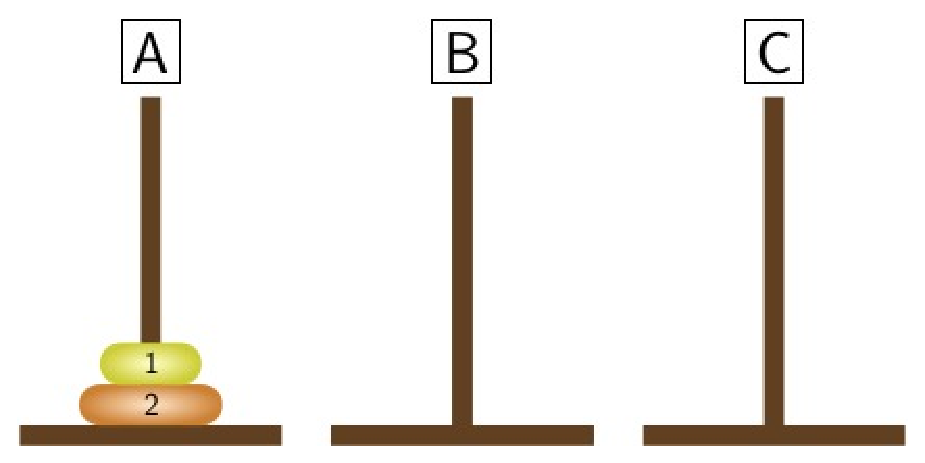
\includegraphics[width=50mm]{./H21}
&
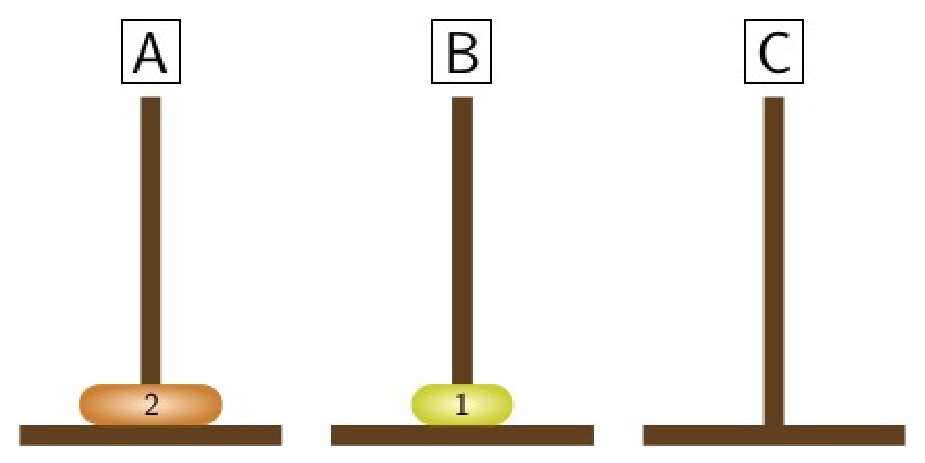
\includegraphics[width=50mm]{./H22}
\end{tabular}
\end{center}
Now we move the disk from peg $A$ to peg $C$.
\begin{center}
\begin{tabular}{l|r}
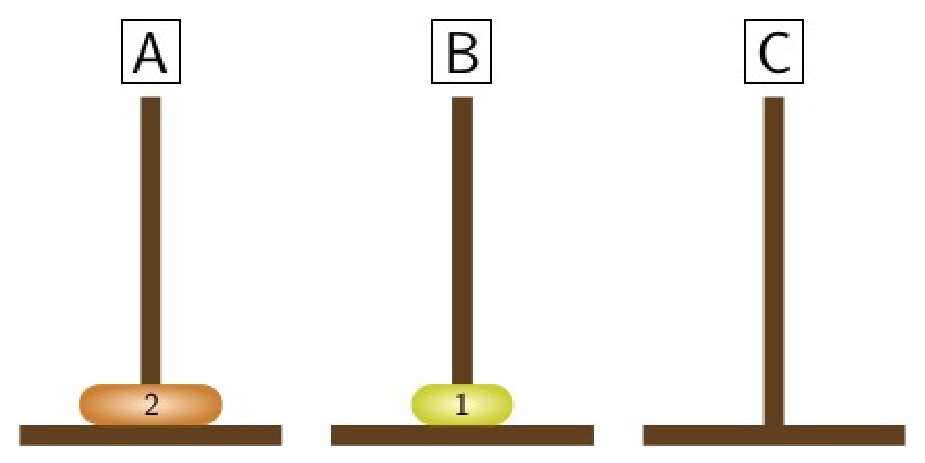
\includegraphics[width=50mm]{./H22}
&
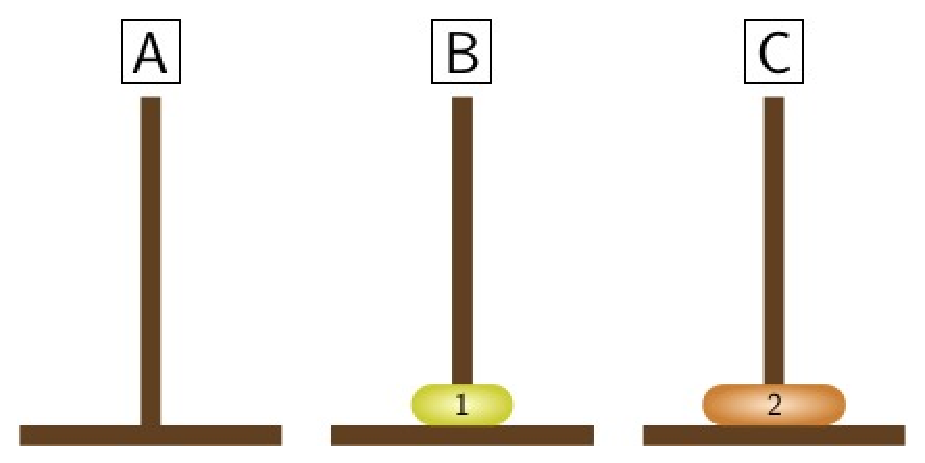
\includegraphics[width=50mm]{./H23}
\end{tabular}
\end{center}
Finally, we move the disk from peg $B$ to peg $C$.
\begin{center}
\begin{tabular}{l|r}
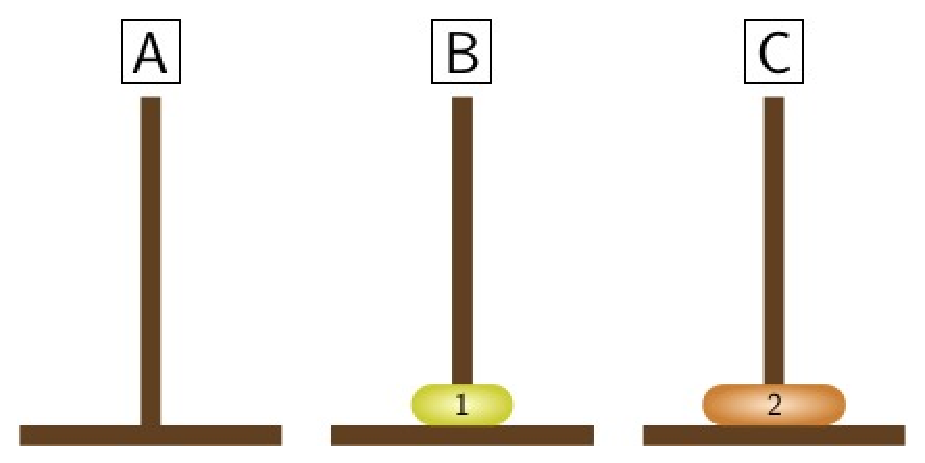
\includegraphics[width=50mm]{./H23}
&
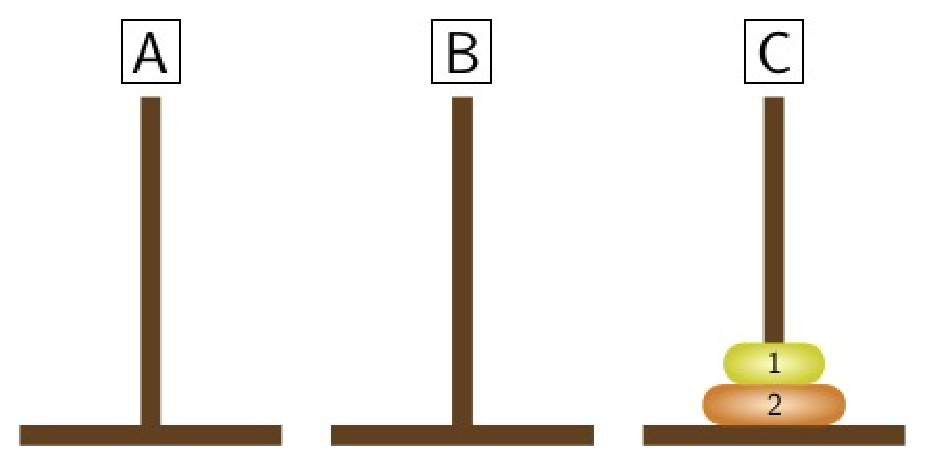
\includegraphics[width=50mm]{./H24}
\end{tabular}
\end{center}
Let us denote by $T_n$ the  minimum number of moves
that will transfer $n$ disks from peg $A$ to peg $C$.
Since no moves are needed to transfer $n=0$ disks, we have that $T_0=0$,
and the previous two examples show that $T_1=1$ and $T_2=3$.
Let us prove that $T_n\leq 2T_{n-1}+1$, that is, there is a solution with $2T_{n-1}+1$ moves.
In $T_{n-1}$ moves we can transfer the $n-1$ smaller disks from peg $A$ to peg $B$. We move the largest
one from peg $A$ to peg $C$ and it remains to move the $n-1$ smallest disks from peg $B$ to peg $C$ and
it can be done in $T_{n-1}$ moves. In total this strategy requires $2T_{n-1}+1$ moves. We only have to show
that $2T_{n-1}+1$ moves are necessary.
If we follow another strategy, then we must move the
largest disk at some point and the $n-1$ smallest disks must be on a single peg (requiring $T_{n-1}$ moves).
After moving the largest disk we must transfer the $n-1$ smallest disks to peg $C$ (requiring another $T_{n-1}$ moves).
It means that $T_n\geq 2T_{n-1}+1$, therefore
$$
T_n=2T_{n-1}+1.
$$
We apply the above strategy to present a minimal solution in case of 3 disks. First we move the 2 smallest disks from peg $A$
to peg $B$. It can be done in $T_2=3$ steps.

STEP 1:
\begin{center}
\begin{tabular}{l|r}
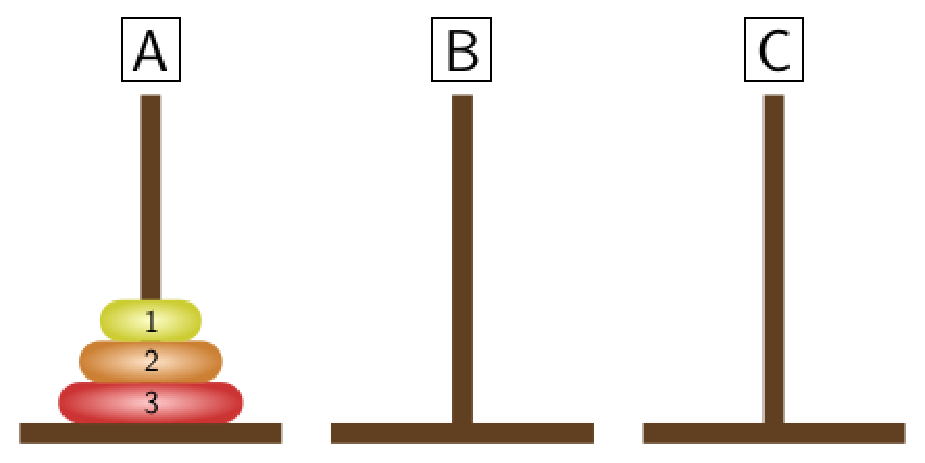
\includegraphics[width=50mm]{./H31-1}
&
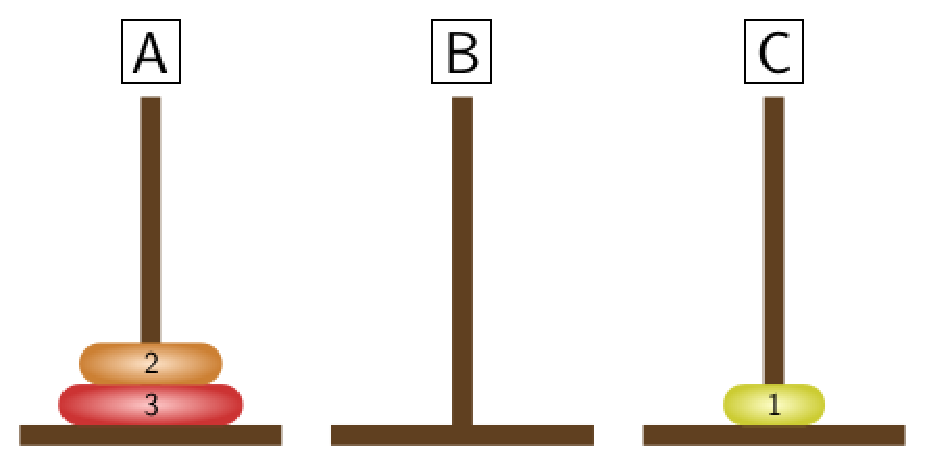
\includegraphics[width=50mm]{./H32-1}
\end{tabular}
\end{center}

STEP 2:
\begin{center}
\begin{tabular}{l|r}
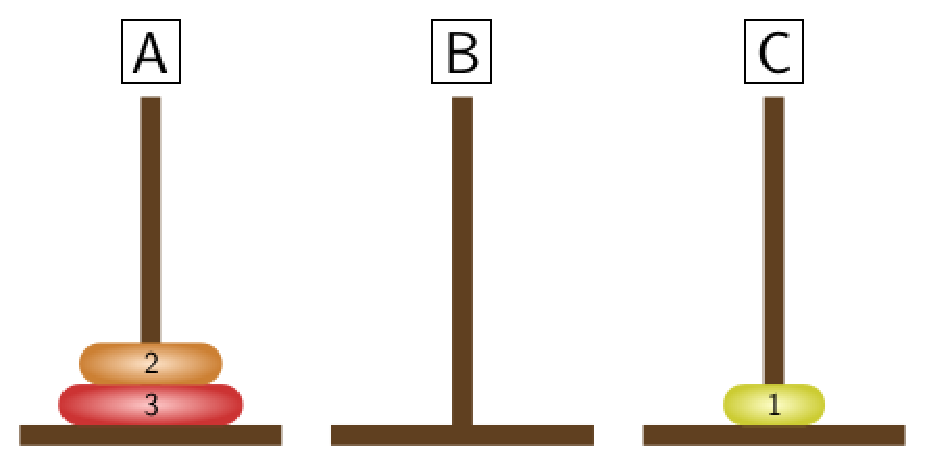
\includegraphics[width=50mm]{./H32-1}
&
\includegraphics[width=50mm]{./H33-1}
\end{tabular}
\end{center}

STEP 3:
\begin{center}
\begin{tabular}{l|r}
\includegraphics[width=50mm]{./H33-1}
&
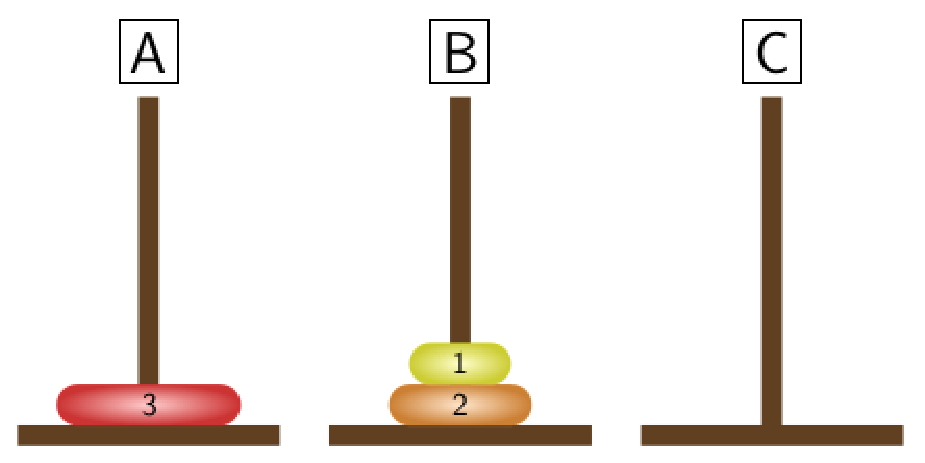
\includegraphics[width=50mm]{./H34-1}
\end{tabular}
\end{center}

Now we can transfer the largest disk to peg $C$.

STEP 4:
\begin{center}
\begin{tabular}{l|r}
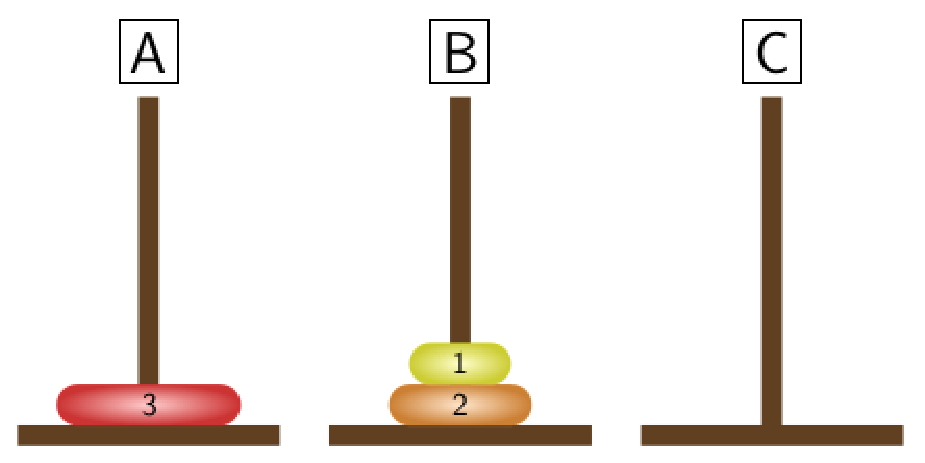
\includegraphics[width=50mm]{./H34-1}
&
\includegraphics[width=50mm]{./H35-1}
\end{tabular}
\end{center}

It remainst to transfer the 2 smallest disks from peg $B$ to peg $C$, it requires again $T_2=3$ moves.

STEP 5:
\begin{center}
\begin{tabular}{l|r}
\includegraphics[width=50mm]{./H35-1}
&
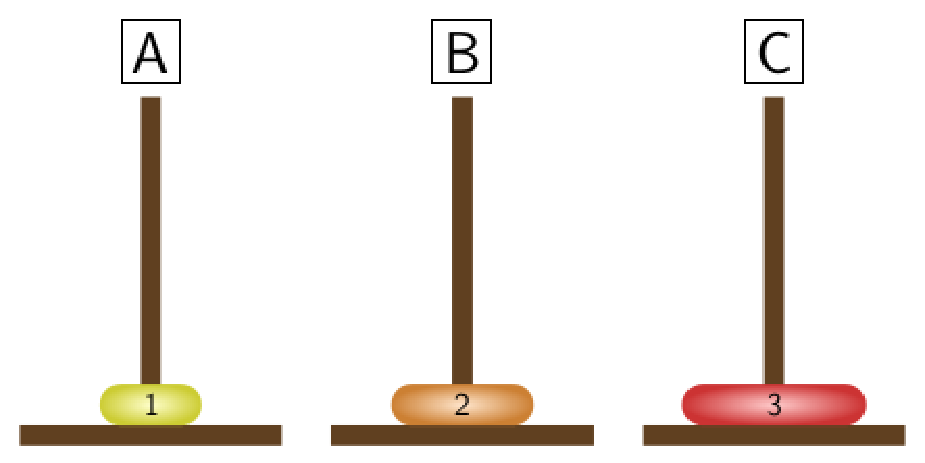
\includegraphics[width=50mm]{./H36-1}
\end{tabular}
\end{center}

STEP 6:
\begin{center}
\begin{tabular}{l|r}
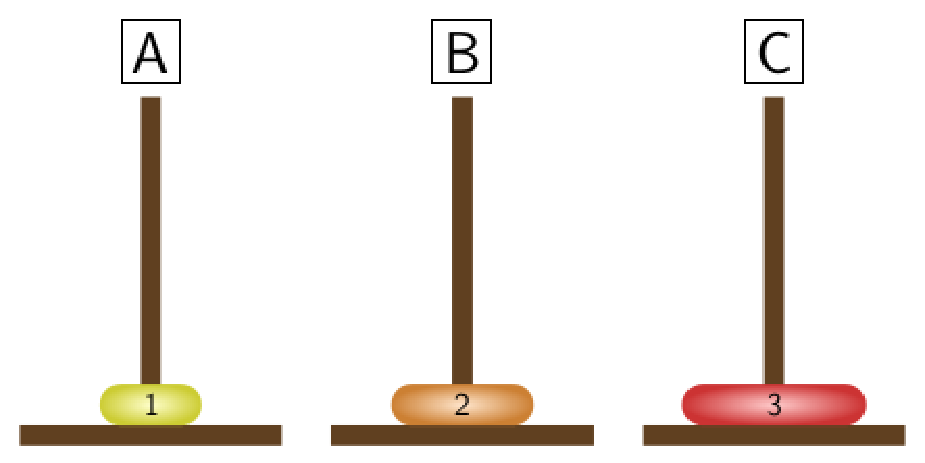
\includegraphics[width=50mm]{./H36-1}
&
\includegraphics[width=50mm]{./H37-1}
\end{tabular}
\end{center}

STEP 7:
\begin{center}
\begin{tabular}{l|r}
\includegraphics[width=50mm]{./H37-1}
&
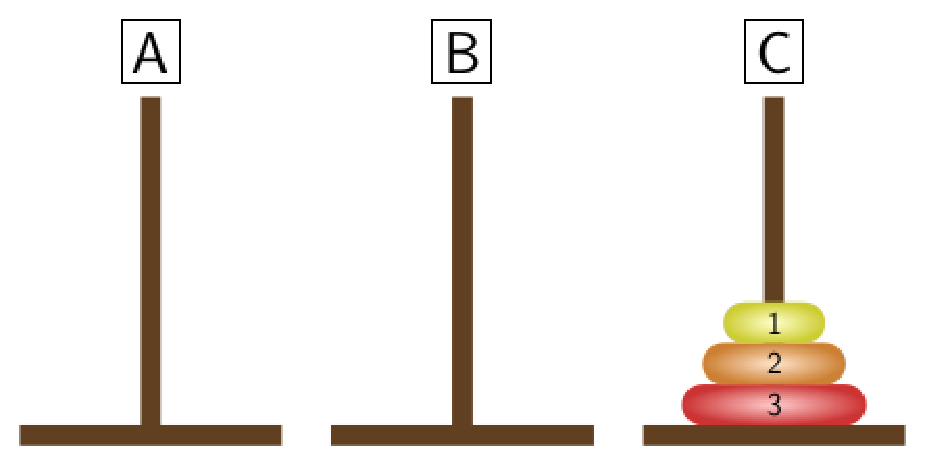
\includegraphics[width=50mm]{./H38-1}
\end{tabular}
\end{center}
Since $T_3=7$ we have found a solution with minimal number of moves.
Having a recurrence relation for the minimal number of moves may help to 
find a nice formula for $T_n$.
The following table contains the first few values of $T_n$.
\begin{center}
\begin{tabular}{|c|c||c|c||c|c|}
\hline
$n$ & $T_n$ & $n$ & $T_n$ & $n$ & $T_n$\\
\hline
0 & 0 & 4 & 15 & 8 & 255\\
\hline
1 & 1 & 5 & 31 & 9 & 511\\
\hline
2 & 3 & 6 & 63 & 10 & 1023\\
\hline
3 & 7 & 7 & 127 & 11 & 2047\\
\hline
\end{tabular}
\end{center}
One can easily observe that these values are 1 less than a power of 2, that is, 
we expect that $T_n=2^n-1$. It can be proved by induction.

\section{Linear recurrence relations of order $k$}
In this section by a sequence we mean an ordered list
$$
\halmaz{a_n}_{n=0}^{\infty},\quad a_n\in S
$$
for some set $S$.
For example 
$$
1,2,4,8,16,32,64,\ldots
$$
is a sequence containing non-negative powers of 2.
\begin{definition}
A sequence $\halmaz{a_n}_{n=0}^{\infty}$  is said to satisfy a \emph{linear recurrence} relation of order $k$ if
$$
a_n=c_{n-1}a_{n-1}+c_{n-2}a_{n-2}+\ldots+c_{n-k}a_{n-k}+b_n,\quad c_{n-k}\neq 0, n\geq k,
$$
where $c_{n-1},\ldots,c_{n-k},b_n$ are some constants. If $b_n=0$, then we say that the sequence
satisfies a \emph{homogeneous linear recurrence} relation of order $k$.
In case of a linear recurrence relation of order $k$ the values of $a_0,a_1,\ldots,a_{k-1}$
are called the \emph{initial values} of the sequence.
\end{definition}
For example the sequence appeared in case of Tower of Hanoi is a sequence of order 1:
\begin{align*}
T_0&=0,\\
T_n&=2T_{n-1}+1 \mbox{ for }n\geq 1.
\end{align*}
\begin{theorem}
Let $\halmaz{a_n}_{n=0}^{\infty}$ be a linear recurrence relation of order 1, that is, 
$$
a_n=ua_{n-1}+v
$$
for some constants $u,v$. If $u=1$, then 
$$
a_n=a_0+nv,
$$
otherwise
$$
a_n=u^na_0+\frac{u^n-1}{u-1}v.
$$
\end{theorem}
\begin{proof}
If $u=1$, then the defining equation simplifies as follows
$$
a_n=a_{n-1}+v.
$$
We prove the statement by induction.
The initial value of the sequence is $a_0$. Using the above formula for $a_n$ we obtain
\begin{align*}
a_1&=a_0+v,\\
a_2&=a_1+v=a_0+2v,\\
a_3&=a_2+v=a_0+3v.
\end{align*}
Hence the statement is clearly true for $n=1,2$ and 3. Assume that the statement is true
for $n=k$, that is, 
$$
a_k=a_0+kv.
$$
The statement for $n=k+1$ is that $a_{k+1}=a_0+(k+1)v$. By the recurrence definition we
have $a_{k+1}=a_{k}+v$. By induction we obtain that 
$$
a_{k+1}=a_0+kv+v=a_0+(k+1)v,
$$
which is the desired result for $n=k+1$.

Now assume that $u\neq 1$. We apply induction again. As in the previous case we compute the first few values of the sequence
\begin{align*}
a_1&=ua_0+v,\\
a_2&=ua_1+v=u^2a_0+uv+v,\\
a_3&=ua_2+v=u^3a_0+u^2v+uv+v.
\end{align*}
It follows that the statement is true if $n=1,2,3$. Assume that the statement is true
for $n=k$, that is, 
$$
a_k=u^ka_0+\frac{u^k-1}{u-1}v.
$$
We need to show that the statement is true for $n=k+1$, so $a_{k+1}=u^{k+1}a_0+\frac{u^{k+1}-1}{u-1}v$.
The recurrence definition yields that
$a_{k+1}=ua_{k}+v$. Using the assumption one has that
$$
a_{k+1}=ua_{k}+v=u\cdot \left(u^ka_0+\frac{u^k-1}{u-1}v\right)+v=u^{k+1}a_0+u\frac{u^k-1}{u-1}v+v.
$$
From the well-known identity $u^m-1=(u-1)\cdot (u^{m-1}+u^{m-2}+\ldots+u+1)$ one gets that 
$$
\frac{u^m-1}{u-1}=u^{m-1}+u^{m-2}+\ldots+u+1
$$
for $u\neq 1$. So we have $u\frac{u^k-1}{u-1}\cdot v+v=(u^k+u^{k-1}+\ldots+u)v+v=(u^k+u^{k-1}+\ldots+u+1)\cdot v$.
Finally we obtain that
$$
a_{k+1}=u^{k+1}a_0+(u^k+u^{k-1}+\ldots+u+1)v=u^{k+1}a_0+\frac{u^{k+1}-1}{u-1}v, 
$$
and the statement follows.
\end{proof}
It is easy to compute an explicit formula for the sequence $T_n$ related to the problem of Tower of Hanoi.
Here $T_n$ is defined as 
\begin{align*}
T_0&=0,\\
T_n&=2T_{n-1}+1 \mbox{ for }n\geq 1,
\end{align*}
that is, $u=2$ and $v=1$. The theorem implies that 
$$
T_n=u^nT_0+\frac{u^n-1}{u-1}v=2^n\cdot 0+\frac{2^n-1}{2-1}\cdot 1=2^n-1.
$$

Consider another example, let $a_n$ be a sequence defined by
\begin{align*}
a_0&=3,\\
a_n&=2a_{n-1}+2 \mbox{ for }n\geq 1.
\end{align*}
We apply the theorem and we have
$$
a_n=2^n\cdot 3+\frac{2^n-1}{2-1}\cdot 2=2^n\cdot 3+2^{n+1}-2=5\cdot 2^n-2.
$$

We have proved a theorem about linear recurrence relations of order 1, given such a recurrence
we are able to provide an explicit formula. What about higher order linear recurrence relations?
To make the presentation simpler we will consider homogeneous linear recurrence relations of order $k$,
where $k\geq 2$. So we study the structure of the recurrence given by
\begin{equation}\label{hlr}
a_n=c_{n-1}a_{n-1}+c_{n-2}a_{n-2}+\ldots+c_{n-k}a_{n-k},\quad c_{n-k}\neq 0, n\geq k,
\end{equation}
where $c_{n-1},\ldots,c_{n-k}$ are some constants.
\begin{theorem}\label{UV}
Assume that $U_n$ and $V_n$ are sequences satisfying \eqref{hlr} and $s,t$ are constants.
The linear combination
$$
W_n=sU_n+tV_n
$$
gives another solution of \eqref{hlr}.
\end{theorem}
\begin{proof}
Since $U_n$ and $V_n$ satisfy \eqref{hlr} we have
\begin{align*}
U_n&=c_{n-1}U_{n-1}+c_{n-2}U_{n-2}+\ldots+c_{n-k}U_{n-k},\\
V_n&=c_{n-1}V_{n-1}+c_{n-2}V_{n-2}+\ldots+c_{n-k}V_{n-k}.
\end{align*}
Substituting these formulas into the definition of $W_n$ we get
\begin{align*}
W_n=&s(c_{n-1}U_{n-1}+c_{n-2}U_{n-2}+\ldots+c_{n-k}U_{n-k})+\\
&t(c_{n-1}V_{n-1}+c_{n-2}V_{n-2}+\ldots+c_{n-k}V_{n-k})=\\
&c_{n-1}(sU_{n-1}+tV_{n-1})+c_{n-2}(sU_{n-2}+tV_{n-2})+\ldots+\\
&+c_{n-k}(sU_{n-k}+tV_{n-k})=\\
&c_{n-1}W_{n-1}+c_{n-2}W_{n-2}+\ldots+c_{n-k}W_{n-k}.
\end{align*}
It turned out that $W_n$ is also a solution of \eqref{hlr}.
\end{proof}
The previous theorem suggests a strategy to determine explicit formula
for higher order linear homogeneous recurrence relations. First we look for solutions
of the concrete recurrence relation, then we consider linear combinations of them
and we try to fix the constants in such a way that the initial values of the given sequence
are the same as in case of the sequence obtained by linear combination. What kind of solutions
should we look for? Here we need some numerical experiences. Consider the example
\begin{align*}
a_0&=2,\\
a_1&=2,\\
a_n&=2a_{n-1}+3a_{n-2},\quad n\geq 2.
\end{align*}
The above sequence is a homogeneous linear recurrence sequence of order $2$.
We can easily compute the first few elements of the sequence, $a_2=10, a_3=26, a_4=82$.
Let us consider the ratio of consecutive elements of the sequence.
\begin{center}
\begin{tabular}{|c|c||c|c|}
\hline
$n$ & $\frac{a_n}{a_{n-1}}$ & $n$ & $\frac{a_n}{a_{n-1}}$\\
\hline
1 & $1$ & 5 & $\approx 2.951$\\
\hline
2 & $5$ & 6 & $\approx 3.017$\\
\hline
3 & $2.6$ & 7 & $\approx 2.995$\\
\hline
4 & $\approx 3.154$ & 8 & $\approx 3.002$\\
\hline
\end{tabular}
\end{center}
The ratios are very close to a constant, in this case very close to 3 for $n\in\halmaz{4,5,6,7,8}$.
At the beginning of this chapter we studied sequences for which the ratio of consecutive elements
is a constant, these are geometric progressions. Let us look for geometric progressions satisfying
the same recurrence relation as $a_n$. If $g_n$ is a sequence given by
the formula
$$
g_n=rg_{n-1},
$$
where $r$ is the common ratio of the sequence with initial value $g_0$, then we have that 
$g_n=g_0r^n$. That is, $g_n$ is a geometric progression. Let us assume that for some initial
value $g_0$ and for some $r$ the progression satisfies the same recurrence relation as $a_n$.
Now we obtain
$$
g_n=2g_{n-1}+3g_{n-2}.
$$
It follows that
$$
g_0r^n=2g_0r^{n-1}+3g_0r^{n-2}.
$$
The constant zero progression is not useful for our purposes we assume that $g_0\neq 0$ and $r\neq 0$.
After dividing by $g_0r^{n-2}$ we get
$$
r^2=2r+3.
$$
If there is such a progression, then $r$ is a root of the quadratic polynomial $r^2-2r-3$.
One can determine the roots by the well-known formula, which is in our case
$$
\frac{2\pm\sqrt{4-4(-3)}}{2}.
$$
That is, the roots are $3$ and $-1$. We have two different solutions of the recurrence relation
and Theorem~\ref{UV} implies that linear combinations of these two solutions yield another solutions.
Let us consider the sequence $W_n=s3^n+t(-1)^n$. We should fix $s,t$ in such a way that 
\begin{align*}
&W_0=a_0=2,\\
&W_1=a_1=2.
\end{align*}
We get a system of equations in two unknowns
\begin{align*}
W_0=2&\Rightarrow s\cdot 3^0+t\cdot (-1)^0=2,\\
W_1=2&\Rightarrow s\cdot 3^1+t\cdot (-1)^1=2.
\end{align*}
The first equation implies that $t=2-s$. The second equation can be written as $3s+(2-s)(-1)=2$, that is, $4s=4$ and we get that $s=1,t=1$.
Now we have a sequence $W_n=3^n+(-1)^n$ which satisfies the appropriate recurrence relation and has the same initial values as $a_n$.
Thus $W_n=a_n$. In this way we obtained an explicit formula for the recurrence sequence $a_n$ given by
$$
3^n+(-1)^n.
$$
We may try to apply the above method to determine an explicit formula for the famous Fibonacci sequence:
\begin{align*}
F_0&=0,\\
F_1&=1,\\
F_n&=F_{n-1}+F_{n-2},\quad n\geq 2.
\end{align*}
Let $g_n$ be a geometric progression such that $g_n=g_0r^n$ for some $g_0$ and $r$.
Assume that $g_n$ satisfies the recurrence relation. It follows that
$$
r^2=r+1.
$$
The two roots of this quadratic polynomial are
$$
\frac{1-\sqrt{5}}{2}\quad\mbox{ and }\quad\frac{1+\sqrt{5}}{2}.
$$
Let $W_n$ be a linear combination of the appropriate geometric progressions, that is, 
$$
W_n=s\cdot \left(\frac{1-\sqrt{5}}{2}\right)^n+t\cdot \left(\frac{1+\sqrt{5}}{2}\right)^n.
$$
It remains to find $s$ and $t$ for which
\begin{align*}
&W_0=F_0=0,\\
&W_1=F_1=1.
\end{align*}
The above equations imply that
\begin{align*}
s+t&=0\\
s\cdot \left(\frac{1-\sqrt{5}}{2}\right)+t\cdot \left(\frac{1+\sqrt{5}}{2}\right)&=1.
\end{align*}
We immediately get that $t=-s$. Therefore
$$
s\cdot \left(\frac{1-\sqrt{5}}{2}\right)-s\cdot \left(\frac{1+\sqrt{5}}{2}\right)=1.
$$
The latter equation yields that $s=\frac{-\sqrt{5}}{5}$, so  $t=\frac{\sqrt{5}}{5}$.
The explicit formula in case of the Fibonacci sequence is
$$
F_n=\frac{-\sqrt{5}}{5}\cdot \left(\frac{1-\sqrt{5}}{2}\right)^n+\frac{\sqrt{5}}{5}\cdot \left(\frac{1+\sqrt{5}}{2}\right)^n.
$$
Let us see if the previous argument works for homogeneous linear recurrence sequence of order greater than 2.
We define $a_n$ as
\begin{align*}
a_0&=5,\\
a_1&=-3,\\
a_2&=11,\\
a_n&=-a_{n-1}+4a_{n-2}+4a_{n-3},\quad n\geq 3.
\end{align*}
The sequence $a_n$ is a homogeneous linear recurrence sequence of order 3, since $a_n$ depends on 
the previous 3 elements of the sequence. We try to find a geometric progression $g_n=g_0r^n$ satisfying
the above recurrence
$$
g_0r^n=-g_0r^{n-1}+4g_0r^{n-2}+4g_0r^{n-3}.
$$
Again we exclude the case $g_0r=0$, so we may simplify the equation by $g_0r^{n-3}$.
So we obtain
$$
r^3+r^2-4r-4=0.
$$
This time we have a cubic polynomial and finding the roots of a cubic is more difficult than determining
the roots of a quadratic polynomial. We may try to find some special roots e.g.\ integral roots. 
To find integral roots we can rewrite the equation in the form
$$
r\cdot (r^2+r-4)=4.
$$
If $r$ is an integer, then the expression on the left-hand side is a multiple of two integers. The multiple
of two integers is equal to 4, that is, we have only a few possibilities since $r$ has to divide 4. That
is $r\in\halmaz{-4,-2,-1,1,2,4}$. Evaluate the cubic polynomial at these values:
\begin{center}
\begin{tabular}{|c|c|}
\hline
$r$ & $r^3+r^2-4r-4$\\
\hline
-4 & -36\\
\hline
-2 & 0\\
\hline
-1 & 0\\
\hline
 1 & -6\\
 \hline
 2 & 0\\
 \hline
 4 & 60\\
 \hline
\end{tabular}
\end{center}
We are lucky, there are 3 integral roots: $-2,-1$ and 2. It means by Theorem~\ref{UV} that any linear combinations
of the geometric progressions $(-2)^n, (-1)^n$ and $2^n$ will satisfy the same recurrence relation as $a_n$.
Now define $W_n=s(-2)^n+t(-1)^n+u2^n$. Our task is to fix $s,t$ and $u$ such that
\begin{align*}
&W_0=a_0=5,\\
&W_1=a_1=-3,\\
&W_2=a_2=11.
\end{align*}
These equations yield a system of equations in three unknowns.
\begin{align*}
s+t+u&=5\\
-2s-t+2u&=-3\\
4s+t+4u&=11.
\end{align*}
We can eliminate $s$ and $u$ using the first and the third equations. To do so we multiply the first equation by 4:
\begin{align*}
4s+4t+4u&=20\\
-2s-t+2u&=-3\\
4s+t+4u&=11.
\end{align*}
We subtract the third equation from the first one and we get
$$
3t=9,
$$
that is, $t=3$. The system of equations can be simplified now:
\begin{align*}
s+u&=2\\
-2s+2u&=0.
\end{align*}
The second equation implies that $s=u$, so from the first equation we have that $s=u=1$.
The explicit formula for the sequence $a_n$ is
$$
(-2)^n+3\cdot (-1)^n+2^n.
$$

We remark that the previous argument does not work if we have a root with multiplicity greater than 1.
Without providing the details of the theory we note that it is also possible to handle such cases. For example
assume that a linear recurrence of order 2 is given and the corresponding quadratic polynomial has a double root $r$.
We have that $r^n$ and $nr^n$ are solutions of the same recurrence. In general, if we have a linear recurrence of order $k$
and the corresponding polynomial has a root $r$ with multiplicity $m$, then 
$$
r^n,\quad nr^n,\ldots n^{m-1}r^n
$$
are solutions of the same recurrence.
Let us consider an example.
\begin{align*}
u_0&=4,\\
u_1&=-1,\\
u_2&=-1,\\
u_3&=-43,\\
u_n&=5u_{n-1}-6u_{n-2}-4u_{n-3}+8u_{n-4},\quad n\geq 4.
\end{align*}
The corresponding quartic polynomial $r^4-5r^3+6r^2+4r-8$ can be written as $(r+1)(r-2)^3$,
that is, $-1$ is a simple root and 2 is a root with multiplicity 3. Therefore we define $W_n$ as
$$
s\cdot (-1)^n+t\cdot 2^n+xn\cdot 2^n+yn^2\cdot 2^n.
$$
Then we obtain four equations in four unknowns
\begin{align*}
s+t&=4\\
-s+2t+2x+2y&=-1\\
s+4t+8x+16y&=-1\\
-s+8t+24x+72y&=-43.
\end{align*}
We get that $s=4-t$, hence
\begin{align*}
3t+2x+2y&=3\\
3t+8x+16y&=-5\\
9t+24x+72y&=-39.
\end{align*}
Using the first equation we can eliminate $t$ from the second and the third equations.
\begin{align*}
6x+14y&=-8\\
18x+66y&=-48.
\end{align*}
The above system has the solution $x=1, y=-1$. We get that $t=1$ and $s=3$.
Thus
$$
u_n=3\cdot (-1)^n+2^n+n\cdot 2^n-n^2\cdot 2^n.
$$
As an application we deal with an inverse problem, let us be given the sequence
$$
u_n=\left(\frac{3-\sqrt{33}}{2}\right)^n+\left(\frac{3+\sqrt{33}}{2}\right)^n,\quad n\geq 0.
$$
Our statement is that $u_n$ is an integer sequence and 3 divides $u_n$ for $n\geq 1$. This statement
can be proved by induction (Exercise~\ref{induction-6}), but now we apply the theory of linear recurrence sequences. We are given an
explicit formula and we would like to determine a linear recurrence sequence which has the same closed-form
solution. It is easy to see that $u_0=2$ and $u_1=3$. If we have an appropriate recurrence, then $\frac{3-\sqrt{33}}{2}$
and $\frac{3+\sqrt{33}}{2}$ are roots of some quadratic polynomial:
$$
\left(r-\frac{3-\sqrt{33}}{2}\right)\cdot \left(r-\frac{3+\sqrt{33}}{2}\right)=r^2-3r-6.
$$
From this polynomial we have the following recurrence relation $u_n=3u_{n-1}+6u_{n-2}$.
That is, we have a recurrence sequence
\begin{align*}
u_0&=2,\\
u_1&=3,\\
u_n&=3u_{n-1}+6u_{n-2}=3(u_{n-1}+2u_{n-2}).
\end{align*}
Since $u_0$ and $u_1$ are integers and $u_{n-1},u_{n-2}$ have integral coefficients in the recurrence relation, the sequence $u_n$
is an integral sequence. It is clear that $u_1=3$ is divisible by 3 and similarly $u_n=3(u_{n-1}+2u_{n-2})$ is a multiple of 3.

\begin{exercise}\label{seq-ex-1}
Find the shortest sequence of moves that transfers a tower of 4
disks from peg $A$ to peg $C$.
\end{exercise}

\begin{exercise}\label{seq-ex-2}
Find a closed-form formula for the following sequence defined by:
$$
a_n=7a_{n-1}-10a_{n-2}\quad\mbox{ for }n\geq 2\quad\mbox{ and }a_0=0,a_1=2.
$$
\end{exercise}

\begin{exercise}\label{seq-ex-3}
Find an explicit formula for the following sequence defined by:
$$
a_n=4a_{n-1}-3a_{n-2}\quad\mbox{ for }n\geq 2\quad\mbox{ and }a_0=1,a_1=13.
$$
\end{exercise}

\begin{exercise}\label{seq-ex-4}
Find a closed-form formula for the following sequence defined by:
$$
a_n=-2a_{n-1}+a_{n-2}+2a_{n-3}\quad\mbox{ for }n\geq 3\quad\mbox{ and }a_0=0,a_1=1,a_2=2.
$$
\end{exercise}

\begin{exercise}\label{seq-ex-5}
Find an explicit formula for the following sequence defined by:
$$
a_n=6a_{n-1}-11a_{n-2}+6a_{n-3}\quad\mbox{ for }n\geq 3\quad\mbox{ and }a_0=0,a_1=0,a_2=1.
$$
\end{exercise}

\begin{exercise}\label{seq-ex-6}
Find a closed-form formula for the following sequence defined by:
$$
a_n=4a_{n-1}-4a_{n-2}\quad\mbox{ for }n\geq 2\quad\mbox{ and }a_0=-1,a_1=0.
$$
\end{exercise}

\begin{exercise}\label{seq-ex-7}
Find an explicit formula for the following sequence defined by:
$$
a_n=5a_{n-1}-3a_{n-2}-9a_{n-3}\quad\mbox{ for }n\geq 3\quad\mbox{ and }a_0=3,a_1=4,a_2=29.
$$
\end{exercise}

\begin{exercise}\label{seq-ex-8}
Prove that the sequence defined by
$$
u_n=\left(\frac{5-3\sqrt{5}}{2}\right)^n+\left(\frac{5+3\sqrt{5}}{2}\right)^n,\quad n\geq 0
$$
contains only integers and $u_n$ is divisible by 5 if $n\geq 1$.
\end{exercise}

\begin{exercise}\label{seq-ex-9}
Prove that the sequence defined by
$$
(4-\sqrt{2})^n+(4+\sqrt{2})^n,\quad n\geq 0
$$
contains only integers divisible by 2.
\end{exercise}


% !TEX root = lectnote.tex
% !TEX spellcheck = en_GB-oed 

\chapter{Solutions}\label{cha:solutions}

\section{Introduction}
\begin{enumerate}
\item[\ref{intro-ex-1}]
There are three given sets $A=\halmaz{3,4,6,7,8},B=\halmaz{2,4,5,6,8}$ and $C=\halmaz{1,2,4,5,8}$. 
We have that
\begin{align*}
A\setminus B&=\halmaz{3,7}\\
C\cap B&=\halmaz{2,4,5,8}.
\end{align*}
Thus 
$$
(A\setminus B)\cup(C\cap B)=\halmaz{2,3,4,5,7,8}.
$$

\item[\ref{intro-ex-2}]
We have three sets $A=\halmaz{1,3,4,6,7},B=\halmaz{2,4,5,6,8}$ and $C=\halmaz{1,3,4,5,8}$. 
\begin{align*}
(A\cap B)&=\halmaz{4,6}\\
(C\cap B)&=\halmaz{4,5,8}.
\end{align*}
Therefore
$$
(A\cap B)\setminus(C\cap B)=\halmaz{6}.
$$

\item[\ref{intro-ex-3}]
Now the three given sets are $A=\halmaz{1,3,4,6,7},B=\halmaz{2,4,6,8}$ and $C=\halmaz{1,3,4,8}$. 
\begin{align*}
(A\setminus B)&=\halmaz{1,3,7}\\
(C\setminus B)&=\halmaz{1,3}.
\end{align*}
So we obtain
$$
(A\setminus B)\cup(C\setminus B)=\halmaz{1,3,7}.
$$

\item[\ref{intro-ex-4}]

(a) The elements of the set are 7, 10 and 13.

(b) The elements of the set are 0, 1 and 4.

(c) The possible differences are $3-1, 3-2, 4-1, 4-2, 5-1$ and $5-2$, thus the elements of the set are 1, 2, 3 and 4.

\item[\ref{intro-ex-5}]

(a) $\halmazvonal{2k}{ k\in\halmaz{1,2,3,4,5}}$, 

(b) $\halmazvonal{k^2}{k\in\halmaz{1,2,3,4,5}}$, 

(c) $\halmazvonal{2^{-k}}{ k\in\mathbb{N}\cup\halmaz{0}}$,

(d) $\halmazvonal{a/b }{a,b\in\mathbb{N}, b\leq a\leq 2b}$. 

\item[\ref{intro-ex-6}]

(a) 
\begin{center}
\begin{venndiagram3sets}
\fillACapB\fillC
\end{venndiagram3sets}
\end{center}

(b)
\begin{center}
\begin{venndiagram3sets}
\fillANotB\fillANotC
\end{venndiagram3sets}
\end{center}

(c)
\begin{center}
\begin{venndiagram3sets}
\fillACapC\fillBCapC
\end{venndiagram3sets}
\end{center}

(d)
\begin{center}
\begin{venndiagram3sets}
\fillACapC\fillBCapC\fillACapB
\end{venndiagram3sets}
\end{center}

(e)
\begin{center}
\begin{venndiagram3sets}
\fillACapBNotC\fillBCapCNotA\fillACapCNotB
\end{venndiagram3sets}
\end{center}

(f)
\begin{center}
\begin{venndiagram3sets}
\fillANotB\fillBNotC\fillCNotA
\end{venndiagram3sets}
\end{center}

\item[\ref{intro-ex-7}]
The set $A\cap B\cap C$ is a subset of all other sets for which we have certain cardinality conditions, so we may set
$$
A\cap B\cap C=\halmaz{1,2}.
$$
The conditions for $|A\cap B|, |A\cap C|$ and $|B\cap C|$ are satisfied. We have that $|A|=4$, that means that two elements
are missing from $A\setminus(B\cup C)$. We let $A\setminus(B\cup C)=\halmaz{3,4}$. Similarly for $B\setminus(A\cup C)$ and $C\setminus(A\cup B)$. We obtain that
\begin{center}
\begin{venndiagram3sets}[labelABC={\tiny{1,2}},labelOnlyA={\tiny{3,4}},labelOnlyB={\tiny{5,6}},labelOnlyC={\tiny{7,8}}]
\end{venndiagram3sets}
\end{center}

\item[\ref{intro-ex-8}]
Following the solution of Exercise \ref{intro-ex-7} we get:
\begin{center}
\begin{venndiagram3sets}[labelABC={\tiny{1,2}},labelOnlyBC={\tiny{3}},labelOnlyA={\tiny{4,5}},labelOnlyB={\tiny{6,7}},labelOnlyC={\tiny{8,9,10}}]
\end{venndiagram3sets}
\end{center}

\item[\ref{intro-ex-9}]

(a) $\sum_{i=4}^7 i=4+5+6+7$,

(b) $\sum_{i=1}^5 (i^2-i)=0+2+6+12+20$,

(c) $\sum_{i=1}^4 10^i=10+100+1000+10000$,

(d) $\sum_{2\leq i\leq 5} \frac{1}{2^i}=\frac{1}{4}+\frac{1}{8}+\frac{1}{16}+\frac{1}{32}$,

(e) $\sum_{i\in S} (-1)^i$, where $S=\halmaz{2,3,5,8}$ is $1+(-1)+(-1)+1$.



\item[\ref{intro-ex-10}]

(a) $2+4+6+8+10=\sum_{i=1}^5 2i$,

(b) $1+4+7+10=\sum_{i=0}^3 (3i+1)$,

(c) $\frac{1}{4}+\frac{1}{2}+1+2+4=\sum_{i=-2}^2 2^i$,

(d) $\frac{1}{4}-\frac{1}{2}+1-2+4=\sum_{i=-2}^2 (-2)^i$.

\item[\ref{intro-ex-11}]

(a) $\prod_{i=-4}^{-1} i=(-4)\cdot(-3)\cdot(-2)\cdot(-1)$,

(b) $\prod_{i=1}^4 (i^2)=1\cdot 4\cdot 9\cdot 16$,

(c) $\prod_{i=1}^3 2^i=2\cdot 4\cdot 8$,

(d) $\prod_{-2\leq i\leq 3} \frac{1}{2^i}=4\cdot 2\cdot 1\cdot \frac{1}{2}\cdot \frac{1}{4}\cdot \frac{1}{8}$,

(e) $\prod_{i\in S} (-1)^i$, where $S=\halmaz{2,4,6,7}$ is $(-1)^2\cdot(-1)^4\cdot(-1)^6\cdot(-1)^7$.

\item[\ref{intro-ex-12}]

(a) $1\cdot 3\cdot 5\cdot 7=\prod_{i=0}^3 (2i+1)$,

(b) $(-1)\cdot 2\cdot 5\cdot 8=\prod_{i=0}^3 (3i-1)$,

(c) $\frac{1}{9}\cdot\frac{1}{3}\cdot 1\cdot 3\cdot 9=\prod_{i=-2}^2 3^{i}$.




\item[\ref{ex:factorial1}]
The values are
\begin{align*}
0! &= 1, \\
1! &= 1, \\
2! &= 2, \\
3! &= 6, \\
4! &= 24, \\
5! &= 120, \\
6! &= 720, \\
7! &= 5~040, \\
8! &= 40~320.
\end{align*}

\item[\ref{ex:factorial2}]
The values are
\begin{align*}
5+3! &= 5+6 = 11, \\
(5+3)! = 8! &= 40~320, \\
4-2\cdot 3! &= 4-2\cdot 6 = 4-12=-8, \\
(4-2)\cdot 3! &= (4-2) \cdot 6 = 2 \cdot 6 = 12, \\
4 - (2 \cdot 3)! &= 4 - 6! = 4 - 720 = -716, \\
3 \cdot 2! &= 3 \cdot 2 = 6, \\
(3 \cdot 2)! &= 6! = 720, \\
4 \cdot 3! &= 4 \cdot 6 = 24, \\
4! \cdot 5 &= 24 \cdot 5 = 120. 
\end{align*}

\item[\ref{ex:factorial3}]
Let 
\[
S_n = \halmazvonal{k}{k \text{ is a positive integer}, k\leq n} = \halmaz{1, 2, \dots , n}. 
\]
Then it is easy to see that $S_n = S_{n-1} \cup \halmaz{n}$, 
that is, $S_n$ is the disjoint union of $S_{n-1}$ and $\halmaz{n}$. 
Then by the definition of the factorial, 
we have 
\[
n! = \prod_{k \in S_n} k = \left( \prod_{k \in \halmaz{n}} k \right) \cdot \left( \prod_{k \in S_{n-1}} k \right) = n \cdot (n-1)!. 
\]
If $n \geq 2$, then another proof could be 
\[
n! = n \cdot \underbrace{(n-1) \cdot (n-2) \cdot \dots \cdot 2 \cdot 1 }_{(n-1)!}= n \cdot (n-1)!. 
\]
Nevertheless, the claim is true for $n=1$, as well: 
\[
1! = 1 = 1 \cdot 1 = 1 \cdot 0!. 
\]


\item[\ref{intro-ex-13}]

(a) We obtain that
\begin{align*}
678 &= 1\cdot 567+111\\
567 &= 5\cdot 111+12\\
111 &= 9\cdot 12+3\\
12 &= 4\cdot 3+0.
\end{align*}
Thus $\gcd(678,567)=3$. We work backwards to compute $x$ and $y:$
\begin{align*}
3&=111-9\cdot 12\\
 &=111-9\cdot (567-5\cdot 111)=-9\cdot 567+46\cdot 111\\
 &=-9\cdot 567+46 \cdot (678-567)=46\cdot 678-55\cdot 567.
\end{align*}
Hence we have
$$
46\cdot 678-55\cdot 567=\gcd(678,567)=3.
$$

(b) We get that
\begin{align*}
803 &= 2\cdot 319+165\\
 319 &= 1\cdot 165+154\\
 165 &= 1\cdot 154+11\\
 154 &= 14\cdot 11+0.
\end{align*}
It follows that $\gcd(803,319)=11$. Now we find $x$ and $y:$
\begin{align*}
11&= 165-154\\
  &= 165-(319-165)=-319+2\cdot 165\\
  &= -319+2 \cdot (803-2\cdot 319)=2\cdot 803-5\cdot 319.
\end{align*}
So we get the equation
$$
2\cdot 803-5\cdot 319=\gcd(803,319)=11.
$$

(c) In this case the computations go as follows
\begin{align*}
2701 &= 1\cdot 2257+444\\
 2257 &= 5\cdot 444+37\\
 444 &= 12\cdot 37+0.
\end{align*}
Therefore $\gcd(2701,2257)=37$. We determine $x$ and $y:$
\begin{align*}
37&= 2257-5\cdot 444\\
  &= 2257-5(2701-2257)=-5\cdot 2701+6\cdot 2257.
\end{align*}
We have that 
$$
-5\cdot 2701+6\cdot 2257=\gcd(2701,2257)=37.
$$

(d) The summary of the computations:
\begin{align*}
3397 &= 1\cdot 1849+1548\\
 1849 &= 1\cdot 1548+301\\
 1548 &= 5\cdot 301+43\\
 301 &= 7\cdot 43+0.
\end{align*}
That is, $\gcd(3397,1849)=43$. It remains to compute $x$ and $y:$
\begin{align*}
43&=1548-5\cdot 301\\
  &=1548-5(1849-1548)=-5\cdot 1849+6\cdot 1548\\
  &= -5\cdot 1849+6(3397-1849)=6\cdot 3397-11\cdot 1849.
\end{align*}
Thus we obtain the equation
$$
6\cdot 3397-11\cdot 1849=\gcd(3397,1849)=43.
$$



\item[\ref{ex:numsyst1}]

Write 21 in base 2 first. 
Now, 16 is the highest 2-power not greater than 21, 
$21 = 1 \cdot 16 +5$, 
and we continue with the remainder 5. 
Now, 4 is the highest 2-power not greater than 5, 
$5 = 1\cdot 4 + 1$, 
and we continue with the remainder 1. 
Finally, 1 is the highest 2-power not greater than 1, 
$1 = 1 \cdot 1 + 0$. 
Thus 
\[
21_{10} = 1 \cdot 16 + 1 \cdot 4 + 1\cdot 1 = 1 \cdot 2^4 + 1 \cdot 2^2 + 1 \cdot 2^0 = 10101_2. 
\]

Now, write 50 in base 3. 
Here, 27 is the highest 3-power not greater than 50, 
$50 = 1 \cdot 27 + 23$, 
and we continue with the remainder 23. 
Now, 9 is the highest 3-power not greater than 23, 
$23 = 2\cdot 9 + 5$, 
and we continue with the remainder 5. 
Now, 3 is the highest 3-power not greater than 5, 
$5 = 1\cdot 3 + 2$, 
and we continue with the remainder 2. 
Finally, 1 is the highest 3-power not greater than 2, 
$2 = 2 \cdot 1 + 0$. 
Thus 
\[
50_{10} = 1 \cdot 27 + 2 \cdot 9 + 1 \cdot 3 + 2\cdot 1 = 1 \cdot 3^3 + 2 \cdot 3^2 + 1 \cdot 3^1 + 2 \cdot 3^0  = 1212_3. 
\]

Finally, write 2814 in base 16. 
Now, 256 is the highest 16-power not greater than 2814 
(the next 16-power is 4096), 
$2814 = 10 \cdot 256 + 254$, 
and we continue with the remainder 254. 
Now, 16 is the highest 16-power not greater than 254, 
$254 = 15\cdot 16 + 14$, 
and we continue with the remainder 14. 
Finally, 1 is the highest 16-power not greater than 14, 
$14 = 14 \cdot 1 + 0$. 
Thus 
\[
2814_{10} = 10 \cdot 256 + 15 \cdot 16 + 14 \cdot 1 = 10 \cdot 16^2 + 15 \cdot 16^1 + 14 \cdot 16^0   = AFE_{16}. 
\]


\item[\ref{ex:numsyst2}]

Rewrite $21_{10}$ into base 2 first. 
\begin{align*}
21 &= 10 \cdot 2 + 1, \\
10 &= 5 \cdot 2 + 0, \\
5 &= 2 \cdot 2 + 1, \\
2 &= 1 \cdot 2 + 0, \\
1 &= 0 \cdot 2 + 1. 
\end{align*}
The remainders backwards are 1, 0, 1, 0, 1, thus 
\[
21_{10} = 10101_{2}. 
\]

Now, rewrite $50_{10}$ into base 3. 
\begin{align*}
50 &= 16 \cdot 3 + 2, \\
16 &= 5 \cdot 3 + 1, \\
5 &= 1 \cdot 3 + 2, \\
1 &= 0 \cdot 3 + 1. 
\end{align*}
The remainders backwards are 1, 2, 1, 2, thus 
\[
50_{10} = 1212_{3}. 
\]

Finally, rewrite $250_{10}$ into base 8. 
\begin{align*}
250 &= 31 \cdot 8 + 2, \\
31 &= 3 \cdot 8 + 7, \\
3 &= 0 \cdot 8 + 3. 
\end{align*}
The remainders backwards are 3, 7, 2, thus 
\[
250_{10} = 372_{8}. 
\]

\item[\ref{ex:numsyst3}]
\begin{enumerate}
\item
\begin{align*}
111001101_2 &= 461_{10}, \\
1010101_2 &= 85_{10}, \\
11111_2 &= 31_{10}, \\
10110_2 &= 22_{10}, \\
101010101_2 &= 341_{10}, \\
10001000_2 &= 136_{10}, \\
1010111_2 &= 87_{10}, \\
111101_2 &= 61_{10}, \\
21102_3 &= 200_{10}, \\
1234_5 &= 194_{10}, \\
1234_7 &= 466_{10}, \\
1234_8 &= 668_{10}, \\
777_8 &= 511_{10}, \\
345_8 &= 229_{10}, \\ 
2012_8 &= 1034_{10}, \\
4565_8 &= 2421_{10}, \\
1123_8 &= 595_{10}, \\
666_8 &= 438_{10}, \\
741_8 &= 481_{10}, \\
CAB_{16} &= 3243_{10}, \\ 
BEE_{16} &= 3054_{10}, \\
EEE_{16} &= 3822_{10}, \\
4D4_{16} &= 1236_{10}, \\
ABC_{16} &= 2748_{10}, \\
9B5_{16} &= 2485_{10}, \\
DDD_{16} &=3549_{10}, \\
3F2_{16} &= 1010_{10}.
\end{align*}

\item
\begin{align*}
64_{10} &= 100 0000_2 = 2101_3 = 224_5 = 121_7 = 100_8 = 71_9 = 40_{16}, \\
50_{10} &= 11 0010_2 = 1212_3 = 200_5 = 101_7 = 62_8 = 55_9 = 32_{16}, \\
16_{10} &= 1 0000_2 = 121_3 = 31_5 = 22_7 = 20_8 = 17_9 = 10_{16}, \\
100_{10} &= 110 0100_2 = 1 0201_3 = 400_5 = 202_7 = 144_8 = 121_9 \\
&= 64_{16}, \\
2012_{10} &= 111 1101 1100_2 = 220 2112_3 = 3 1022_5 = 5603_7 = 3734_8 \\
&= 2675_9 = 7DC_{16}, \\
200_{10} &= 1100 1000_2 = 2 1102_3 = 1300_5 = 404_7 = 310_8 = 242_9 \\
&= C8_{16}, \\
151_{10} &= 1001 0111_2 = 1 2121_3 = 1101_5 = 304_7 = 227_8 = 177_9 \\
&= 97_{16}, \\
48_{10} &= 11 0000_2 = 1210_3 = 143_5 = 66_7 = 60_8 = 53_9 = 30_{16}, \\
99_{10} &= 110 0011_2 = 1 0200_3 = 344_5 = 201_7 = 143_8 = 120_9 \\
&= 63_{16}, \\
999_{10} &= 11 1110 0111_2 = 110 1000_3 = 1 2444_5 = 2625_7 = 1747_8 \\
&= 1330_9 = 3E7_{16}. 
\end{align*}

\item
\begin{align*}
1121_3 &= 43_{10} = 101011_2, \\
4312_5 &= 582_{10} = 1461_7, \\
654_8 &= 428_{10} = 525_9, \\
AD2_{16} &= 2770_{10} = 11035_7, \\
543_8 &= 355_{10} = 111011_3, \\
543_9 &= 444_{10} = 121110_3. 
\end{align*}

\item
\begin{align*}
777_8 &= 111111111_2 = 1FF_{16}, \\
345_8 &= 11100101_2 = E5_{16}, \\
2012_8 &= 10000001010_2 = 40A_{16}, \\
456_8 &= 100101110_2 = 12E_{16}, \\
235_8 &= 10011101_2 = 9D_{16}, \\
147_8 &= 1100111_2 = 67_{16}, \\
741_8 &= 111100001_2 = 1E1_{16}, \\ 
CAB_{16} &= 110010101011_2 = 6253_8, \\
BEE_{16} &= 101111101110_2 = 5756_8, \\
EEE_{16} &= 111011101110_2 = 7356_8, \\
4D3_{16} &= 10011010011_2 = 2323_8, \\
ABC_{16} &= 101010111100_2 = 5274_8, \\
FEE_{16} &= 111111101110_2 = 7756_8, \\
9B5_{16} &= 100110110101_2 = 4665_8, \\
3F2_{16} &= 1111110010_2 = 1762_8. 
\end{align*}

\end{enumerate}


\end{enumerate}
\newpage
\section{Counting}

\begin{enumerate}

\item[\ref{ex:sumk}]
Let $n$ be odd first, 
like it was with $n=199$. 
Then if we rearrange the summands (first with last, second with one but last, etc.). 
then the middle term will remain, 
which is $\frac{n+1}{2}$: 
\begin{align*}
& 1 + 2 + \dots + \left(n-1\right) + n = \left(1 + n\right) + \left(2 + n-1\right) + \dots \\
&+ \left(\frac{n-1}{2} + \frac{n+3}{2} \right) + \frac{n+1}{2} = (n+1) + (n+1) + \dots \\
&+ (n+1) +  \frac{n+1}{2} = \left( n+1 \right) \cdot \frac{n-1}{2} + \frac{n+1}{2} \\
&= \left( n+1 \right) \cdot \left( \frac{n-1}{2} + \frac{1}{2} \right) = \frac{(n+1) \cdot n}{2}. 
\end{align*}
If $n$ is even, 
then after rearranging the summands, no term will remain: 
\begin{align*}
& 1 + 2 + \dots + \left(n-1\right) + n = \left(1 + n\right) + \left(2 + n-1\right) + \dots \\
&+ \left(\frac{n}{2} + \frac{n+2}{2} \right) = (n+1) + (n+1) + \dots \\
&+ (n+1) = \left( n+1 \right) \cdot \frac{n}{2} = \frac{(n+1) \cdot n}{2}. 
\end{align*}

\item[\ref{ex:5people3hanshake}]
If everyone shakes hands with three other, 
then they do not shake hand with exactly one person. 
It is easier to consider who does not shake hand with whom. 
The first person does not shake hand with someone. 
Then of the remaining three people the first does not shake hand with someone from these three. 
That leaves one person, who does not shake hand with someone else, 
but everybody else has already been accounted for about not shaking hands with somebody. 
Thus, it is not possible that each of the five people shake hands with three others. 

This argument does not work if someone is allowed to shake hands with someone else more than once. 
Nevertheless, the answer is still \emph{no}. 
Use the same argument we used for proving Corollary~\ref{cor:handshakes}. 
If we sum up all the handshakes for everyone, we obtain $5 \cdot 3 = 15$, 
as each of the 5 people shakes hand with 3 others. 
This way, we counted every handshake twice, 
thus to obtain the number of handshakes we need to divide it by 2. 
But $15/2$ is not an integer, 
while the number of handshakes should be an integer. 
This contradiction proves that it is not possible that each of 5 people shakes hand with 3 others. 

For 7 people we can use this argument, again. 
If we sum up all the handshakes for everyone, we obtain $7 \cdot 3 = 21$, 
as each of the 7 people shakes hand with 3 others. 
This way, we counted every handshake twice, 
thus to obtain the number of handshakes we need to divide it by 2. 
But $21/2$ is not an integer, 
while the number of handshakes should be an integer. 
This contradiction proves that it is not possible that each of 7 people shakes hand with 3 others. 

\item[\ref{ex:kisses}]
The four boys shake hands with each other, 
that is, $\frac{4 \cdot 3}{2} = 6$ handshakes. 
The four girls kisses each other, 
those are $\frac{4 \cdot 3}{2} = 6$ kisses by the same formula we use for handshakes. 
Finally, a boy and a girl kisses, as well. 
All four boys kiss all four girls on the cheek, 
which is $4 \cdot 4 = 16$ more kisses. 
Ultimately, there are 6 handshakes and 22 kisses. 

\item[\ref{ex:isitpossible1}]
\begin{enumerate}
\item
Not possible. 
If there are five packs, each of them containing odd many rabbits, 
then altogether in the five packs there are odd many rabbits 
(odd$+$odd$+$odd$+$odd$+$odd is odd). 
As 100 is not an odd number, 
it is not possible to do the required distribution. 

\item%[\ref{ex:isitpossible2}]
It is possible, 
e.g.\ $3 \cdot 3 \cdot 1 \cdot 1\cdot 1$. 
Another possibility could be $9 \cdot 1 \cdot (-1) \cdot 1 \cdot (-1)$, 
or simply $9$ (as only one integer).

\item%[\ref{ex:isitpossible3}]
It is possible, 
e.g.\  $3 \cdot 3 \cdot 1 \cdot 1\cdot 1\cdot 1 \cdot (-1) \cdot 1 \cdot (-1)$, 
or another possibility is $9 \cdot 1 \cdot (-1) \cdot 1 \cdot (-1) \cdot 1 \cdot (-1) \cdot 1 \cdot (-1)$. 

\item%[\ref{ex:isitpossible4}]
Not possible. 
If the product of integer numbers is 9, then all of them are odd. 
But then the sum of 9 odd integer numbers is odd again, 
and hence cannot be 0. 
\end{enumerate}

\item[\ref{ex:sum24}]
\begin{enumerate}
\item
We can apply Proposition~\ref{prop:sumk} and obtain
\[
1 + 2 + 3 + \dots + 23 + 24 = \frac{24\cdot 25}{2} = 300. 
\]

\item%[\ref{ex:sum24_2}]
This is a bit more tricky, %than Exercise~\ref{ex:sum24_1}, 
but not much. 
One needs to calculate the denominator, as we just calculated the numerator. 
Now, 
\begin{align*}
1-2+3-4+ \dots + 23-24 &= (1-2) + (3-4) + \dots + (23-24) \\
(-1) + (-1) + \dots + (-1) &= -12. 
\end{align*}
Thus the fraction we needed to compute is $\frac{300}{-12} = -25$. 

Another way to calculate the denominator could have been the following: 
\begin{align*}
&1-2+3-4+ \dots + 23-24 = 1+2 + 3+4 + \dots + 23+24 \\
&- 2 \cdot (2 + 4 + \dots + 24) = 300 - 2 \cdot 2 \cdot (1 + 2 + \dots + 12) \\
&= 300 - 4 \cdot \frac{12\cdot 13}{2} = 300- 312 = -12. 
\end{align*}
\end{enumerate}

%\item[\ref{ex:wedding}]
%\begin{enumerate}
%\item
%There are four different ways to choose the wedding couple: 
%that both the bride and the groom has a sibling, 
%that only the bride has a sibling, 
%only the groom has a sibling,
%or neither of them has a sibling. 
%In the first case we have 8 possibilities to choose the registrar, 
%\item
%Yes, it does not matter in which order they choose. 
%\end{enumerate}
%

\item[\ref{ex:noofbase2numbers}]
There is only one possibility for the first digit (it cannot be 0, only 1), 
and there are two possibilities for every other digit. 
Thus, the number of $n$-digit positive integers in base 2 is
\[
1 \cdot \underbrace{2 \cdot \dots \cdot 2}_{n-1} = 2^{n-1}. 
\]


\item[\ref{ex:palindrome}]
If $abc_{10}$ is a base 10 three-digit palindrome number, 
then $a = c$, and $a \neq 0$. 
Thus we can choose $a$ in 9-many ways and $b$ in 10-many ways, 
and hence the number of three-digit palindrome numbers is $9 \cdot 10 = 90$. 

For determining the at most three-digit palindrome numbers, 
we need to find the one-digit long and two-digit long palindrome numbers. 
Every one-digit number is a palindrome number. 
There are exactly 9 two-digit palindrome numbers: 
the $aa_{10}$ numbers for $a\neq 0$. 
That is, 
there are $9+9+90=108$ at most three-digit palindrome numbers. 

Now, consider the number of $n$-digit palindrome numbers in base $k$.
One thing to note is that the first half of the number determines the back half completely. 
Thus we need to count how many ways can we choose the first half. 
Let $n$ be even first. 
Then the first digit is the same as the last digit and differs from 0: 
there are $(k-1)$-many possibilities to choose for the first digit. 
The second digit is the same as the one but last: 
there are $k$-possibilities to choose this digit, etc. 
Finally, the digit at the $n/2$ position is the same as the digit at the $n/2+1$ position:
there are $k$ possibilities to choose this digit. 
Thus, altogether the number of $n$-digit base $k$ palindrome numbers (for even $n$) is 
\[
(k-1) \cdot \underbrace{k \cdot \dots \cdot k}_{n/2-1} = (k-1) \cdot k^{n/2-1}. 
\]
If $n$ is odd, 
then the same argument works, except that the middle digit will not have a pair. 
Thus, altogether the number of $n$-digit base $k$ palindrome numbers (for odd $n$) is 
\[
(k-1) \cdot \underbrace{k \cdot \dots \cdot k}_{(n-1)/2} = (k-1) \cdot k^{(n-1)/2}. 
\]

\item[\ref{ex:Hungarianwords}]
There are 44 letters in the Hungarian alphabet, 
therefore there are $44^{n}$-many $n$ letter long words in Hungarian by Theorem~\ref{thm:sequence}. 
That is, $44^5 , 44^7, 44^{10}$-many %\hspace{10pt}
$5, 7, 10$ letter long words can be created, respectively.

\item[\ref{ex:toto}]
There are three possibilities for every game, 
there are 14 games, 
thus the number of required tickets is
\[
\underbrace{3 \cdot 3 \cdot \dots \cdot 3}_{14} = 3^{14} = 4~782~969. 
\]

\item[\ref{ex:company}]
We apply Theorem~\ref{thm:sequence}. 
Now, we allow spaces, 
thus the alphabet contains 27 letters. 
There are $27^{20}$ possibilities for a 20 letter long string (name), 
2 possibilities for the gender, 
$27^{10}$ possibilities for a 10 letter long string (job title), 
and $10^8$ possibilities for an at most 8 digit long base 10 number (payment). 
Thus, the number of possibilities is
\[
27^{20} \cdot 2 \cdot 27^{10} \cdot 10^{8}. 
\]


\item[\ref{ex:subsetsof3elemetset}]
The subsets of $\halmaz{1, 2, 3}$ are 
$\halmaz{} = \emptyset$, 
$\halmaz{1}$, $\halmaz{2}$, $\halmaz{3}$, 
$\halmaz{1, 2}$, $\halmaz{1, 3}$, $\halmaz{2, 3}$, 
$\halmaz{1, 2, 3}$. 

The subsets of $\halmaz{a, b, c}$ are 
$\halmaz{} = \emptyset$, 
$\halmaz{a}$, $\halmaz{b}$, $\halmaz{c}$, 
$\halmaz{a, b}$, $\halmaz{a, c}$, $\halmaz{b, c}$, 
$\halmaz{a, b, c}$. 

The subsets of $\halmaz{\text{Alice, Beth, Carrie}}$ are 
$\halmaz{} = \emptyset$, 
$\halmaz{\text{Alice}}$, $\halmaz{\text{Beth}}$, $\halmaz{\text{Carrie}}$, 
$\halmaz{\text{Alice, Beth}}$, $\halmaz{\text{Alice, Carrie}}$, $\halmaz{\text{Beth, Carrie}}$, 
and finally $\halmaz{\text{Alice, Beth, Carrie}}$. 

The subsets of $\halmaz{apple, banana, cherry}$ are 
$\halmaz{} = \emptyset$, 
$\halmaz{\text{apple}}$, $\halmaz{\text{banana}}$, $\halmaz{\text{cherry}}$, 
$\halmaz{\text{apple, banana}}$, $\halmaz{\text{apple, cherry}}$, $\halmaz{\text{banana, cherry}}$, 
and $\halmaz{\text{apple, banana, cherry}}$. 

All sets have 8 subsets. 

\item[\ref{ex:abcde}]
The set $\halmaz{a, b, c, d}$ has 16 subsets: 
$\halmaz{} = \emptyset$, 
$\halmaz{a}$, $\halmaz{b}$, $\halmaz{c}$, $\halmaz{d}$, 
$\halmaz{a, b}$, $\halmaz{a, c}$, $\halmaz{a, d}$, $\halmaz{b, c}$, $\halmaz{b, d}$, $\halmaz{c, d}$, 
$\halmaz{a, b, c}$, $\halmaz{a, b, d}$, $\halmaz{a, c, d}$, $\halmaz{b, c, d}$, 
$\halmaz{a, b, c, d}$. 

The set $\halmaz{a, b, c, d, e}$ has 32 subsets: 
$\halmaz{} = \emptyset$, 
$\halmaz{a}$, $\halmaz{b}$, $\halmaz{c}$, $\halmaz{d}$, $\halmaz{e}$, 
$\halmaz{a, b}$, $\halmaz{a, c}$, $\halmaz{a, d}$, $\halmaz{a, e}$, $\halmaz{b, c}$, 
$\halmaz{b, d}$, $\halmaz{b, e}$, $\halmaz{c, d}$, $\halmaz{c, e}$, $\halmaz{d, e}$, 
$\halmaz{a, b, c}$, $\halmaz{a, b, d}$, $\halmaz{a, b, e}$, $\halmaz{a, c, d}$, $\halmaz{a, c, e}$,
$\halmaz{a, d, e}$, $\halmaz{b, c, d}$, $\halmaz{b, c, e}$, $\halmaz{b, d, e}$, $\halmaz{c, d, e}$,
$\halmaz{a, b, c, d}$, $\halmaz{a, b, c, e}$, $\halmaz{a, b, d, e}$, $\halmaz{a, c, d, e}$, $\halmaz{b, c, d, e}$,  
$\halmaz{a, b, c, d, e}$. 



\item[\ref{ex:subsettrytheproof}]
The decision algorithm is collected in 
the following table ($T$ is the subset of $S = \halmaz{a, b, c}$): 
%Table~\ref{tab:subsettrytheproof}. 

%\begin{table}[!htb]
%\caption{Decision algorithm on the subsets of $\halmaz{a, b, c}$.}\label{tab:subsettrytheproof}
%\begin{center}
\begin{tabular}{|c|c|c|c|c|c|c|c|}
\hline
\multicolumn{4}{|c|}{$a \in T$} & \multicolumn{4}{|c|}{$a \notin T$} \\
\hline
\multicolumn{2}{|c|}{$b \in T$} & \multicolumn{2}{|c|}{$b \notin T$} & \multicolumn{2}{|c|}{$b \in T$} & \multicolumn{2}{|c|}{$b \notin T$}\\
\hline
$c \in T$ & $c \notin T$ & $c \in T$ & $c \notin T$ & $c \in T$ & $c \notin T$ & $c \in T$ & $c \notin T$ \\
\hline
$\halmaz{a, b, c}$ & $\halmaz{a, b}$ & $\halmaz{a, c}$ & $\halmaz{a}$ & $\halmaz{b, c}$ & $\halmaz{b}$ & $\halmaz{c}$ & $\halmaz{} = \emptyset $ \\
\hline
\end{tabular}
%\end{center}
%\end{table}

First we decide whether or not $a \in T$, 
then (independently on our first choice) we decide whether or not $b \in T$,
then (independently on our earlier choices) we decide whether or not $c \in T$.
That way, we obtain $2 \cdot 2 \cdot 2 = 8$ subsets. 

\item[\ref{ex:subsetabcd}]
There are 8 subsets of $\halmaz{a, b, c, d}$ not containing $d$: 
$\halmaz{} = \emptyset$, 
$\halmaz{a}$, $\halmaz{b}$, $\halmaz{c}$, 
$\halmaz{a, b}$, $\halmaz{a, c}$, $\halmaz{b, c}$, 
$\halmaz{a, b, c}$. 
These are the subsets of $\halmaz{a, b, c}$. 
There are 8 subsets of $\halmaz{a, b, c, d}$ containing $d$: 
$\halmaz{d}$, $\halmaz{a, d}$, $\halmaz{b, d}$, $\halmaz{c, d}$, 
$\halmaz{a, b, d}$, $\halmaz{a, c, d}$, $\halmaz{b, c, d}$, 
$\halmaz{a, b, c, d}$. 
These are the subsets of $\halmaz{a, b, c}$ with the element $d$ added to them. 


\item[\ref{ex:subsetabcd01}]
The binary representation of the subsets of $\halmaz{a, b, c, d}$ can be seen in Table~\ref{tab:abcdbinary} on page~\pageref{tab:abcdbinary}. 
\begin{table}[!htb]
\caption{Subsets of $\halmaz{a, b, c, d}$ represented as binary numbers}\label{tab:abcdbinary}
\begin{center}
\begin{tabular}{c|c|c}
subset of $\halmaz{a, b, c, d}$ & binary number & decimal number \\
\hline
$\halmaz{}$ & $0000_2$ & 0 \\
$\halmaz{a}$ & $0001_2$ & 1 \\
$\halmaz{b}$ & $0010_2$ & 2 \\
$\halmaz{a, b}$ & $0011_2$ & 3 \\
$\halmaz{c}$ & $0100_2$ & 4 \\
$\halmaz{a, c}$ & $0101_2$ & 5 \\
$\halmaz{b, c}$ & $0110_2$ & 6 \\
$\halmaz{a, b,c }$ & $0111_2$ & 7 \\
$\halmaz{d}$ & $1000_2$ & 8 \\
$\halmaz{a, d}$ & $1001_2$ & 9 \\
$\halmaz{b, d}$ & $1010_2$ & 10 \\
$\halmaz{a, b, d}$ & $1011_2$ & 11 \\
$\halmaz{c, d}$ & $1100_2$ & 12 \\
$\halmaz{a, c, d}$ & $1101_2$ & 13 \\
$\halmaz{b, c, d}$ & $1110_2$ & 14 \\
$\halmaz{a, b, c, d}$ & $1111_2$ & 15 
\end{tabular}
\end{center}
\end{table}

\item[\ref{ex:encode1}]
After computing the binary representation, 
we just add the elements corresponding to the places where the digits are 1. 
\begin{center}
\begin{tabular}{c|c|c}
decimal number & binary number & subset of $S$ \\
\hline 
11 & $1011_2$ & $\halmaz{a_0, a_1, a_3}$ \\
7 & $0111_2$ & $\halmaz{a_0, a_1, a_2}$ \\
15 & $1111_2$ & $\halmaz{a_0, a_1, a_2, a_3}$
\end{tabular}
\end{center}

\item[\ref{ex:encode2}]
After computing the binary representation, 
we just add the elements corresponding to the places where the digits are 1. 
\begin{center}
\begin{tabular}{c|c|c}
decimal number & binary number & subset of $S$ \\
\hline 
11 & $01011_2$ & $\halmaz{a_0, a_1, a_3}$ \\
7 & $00111_2$ & $\halmaz{a_0, a_1, a_2}$ \\
15 & $01111_2$ & $\halmaz{a_0, a_1, a_2, a_3}$ \\
16 & $10000_2$ & $\halmaz{a_4}$ \\
31 & $11111_2$ & $\halmaz{a_0, a_1, a_2, a_3, a_4}$
\end{tabular}
\end{center}
Note, that the encoding was defined in such a way, 
that the subset of $\halmaz{a_0, a_1, a_2, a_3}$ corresponding to $k$ is the same as 
the subset of $\halmaz{a_0, a_1, a_2, a_3, a_4}$ corresponding to $k$ (for arbitrary $0\leq k\leq 15$). 

\item[\ref{ex:encode3}]
After computing the binary representation, 
we just add the elements corresponding to the places where the digits are 1. 
\begin{center}
\begin{tabular}{c|c|c}
decimal number & binary number & subset of $S$ \\
\hline 
49 & $110001_2$ & $\halmaz{a_0, a_4, a_5}$
\end{tabular}
\end{center}

\item[\ref{ex:encode4}]
After computing the binary representation, 
we just add the elements corresponding to the places where the digits are 1. 
\begin{center}
\begin{tabular}{c|c|c}
decimal number & binary number & subset of $S$ \\
\hline 
101 & $1100101_2$ & $\halmaz{a_0, a_2, a_5, a_6}$
\end{tabular}
\end{center}

\item[\ref{ex:encode5}]
After computing the binary representation, 
we just add the elements corresponding to the places where the digits are 1. 
\begin{center}
\begin{tabular}{c|c|c}
decimal number & binary number & subset of $S$ \\
\hline 
199 & $11000111_2$ & $\halmaz{a_0, a_1, a_2, a_6, a_7}$
\end{tabular}
\end{center}


\item[\ref{ex:ExamEFGH}]
All possibilities are listed in Table~\ref{tab:ExamEFGH} on page~\pageref{tab:ExamEFGH}. 

\begin{table}[!htb]
\caption{The orders in which Ed, Frank, George and Hugo can take the exam}\label{tab:ExamEFGH}
\begin{center}
\begin{tabular}{c|c|c|c}
first & second & third & fourth\\
\hline
Ed & Frank & George & Hugo \\
Ed & Frank & Hugo & George \\
Ed & George & Frank & Hugo \\
Ed & George & Hugo & Frank \\
Ed & Hugo & Frank & George \\
Ed & Hugo & George & Frank \\
Frank & Ed & George & Hugo \\
Frank & Ed & Hugo & George \\
Frank & George & Ed & Hugo \\
Frank & George & Hugo & Ed \\
Frank & Hugo & Ed & George \\
Frank & Hugo & George & Ed \\
George & Ed & Frank & Hugo \\
George & Ed & Hugo & Frank \\
George & Frank & Ed & Hugo \\
George & Frank & Hugo & Ed \\
George & Hugo & Ed & Frank \\
George & Hugo & Frank & Ed \\
Hugo & Ed & Frank & George \\
Hugo & Ed & George & Frank \\
Hugo & Frank & Ed & George \\
Hugo & Frank & George & Ed \\
Hugo & George& Ed & Frank \\
Hugo & George & Frank & Ed 
\end{tabular}
\end{center}
\end{table}

\item[\ref{ex:perm1}]
The number of permutations of $\halmaz{1, 2, 3, 4}$ is $4! =24$. 

\item[\ref{ex:perm2}]
The number of permutations of $\halmaz{a, b, c, d}$ is $4! =24$. 

\item[\ref{ex:perm3}]
The number of permutations of 8 people is $8! = 40~320$. 
If the boys sit on seats from 1 to 5, 
and girls sit on seats from 6 to 8, 
then we need to count the number of permutations of the boys and girls separately. 
The boys can sit on their seats in $5! = 120$-many ways. 
The girls (independently on how the boys sit) can sit on their seats in $3! = 6$-many ways. 
Altogether, 
they can sit in $6 \cdot 120 = 720$-many ways. 

\item[\ref{ex:retinas}]
The number of anagrams of `retinas' is the same as the number of permutations of the letters `r', `e', `t', `i', `n', `a' and `s'. 
There are 7 different letters, hence the number of permutations is $7! = 5~040$. 

\item[\ref{ex:puppy}]
Again, let us color the `p's in the anagrams by three colors: 
\textcolor{red}{red}, \textcolor{green}{green}, \textcolor{blue}{blue}. 
This way, there will be $5!=120$-many coloured anagrams of puppy, 
the same as the number of permutations of five different elements. 
Now, group together those anagrams, 
which only differ by their colouring. 
For example the group `puppy' would contain 
`\textcolor{red}{p}u\textcolor{green}{p}\textcolor{blue}{p}y', 
`\textcolor{red}{p}u\textcolor{blue}{p}\textcolor{green}{p}y', 
`\textcolor{green}{p}u\textcolor{red}{p}\textcolor{blue}{p}y', 
`\textcolor{green}{p}u\textcolor{blue}{p}\textcolor{red}{p}y', 
`\textcolor{blue}{p}u\textcolor{red}{p}\textcolor{green}{p}y', 
`\textcolor{blue}{p}u\textcolor{green}{p}\textcolor{red}{p}y'. 
How do we know that there are six coloured `puppy's? 
The coloured `puppy's only differ in the colourings of the `p's. 
The first `p' can be coloured by 3 different colours, 
the next `p' (right after the `u') can be coloured by two different colours 
(it cannot be coloured by the same colour as the first `p'), 
then the last `p' should be coloured by the remaining colour. 
Thus, there are $3 \cdot 2 \cdot 1 = 6$-many coloured `puppy's. 
Similarly, there are 6 coloured versions of every anagram. 
Therefore there are $\frac{120}{6} = 20$ (uncoloured) anagrams of `puppy'. 
These are 
`pppuy',
`pppyu',
`ppupy',
`ppypu',
`ppuyp',
`ppyup',
`puppy',
`pyppu',
`pupyp',
`pypup',
`puypp',
`pyupp',
`upppy',
`ypppu',
`uppyp',
`yppup',
`upypp',
`ypupp',
`uyppp',
`yuppp'. 

\item[\ref{ex:anagrams1}]
\begin{enumerate}
\item
The word `college' contains 7 letters, two of them are `e's and two of them are `l's, 
thus the number of anagrams is 
\[
\frac{7!}{2! \cdot 2!} = \frac{5~040}{2 \cdot 2} = 1~260. 
\]

\item%[\ref{ex:anagrams2}]
The word `discrete' contains 8 letters, two of them are `e's, 
thus the number of anagrams is 
\[
\frac{8!}{2!} = \frac{40~320}{2} = 20~160. 
\]

\item%[\ref{ex:anagrams3}]
The word `mathematics' contains 11 letters, two of them are `a's, two of them are `m's  and two of them are `t's, 
thus the number of anagrams is 
\[
\frac{11!}{2! \cdot 2! \cdot 2!} = \frac{39~916~800}{2 \cdot 2 \cdot 2} = 4~989~600. 
\]

\item%[\ref{ex:anagrams4}]
The expression `discrete mathematics' contains 19 letters, 
two of them are `i's, 
two of them are `s's, 
two of them are `c's, 
three of them are `e's, 
three of them are `t's, 
two of them are `m's  and 
two of them are `a's,  
thus the number of anagrams is 
\begin{align*}
\frac{19!}{2! \cdot 2! \cdot 2! \cdot 3! \cdot 3! \cdot 2! \cdot 2!} &= \frac{121~645~100~408~832~000}{2 \cdot 2 \cdot 2 \cdot 6 \cdot 6 \cdot 2 \cdot 2} \\
&= 105~594~705~216~000. 
\end{align*}

\item%[\ref{ex:anagrams5}]
The expression `college discrete mathematics' contains 26 letters, 
three of them are `c's, 
two of them are `l's, 
five of them are `e's, 
two of them are `i's, 
two of them are `s's, 
three of them are `t's, 
two of them are `m's  and 
two of them are `a's,  
thus the number of anagrams is 
\begin{align*}
\frac{26!}{3! \cdot 2! \cdot 5! \cdot 2! \cdot 2! \cdot 3! \cdot 2! \cdot 2!} &= \frac{403~291~461~126~605~635~584~000~000}{6 \cdot 2 \cdot 120 \cdot 2 \cdot 2 \cdot 6 \cdot 2 \cdot 2} \\
&= 2~917~328~277~825~561~600~000. 
\end{align*}
\end{enumerate}

\item[\ref{ex:anagrams2}]
\emph{First solution.}
Let us create the (not meaningful) word `aaaaabbbbccc', 
and consider its anagrams. 
Put the bouquets into one particular order, 
and consider an anagram. 
This anagram represents a distribution of the bouquets among the triplets: 
if a letter is `a' in the anagram, the corresponding bouquet will be taken by Alice, 
if a letter is `b' in the anagram, the corresponding bouquet will be taken by Beth, 
if a letter is `c' in the anagram, the corresponding bouquet will be taken by Carrie. 
For example, the distribution for the anagram `abcbbaaaccba' is that 
Alice takes the first, sixth, seventh, eighth and twelfth bouquets, 
Beth takes the second, fourth, fifth and eleventh bouquets, 
and Carrie takes the third, ninth and tenth bouquets. 
This gives a one-to-one correspondence between the possible distributions of the bouquets and the anagrams of `aaaaabbbbccc'. 
Therefore by Theorem~\ref{thm:permrepetition} the number of distributions is
\[
\frac{12!}{5! \cdot 4! \cdot 3!} = \frac{479~001~600}{120 \cdot 24 \cdot 6} = 27~720. 
\]

\emph{Second solution.}
Imagine that the triplets put the 12 bouquets in some order, 
and then Alice takes the first 5, 
Beth takes the next four, 
and Carrie takes the last three. 
Thus, the original order of the bouquets determine who gets which bouquet. 
Of course, 
some of these orders give the same result: 
if we only permute the first five elements or the next four elements, 
or the final three elements, 
then clearly everyone obtains exactly the same bouquets. 
Thus, the number of possible distributions is the number of permutations of the 12 bouquets, 
divided by the number of permutations of the first five elements, 
the number of permutations of the next four elements, 
the number of permutations of the last three elements. 
That is, 
the number of possible distributions is 
\[
\frac{12!}{5! \cdot 4! \cdot 3!} = \frac{479~001~600}{120 \cdot 24 \cdot 6} = 27~720. 
\]


\item[\ref{ex:22-6}]
The two numbers are equal, as the following calculation shows
\[
\frac{22!}{16!} = \frac{22 \cdot 21 \cdot 20 \cdot 19 \cdot 18 \cdot 17 \cdot 16!}{16!} 
= 22 \cdot 21 \cdot 20 \cdot 19 \cdot 18 \cdot 17. 
\]

\item[\ref{ex:orderedsubsets}]
Altogether there are $n!$ possible orders for the $n$ elements (this is the number of permutations of $n$ elements). 
But not all of these are considered to be different, because we are only interested in the first $k$ elements. 
Those cases will be considered the same where the first $k$ elements are the same (and in the same order). 
%Just as we did in Section~\ref{sec:anagrams} for counting the anagrams, 
That is, we group together those permutations of the $n$ elements, 
where the order of the first $k$ elements is the same. 
We can name every group with the order of the first $k$ elements. 
Thus, we are interested in the number of groups we have. 
In one group there are those permutations, 
where the order of the first $k$ elements is the same, 
thus they only differ in the last $(n-k)$ elements. 
There are $(n-k)!$ possible permutations of the last $(n-k)$ elements, 
therefore every group contains $(n-k)!$ orderings of the $n$ elements. 
Hence, 
the number of ordered $k$-element subsets is
\begin{align*}
\frac{n!}{(n-k)!} &= \frac{n \cdot (n-1) \cdot \dots \cdot (n-k+1) \cdot (n-k)!}{(n-k)!} \\
&= n \cdot (n-1) \cdot \dots \cdot (n-k+1).
\end{align*}

\item[\ref{ex:forma1}]
By Theorem~\ref{thm:orderedsubsets} the number of possibilities 
\begin{enumerate}
\item
for the first eight cars is
\[
22 \cdot 21 \cdot 20 \cdot 19 \cdot 18 \cdot 17 \cdot 16 \cdot 15 = 12~893~126~400,
\]

\item
for the first ten cars is
\[
22 \cdot 21 \cdot 20 \cdot 19 \cdot 18 \cdot 17 \cdot 16 \cdot 15 \cdot 14 \cdot 13 = 2~346~549~004~800.
\]
\end{enumerate}

\item[\ref{ex:competition}]
By Theorem~\ref{thm:orderedsubsets} the number of ordered subsets is
\begin{enumerate}
\item
\[
10 \cdot 9 \cdot 8 = 720, 
\]

\item
\[
12 \cdot 11 \cdot 10 = 1~320, 
\]

\item
\[
10 \cdot 9 \cdot 8 \cdot 7 = 5~040, 
\]

\item
\[
12 \cdot 11 \cdot 10 \cdot 9 = 11~880, 
\]

\item
\[
8 \cdot 7 \cdot 6 \cdot 5 \cdot 4 = 6~720, 
\]

\item
\[
10 \cdot 9 \cdot 8 \cdot 7 \cdot 6= 30~240. 
\]
\end{enumerate}


\item[\ref{ex:90choose5}]
The two numbers are equal, as the following calculation shows
\[
\frac{90!}{5! \cdot 85!} = \frac{90 \cdot 89 \cdot 88 \cdot 87 \cdot 86 \cdot 85!}{5! \cdot 85!} = \frac{90 \cdot 89 \cdot 88 \cdot 87 \cdot 86}{5!}.
\]


\item[\ref{ex:smallnchoosek}]
The required binomial coefficients are computed and arranged into a triangle in Table~\ref{tab:pascal6} on page~\pageref{tab:pascal6}. 
\begin{table}[!htb]
\caption{Small binomial coefficients.}\label{tab:pascal6}
\begin{center}
\begin{sideways}%table}[!htb]%[H]
%\caption{Small binomial coefficients}\label{tab:pascal6}
\begin{tabular}{cccccccccccccc} 
%$n=0$:
& & & & & & $\binom{0}{0} = 1$ \\
\noalign{\smallskip\smallskip} 
%$n=1$:
& & & & & $\binom{1}{0} = 1$ & & $\binom{1}{1} = 1$ \\
\noalign{\smallskip\smallskip} 
%$n=2$:
& & & & $\binom{2}{0} = 1$ & & $\binom{2}{1} = 2$ & & $\binom{2}{2} = 1$ \\
\noalign{\smallskip\smallskip} 
%$n=3$:
& & & $\binom{3}{0} = 1$ & & $\binom{3}{1} = 3$ & & $\binom{3}{2} = 3$ & & $\binom{3}{3} = 1$ \\
\noalign{\smallskip\smallskip} 
%$n=4$:
& & $\binom{4}{0} = 1$ & & $\binom{4}{1} = 4$ & & $\binom{4}{2} = 6$ & & $\binom{4}{3} = 4$ & & $\binom{4}{4} = 1$ \\
\noalign{\smallskip\smallskip} 
& $\binom{5}{0} = 1$ & & $\binom{5}{1} = 5$ & & $\binom{5}{2} = 10$ & & $\binom{5}{3} = 10$ & & $\binom{5}{4} = 5$ & & $\binom{5}{5} = 1$ \\
\noalign{\smallskip\smallskip} 
$\binom{6}{0} = 1$ & & $\binom{6}{1} = 6$ & & $\binom{6}{2} = 15$ & & $\binom{6}{3} = 20$ & & $\binom{6}{4} = 15$ & & $\binom{6}{5} = 6$ & & $\binom{6}{6} = 1$ \\
\noalign{\smallskip\smallskip} 
\end{tabular}
\end{sideways}%table}
\end{center}
\end{table}

\item[\ref{ex:nicenchoosek}]
By the definition
\begin{align*}
\binom{n}{0} &= \frac{n!}{0! \cdot (n-0)!} = \frac{n!}{0! \cdot n!} = \frac{1}{0!} = \frac{1}{1} = 1, \\
\binom{n}{1} &= \frac{n!}{1! \cdot (n-1)!} = \frac{n \cdot (n-1)!}{1! \cdot (n-1)!} = \frac{n}{1!} = \frac{n}{1} = n, \\
\binom{n}{2} &= \frac{n!}{2! \cdot (n-2)!} = \frac{n \cdot (n-1) \cdot (n-2)!}{2! \cdot (n-2)!} = \frac{n \cdot (n-1)}{2!} = \frac{n \cdot (n-1)}{2}, \\
\binom{n}{n-2} &= \frac{n!}{(n-2)! \cdot (n-(n-2))!} = \frac{n \cdot (n-1) \cdot (n-2)!}{(n-2)! \cdot 2!} = \frac{n \cdot (n-1)}{2!} \\
&= \frac{n \cdot (n-1)}{2}, \\
\binom{n}{n-1} &= \frac{n!}{(n-1)! \cdot (n-(n-1))!} = \frac{n \cdot (n-1)!}{(n-1)! \cdot 1!} = \frac{n}{1!} = \frac{n}{1} = n, \\
\binom{n}{n} &= \frac{n!}{n! \cdot (n-n)!} = \frac{n!}{n! \cdot 0!} = \frac{1}{0!} = \frac{1}{1} = 1.
\end{align*}


\item[\ref{ex:sumsmallnchoosek}]
Using Table~\ref{tab:pascal6} from Exercise~\ref{ex:smallnchoosek}, 
it is not hard to determine the required sums:
\begin{align*}
\sum_{k=0}^0 \binom{0}{k} &= \binom{0}{0} = 1, \\
\sum_{k=0}^1 \binom{1}{k} &= \binom{1}{0} + \binom{1}{1} = 1 + 1 = 2, \\
\sum_{k=0}^2 \binom{2}{k} &= \binom{2}{0} + \binom{2}{1} + \binom{2}{2} = 1 + 2 + 1 = 4, \\
\sum_{k=0}^3 \binom{3}{k} &= \binom{3}{0} + \binom{3}{1} + \binom{3}{2} + \binom{3}{3} = 1 + 3 + 3 + 1 = 8, \\ 
\sum_{k=0}^4 \binom{4}{k} &= \binom{4}{0} + \binom{4}{1} + \binom{4}{2} + \binom{4}{3} + \binom{4}{4} \\
&= 1 + 4 + 6 + 4 + 1 = 16, \\ 
\sum_{k=0}^5 \binom{5}{k} &= \binom{5}{0} + \binom{5}{1} + \binom{5}{2} + \binom{5}{3} + \binom{5}{4} + \binom{5}{5} \\
&= 1 + 5 + 10 + 10 + 5 + 1 = 32, \\
\sum_{k=0}^6 \binom{6}{k} &= \binom{6}{0} + \binom{6}{1} + \binom{6}{2} + \binom{6}{3} + \binom{6}{4} + \binom{6}{5} + \binom{6}{6} \\
&= 1 + 6 + 15 + 20 + 15 + 6 + 1 = 64. 
\end{align*}



\item[\ref{ex:nmidnchoose2}]
Now, $n$ divides $\binom{n}{2}$ if and only if the quotient $\binom{n}{2} / n$ is an integer. 
Here
\[
\frac{\binom{n}{2}}{n} = \frac{\frac{n\cdot (n-1)}{2}}{n} = \frac{n-1}{2}, 
\]
and this is an integer number if and only if $2 \nmid n$, that is, if and only if $n$ is odd. 

\item[\ref{ex:n^2binom}]
Using the formula for $\binom{n+1}{2}$ and $\binom{n}{2}$ we have 
\begin{align*}
\binom{n+1}{2} + \binom{n}{2} &= \frac{(n+1) \cdot n}{2} + \frac{n \cdot (n-1)}{2} = \frac{n^2+n}{2} + \frac{n^2-n}{2} \\
&= \frac{n^2 + n + n^2 -n }{2} = \frac{2n^2}{2} = n^2. 
\end{align*}









\item[\ref{ex:piratesgeq1}]
Let the pirates be $P_1, \dots , P_n$. 
They put the gold pieces in a line. 
Then they want to divide it into $n$ parts by putting sticks between gold pieces. 
The leftmost part will go to $P_1$, 
the next part from left goes to $P_2$, etc. 
The rightmost part will go to $P_n$. 
To this end, they use $n-1$ sticks to divide the $k$ gold pieces into $n$ parts. 
What is left from the first stick is for $P_1$, 
what is between the first and second sticks is for $P_2$, etc., 
and everything right from the last stick is taken by $P_n$. 
They can put the sticks between gold pieces. 
They cannot put a stick before the first gold piece, 
because then $P_1$ would not get any pieces. 
Similarly, they cannot put a stick after the last gold piece, 
because $P_n$ needs to receive at least one gold piece. 
Finally, they cannot put two sticks between the same two gold pieces, 
because then one of the pirates would not get any gold piece.
Thus, they need to put $n-1$ sticks somewhere in the spaces between the gold pieces, 
but they cannot put two sticks between the same two gold pieces. 
That is, they need to find which $n-1$ places they put sticks to. 
There are $k-1$ places between $k$ gold pieces, 
and they need to find $n-1$, where they put the $n-1$ sticks. 
This can be done in $\binom{k-1}{n-1}$-many ways. 

\item[\ref{ex:piratesgeq2}]
Let every pirate take one gold piece right at the very beginning. 
Then there remains $k-n$ gold pieces to further distribute. 
Moreover, now every pirate needs one more gold piece. 
Thus we reduced the problem to the one solved in Theorem~\ref{thm:piratesgeq1}: 
$n$ pirates want to distribute $k-n$ gold pieces such that everyone gets at least one gold piece. 
By Theorem~\ref{thm:piratesgeq1} this can be done in $\binom{k-n-1}{n-1}$-many ways. 

\item[\ref{ex:piratesgeq012}]
All 15 possibilities are written in Table~\ref{tab:piratesgeq012} on page~\pageref{tab:piratesgeq012}. 
\begin{table}[!htb]
\caption{Possibilities to distribute seven gold pieces among three pirates such that Black Bellamy gets at least one gold piece and Calico Jack gets at least two gold pieces.}\label{tab:piratesgeq012}
\begin{center}
\begin{tabular}{|c|c|c|}
\hline
Anne Bonney & Black Bellamy & Calico Jack \\
\hline
\hline
4 & 1 & 2 \\
0 & 5 & 2 \\
0 & 1 & 6 \\
3 & 2 & 2 \\
3 & 1 & 3 \\
1 & 4 & 2 \\
0 & 4 & 3 \\
1 & 1 & 5 \\
0 & 2 & 5 \\
2 & 3 & 2 \\
2 & 1 & 4 \\
0 & 3 & 4 \\
2 & 2 & 3 \\
1 & 3 & 3 \\
1 & 2 & 4 \\
\hline
\end{tabular}
\end{center}
\end{table}

\item[\ref{ex:pirates1}]
By applying Theorem~\ref{thm:pirates}, 
we obtain
\begin{enumerate}
\item
\[
\binom{9 - 1}{3 - 1} = \binom{8}{2} = 28, 
\]

\item
\[
\binom{8+3 - 1}{3 - 1} = \binom{10}{2} = 45, 
\]

\item
\[
\binom{7+3 - 1}{3 - 1} = \binom{9}{2} = 36, 
\]

\item
\[
\binom{11-3 - 1}{3 - 1} = \binom{7}{2} = 21, 
\]

\item
\[
\binom{9 - 1}{4 - 1} = \binom{8}{3} = 56, 
\]

\item
\[
\binom{7+4 - 1}{4 - 1} = \binom{10}{3} = 120, 
\]

\item
\[
\binom{12-4 - 1}{4 - 1} = \binom{7}{3} = 35, 
\]

\item
\[
\binom{10 -1 -2 -3 +4 - 1}{4 - 1} = \binom{7}{3} = 35, 
\]

\item
\[
\binom{15 -1 -2 -3 -4+4 - 1}{4 - 1} = \binom{8}{3} = 56, 
\]

\item
\[
\binom{15 -1 -1 -3 -3+5 - 1}{5 - 1} = \binom{11}{4} = 330. 
\]
\end{enumerate}

\item[\ref{ex:equations1}]
By applying Corollary~\ref{cor:pirates}, 
we obtain that the number of solutions is
\begin{enumerate}
\item
\[
\binom{9 - 1}{3 - 1} = \binom{8}{2} = 28, 
\]

\item
\[
\binom{8+3 - 1}{3 - 1} = \binom{10}{2} = 45, 
\]

\item
\[
\binom{7+3 - 1}{3 - 1} = \binom{9}{2} = 36, 
\]

\item
\[
\binom{11-3 - 1}{3 - 1} = \binom{7}{2} = 21, 
\]

\item
\[
\binom{9 - 1}{4 - 1} = \binom{8}{3} = 56, 
\]

\item
\[
\binom{7+4 - 1}{4 - 1} = \binom{10}{3} = 120, 
\]

\item
\[
\binom{12-4 - 1}{4 - 1} = \binom{7}{3} = 35, 
\]

\item
\[
\binom{10 -1 -2 -3 +4 - 1}{4 - 1} = \binom{7}{3} = 35, 
\]

\item
\[
\binom{15 -1 -2 -3 -4+4 - 1}{4 - 1} = \binom{8}{3} = 56, 
\]

\item
\[
\binom{15 -1 -1 -3 -3+5 - 1}{5 - 1} = \binom{11}{4} = 330. 
\]
\end{enumerate}

\item[\ref{ex:TuroRudi}]
It is the same problem as the gold distribution: 
imagine that everybody of the three siblings gets the brand they like. 
Then the problem is equivalent to distributing 10 desserts among the three children such that everyone gets at least one. 
There are $\binom{10-1}{3-1} = \binom{9}{2} = 45$-many ways to do this by Theorem~\ref{thm:pirates}. 

\item[\ref{ex:ballsinurn1}]
Applying Table~\ref{tab:nchoosek} we obtain that the number of choices is 
\begin{enumerate}
\item
\[
\binom{9 + 3 -1}{3} = \binom{11}{3} = 165, 
\]

\item
\[
\binom{9 + 3 -1}{9} = \binom{11}{9} = 55, 
\]

\item
\[
\frac{10!}{5!} = 30~240, 
\]

\item
\[0,\]

\item
\[
\binom{45}{6} = 8~145~060, 
\]

\item
\[0,\]

\item
\[
100^{10} = 10^{20}, 
\]

\item
\[10^{100}.\] 
\end{enumerate}
\end{enumerate}


\newpage
\section{Proof Techniques}
%\renewcommand{\theenumi}{3.\arabic{enumi}}
\begin{enumerate}
\item[\ref{induction-1}] The statement $S(n)$ is that 8 divides $9^n-1$. Clearly we have
\begin{align*}
9^1-1=8&=1\cdot 8,\\
9^2-1=80&=10\cdot 8.
\end{align*}
Hence $S(1)$ is true and $S(2)$ is true as well. Assume that $S(k)$ is true for some
$k\in\mathbb{N}$. It remains to prove that $S(k+1)$ is true. We have that $S(k)$ is true, that is, 8 divides $9^k-1$. Hence there exists
an integer $A$ such that $9^k-1=8\cdot A$. It remains to prove that $9^{k+1}-1$ is a multiple of 8. We have that
$$
9(9^k-1)=8\cdot A\cdot 9.
$$
Hence we get
$$
9^{k+1}-1=8\cdot A\cdot 9+8=8(9A+1).
$$
That is, 8 divides $9^{k+1}-1$. Thus $S(k+1)$ is true, so the statement is true for all positive integers.

\item[\ref{induction-2}] The statement $S(n)$ is that 6 divides $5^{2n-1}+1$. We compute $5^{2n-1}+1$ for some
small values:
\begin{align*}
5^{2\cdot 1-1}+1=6&=1\cdot 6,\\
5^{2\cdot 2-1}+1=126&=21\cdot 6.
\end{align*}
It is now obvious that $S(1)$ is true and $S(2)$ is true, too. Assume that $S(k)$ is true for some
$k\in\mathbb{N}$. That is, there exists $A$ such that 
$$5^{2k-1}+1=6\cdot A.$$ 
We multiply this latter 
equation by $5^2:$
$$
5^2\cdot 5^{2k-1}+5^2=6\cdot A \cdot 5^2.
$$
We would like to have the expression of $S(k+1)$ on the left-hand side, that is, $5^{2(k+1)-1}+1=5^{2k+1}+1$.
So we subtract 24 to obtain
$$
5^{2k+1}+1=6\cdot A \cdot 5^2-24=6(25A-4).
$$
It follows that 6 divides $5^{2k+1}+1$, hence $S(k+1)$ is true. We have proved that $S(n)$ is true for
all positive integers.

\item[\ref{induction-3}] Here we deal with the sum of the first $n$ odd integers. For $n\in\halmaz{1,2,3,4,5}$
we have
\begin{center}
\begin{tabular}{|c|c|}
\hline
$n$ & $\sum_{i=1}^n (2i-1)$\\
\hline
1 & $1=1^2$\\
\hline
2 & $1+3=2^2$\\
\hline
3 & $1+3+5=3^2$\\
\hline
4 & $1+3+5+7=4^2$\\
\hline
5 & $1+3+5+7+9=5^2$\\
\hline
\end{tabular}
\end{center}
Hence the given formula provides correct answers. Let $S(n)$ be the statement that the sum of the first $n$
odd integers is $n^2$. We have already proved that $S(1)$ is true. Assume that $S(k)$ is true for some
$k\geq 1$, that is,
$$
\sum_{i=1}^k(2i-1)=k^2.
$$
It remains to show that $S(k+1)$ is true, that is,
$$
\sum_{i=1}^{k+1}(2i-1)=(k+1)^2.
$$
The left-hand side can be written as
$$
\sum_{i=1}^{k+1}(2i-1)=\left(1+3+\ldots+(2k-1)\right)+(2k+1).
$$
By the induction hypotheses we have
$$
\left(1+3+\ldots+(2k-1)\right)=k^2,
$$
so we obtain
$$
\left(1+3+\ldots+(2k-1)\right)+(2k+1)=k^2+2k+1=(k+1)^2.
$$
Thus the statement $S(k+1)$ is true and the result follows.

\item[\ref{induction-4}] We consider here the sum of the first $n$ squares, which is
$$
1^2+2^2+\ldots+n^2.
$$
The statement $S(n)$ is that 
$$
\sum_{i=1}^n i^2=\frac{n(n+1)(2n+1)}{6}.
$$
The statement is clearly true for $n=1$, since $1^2=\frac{1\cdot 2\cdot 3}{6}$. Assume that the statement is true
for certain $k\geq 1$, that is, 
$$
\sum_{i=1}^k i^2=\frac{k(k+1)(2k+1)}{6}.
$$
Let us study $S(k+1)$. The sum of the first $k+1$ squares can be written as the sum of the first $k$ squares increased by $(k+1)^2$,
that is, we have
$$
\sum_{i=1}^{k+1} i^2=\left(\sum_{i=1}^k i^2\right)+(k+1)^2.
$$
The induction hypotheses says that 
$$
\sum_{i=1}^k i^2=\frac{k(k+1)(2k+1)}{6},
$$
hence we obtain
$$
\sum_{i=1}^{k+1} i^2=\frac{k(k+1)(2k+1)}{6}+(k+1)^2.
$$
The right-hand side equals to
\begin{align*}
&\frac{k(k+1)(2k+1)}{6}+\frac{6(k+1)^2}{6}=\frac{(k+1)\left(k(2k+1)+6(k+1)\right)}{6}=\\
&=\frac{(k+1)(2k^2+7k+6)}{6}=\frac{(k+1)(k+2)(2k+3)}{6}.
\end{align*}
Therefore $S(k+1)$ is true and the problem has been solved.

\item[\ref{induction-4a}] We list the sum of the first $n$ cubes in the following table for $n\in\halmaz{1,2,3,4}$. 
\begin{center}
\begin{tabular}{|c|c|}
\hline
$n$ & $\sum_{i=1}^n i^3$\\
\hline
1 & $1^3=1=\left(\frac{1\cdot 2}{2}\right)^2$\\
\hline
2 & $1^3+2^3=9=\left(\frac{2\cdot 3}{2}\right)^2$\\
\hline
3 & $1^3+2^3+3^3=36=\left(\frac{3\cdot 4}{2}\right)^2$\\
\hline
4 & $1^3+2^3+3^3+4^3=100=\left(\frac{4\cdot 5}{2}\right)^2$\\
\hline
\end{tabular}
\end{center}
The statement $S(n)$ to prove is that 
$$
\sum_{i=1}^n i^3=\left(\frac{n(n+1)}{2}\right)^2.
$$
We showed that $S(1),S(2),S(3)$ and $S(4)$ are true. Assume that for some $1\leq k\in\mathbb{N}$ the statement $S(k)$ is true. We try to conclude that $S(k+1)$ is true.
We have 
$$
\sum_{i=1}^{k+1} i^3= \left(\sum_{i=1}^{k} i^3\right)+(k+1)^3.
$$
By the induction hypothesis we can write the right-hand side as
\begin{align*}
& \left(\frac{k(k+1)}{2}\right)^2+(k+1)^3=\frac{k^2(k+1)^2+4(k+1)^3}{4}=\\
& \frac{(k+1)^2}{4}(k^2+4k+4)=\left(\frac{(k+1)(k+2)}{2}\right)^2.
\end{align*}
It follows that $S(k+1)$ is true and therefore the identity is true for all positive integers $n$.

\item[\ref{ex:sumk(k+1)}]
Let $S(n)$ be the statement that 
\[
\sum_{i=1}^{n-1}{i(i+1)}=\frac{\left(n-1\right)n\left(n+1\right)}{3}.
\]
If $n=2$, then the left-hand side is
\[
\sum_{i=1}^1{i(i+1)}={2}, 
\]
and the right-hand side is $\frac{1\cdot 2 \cdot 3}{3}$, hence $S(1)$ is true. Assume that $S(k)$ is true for some $1\leq k\in\mathbb{N}$.
The statement $S(k+1)$ says that
\[
\sum_{i=1}^{k}{i(i+1)}=\frac{k\left(k+1\right)\left(k+2\right)}{3}.
\]
On the other hand, by the induction hypothesis
\begin{align*}
& \sum_{i=1}^{k}{i(i+1)}=\left(\sum_{i=1}^{k-1}{i(i+1)}\right)+{k(k+1)}=\\
& =\frac{\left(k-1\right)k\left(k+1\right)}{3}+{k(k+1)}=\frac{\left(k-1\right)k\left(k+1\right)+3k(k+1)}{3}=\\
& =\frac{k\left(k+1\right)\left(k+2\right)}{3}.
\end{align*}
Therefore $S(k+1)$ is true and the identity
\[
\sum_{i=1}^{n-1} {i(i+1)}=\frac{\left(n-1\right)n\left(n+1\right)}{3}
\]
is valid for all positive integers $n$.


\item[\ref{induction-4b}] Let $S(n)$ be the statement that 
$$
\sum_{i=1}^n\frac{1}{i(i+1)}=\frac{n}{n+1}.
$$
If $n=1$, then the left-hand side is
$$
\sum_{i=1}^1\frac{1}{i(i+1)}=\frac{1}{2}, 
$$
and the right-hand side is $\frac{1}{2}$, hence $S(1)$ is true. Assume that $S(k)$ is true for some $1\leq k\in\mathbb{N}$.
The statement $S(k+1)$ says that
$$
\sum_{i=1}^{k+1}\frac{1}{i(i+1)}=\frac{k+1}{k+2}.
$$
On the other hand, by the induction hypothesis
\begin{align*}
& \sum_{i=1}^{k+1}\frac{1}{i(i+1)}=\left(\sum_{i=1}^{k}\frac{1}{i(i+1)}\right)+\frac{1}{(k+1)(k+2)}=\\
& =\frac{k}{k+1}+\frac{1}{(k+1)(k+2)}=\frac{k(k+2)+1}{(k+1)(k+2)}=\\
& =\frac{(k+1)^2}{(k+1)(k+2)}=\frac{k+1}{k+2}.
\end{align*}
Therefore $S(k+1)$ is true and the identity
$$
\sum_{i=1}^n\frac{1}{i(i+1)}=\frac{n}{n+1}
$$
is valid for all positive integers $n$.


\item[\ref{induction-5}] Let us compute the first few elements of the sequence
\begin{center}
\begin{tabular}{|c|c|}
\hline
$n$ & $a_n$\\
\hline
1 & 1\\
\hline
2 & 8\\
\hline
3 & $a_2+2a_1=10$\\
\hline
4 & $a_3+2a_2=26$\\
\hline
5 & $a_4+2a_3=46$\\
\hline
\end{tabular}
\end{center}
Now we compute the values of the formula $\frac{3}{2}\cdot 2^n+2\cdot (-1)^n$ for $n\in\halmaz{1,2,3,4,5}$
\begin{center}
\begin{tabular}{|c|c|}
\hline
$n$ & $\frac{3}{2}2^n+2(-1)^n$\\
\hline
1 & 1\\
\hline
2 & 8\\
\hline
3 & 10\\
\hline
4 & 26\\
\hline
5 & 46\\
\hline
\end{tabular}
\end{center}
We checked that $a_n=\frac{3}{2}\cdot 2^n+2\cdot (-1)^n$ for $n\in\halmaz{1,2,3,4,5}$. Assume that the statement is true
for $S(k-1)$ and $S(k)$ for some $2\leq k\in\mathbb{N}$, that is,
\begin{align*}
a_{k-1}&=\frac{3}{2}\cdot 2^{k-1}+2\cdot (-1)^{k-1},\\
a_k&=\frac{3}{2}\cdot 2^k+2\cdot (-1)^k.
\end{align*}
The statement for $k+1$ is that $a_{k+1}=\frac{3}{2}\cdot 2^{k+1}+2\cdot (-1)^{k+1}$. By definition we have that
$$
a_{k+1}=a_{k}+2a_{k-1}.
$$
Hence by the induction hypotheses we obtain
$$
a_{k+1}=\frac{3}{2}\cdot 2^k+2\cdot (-1)^k+2\left(\frac{3}{2}\cdot 2^{k-1}+2\cdot (-1)^{k-1}\right).
$$
A direct computation yields that
$$
a_{k+1}=\frac{3}{2}\cdot 2^{k+1}+2\cdot (-1)^{k+1},
$$
which is the statement we wanted to prove. We showed that the given formula is correct.

\item[\ref{induction-6}] We note that there is a solution in Chapter~\ref{Recurrence sequences} which does not
use induction. Here we will prove it by induction. Our statement $S(n)$ is that the number 
$$
f(n)=\left(\frac{3-\sqrt{33}}{2}\right)^n+\left(\frac{3+\sqrt{33}}{2}\right)^n
$$
is an integer and it is a multiple of 3. Let us consider the statement for $n=1$ and 2.
If $n=1$, then we get that $f(1)=3$. So it is an integer and it is a multiple of 3. If $n=2$, then we have
$$
f(2)=\frac{9-6\sqrt{33}+33}{4}+\frac{9+6\sqrt{33}+33}{4}=21.
$$
Again we obtained an integer that is divisible by 3. Assume that $S(k-1)$ and $S(k)$ are true for some $2\leq k\in\mathbb{N}$.
We will use the fact that the numbers $\frac{3-\sqrt{33}}{2}$ and $\frac{3+\sqrt{33}}{2}$ are roots of the quadratic equation
$$
x^2-3x-6,
$$
that is, we have
\begin{align*}
\left(\frac{3-\sqrt{33}}{2}\right)^2&= 3 \cdot \left(\frac{3-\sqrt{33}}{2}\right)+6,\\
\left(\frac{3+\sqrt{33}}{2}\right)^2&= 3 \cdot \left(\frac{3+\sqrt{33}}{2}\right)+6.
\end{align*}
The induction hypothesis says that $f(k-1)$ and $f(k)$ are integers which are multiples of 3. What about the number $f(k+1)$?
We have
\begin{align*}
& f(k+1)=\left(\frac{3-\sqrt{33}}{2}\right)^{k+1}+\left(\frac{3+\sqrt{33}}{2}\right)^{k+1}=\\
& \left(\frac{3-\sqrt{33}}{2}\right)^{k-1}\left(3\cdot \left(\frac{3-\sqrt{33}}{2}\right)+6\right)
+\left(\frac{3+\sqrt{33}}{2}\right)^{k-1}\left(3\cdot \left(\frac{3+\sqrt{33}}{2}\right)+6\right)=\\
& 3\cdot \left(\left(\frac{3-\sqrt{33}}{2}\right)^{k}+\left(\frac{3+\sqrt{33}}{2}\right)^{k}\right)+6\cdot \left(\left(\frac{3-\sqrt{33}}{2}\right)^{k-1}+\left(\frac{3+\sqrt{33}}{2}\right)^{k-1}\right)=\\
& 3f(k)+6f(k-1).
\end{align*}
Since $f(k-1)$ and $f(k)$ are integers we see that $f(k+1)$ is an integer and it is a multiple of 3.

\item[\ref{induction-7}] We compute $a_n$ for some $n:$
\begin{center}
\begin{tabular}{|c|c|}
\hline
$n$ & $a_n$\\
\hline
1 & $\approx 1.4142$\\
\hline
2 & $\approx 1.8477$\\
\hline
3 & $\approx 1.9615$\\
\hline
4 & $\approx 1.9903$\\
\hline
5 & $\approx 1.9975$\\
\hline
\end{tabular}
\end{center}
Let $S(n)$ be the statement that $a_n\leq 2$. Our computations show that $S(1)$ is true. Assume that $S(k)$ is true for some $k\geq 1$,
that is, $a_k\leq 2$. We consider the statement $S(k+1)$. By definition of the sequence we have 
$$
a_{k+1}=\sqrt{2+a_k}.
$$
By the induction hypothesis $a_k\leq 2$, hence
$$
a_{k+1}\leq \sqrt{2+2}=2.
$$
The statement $S(k+1)$ has been proved and thus we have that $a_n\leq 2$ for all $n\in\mathbb{N}$.

\item[\ref{induction-8}]
We prove the statement by induction. If $n=1$, then the 1-digit integer $a_1=2$ is divisible by 2. Therefore the statement is true
for $n=1$. It is not difficult to deal with the case $n=2$. There are only four possible integers
$$
a_1a_2\in\halmaz{11,12,21,22}.
$$
It is easy to see that $2^2$ divides 12. Assume that the statement is true for some $1\leq k\in\mathbb{N}$, that is, there exists a
$k$-digit integer $a_1a_2\ldots a_k$ which is a multiple of $2^k$. Let us consider the statement for $k+1$. By induction hypothesis
we have
$$
a_1a_2\ldots a_k=2^k\cdot A.
$$
We claim that either
$$
10^{k}+a_1a_2\ldots a_k=1a_1a_2\ldots a_k
$$
or
$$
2\cdot 10^{k}+a_1a_2\ldots a_k=2a_1a_2\ldots a_k
$$
is a multiple of $2^{k+1}$. We can rewrite the above integers as follows
\begin{align*}
& 10^{k}+a_1a_2\ldots a_k=10^k+2^k\cdot A=2^k(5^k+A),\\
& 2\cdot 10^{k}+a_1a_2\ldots a_k=2\cdot 10^{k}+2^k\cdot A=2^k(2\cdot 5^k+A).
\end{align*}
If $A$ is odd, then $5^k+A$ is even. In this case 
$$
1a_1a_2\ldots a_k
$$
is an integer having $k+1$ digits and it is divisible by $2^{k+1}$.
If $A$ is even, then $2\cdot 5^k+A$ is even. That is, 
$$
2a_1a_2\ldots a_k
$$
is a $(k+1)$-digit number which is a multiple of $2^{k+1}$.

\item[\ref{induction-9}]

(a) The first few elements of the Fibonacci sequence are
$$
1,1,2,3,5,8,13,21,34,55,\ldots
$$
Let us consider the sum of the first $n$ elements for $n\in\halmaz{1,2,3,4,5}$
\begin{align*}
n&=1: 1,\\
n&=2: 1+1=2,\\
n&=3: 1+1+2=4,\\
n&=4: 1+1+2+3=7,\\
n&=5: 1+1+2+3+5=12.
\end{align*}
It is easy to see that the identity holds for $n\in\halmaz{1,2,3,4,5}$. Assume that the statement is true for some $1\leq k\in\mathbb{N}$,
that is, 
$$
F_1+F_2+\ldots+F_k=F_{k+2}-1.
$$
Consider the sum of the first $k+1$ Fibonacci numbers
$$
F_1+F_2+\ldots+F_k+F_{k+1}.
$$
By induction hypothesis we get
$$
F_1+F_2+\ldots+F_k+F_{k+1}=F_{k+2}-1+F_{k+1}.
$$
By definition $F_{k+1}+F_{k+2}=F_{k+3}$, hence
$$
F_1+F_2+\ldots+F_k+F_{k+1}=F_{k+3}-1.
$$
Therefore the identity holds for all positive integers.

(b) Compute $F_1^2+F_2^2+\ldots+F_n^2$ for $n\in\halmaz{1,2,3,4,5}$
\begin{align*}
n&=1: 1^2=1=F_1F_2,\\
n&=2: 1^2+1^2=2=F_2F_3,\\
n&=3: 1^2+1^2+2^2=6=F_3F_4,\\
n&=4: 1^2+1^2+2^2+3^2=15=F_4F_5,\\
n&=5: 1^2+1^2+2^2+3^2+5^2=40=F_5F_6.
\end{align*}
That is, the identity is valid for $n\in\halmaz{1,2,3,4,5}$. Assume that the statement is true for some $1\leq k\in\mathbb{N}$,
that is, 
$$
F_1^2+F_2^2+\ldots+F_k^2=F_kF_{k+1}.
$$
Let us deal with the sum
$$
F_1^2+F_2^2+\ldots+F_k^2+F_{k+1}^2.
$$
Applying the induction hypothesis we obtain
$$
(F_1^2+F_2^2+\ldots+F_k^2)+F_{k+1}^2=F_kF_{k+1}+F_{k+1}^2=F_{k+1}(F_k+F_{k+1}),
$$
and by definition $F_k+F_{k+1}=F_{k+2}$, so we have
$$
(F_1^2+F_2^2+\ldots+F_k^2)+F_{k+1}^2=F_{k+1}F_{k+2}.
$$
Thus the identity holds for all positive integers.

(c) Here we consider the identity
$$
F_1+F_3+\ldots+F_{2n-1}=F_{2n}.
$$
If $n=1$, then the left-hand side is $F_1=1$ and the right-hand side is $F_2=1$. Hence the identity holds.
Assume that for some $1\leq k\in\mathbb{N}$ the identity is valid, that is, 
$$
F_1+F_3+\ldots+F_{2k-1}=F_{2k}.
$$
In case of $k+1$ terms we have
$$
F_1+F_3+\ldots+F_{2k-1}+F_{2k+1}.
$$
By induction we get
$$
(F_1+F_3+\ldots+F_{2k-1})+F_{2k+1}=F_{2k}+F_{2k+1}=F_{2k+2}=F_{2(k+1)}.
$$
Thus the identity is valid for all positive integers.

(d) The identity to prove is as follows: 
$$
F_2+F_4+\ldots+F_{2n}=F_{2n+1}-1.
$$
If $n=1$, then the left-hand side is $F_2=1$ and the right-hand side is $F_3-1=2-1=1$. So the identity is valid.
Assume that for some $1\leq k\in\mathbb{N}$ the identity holds, that is, 
$$
F_2+F_4+\ldots+F_{2k}=F_{2k+1}-1.
$$
Let us handle the sum for $k+1$ terms, that is, the sum
$$
F_2+F_4+\ldots+F_{2k}+F_{2k+2}.
$$
It can be written as 
$$
(F_2+F_4+\ldots+F_{2k})+F_{2k+2}=F_{2k+1}-1+F_{2k+2}=F_{2k+3}-1.
$$
Thus the identity has been proved for all positive integers.

\item[\ref{induction-10}]

(a) First compute $F_{3n}$ for some $n$, let say for $n=1,2,3$.
We have
\begin{align*}
& F_3=2,\\
& F_6=8,\\
& F_9=34.
\end{align*}
We checked that $F_{3n}$ is even for $n=1,2,3$. Assume that $F_{3k}$ is even for some $1\leq k\in\mathbb{N}$. For $k+1$ we
have $F_{3(k+1)}=F_{3k+3}$. By definition
$$
F_{3k+3}=F_{3k+2}+F_{3k+1}=F_{3k+1}+F_{3k}+F_{3k+1}=2\cdot F_{3k+1}+F_{3k}.
$$
By induction $F_{3k}$ is even, so $2\cdot F_{3k+1}+F_{3k}$ is even. The statement is true.

(b) If $n=1$, then $F_{5\cdot 1}=5$. That is, the property holds for $n=1$. Assume that $F_{5k}$ is a multiple of 5 for 
some $1\leq k\in\mathbb{N}$. For $k+1$ we have
\begin{align*}
& F_{5(k+1)}=F_{5k+5}=F_{5k+4}+F_{5k+3}=F_{5k+3}+F_{5k+2}+F_{5k+2}+F_{5k+1}=\\
& 3F_{5k+2}+2F_{5k+1}=3(F_{5k+1}+F_{5k})+2F_{5k+1}=5F_{5k+1}+3F_{5k}.
\end{align*}
It is clear that 5 divides $5F_{5k+1}$ and induction hypothesis implies that $3F_{5k}$ is a multiple of 5.
Therefore 5 divides $5F_{5k+1}+3F_{5k}$. We proved the property for $k+1$. It follows that $F_{5n}$ is a multiple of 
5 for all $n \in \mathbb{N}$.



\item[\ref{contra-0}] We provide an indirect proof. Assume that $x\leq 5$ and $y\leq 5$. We obtain that
$$
x+y\leq 10,
$$
a contradiction, since $x+y>10$, by assumption.

\item[\ref{contra-0a}] Suppose the opposite of the statement, that is, there exists an integer $n$ for which $n^2-2$ is divisible by 4.
Then for some $k\in\mathbb{Z}$ we have $n^2-2=4k$. Hence $n^2=2(2k+1)$. It follows that $n$ is even, so $n=2n_1$ for some integer $n_1$.
We obtain that 
$$
4n_1^2=2(2k+1).
$$
After dividing the equation by 2 we get
$$
2(n_1^2-k)=1,
$$
a contradiction since 2 does not divide 1.

\item[\ref{contra-1}] Assume the opposite, that is, the number $\sqrt{2}+\sqrt{3}$ is rational. Then there exist
$a$ and $b$ such that $\sqrt{2}+\sqrt{3}=\frac{a}{b}$ for some $a\in\mathbb{Z}$ and $b\in\mathbb{N}$ and the greatest common divisor of $a$ and $b$ is 1.
Squaring both sides of the equation $\sqrt{2}+\sqrt{3}=\frac{a}{b}$ we get
$$
2+2\sqrt{6}+3=\frac{a^2}{b^2}.
$$
That is, 
$$
\sqrt{6}=\frac{a^2-5b^2}{2b^2}.
$$
On the right-hand side there is a rational number, so to get a contradiction we have to prove that $\sqrt{6}$ is irrational.
We prove it indirectly. Assume that $\sqrt{6}$ is rational. Then there exist $c$ and $d$ such that $\sqrt{6}=\frac{c}{d}$ for some $c\in\mathbb{Z}$ and $d\in\mathbb{N}$ 
and the greatest common divisor of $c$ and $d$ is 1. We obtain that
$$
6d^2=c^2,
$$
that is, $c$ is even. Therefore $c=2c_1$ for some $c_1$. It follows that
$$
6d^2=4c_1^2\Rightarrow 3d^2=2c_1^2.
$$
We have that 2 divides $3d^2$. Since 2 does not divide 3 it must divide $d^2$. It means that $d^2$ is even, so $d$ is even, a contradiction.
We have proved that $\sqrt{6}$ is irrational and thus we have that $\sqrt{2}+\sqrt{3}$ is irrational.

\item[\ref{contra-2}] Suppose the opposite of the statement, that is, there exists $x=\frac{p}{q}$ with $p\in\mathbb{Z},q\in\mathbb{N}$
and $\gcd(p,q)=1$ such that
$$
a\left(\frac{p}{q}\right)^2+b\frac{p}{q}+c=0.
$$
Multiply the equation by $q^2$ to obtain (we note that $q\neq 0$)
$$
ap^2+bpq+cq^2=0.
$$
Assume that $p$ is even and $q$ is odd. In this case $ap^2$ is even, $bpq$ is even and $cq^2$ is odd. Hence $ap^2+bpq+cq^2$ is odd,
a contradiction. Now assume that $p$ is odd and $q$ is even. Here we obtain that $ap^2$ is odd, $bpq$ is even and $cq^2$ is even.
Again we get a contradiction. Finally, assume that $p$ is odd and $q$ is odd. We get that $ap^2$ is odd, $bpq$ is odd and $cq^2$ is odd,
so $ap^2+bpq+cq^2$ is odd, a contradiction. We remark that the case $p$ is even, $q$ is even is not possible since $\gcd(p,q)=1$.
The statement follows.

\item[\ref{contra-3}] Assume that the statement is false, that is, 
\begin{align*}
a_1&<\frac{a_1+a_2+\ldots+a_n}{n},\\
a_2&<\frac{a_1+a_2+\ldots+a_n}{n},\\
&\vdots\\
a_n&<\frac{a_1+a_2+\ldots+a_n}{n}.
\end{align*}
Take the sum of the above inequalities to get
$$
a_1+a_2+\ldots+a_n<n\cdot\left(\frac{a_1+a_2+\ldots+a_n}{n}\right)=a_1+a_2+\ldots+a_n.
$$
That is, we obtained a contradiction and the statement is proved.

\item[\ref{contra-4}] We provide an indirect proof. Assume that there exists a positive integer $n$ for which
$$
\gcd(F_n,F_{n+1})=d>1.
$$
That is, $d$ divides $F_n$ and $d$ divides $F_{n+1}$. Then $d$ divides the difference of these two Fibonacci
numbers. The difference is equal to
$$
F_{n+1}-F_n=F_{n-1}.
$$
Since $d$ divides the left-hand side we obtain that $d$ divides the right-hand side, that is, $d\mid F_{n-1}$.
We apply the previous argument again
$$
d\mid F_n\mbox{ and }d\mid F_{n-1}\mbox{ hence }d\mid (F_n-F_{n-1}).
$$
In this way we get that $d\mid F_{n-2}$. Now we have that $d\mid F_{n-1}$ and $d\mid F_{n-2}$, so $d\mid (F_{n-1}-F_{n-2})$.
Since $F_{n-1}-F_{n-2}=F_{n-3}$ we obtain that $d$ divides $F_{n-3}$. We continue this process to reach a 
contradiction, namely that $d\mid F_2=1$ and $d\mid F_1=1$. Hence for consecutive Fibonacci numbers $F_n$ and $F_{n+1}$
we have
$$
\gcd(F_n,F_{n+1})=1.
$$

\item[\ref{proof-cons-1}] First we solve the equation $5x_1+7x_2=1$ in integers $x_1,x_2$ by applying
the Euclidean algorithm. We get that 
$$
5\cdot 3+7\cdot(-2)=1,
$$
therefore 
$$
(3n,-2n)
$$
is a solution to the equation $5x_1+7x_2=n$. By Theorem~\ref{LinDioph} we obtain a parametric formula 
$$
(3n-7t,-2n+5t)\quad t\in\mathbb{Z}
$$
for the integer solutions $(x_1,x_2)$ of the equation $5x_1+7x_2=n$. To have non-negative solutions we need
\begin{align*}
3n-7t&\geq 0\Rightarrow t\leq \frac{3n}{7}\\
-2n+5t&\geq 0\Rightarrow t\geq \frac{2n}{5}.
\end{align*}
So we have the following inequalities
$$
\frac{2n}{5}\leq t\leq \frac{3n}{7}.
$$
If there is a $t\in\mathbb{Z}$ in the interval $[\frac{2n}{5},\frac{3n}{7}]$, then $n$ can be represented
in the form $5x_1+7x_2$. Denote by $I_n$ the set $\halmazvonal{t}{\frac{2n}{5}\leq t\leq \frac{3n}{7}, t\in\mathbb{Z}}$. 
\begin{center}
\begin{tabular}{|c|c||c|c||c|c||c|c|}
\hline
$n$ & $I_n$ & $n$ & $I_n$ & $n$ & $I_n$ & $n$ & $I_n$\\
\hline
1 & $\emptyset$ & 8 & $\emptyset$ &15 & $\halmaz{ 6 }$ &22 & $\halmaz{ 9 }$\\
\hline
2 & $\emptyset$ & 9 & $\emptyset$ &16 & $\emptyset$ &23 & $\emptyset$\\
\hline
3 & $\emptyset$ &10 & $\halmaz{ 4 }$ &17 & $\halmaz{ 7 }$ &24 & $\halmaz{ 10 }$\\
\hline
4 & $\emptyset$ &11 & $\emptyset$ &18 & $\emptyset$ &25 & $\halmaz{ 10 }$\\
\hline
5 & $\halmaz{ 2 }$ &12 & $\halmaz{ 5 }$ &19 & $\halmaz{ 8 }$ &26 & $\halmaz{ 11 }$\\
\hline
6 & $\emptyset$ &13 & $\emptyset$ &20 & $\halmaz{ 8 }$ &27 & $\halmaz{ 11 }$\\
\hline
7 & $\halmaz{ 3 }$ &14 & $\halmaz{ 6 }$ &21 & $\halmaz{ 9 }$ &28 & $\halmaz{ 12 }$\\
\hline
\end{tabular}
\end{center}
Hence $n=23$ cannot be represented. However for all $n\in\halmaz{24,25,26,27,28}$ we have 
solutions. From these solutions we can easily obtain solutions for all $n\geq 24$.

\item[\ref{proof-cons-2}] An integer solution to the equation $4x_1+5x_2=1$ is
$$
(x_1,x_2)=(-1,1).
$$
Hence we have a particular solution 
$$
(x_1,x_2)=(-n,n)
$$
in case of the equation $4x_1+5x_2=n$. It is now clear that all solutions can be obtained from the parametrization
$$
(-n-5t,n+4t)\quad t\in\mathbb{Z}.
$$
To have non-negative solutions one needs
\begin{align*}
-n-5t&\geq 0\Rightarrow t\leq \frac{-n}{5}\\
n+4t&\geq 0\Rightarrow t\geq \frac{-n}{4}.
\end{align*}
Thus we have
$$
-\frac{n}{4}\leq t\leq -\frac{n}{5}.
$$
Denote by $I_n$ the set $\halmazvonal{t}{-\frac{n}{4}\leq t\leq -\frac{n}{5}, t\in\mathbb{Z}}$. 
We determine $I_n$ for $1\leq n\leq 15$.
\begin{center}
\begin{tabular}{|c|c||c|c||c|c|}
\hline
$n$ & $I_n$ & $n$ & $I_n$ & $n$ & $I_n$\\
\hline
1 & $\emptyset$ & 6 & $\emptyset$ &11 & $\emptyset$\\
\hline
2 & $\emptyset$ & 7 & $\emptyset$ &12 & $\halmaz{ -3 }$\\
\hline
3 & $\emptyset$ & 8 & $\halmaz{ -2 }$ &13 & $\halmaz{ -3 }$\\
\hline
4 & $\halmaz{ -1 }$ & 9 & $\halmaz{ -2 }$ &14 & $\halmaz{ -3 }$\\
\hline
5 & $\halmaz{ -1 }$ &10 & $\halmaz{ -2 }$ &15 & $\halmaz{ -3 }$\\
\hline
\end{tabular}
\end{center}
So we get that $n=11$ cannot be represented in the appropriate form. 
The solutions for $n\in\halmaz{12,13,14,15}$ can be used to determine solutions for
$n\geq 12$. In case of 13 we have
$$
13=4\cdot 2+5\cdot 1.
$$
It implies that
$$
4(k+3)+1=4(k+2)+5\cdot 1\quad k\in\mathbb{N}\cup\halmaz{0}.
$$
Thus, if $n=4K+1$, then $(x_1,x_2)=(K-1,1),K\geq 1$.

\item[\ref{proof-cons-3}] We can rewrite the equation as 
$$
2(2x_1+3x_2)+9x_3=n
$$
and another possibility is as follows
$$
4x_1+3(2x_2+3x_3)=n.
$$
We will use the second form because the largest coefficient is 4 while in case of the first form the largest
coefficient is 9. So we have
$$
4x_1+3y_1=n.
$$
A particular solution is $(n,-n)$, therefore we get
\begin{align*}
x_1&=n+3t,\\
y_1&=-n-4t
\end{align*}
for some $t\in\mathbb{Z}$. We have that $y_1=2x_2+3x_3=-n-4t$. This equation has a particular solution
$(n-2t,-n)$, therefore we obtain that
\begin{align*}
x_2&=n-2t+3s,\\
x_3&=-n-2s
\end{align*}
for some $s,t\in\mathbb{Z}$. That is, the parametrization of the integral solution of the equation is
given by
\begin{align*}
x_1&=n+3t,\\
x_2&=n-2t+3s,\\
x_3&=-n-2s
\end{align*}
for some $s,t\in\mathbb{Z}$.

\item[\ref{proof-cons-4}] In the previous exercise we determined the parametrization of the integer 
solutions of the equation. It is as follows
\begin{align*}
x_1&=n+3t,\\
x_2&=n-2t+3s,\\
x_3&=-n-2s
\end{align*}
for some $s,t\in\mathbb{Z}$. We would like to have only non-negative integer solutions hence we
get the system of inequalities
\begin{align*}
0&\leq n+3t,\\
0&\leq n-2t+3s,\\
0&\leq -n-2s.
\end{align*}
We easily obtain upper bound for $s$ and lower bound for $t$ as follows
\begin{align*}
-\frac{n}{3}&\leq t,\\
-\frac{n}{2}&\geq s.
\end{align*}
Our system of inequalities implies that
\begin{align*}
-2n\leq &6t\leq 3n+9s,\\
-2n+4t\leq &6s\leq -3n.
\end{align*}
That is, 
\begin{align*}
-5n &\leq 9s,\\
 4t &\leq -n.
\end{align*}
Now we have lower bound for $s$ and upper bound for $t$. Define the intervals $I_s,I_t$ as follows $I_s=[-\frac{5n}{9},-\frac{n}{2}]$
and $I_t=[-\frac{n}{3},-\frac{n}{4}]$. The length of $I_s$ is at least 1 if $n\geq 18$ and the length of $I_t$ is at least 1 if $n\geq 12$.
Therefore the equation has a non-negative integer solution if $n\geq 18$. It remains to handle the cases $1\leq n\leq 17$.
\begin{center}
\begin{tabular}{|c|c|c|c|}
\hline
$n$ & integer(s) in $I_s$ & integer(s) in $I_t$ & solution(s): $(x_1,x_2,x_3)$\\
\hline
1 & - & - & -\\
\hline
2 & -1 & - & -\\
\hline
3 & - & -1 & -\\
\hline
4 & -2 & -1 & $(1,0,0)$\\
\hline
5 & - & - & -\\
\hline
6 & -3 & -2 & $(0,1,0)$\\
\hline
7 & - & -2 & -\\
\hline
8 & -4 & -2 & $(2,0,0)$\\
\hline
9 & -5 & -3 & $(0,0,1)$\\
\hline
10 & -5 & -3 & $(1,1,0)$\\
\hline
11 & -6 & -3 & -\\
\hline
12 & -6 & -4,-3 & $(0,2,0),(3,0,0)$\\
\hline
13 & -7 & -4 & $(1,0,1)$\\
\hline
14 & -7 & -4 & $(2,1,0)$\\
\hline
15 & -8 & -5,-4 & $(0,1,1)$\\
\hline
16 & -8 & -5,-4 & $(1,2,0),(4,0,0)$\\
\hline
17 & -9 & -5 & $(2,0,1)$\\
\hline
\end{tabular}
\end{center}
Thus the largest positive integer $n$ for which the equation 
$$
4x_1+6x_2+9x_3=n
$$
has no non-negative integer solution is 11.


\item[\ref{pigeon-0a}] The pigeonholes are the possible birthdays, there are 366 pigeonholes.
There are 367 people (playing the role of pigeons). Therefore there is at least one pigeonhole
containing at least two people.

\item[\ref{pigeon-0b}] The pigeonholes are the possible birthdays, so there are 366 pigeonholes.
There are 1500 people and $\frac{1500}{366}\approx 4.098$, hence there is at least one pigeonhole containing at least
4 people. That means that at least 4 people were born on the same day of the year.

\item[\ref{pigeon-1}] We define the pigeonholes as disjoint subsets of the set 
$$\halmaz{1,2,3,4,5,6,7,8,9,10,11,12},$$
that is, 
$$
\halmaz{1,12},\halmaz{2,11},\halmaz{3,10},\halmaz{4,9},\halmaz{5,8},\halmaz{6,7}.
$$
The pigeons are the selected integers. We have six pigeonholes and seven pigeons, therefore there exists
a subset containing two selected integers. The subsets are constructed in such a way that the sum of the elements
are 13, so the sum of the two integers belonging to the same subset is 13. 

\item[\ref{pigeon-2}] The pigeons are the 11 chosen integers. We define the pigeonholes as follows: 
\begin{align*}
& \halmaz{1,2},\halmaz{3,4},\halmaz{5,6},\halmaz{7,8},\halmaz{9,10},\\
& \halmaz{11,12},\halmaz{13,14},\halmaz{15,16},\halmaz{17,18},\halmaz{19,20}.
\end{align*}
There are 10 pigeonholes and 11 pigeons, so there exists a pigeonhole containing 2 pigeons.
Thus the statement is true.

\item[\ref{pigeon-3}] We divide the unit square into four smaller squares:

\setlength{\unitlength}{1.5cm}
\begin{center}
\begin{picture}(2, 2)
  \linethickness{0.075mm}
  \multiput(0, 0)(1, 0){3}{\line(0, 1){2}}
  \multiput(0, 0)(0, 1){3}{\line(1, 0){2}}
  \put(.2, .7){\circle*{.04}}
  \put(1.6, 1.38){\circle*{.04}}
  \put(1.77, 1.29){\circle*{.04}}
  \put(.67, 1.35){\circle*{.04}}
  \put(1.23, .33){\circle*{.04}}
\end{picture}
\end{center}
% \begin{center}
% \begin{tabular}{|ccc|ccc|}
% \hline
%  & . &  &  &  & \\
%  &  &  &  & . & \\
%  &  &  &  &  & \\
%  \hline
%  &  &  &  &  & \\
% . &  &  &  &  & .\\
%  &  &  & . &  & \\
% \hline
% \end{tabular}
% \end{center}
The subsquares are the pigeonholes and the points are the pigeons. Hence by the pigeonhole principle
there are at least two points in the same subsquare. The largest distance in a subsquare is the length 
of the diagonal which is $\sqrt{2}/2$. The statement is proved.

\item[\ref{pigeon-4}] We can write the elements of $A$ in the form $2^a\cdot b$, where $a\geq 0$ and 
$b$ is an odd integer between 1 and 99. There are 50 odd integers in the interval $[1,2,\ldots,100]$
therefore the pigeonhole principle implies that among the 51 integers there are at least two with the same
$b$. That is, we have two integers $2^{a_1}\cdot b$ and $2^{a_2}\cdot b$. If $a_1<a_2$, then 
$2^{a_1}\cdot b$ divides $2^{a_2}\cdot b$. The statement is proved.

\item[\ref{pigeon-5}] We apply Theorem~\ref{pigeon-III}. Here the pigeonholes are the grades, so $n=5$.
There are $m_1$ students who get grade 1, $m_2$ students who get grade 2 etc. According to the theorem
one needs $m_1+m_2+m_3+m_4+m_5-5+1$ students to ensure that for some $i$ $m_i$ students get the same grade.
Hence we take $m_1=m_2=m_3=m_4=m_5=4$. Therefore there must be at least 16 students in the class.

\item[\ref{pigeon-6}] We note that it is possible to place 14 bishops such that they cannot hit each other,
a solution is given by
\begin{center}
\begin{tabular}{|c|c|c|c|c|c|c|c|}
\hline
$\circledast$ & $\circledast$ & $\circledast$ & $\circledast$ & $\circledast$ & $\circledast$ & $\circledast$ & $\circledast$\\
 \hline
 &  &  &  &  &  &  & \\
 \hline
 &  &  &  &  &  &  & \\
 \hline
 &  &  &  &  &  &  & \\
 \hline
 &  &  &  &  &  &  & \\
 \hline
 &  &  &  &  &  &  & \\
 \hline
 &  &  &  &  &  &  & \\
 \hline
 & $\circledast$ & $\circledast$ & $\circledast$ & $\circledast$ & $\circledast$ & $\circledast$ & \\
 \hline
\end{tabular}
\end{center}
It remains to show that it is not possible to place more than 14 bishops in such a way that they can not hit each other.
A natural idea is to divide the 64 chess squares into 14 groups such that if two bishops are in the same group then
they can hit each other. We can produce 14 such groups
\begin{center}
\begin{tabular}{|c|c|c|c|c|c|c|c|}
\hline
4 & 8 & 5 & 9 & 6 & 10 & 7 & 11\\
\hline
8 & 4 & 9 & 5 & 10 & 6 & 11 & 7\\
\hline
3 & 9 & 4 & 10 & 5 & 11 & 6 & 12\\
\hline
9 & 3 & 10 & 4 & 11 & 5 & 12 & 6\\
\hline
2 & 10 & 3 & 11 & 4 & 12 & 5 & 13\\
\hline
10 & 2 & 11 & 3 & 12 & 4 & 13 & 5\\
\hline
1 & 11 & 2 & 12 & 3 & 13 & 4 & 14\\
\hline
11 & 1 & 12 & 2 & 13 & 3 & 14 & 4\\
\hline
\end{tabular}
\end{center}

\item[\ref{card-1}]

(a) The first card is $7\clubsuit$, hence the suit of the hidden card is $\clubsuit$. The distance can be obtained from the following table
\begin{center}
\begin{tabular}{|c|c|}
\hline
distance & order of the 3 cards\\
\hline
1 & $3\diamondsuit,J\diamondsuit,A\spadesuit$\\
\hline
2 & $3\diamondsuit,A\spadesuit,J\diamondsuit$\\
\hline
3 & $J\diamondsuit,3\diamondsuit,A\spadesuit$\\
\hline
4 & $J\diamondsuit,A\spadesuit,3\diamondsuit$\\
\hline
5 & $A\spadesuit,3\diamondsuit,J\diamondsuit$\\
\hline
6 & $A\spadesuit,J\diamondsuit,3\diamondsuit$\\
\hline
\end{tabular}
\end{center}
That is, we have 
$$
d(7\clubsuit,\mbox{hidden card})=1.
$$
Thus the hidden card is $8\clubsuit$.

(b) The suit of the secret card is $\diamondsuit$ since the first card in the sequence is $J\diamondsuit$.
It remains to decode the distance of the secret card and $J\diamondsuit:$
\begin{center}
\begin{tabular}{|c|c|}
\hline
distance & order of the 3 cards\\
\hline
1 & $9\clubsuit,8\heartsuit,Q\heartsuit$\\
\hline
2 & $9\clubsuit,Q\heartsuit,8\heartsuit$\\
\hline
3 & $8\heartsuit,9\clubsuit,Q\heartsuit$\\
\hline
4 & $8\heartsuit,Q\heartsuit,9\clubsuit$\\
\hline
5 & $Q\heartsuit,9\clubsuit,8\heartsuit$\\
\hline
6 & $Q\heartsuit,8\heartsuit,9\clubsuit$\\
\hline
\end{tabular}
\end{center}
We get that the distance is 2, so the secret card is $K\diamondsuit$.

(c) It is clear that the suit of the hidden card is $\heartsuit$. We can determine the distance using the following table
\begin{center}
\begin{tabular}{|c|c|}
\hline
distance & order of the 3 cards\\
\hline
1 & $6\diamondsuit,J\diamondsuit,10\heartsuit$\\
\hline
2 & $6\diamondsuit,10\heartsuit,J\diamondsuit$\\
\hline
3 & $J\diamondsuit,6\diamondsuit,10\heartsuit$\\
\hline
4 & $J\diamondsuit,10\heartsuit,6\diamondsuit$\\
\hline
5 & $10\heartsuit,6\diamondsuit,J\diamondsuit$\\
\hline
6 & $10\heartsuit,J\diamondsuit,6\diamondsuit$\\
\hline
\end{tabular}
\end{center}
In this case the distance is 6, therefore the hidden card is $2\heartsuit$.

(d) The first card is $10\diamondsuit$, so the suit of the hidden card is $\diamondsuit$. It remains to figure out the distance.
\begin{center}
\begin{tabular}{|c|c|}
\hline
distance & order of the 3 cards\\
\hline
1 & $5\diamondsuit,2\spadesuit,4\spadesuit$\\
\hline
2 & $5\diamondsuit,4\spadesuit,2\spadesuit$\\
\hline
3 & $2\spadesuit,5\diamondsuit,4\spadesuit$\\
\hline
4 & $2\spadesuit,4\spadesuit,5\diamondsuit$\\
\hline
5 & $4\spadesuit,5\diamondsuit,2\spadesuit$\\
\hline
6 & $4\spadesuit,2\spadesuit,5\diamondsuit$\\
\hline
\end{tabular}
\end{center}
The order of the remaining three cards is $4\spadesuit,2\spadesuit,5\diamondsuit$, hence the distance is 6.
Thus the announced hidden card is $3\diamondsuit$.

(e) It is easy to see that the suit of the hidden card is $\spadesuit$. We can determine the distance using the following table
\begin{center}
\begin{tabular}{|c|c|}
\hline
distance & order of the 3 cards\\
\hline
1 & $7\diamondsuit,3\heartsuit,7\heartsuit$\\
\hline
2 & $7\diamondsuit,7\heartsuit,3\heartsuit$\\
\hline
3 & $3\heartsuit,7\diamondsuit,7\heartsuit$\\
\hline
4 & $3\heartsuit,7\heartsuit,7\diamondsuit$\\
\hline
5 & $7\heartsuit,7\diamondsuit,3\heartsuit$\\
\hline
6 & $7\heartsuit,3\heartsuit,7\diamondsuit$\\
\hline
\end{tabular}
\end{center}
That is, the distance of the two cards is 2. Therefore the hidden card is $10\spadesuit$.

\item[\ref{card-2}]

(a) We need two cards having the same suit. In this example there are two possibilities
\begin{align*}
& 3\clubsuit,7\clubsuit\Rightarrow\mbox{ the hidden card is }7\clubsuit,\mbox{ the distance is 4,}\\
& 2\diamondsuit,5\diamondsuit\Rightarrow\mbox{ the hidden card is }5\diamondsuit, \mbox{ the distance is 3.}
\end{align*}

If the hidden card is $7\clubsuit$, then we have to encode 4 using the cards 
$$
2\diamondsuit<5\diamondsuit<A\spadesuit.
$$
We have that 4 corresponds to the ordering 2,3,1, therefore the order of the remaining four cards is
$$
3\clubsuit,5\diamondsuit,A\spadesuit,2\diamondsuit.
$$

If the secret card is $5\diamondsuit$, then the distance to encode is 3, which is 2,1,3. The correct order of the four
cards is
$$
2\diamondsuit,7\clubsuit,3\clubsuit,A\spadesuit.
$$

(b) The assistant chooses $A\diamondsuit$ as the card to announce. We have that $d(J\diamondsuit,A\diamondsuit)=3$.
One encodes distance 3 as 2,1,3. Thus the order of the four cards is 
$$
J\diamondsuit,8\heartsuit,10\clubsuit,4\spadesuit.
$$

(c) The hidden card is $8\spadesuit$, the distance is 1, therefore the assistant hands the four cards in the following order
to the magician
$$
7\spadesuit,A\clubsuit,6\diamondsuit,K\heartsuit.
$$

(d) Here the assistant may use the following pairs of cards
\begin{align*}
(I). &\ 3\spadesuit,7\spadesuit\Rightarrow\mbox{ hidden card: }7\spadesuit,\mbox{ distance: }4,\\
(II). &\  3\spadesuit,9\spadesuit\Rightarrow\mbox{ hidden card: }9\spadesuit,\mbox{ distance: }6,\\
(III). &\  7\spadesuit,9\spadesuit\Rightarrow\mbox{ hidden card: }9\spadesuit,\mbox{ distance: }2.
\end{align*}
The corresponding sequences are
\begin{align*}
(I). &\ 3\spadesuit,8\diamondsuit,9\spadesuit,7\clubsuit,\\
(II). &\ 3\spadesuit,7\spadesuit,8\diamondsuit,7\clubsuit,\\
(III). &\ 7\spadesuit,7\clubsuit,3\spadesuit,8\diamondsuit.
\end{align*}


(e) In this case the assistant has two choices
\begin{align*}
(I). &\ J\diamondsuit,Q\diamondsuit\Rightarrow\mbox{ hidden card: }Q\diamondsuit,\mbox{ distance: }1,\\
(II). &\ 7\heartsuit,10\heartsuit\Rightarrow\mbox{ hidden card: }10\heartsuit,\mbox{ distance: }3.
\end{align*}
The corresponding sequences of cards are
\begin{align*}
(I). &\ J\diamondsuit,7\heartsuit,10\heartsuit,3\spadesuit,\\
(II). &\ 7\heartsuit,Q\diamondsuit,J\diamondsuit,3\spadesuit.
\end{align*}

\end{enumerate}


\newpage
\section{Pascal's triangle}

%\renewcommand{\theenumi}{4.\arabic{enumi}}

\begin{enumerate}
%\stepcounter{enumi}
\item[\ref{ex:pascalbinomialsame}]
We prove that the two triangles are the same by induction. 
That is, we prove that the $k$th element of the $n$th row is the same in both triangles, 
and we prove this by induction on $n$. 
For $n=0$ the two triangles have the same zero row: $\binom{0}{0} = 1$. 
Assume that the two triangles are equal in the $(n-1)$st row. 
We prove that the two triangles contain the same numbers in the $n$th row, as well. 
The first and the last numbers are the same: $\binom{n}{0} = 1$, $\binom{n}{n} = 1$. 
Now, consider the $k$th element of the $n$th row for an arbitrary $1\leq k\leq n-1$. 
In Pascal's triangle it is the sum of the two numbers above it, 
that is, it is the sum of the $(k-1)$st and the $k$th number of row $(n-1)$. 
By the induction hypotheses, 
row $n-1$ is the same in Pascal's triangle and in the triangle of the Binomial coefficients. 
That is, the $(k-1)$st element of row $(n-1)$ is $\binom{n-1}{k-1}$, 
the $k$th element of row $(n-1)$ is $\binom{n-1}{k}$. 
By Proposition~\ref{prop:binomsum} we have $\binom{n-1}{k-1}+ \binom{n-1}{k} = \binom{n}{k}$. 
That is, the $k$th number of the $n$th row in Pascal's triangle is the same 
as the $k$th number of the $n$th row in the triangle of the Binomial coefficients. 
This is true for arbitrary $1\leq k\leq n-1$, 
thus the $n$th row of Pascal's triangle is the same as the $n$th row of the triangle of the binomial coefficients. 
This finishes the induction proof, 
the two triangles are the same. 

\item[\ref{ex:pascal12}]
The first twelve rows of Pascal's triangle can be seen in Table~\ref{tab:pascal12} on page~\pageref{tab:pascal12}. 

\begin{table}[!htb]
\caption{First twelve rows of Pascal's triangle.}\label{tab:pascal12}
\begin{center}
\begin{sideways}%table}[!htb]%[H]
%\caption{First twelve rows of Pascal's triangle}\label{tab:pascal10}
\begin{tabular}{ccccccccccccccccccccccccc} 
& & & & & & & & & & & & 1\\
\noalign{\smallskip\smallskip} 
& & & & & & & & & & & 1 & & 1\\
\noalign{\smallskip\smallskip} 
& & & & & & & & & & 1 & & 2 & & 1\\
\noalign{\smallskip\smallskip} 
& & & & & & & & & 1 & & 3 & & 3 & & 1\\
\noalign{\smallskip\smallskip} 
& & & & & & & & 1 & & 4 & & 6 & & 4 & & 1\\
\noalign{\smallskip\smallskip} 
& & & & & & & 1 & & 5 & & 10 & & 10 & & 5 & & 1 \\
\noalign{\smallskip\smallskip} 
& & & & & & 1 & & 6 & & 15 & & 20 & & 15 & & 6 & & 1 \\
\noalign{\smallskip\smallskip} 
& & & & & 1 & & 7 & & 21 & & 35 & & 35 & & 21 & & 7 & & 1 \\
\noalign{\smallskip\smallskip} 
& & & & 1 & & 8 & & 28 & & 56 & & 70 & & 56 & & 28 & & 8 & & 1 \\
\noalign{\smallskip\smallskip} 
& & & 1 & & 9 & & 36 & & 84 & & 126 & & 126 & & 84 & & 36 & & 9 & & 1 \\
\noalign{\smallskip\smallskip} 
& & 1 & & 10 & & 45 & & 120 & & 210 & & 252 & & 210 & & 120 & & 45 & & 10 & & 1 \\
\noalign{\smallskip\smallskip} 
& 1 & & 11 & & 55 & & 165 & & 330 & & 462 & & 462 & & 330 & & 165 & & 55 & & 11 & & 1 \\
\noalign{\smallskip\smallskip} 
1 & & 12 & & 66 & & 220 & & 495 & & 792 & & 924 & & 792 & & 495 & & 220 & & 66 & & 12 & & 1 \\
\noalign{\smallskip\smallskip} 
\end{tabular}
\end{sideways}%table}
\end{center}
\end{table}

%\stepcounter{enumi}

\item[\ref{ex:binomialwriteout}]
The Binomial theorem holds for $n=0$ and $n=1$, as well: 
$(x+y)^0 = 1 = \binom{0}{0} x^0 y^0$, 
$(x+y)^1 = x + y = \binom{1}{0} x^1 y^0 + \binom{1}{1} x^0 y^1$. 
Now, we can prove the theorem by induction on $n$. 
Assume that the statement holds for $n-1$, 
that is, 
\[
(x+y)^{n-1} = x^{n-1} + \binom{n-1}{1} x^{n-2}y + \dots + \binom{n-1}{1} xy^{n-2} + y^{n-1}. 
\]
This is the induction hypothesis. 
Now, compute $(x+y)^n$ using the same method as before, 
and use the induction hypothesis for expanding $(x+y)^{n-1}$: 
\begin{align}
\notag (x+y)^n &= (x+y)^{n-1} \cdot (x+y) \\ 
\notag &= \left( x^{n-1} + \binom{n-1}{1} x^{n-2}y + \dots + \binom{n-1}{n-2} xy^{n-2} + y^{n-1} \right) \cdot \left( x + y \right) \\
\notag &= \left( x^{n-1} + \binom{n-1}{1} x^{n-2}y + \dots + \binom{n-1}{n-2} xy^{n-2} + y^{n-1} \right) \cdot x \\
\notag &+ \left( x^{n-1} + \binom{n-1}{1} x^{n-2}y + \dots + \binom{n-1}{n-2} xy^{n-2} + y^{n-1} \right) \cdot y \\
\notag &= x^{n} + \binom{n-1}{1} x^{n-1}y + \dots + \binom{n-1}{n-2} x^2y^{n-2} + xy^{n-1} \\
\notag &+ x^{n-1}y + \binom{n-1}{1} x^{n-2}y^2 + \dots + \binom{n-1}{n-2} xy^{n-1} + y^{n} \\
\notag &= x^{n} + \binom{n-1}{1} x^{n-1}y + \dots + \binom{n-1}{n-2} x^2y^{n-2} + \binom{n-1}{n-1} xy^{n-1} \\
\notag &+ \binom{n-1}{0} x^{n-1}y + \binom{n-1}{1} x^{n-2}y^2 + \dots + \binom{n-1}{n-2} xy^{n-1} + y^{n} \\
\notag &= x^n + \left( \binom{n-1}{1} + \binom{n-1}{0} \right) x^{n-1}y + \dots \\
%\notag &+ \left( \binom{n-1}{2} + \binom{n-1}{1} \right) x^{n-2}y^2 + \dots 
\notag &\dots + \left( \binom{n-1}{k} + \binom{n-1}{k-1} \right) x^{n-k}y^k + \dots \\
\notag &\dots + \left( \binom{n-1}{n-1} + \binom{n-1}{n-2} \right) xy^{n-1} + y^n \\
\label{eq:binomsum2} &= x^n + \binom{n}{1} x^{n-1}y + \dots %\binom{n}{2} x^{n-2}y^2 + \dots \\
%\notag &
+ \binom{n}{k} x^{n-k}y^k + \dots %+ \binom{n}{n-2}x^2y^{n-2} 
+ \binom{n}{n-1}xy^{n-1} + y^n.
\end{align}
Here, we have expanded $(x+y)^{n-1}$ using the induction hypothesis, 
and multiplied it by $(x+y)$ by expanding the brackets. 
Then we collected together the same terms $x^{n-k}y^k$ for every $k=0, 1, \dots , n-1, n$. 
Finally, in \eqref{eq:binomsum2} we used the generating rule of Pascal's triangle (Proposition~\ref{prop:binomsum}). 

\item[\ref{ex:binomialnchoosek}]
Consider $(x+y)^n$: 
\[
(x+y)^n = a_n x^n + a_{n-1}x^{n-1}y + a_{n-2}x^{n-2}y^2 + \dots + a_2x^2y^{n-2} + a_1xy^{n-1} + a_0y^n, 
\] 
for some numbers $a_n, a_{n-1}, \dots, a_1, a_0$. 
How do we obtain the coefficient $a_k$ for $x^{n-k}y^k$? 
Now, $(x+y)^n$ is the $n$-fold product of $(x+y)$ by itself: 
\[
(x+y)^n = \underbrace{(x+y) (x+y)  \dots (x+y) (x+y)}_{n\text{ times}}. 
\]
The multiplication of these $n$ factors is carried out by choosing a term from each factor ($x$ or $y$) in every possible way, 
multiplying these $n$ terms, and then adding the resulting products together. 
Thus the coefficient of $x^{n-k}y^k$ is the number of possibilities to choose $(n-k)$-times the $x$ and $k$-times the $y$ out of the $n$ factors. 
Altogether there are $n$ many $y$'s to choose from, 
and we need to choose $k$ of them (and the remaining $(n-k)$ factors will be chosen as $x$). 
This can be done in $\binom{n}{k}$-many ways. 
%Now, we need to determine which 2 of the 6 y's we choose. 
%This can be done in $\binom{6}{2}$-many ways, 
Therefore the coefficient of $x^{n-k}y^k$ is $a_k=\binom{n}{k}$. 

\item[\ref{ex:binomial1+1}]
\begin{align*}
2^n &= (1+1)^n = 1^n + n \cdot 1^{n-1}\cdot 1 + \binom{n}{2} \cdot 1^{n-2}\cdot 1^2 + \dots + n \cdot 1 \cdot 1^{n-1} + 1^n \\
&= 1 + n + \binom{n}{2} + \dots + \binom{n}{k} + \dots + \binom{n}{n-2} + n + 1 = \sum_{k=0}^n \binom{n}{k}. 
\end{align*}

\item[\ref{ex:binomial1-1}]
\begin{align*}
0 &= 0^n = (1-1)^n \\
&= 1^n + n \cdot 1^{n-1}\cdot (-1) + \binom{n}{2} \cdot 1^{n-2}\cdot (-1)^2 + \dots + n \cdot 1 \cdot (-1)^{n-1} + (-1)^n \\
&= 1 - n  + \binom{n}{2}  - \dots + (-1)^{k} \binom{n}{k} + \dots + (-1)^{n-1} n + (-1)^n \\
&= \sum_{k=0}^n (-1)^k \binom{n}{k}. 
\end{align*}

\item[\ref{ex:expandusingbinomialthm}]
Using the Binomial theorem we obtain  
\begin{align*}
(x+y)^8&= \sum_{k=0}^8 \binom{8}{k} x^{8-k} y^k = x^8 + 8 x^7y + 28x^6y^2 + 56 x^5y^3 \\
&+ 70 x^4 y^4 + 56 x^3 y^5 + 28 x^2 y^6 + 8 x y^7 + y^8, \\
(x-y)^8&= \sum_{k=0}^8 \binom{8}{k} x^{8-k} \left( -y \right)^k = x^8 - 8 x^7y + 28x^6y^2 - 56 x^5y^3 \\
&+ 70 x^4 y^4 - 56 x^3 y^5 + 28 x^2 y^6 - 8 x y^7 + y^8, \\
(a+1)^{10} &= \sum_{k=0}^{10} \binom{10}{k} \cdot a^{10-k}\cdot 1^k = a^{10} + 10a^9 + 45a^8 + 120a^7 \\
&+ 210a^6 + 252a^5 + 210a^4 + 120 a^3 + 45 a^2 + 10a + 1, \\
(b-3)^5 &= \sum_{k=0}^5 \binom{5}{k} b^{5-k} \left( -3 \right)^k = b^5 -15 b^4 + 90 b^3 \\
&-270 b^2 + 405 b - 243, \\
(1 + 2/x)^5 &= \sum_{k=0}^5 \binom{5}{k} \cdot 1^{5-k} \cdot \left( \frac{2}{x} \right)^k = 1 + \frac{10}{x} + \frac{40}{x^2} + \frac{80}{x^3} + \frac{80}{x^4} + \frac{32}{x^5}, \\
\left( a + b \right)^6 &= \sum_{k=0}^6 \binom{6}{k} a^{6-k} b^k = a^6 + 6a^5b + 15 a^4 b^2 + 20 a^3 b^3 \\
&+ 15 a^2 b^4 + 6ab^5 + b^6, \\
\left( 1 + x \right)^5 &= \sum_{k=0}^5 \binom{5}{k} \cdot 1^{5-k} \cdot x^k = 1 + 5x + 10x^2 \\
&+ 10x^3 + 5x^4 + x^5, \\
\left(3a + 4b \right)^4 &= \sum_{k=0}^4 \binom{4}{k} \cdot \left(3a\right)^{4-k} \cdot \left(4b\right)^k = \left( 3a \right)^4 + 4 \cdot \left( 3a \right)^3 \cdot \left( 4b \right) \\
&+ 6 \cdot \left( 3a \right)^2 \cdot \left( 4b \right)^2 + 4 \cdot \left( 3a \right) \cdot \left( 4b \right)^3 + \left( 4b \right)^4  = 81 a^4 \\
&+ 432 a^3b + 864 a^2b^2 + 768 ab^3 + 256 b^4, \\
\left( 3 - 2x \right)^4 &= \sum_{k=0}^4 \binom{4}{k} \cdot 3^{4-k} \cdot \left(-2x\right)^k = 3^4 - 4 \cdot 3^3 \cdot \left( 2x \right) + 6 \cdot 3^2 \cdot \left( 2x \right)^2 \\
&- 4 \cdot 3 \cdot \left( 2x \right)^3 + \left( 2x \right)^4  = 81 - 216 x + 216 x^2 - 96 x^3 + 16 x^4.
\end{align*}

\item[\ref{ex:coefficientinbinomialthm}]
By the Binomial theorem 
\[
\left( 1-\frac{x}{2} \right)^9 = \sum_{k=0}^9 \binom{9}{k} \cdot 1^{9-k} \cdot \left( - \frac{x}{2} \right)^k = \sum_{k=0}^9 \left( -1 \right)^k \cdot \frac{\binom{9}{k}}{2^k} \cdot x^k. 
\]
Here, the fourth term corresponds to $x^3$, that is, $\left( -1 \right)^3 \cdot \binom{9}{3}/2^3 x^3 = - 84/8 x^3 = -21/2 x^3 = -10.5 x^3$. 
The coefficient of $x^5$ is $\left( -1 \right)^5 \cdot \binom{9}{5}/2^5 = - 126/32  = -63/16 = -3.9375$. 

\item[\ref{ex:alternatingsum}]
If $n$ is odd, then every binomial coefficient occurs twice in the sum: once with positive sign, and once with negative sign. 
Indeed, the sign of $\binom{n}{k}$ is $(-1)^k$ and the sign of $\binom{n}{n-k}$ is $(-1)^{n-k}$. 
They cannot have the same sign, because their product is $(-1)^k \cdot (-1)^{n-k} = (-1)^n = -1$, as $n$ is odd. 
Thus every binomial coefficient occurs twice with different signs, their sum is 0, and the whole sum is 0, as well. 

\item[\ref{ex:alternatingsum2}]
Consider the alternating sum of the $n$th row (for $n\geq 1$), 
and use the generating rule of Pascal's triangle: 
{\small
\begin{align*}
& \binom{n}{0} - \binom{n}{1} + \binom{n}{2} - \dots + (-1)^{n-1} \cdot \binom{n}{n-1} + (-1)^{n} \cdot \binom{n}{n} \\
&= \binom{n-1}{0} - \left( \binom{n-1}{0} + \binom{n-1}{1} \right) + \left( \binom{n-1}{1} + \binom{n-1}{2} \right)  - \dots \\
%\left( \binom{n}{2} + \binom{n}{3} \right) 
%+ \dots \\
&+ %(-1)^{n-1} \cdot \left( \binom{n}{n-2} + \binom{n}{n-1} \right)  + 
(-1)^{n-1} \cdot \left( \binom{n-1}{n-2} + \binom{n-1}{n-1} \right) + (-1)^{n} \cdot \binom{n-1}{n-1} \\
%\notag &= \binom{n}{0} + 2 \cdot \left[ \binom{n}{1} + \binom{n}{2} + \binom{n}{3} + \dots + \binom{n}{n-2} + \binom{n}{n-1} \right] + \binom{n}{n} \\
&= \left( \binom{n-1}{0} - \binom{n-1}{0} \right) + \left( - \binom{n-1}{1} + \binom{n-1}{1} \right) + \\
&+\left( \binom{n-1}{2} - \binom{n-1}{2} \right) + \dots 
%&+ \left( \left( -1 \right)^{n-2} \cdot \binom{n}{n-2} + \left( -1 \right)^{n-1} \cdot \binom{n}{n-2} \right)  \\
+ \left( \left( -1 \right)^{n-2} \cdot \binom{n-1}{n-2} + \left( -1 \right)^{n-1} \cdot \binom{n-1}{n-2} \right)  \\
&+ \left( \left( -1 \right)^{n-1} \cdot \binom{n-1}{n-1} + \left( -1 \right)^{n} \cdot \binom{n-1}{n-1} \right) \\
&= 0 + 0 + 0 + \dots + 0 + 0 = 0. 
\end{align*}}
First, we replaced $\binom{n}{0}=1$ by $\binom{n-1}{0}=1$, 
and $\binom{n}{n} = 1$ by $\binom{n-1}{n-1} = 1$, then we used the generating rule of Pascal's triangle. 
Then we observed that every $\binom{n-1}{k}$ occurs twice in the sum: first with a positive sign, then right after it with a negative sign 
(for $0\leq k\leq n-1$). 

\item[\ref{ex:n+mchoosek}]
Again, we give a combinatorial meaning to both sides of \eqref{eq:n+mchoosek}. 
The right hand side gives a clue: 
$\binom{n+m}{l}$ is the number of ways to choose $l$ elements out of an $(n+m)$-element set, 
say 
\[
S = \halmaz{1, 2, \dots , n, n+1, n+2, \dots , n+m}.
\] 
Our plan is to prove that the left hand side of \eqref{eq:n+mchoosek} is the number of $l$-element subsets of $S$, as well. 
Let $S_1 = \halmaz{1, 2, \dots , n}$ and $S_2 = \halmaz{n+1, n+2, \dots , n+m}$. 
Now, try to count the number of ways to choose $l$ elements of $S$ by counting how many elements we choose from $S_1$ and from $S_2$. 
If we choose 0 element from $S_1$, then we must choose $l$ elements from $S_2$. 
We can do this in $\binom{n}{0} \cdot \binom{m}{l}$-many ways. 
If we choose 1 element from $S_1$, then we must choose $l-1$ elements from $S_2$. 
We can do this in $\binom{n}{1} \cdot \binom{m}{l-1}$-many ways. 
If we choose 2 elements from $S_1$, then we must choose $l-2$ elements from $S_2$. 
We can do this in $\binom{n}{2} \cdot \binom{m}{l-2}$-many ways. 
In general, if we choose k elements from $S_1$, then we must choose $l-k$ elements from $S_2$. 
We can do this in $\binom{n}{k} \cdot \binom{m}{l-k}$-many ways. 
In the end, if we choose $l$ elements from $S_1$, then we must choose $0$ element from $S_2$. 
We can do this in $\binom{n}{l} \cdot \binom{m}{0}$-many ways. 
Thus, choosing $l$ elements out of $n+m$ can be done in the following number of ways: 
\[
\binom{n}{0} \cdot \binom{m}{l} + \binom{n}{1} \cdot \binom{m}{l-1} + \dots %+ \binom{n}{n-1} \cdot \binom{n}{1} 
+ \binom{n}{l}\cdot \binom{m}{0} = \sum_{k=0}^l \binom{n}{k} \cdot \binom{m}{l-k}. 
\]
That is, both sides of \eqref{eq:n+mchoosek} counts the number of ways of choosing $l$ elements out of an $(n+m)$-element set, 
and therefore must be equal. 

If we choose $n=m=l$, 
and use the symmetry of Pascal's triangle $\binom{n}{k} = \binom{n}{n-k}$, 
then we obtain exactly equation \eqref{eq:sumsquaresofrow}. 

\item[\ref{ex:n+mchoosek2}]
Consider $(x+y)^{n+m}$, and expand it using the Binomial theorem: 
\[
(x+y)^{n+m} = \sum_{k=0}^{n+m} \binom{n+m}{k} x^{n+m-k} \cdot y^{k}. 
\]
Then the right hand side of \eqref{eq:n+mchoosek} is the coefficient of the term $x^{n+m-l}y^l$. 
We prove that the left hand side is the coefficient of $x^{n+m-l}y^l$, as well. 
For this, we compute $(x+y)^{n+m}$ by multiplying $(x+y)^n \cdot (x+y)^m$ after expanding both factors using the Binomial theorem: 
\[
(x+y)^{n+m} = (x+y)^n \cdot (x+y)^m = \left( \sum_{k=0}^n \binom{n}{k} x^{n-k}y^k \right) \cdot \left( \sum_{k=0}^m \binom{m}{k} x^{m-k}y^k \right). 
\]
Now, let us compute the coefficient of $x^{n+m-l} y^l$. 
When do we obtain $x^{n+m-l} y^l$ when we multiply $\left( \sum_{k=0}^n \binom{n}{k} x^{n-k}y^k \right)$ by $\left( \sum_{k=0}^m \binom{m}{k} x^{m-k}y^k \right)$? 
%Take for example $x^n$ from the first factor, this must be multiplied by $y^n$ from the second factor to obtain $x^n y^n$. 
%The coefficient of $x^n$ in the first factor is $\binom{n}{0}$, the coefficient of $y^n$ in the second factor is $\binom{n}{n}$, 
%thus this multiplication contributes by $\binom{n}{0} \cdot \binom{n}{n}$ to the coefficient of $x^n y^n $ in $(x+y)^{2n}$. 
%Similarly, the term $x^{n-1}y$ from the first factor, this must be multiplied by $xy^{n-1}$ from the second factor to obtain $x^n y^n$. 
%The coefficient of $x^n$ in the first factor is $\binom{n}{1}$, the coefficient of $y^n$ in the second factor is $\binom{n}{n-1}$, 
%thus this multiplication contributes by $\binom{n}{1} \cdot \binom{n}{n-1}$ to the coefficient of $x^n y^n $ in $(x+y)^{2n}$. 
%In general, 
For some $0\leq k\leq l$ the term $x^{n-k}y^k$ in the first factor must be multiplied by $x^{m-l+k} y^{l-k}$ from the second factor. 
The coefficient of $x^{n-k}y^k$ in the first factor is $\binom{n}{k}$, the coefficient of $x^{m-l+k}y^{l-k}$ in the second factor is $\binom{m}{l-k}$, 
thus this multiplication contributes by $\binom{n}{k} \cdot \binom{m}{l-k}$ to the coefficient of $x^{n+m-l} y^l $ in $(x+y)^{n+m}$. 
That is, the coefficient of $x^{n+m-l} y^l$ in $(x+y)^{n+m}$ is 
\[
\sum_{k=0}^l \binom{n}{k} \cdot \binom{m}{l-k}. 
\]
Moreover, the coefficient of $x^{n+m-l}y^l$ in $(x+y)^{n+m}$ is $\binom{n+m}{l}$, thus the two numbers must be equal, 
which proves \eqref{eq:n+mchoosek}: 
%Applying the symmetry of Pascal's triangle (that is, $\binom{n}{k} = \binom{n}{n-k}$), 
%we obtain \eqref{eq:sumsquaresofrow}:
\[
\sum_{k=0}^n \binom{n}{k} \cdot \binom{m}{l-k} = \binom{n+m}{l}. 
\]

\item[\ref{ex:diagonal}]
We can try to prove the identity by induction on $m$. 
For $m=0$ the identity holds, as the left hand side is $\binom{n}{0} = 1$, 
the right hand side is $\binom{n+1}{0} = 1$, as well. 
Assume that the identity holds for $m-1$, that is, 
\[
\sum_{k=0}^{m-1} \binom{n+k}{k} = \binom{n}{0} + \binom{n+1}{1} + \dots + \binom{n+m-1}{m-1} = \binom{n+m}{m-1}. 
\]
This is the induction hypothesis. 
Now we prove the identity for $m$. 
\begin{align*}
& \sum_{k=0}^{m} \binom{n+k}{k} = \underbrace{\binom{n}{0} + \binom{n+1}{1} + \dots + \binom{n+m-1}{m-1}}_{= \binom{n+m}{m-1}, \text{ by the induction hypothesis}} + \binom{n+m}{m} \\
&= \binom{n+m}{m-1} + \binom{n+m}{m} = \binom{n+m+1}{m}. 
\end{align*}
Here, we first used the induction hypothesis, 
then the generating rule of Pascal's triangle (Proposition~\ref{prop:binomsum}). 

We can spare ourselves an induction proof if we use $\binom{n+k}{k} = \binom{n+k}{n}$. 
That is, 
\begin{align*}
&\sum_{k=0}^{m} \binom{n+k}{k} = \binom{n}{0} + \binom{n+1}{1} + \dots + \binom{n+m}{m} \\ 
&= \binom{n}{n} + \binom{n+1}{n} + \dots + \binom{n+m-1}{n} = \sum_{k=n}^{n+m} \binom{k}{n} \\
&= \binom{n+m+1}{n+1} = \binom{n+m+1}{m} 
\end{align*}
by Proposition~\ref{prop:sumkchoosem}. 

\item[\ref{ex:rowp}]
The $k$th element of row $p$ is 
\[
\binom{p}{k} = \frac{p!}{k!\cdot (p-k)!}. 
\]
This number is an integer number, the nominator is divisible by the prime $p$. 
However, for $1\leq k\leq p-1$, the denominator only contains positive integers strictly less than $p$. 
Thus, when we simplify this fraction for obtaining the resulting integer, 
the factor $p$ in the nominator will not cancel out with anything in the denominator, 
and thus $p$ will divide the integer $\binom{p}{k}$. 

If $p$ is not a prime, 
then this property does not necessarily hold.
For example if $n$ is even then by Exercise~\ref{ex:nmidnchoose2} we have $n \nmid \binom{n}{2}$. 
Furthermore, in the first 12 rows we have 
\begin{align*}
6 &\nmid \binom{6}{3} = 20, \\
&& 8 &\nmid \binom{8}{4} = 70, \\
9 &\nmid \binom{9}{3} = 84, \\
&& && 10 &\nmid \binom{10}{5} = 252, \\
12 &\nmid \binom{12}{3} = 220, & 12 &\nmid \binom{12}{4} = 495. 
\end{align*}




\end{enumerate}

\newpage
\section{Recurrence sequences}
\begin{enumerate}
\item[\ref{seq-ex-1}]
We use the notation as follows
1: the largest disk, 2: the second largest disk, 3: the second smallest disk, 4: the smallest disk.
At the beginning there are 4 disks on peg $A$, it is denoted as $\halmaz{1,2,3,4}$, while peg $B$ and peg $C$
has no disks at all, so we write $\halmaz{}$.
\begin{center}
\begin{tabular}{|c|c|c|c|}
\hline
\# move & peg $A$ & peg $B$ & peg $C$\\
\hline
0 & $\halmaz{ 1, 2, 3, 4 }$ & $\halmaz{}$ & $\halmaz{}$\\
\hline
1 & $\halmaz{ 1, 2, 3 }$ & $\halmaz{ 4 }$ & $\halmaz{}$\\
\hline
2 & $\halmaz{ 1, 2 }$ & $\halmaz{ 4 }$ & $\halmaz{ 3 }$\\
\hline
3 & $\halmaz{ 1, 2 }$ & $\halmaz{}$ & $\halmaz{ 3, 4 }$\\
\hline
4 & $\halmaz{ 1 }$ & $\halmaz{ 2 }$ & $\halmaz{ 3, 4 }$\\
\hline
5 & $\halmaz{ 1, 4 }$ & $\halmaz{ 2 }$ & $\halmaz{ 3 }$\\
\hline
6 & $\halmaz{ 1, 4 }$ & $\halmaz{ 2, 3 }$ & $\halmaz{}$\\
\hline
7 & $\halmaz{ 1 }$ & $\halmaz{ 2, 3, 4 }$ & $\halmaz{}$\\
\hline
8 & $\halmaz{}$ & $\halmaz{ 2, 3, 4 }$ & $\halmaz{ 1 }$\\
\hline
9 & $\halmaz{}$ & $\halmaz{ 2, 3 }$ & $\halmaz{ 1, 4 }$\\
\hline
10 & $\halmaz{ 3 }$ & $\halmaz{ 2 }$ & $\halmaz{ 1, 4 }$\\
\hline
11 & $\halmaz{ 3, 4 }$ & $\halmaz{ 2 }$ & $\halmaz{ 1 }$\\
\hline
12 & $\halmaz{ 3, 4 }$ & $\halmaz{ }$ & $\halmaz{ 1, 2 }$\\
\hline
13 & $\halmaz{ 3 }$ & $\halmaz{ 4 }$ & $\halmaz{ 1, 2 }$\\
\hline
14 & $\halmaz{ }$ & $\halmaz{ 4 }$ & $\halmaz{ 1, 2, 3 }$\\
\hline
15 & $\halmaz{ }$ & $\halmaz{ }$ & $\halmaz{ 1, 2, 3, 4 }$\\
\hline
\end{tabular}
\end{center}

\item[\ref{seq-ex-2}]
The idea is to determine geometric progressions satisfying the same recurrence relation as $a_n$.
Let $g_n$ be a geometric progression with the above mentioned property such that $g_n=g_0r^n$ for some $g_0$ and $r$.
It follows that
$$
r^2=7r-10\Rightarrow r^2-7r+10=0.
$$
Solving the quadratic equation yields that $r=2$ or 5. We obtained two appropriate progressions and we know that linear combinations
of these progressions satisfy exactly the same recurrence. Define $W_n$ as follows
$$
W_n=s\cdot 2^n+t\cdot 5^n.
$$
We try to fix $s$ and $t$ such that $W_0=a_0$ and $W_1=a_1$. We get that
\begin{align*}
&W_0=a_0=0,\\
&W_1=a_1=2.
\end{align*}
Therefore
\begin{align*}
s+t&=0,\\
2s+5t&=2.
\end{align*}
The solution of the above system of equations is $s=-2/3, t=2/3$.
Hence
$$
a_n=W_n=-\frac{2}{3}\cdot 2^n+\frac{2}{3}\cdot 5^n.
$$

\item[\ref{seq-ex-3}]
Let $g_n$ be a geometric progression satisfying the same recurrence relation as $a_n$ such that $g_n=g_0r^n$ for some $g_0$ and $r$.
We have that 
$$
r^2=4r-3\Rightarrow r^2-4r+3=0.
$$
That is, $r\in\halmaz{1,3}$. The linear combination we consider now is
$$
W_n=s\cdot 1^n+t\cdot 3^n=s+t\cdot 3^n.
$$
The additional conditions imply that
\begin{align*}
&W_0=a_0=1,\\
&W_1=a_1=13.
\end{align*}
Therefore
\begin{align*}
s+t&=1,\\
s+3t&=13.
\end{align*}
We get the solution $s=-5,t=6$. The explicit formula for $a_n$ is
$$
-5+6\cdot 3^n.
$$

\item[\ref{seq-ex-4}]
This is an example of an order 3 linear recurrence. We define $g_n=g_0r^n$ for some $g_0$ and $r$, which is a geometric
progression. We assume that it satisfies the same recurrence relation as $a_n$, that is, we obtain
$$
r^3=-2r^2+r+2.
$$
It is a cubic polynomial. We look for integer solutions. If there is an integral root, then it divides 2. Hence the possible integral roots
are $\pm 2,\pm 1$.
\begin{center}
\begin{tabular}{|c|c|}
\hline
$r$ & $r^3+2r^2-r-2$\\
\hline
-2 & 0\\
\hline
-1 & 0\\
\hline
1 & 0\\
\hline
2 & 12\\
\hline
\end{tabular}
\end{center}
The cubic polynomial $r^3+2r^2-r-2$ can be written as $\left(x-1\right) \cdot \left(x+1\right) \cdot \left(x+2\right)$, that is, there are three integral roots.
In this case we have three geometric progressions satisfying the recurrence, therefore the appropriate linear combination
is
$$
W_n=s\cdot (-2)^n+t\cdot (-1)^n+u\cdot 1^n.
$$
The corresponding system of linear equations is
\begin{align*}
s+t+u&=0,\\
-2s-t+u&=1,\\
4s+t+u&=2.
\end{align*}
We subtract the first equation from the third one to get $3s=2$. So we have that $s=2/3$.
We eliminate $s$ from the first two equations
\begin{align*}
t+u&=-\frac{2}{3},\\
-t+u&=\frac{7}{3}.
\end{align*}
It is easy to see that $u=5/6$ and $t=-3/2$.
The explicit formula for $a_n$ is 
\[
\frac23 \cdot (-2)^n-\frac32\cdot (-1)^n+\frac56. 
\]

\item[\ref{seq-ex-5}]
The solution is similar to the previous one, so we only provide some details of the computation.
The cubic polynomial in this case is
$$
r^3-6r^2+11r-6.
$$
\begin{center}
\begin{tabular}{|c|c|}
\hline
$r$ & $r^3-6r^2+11r-6$\\
\hline
$-6$ & $-504$\\
\hline
$-3$ & $-120$\\
\hline
$-2$ & $-60$\\
\hline
$-1$ & $-24$\\
\hline
$ 1$ & $0$\\
\hline
$ 2$ & $0$\\
\hline
$ 3$ & $0$\\
\hline
$ 6$ & $60$\\
\hline
\end{tabular}
\end{center}
The three roots of the equation are 1, 2 and 3. Let $W_n=s\cdot 1^n+t\cdot 2^n+u\cdot 3^n$.
The initial values should be equal as well, hence
\begin{align*}
s+t+u&=0,\\
s+2t+3u&=0,\\
s+4t+9u&=1.
\end{align*}
It is easy to eliminate $s$ from the second and the third equation
\begin{align*}
t+2u&=0,\\
3t+8u&=1.
\end{align*}
Therefore $u=1/2, t=-1$ and $s=1/2$. We obtain the following explicit formula
$$
a_n=\frac{1}{2}-2^n+\frac{1}{2}\cdot 3^n.
$$

\item[\ref{seq-ex-6}]
In this exercise we have an order 2 recurrence sequence. Following the method we described 
we get a quadratic polynomial
$$
r^2-4r+4=(r-2)^2.
$$
It has only a multiple root, so we have to consider the linear combinations of $2^n$ and $n\cdot 2^n$.
That is, 
$$
W_n=s\cdot 2^n+tn\cdot 2^n.
$$
The initial values of $a_n$ are $a_0=-1$ and $a_1=0$, hence the system of linear equations is
\begin{align*}
s&=-1,\\
2s+2t&=0.
\end{align*}
It is clear that $s=-1$ and $t=1$. Thus the closed-form formula for $a_n$ is
$$
-2^n+n\cdot 2^n.
$$

\item[\ref{seq-ex-7}]
As before we reduce the problem to a polynomial equation, which is
$$
r^3-5r^2+3r+9.
$$
There are 6 possible integral roots, the divisors of 9, that is, $\halmaz{\pm 9,\pm 3,\pm 1}$.
\begin{center}
\begin{tabular}{|c|c|}
\hline
$r$ & $r^3-5r^2+3r+9$\\
\hline
$-9$ & $-1152$\\
\hline
$-3$ & $-72$\\
\hline
$-1$ & $0$\\
\hline
$1$ & $8$\\
\hline
$3$ & $0$\\
\hline
$9$ & $360$\\
\hline
\end{tabular}
\end{center}
We obtained only 2 roots of the cubic polynomial. Dividing the polynomial $r^3-5r^2+3r+9$ by $(r+1)\cdot (r-3)$
we get $r-3$ and the remainder is 0. That means that 
$$
r^3-5r^2+3r+9=(r+1)\cdot (r-3)^2.
$$
There is a double root, so $W_n$ is defined as
$$
s\cdot (-1)^n+t\cdot 3^n+un\cdot 3^n.
$$
Substituting $n=0,1,2$ yields
\begin{align*}
s+t&=3,\\
-s+3t+3u&=4,\\
s+9t+18u&=29.
\end{align*}
Using that $s=3-t$ we obtain
\begin{align*}
4t+3u&=7,\\
8t+18u&=26.
\end{align*}
So we have the solution $s=2,t=1$ and $u=1$. The explicit formula for $a_n$ is given by
$$
2\cdot (-1)^n+3^n+n\cdot 3^n.
$$

\item[\ref{seq-ex-8}]
Consider the sequence
$$
u_n=\left(\frac{5-3\sqrt{5}}{2}\right)^n+\left(\frac{5+3\sqrt{5}}{2}\right)^n,\quad n\geq 0.
$$
We have $u_0=2$ and $u_1=5$. We try to find a second order linear recurrence satisfied by $u_n$.
If there is such a recurrence, then the corresponding quadratic polynomial is
$$
\left(r-\frac{5-3\sqrt{5}}{2}\right)\cdot \left(r-\frac{5+3\sqrt{5}}{2}\right)=r^2-5r-5.
$$
Therefore the possible recurrence relation is
$$
u_n=5u_{n-1}+5u_{n-2}=5\cdot (u_{n-1}+u_{n-2}).
$$
Now we have that $u_n$ is an integer for all $n$ and $u_n$ is a multiple of 5 if $n\geq 1$.

\item[\ref{seq-ex-9}]
We have a sequence
$$
u_n=(4-\sqrt{3})^n+(4+\sqrt{3})^n,\quad n\geq 0.
$$
One computes that $u_0=2$ and $u_1=8$, that is, the first two elements of the sequence is divisible by 2.
The quadratic polynomial
$$
\left(r-4+\sqrt{2}\right)\cdot \left(r-4-\sqrt{2}\right)=r^2-8r+14
$$
is the polynomial corresponding to the appropriate recurrence relation. Hence the recurrence sequence is given by
\begin{align*}
u_0&=2,\\
u_1&=8,\\
u_n&=8u_{n-1}-14u_{n-2}\quad n\geq 2.
\end{align*}
The statement follows easily since $u_0=2\cdot 1, u_1=2\cdot 4$ and $u_n=2\cdot(4u_{n-1}-7u_{n-2})$.
\end{enumerate}
%\end{enumerate}

\renewcommand{\theenumi}{5.\arabic{enumi}}



%\addcontentsline{toc}{chapter}{\refname}
%\bibliography{/Gabor/References/references}
%\bibliographystyle{plain} 


\end{document}
